
%Futuring Study material template- This template is designed for the soft copy
%This template is for the subject PHYSICS ONLY
%----------------------------------------------------------------------------------------
%	PACKAGES AND OTHER DOCUMENT CONFIGURATIONS
%----------------------------------------------------------------------------------------

\documentclass[11pt,fleqn,twoside]{book} % Default font size and left-justified equations

%%%
%----------------------------------------------------------------------------------------
%	VARIOUS REQUIRED PACKAGES AND CONFIGURATIONS
%----------------------------------------------------------------------------------------
\usepackage{eucal}
\usepackage{setspace}
\usepackage{bigints}
\usepackage{etoolbox}
\usepackage{dirtytalk}
\usepackage{epigraph}
\usepackage{physics}
\usepackage{amssymb}
\usepackage{chemfig}
\usepackage{stackrel}
\usepackage{scalerel}
\usepackage{longtable}
\usepackage{tabularx}
\usepackage{caption}
\usepackage{multirow}
\usepackage{environ}
\usepackage{subfigure}
\usepackage{graphicx} % Required for including pictures
\graphicspath{{Pictures/}{Pictures/sketching/}{Pictures/single and complex/}{Pictures/Coordinate system/}{Pictures/vector/}{Pictures/jamfigure/}{Pictures/conicsection/}{Pictures/conicsection/}{Pictures/electrostatics/}{Pictures/LCR/} {Pictures/BHU/}{Pictures/HCU/}{Pictures/Jest/}{Pictures/magnetostatics/}{Pictures/p-coulombs law/}{Pictures/p-vector/}{Pictures/quantum/}{Pictures/}{Pictures/BHU/}{Pictures/HCU/}{Pictures/JEST/} {Pictures/STR/}{Pictures/nuclear/} {Pictures/quantum/} {Pictures/Particle/} {Pictures/Newtons law/} {Pictures/work and energy/} {Pictures/Kinematics/}{Pictures/math prelim/} {Pictures/semiconductors/}{Pictures/Fluid mechanics/}{Pictures/Bipolar junction transistor/}{Pictures/Solid state/}{Pictures/digital/}{Pictures/Waves/}{Pictures/OPAMP/}{Pictures/Optics/}{Pictures/Wave Optics/}{Pictures/Net/}{Pictures/NET/}{Pictures/Gate/}{pictures/Newtons law/}{pictures/Kinematics/}{pictures/work and energy/}{pictures/jamfigure/}{Pictures/Problems/} {Pictures/Dirac delta function/}{Pictures/Differential equations/}{Pictures/Assignment/}{Pictures/Assignments/}
{Pictures/Electronics-CSIR/} {Pictures/CM/} {Pictures/Statistical Physics/}{Pictures/Digital Electronics/}{Pictures/Relativity and Electromagnetism/}{Pictures/Net 2019/}}
 % Specifies the directory where pictures are stored
\usepackage{float}
\usepackage{lipsum} % Inserts dummy text
\usepackage{wrapfig}
\usepackage{tikz} % Required for drawing custom shapes
\usepackage{amsmath}
 % English language/hyphenation

\usepackage{enumitem}
\newlist{questions}{enumerate}{3}
\setlist[questions]{wide=0pt, leftmargin=15pt, labelwidth=15pt, labelsep=0pt, align=left,label=\color{futuringtheme}\bfseries\large\arabic*.}
\newcommand{\question}{\item}


%\AtBeginEnvironment{enumerate}{\linespread{6.84}\selectfont}

 
 
\NewEnviron{abox}{%
	\begin{center}
\begin{tikzpicture}
\node[align=center,anchor=base,draw,rectangle,text width=\textwidth,line width=2pt,rounded corners=15pt,draw=ocre,fill=white,fill opacity=0.9,inner sep=10pt] 
{\centering \textbf{ \huge \color{futuringtheme}\BODY}};
\end{tikzpicture}

	\end{center}
	
	
}
\newcommand{\exyear}[1]{\newline \llap{}\hfill \color{futuringtheme}{\textbf{[#1]}}}
\usepackage{booktabs} % Required for nicer horizontal rules in tables
\usepackage{tasks}
\usepackage{xcolor} % Required for specifying colors by name
\definecolor{ocre}{RGB}{243,102,25} % Define the orange color used for highlighting throughout the book
\definecolor{futuringtheme}{RGB}{0,142,212}
%----------------------------------------------------------------------------------------
%..............................Added packages
\usepackage{import}
\usepackage{array}
\usepackage{colortbl}
\usepackage{cutwin}

\usepackage[printwatermark]{xwatermark}

\newsavebox\mylogobox
\savebox\mylogobox{\tikz[opacity=0.2]\node[inner sep=0pt] (russell) at (0,0)
	{
\includegraphics[width=3cm]{../Config/Pictures/logotra2.png}};}
\newwatermark*[
allpages,
angle=0,
scale=5,
xpos=0,
ypos=0
]{\usebox\mylogobox}



%.........................
%	MARGINS
%----------------------------------------------------------------------------------------
\usepackage{tasks}
\usepackage{geometry} % ccbyRequired for adjusting page dimensions and margins

\geometry{
	paper=a4paper, % Paper size, change to letterpaper for US letter size
	top=2cm, % Top margin
	bottom=2cm, % Bottom margin
	left=2cm, % Left margin
	right=2cm, % Right margin
	headheight=14pt, % Header height
	footskip=1.4cm, % Space from the bottom margin to the baseline of the footer
	headsep=10pt, % Space from the top margin to the baseline of the header
	%showframe, % Uncomment to show how the type block is set on the page
}

\allowdisplaybreaks
\makeatletter
\def\SetTotalwidth{\advance\linewidth by \@totalleftmargin
	\@totalleftmargin=0pt}
\makeatother

%----------------------------------------------------------------------------------------
%y

\usepackage{avant} % Use the Avantgarde font for headings
%\usepackage{times} % Use the Times font for headings
\usepackage{mathptmx} % Use the Adobe Times Roman as the default text font together with math symbols from the Sym­bol, Chancery and Com­puter Modern fonts

\usepackage{microtype} % Slightly tweak font spacing for aesthetics
\usepackage[utf8]{inputenc} % Required for including letters with accents
\usepackage[T1]{fontenc} % Use 8-bit encoding that has 256 glyphs

%----------------------------------------------------------------------------------------
%	BIBLIOGRAPHY AND INDEX
%----------------------------------------------------------------------------------------


%----------------------------------------------------------------------------------------
%	MAIN TABLE OF CONTENTS
%----------------------------------------------------------------------------------------

\usepackage{titletoc} % Required for manipulating the table of contents

\contentsmargin{0cm} % Removes the default margin

% Part text styling (this is mostly taken care of in the PART HEADINGS section of this file)
\titlecontents{part}
	[0cm] % Left indentation
	{\addvspace{20pt}\bfseries} % Spacing and font options for parts
	{}
	{}
	{}

% Chapter text styling
\titlecontents{chapter}
	[1.25cm] % Left indentation
	{\addvspace{12pt}\large\sffamily\bfseries} % Spacing and font options for chapters
	{\color{ocre!60}\contentslabel[\Large\thecontentslabel]{1.25cm}\color{ocre}} % Formatting of numbered sections of this type
	{\color{ocre}} % Formatting of numberless sections of this type
	{\color{ocre!60}\normalsize\;\titlerule*[.5pc]{.}\;\thecontentspage} % Formatting of the filler to the right of the heading and the page number

% Section text styling
\titlecontents{section}
	[1.25cm] % Left indentation
	{\addvspace{3pt}\sffamily\bfseries} % Spacing and font options for sections
	{\contentslabel[\thecontentslabel]{1.25cm}} % Formatting of numbered sections of this type
	{} % Formatting of numberless sections of this type
	{\hfill\color{black}\thecontentspage} % Formatting of the filler to the right of the heading and the page number

% Subsection text styling
\titlecontents{subsection}
	[1.25cm] % Left indentation
	{\addvspace{1pt}\sffamily\small} % Spacing and font options for subsections
	{\contentslabel[\thecontentslabel]{1.25cm}} % Formatting of numbered sections of this type
	{} % Formatting of numberless sections of this type
	{\ \titlerule*[.5pc]{.}\;\thecontentspage} % Formatting of the filler to the right of the heading and the page number

% Figure text styling
\titlecontents{figure}
	[1.25cm] % Left indentation
	{\addvspace{1pt}\sffamily\small} % Spacing and font options for figures
	{\thecontentslabel\hspace*{1em}} % Formatting of numbered sections of this type
	{} % Formatting of numberless sections of this type
	{\ \titlerule*[.5pc]{.}\;\thecontentspage} % Formatting of the filler to the right of the heading and the page number

% Table text styling
\titlecontents{table}
	[1.25cm] % Left indentation
	{\addvspace{1pt}\sffamily\small} % Spacing and font options for tables
	{\thecontentslabel\hspace*{1em}} % Formatting of numbered sections of this type
	{} % Formatting of numberless sections of this type
	{\ \titlerule*[.5pc]{.}\;\thecontentspage} % Formatting of the filler to the right of the heading and the page number

%----------------------------------------------------------------------------------------
%	MINI TABLE OF CONTENTS IN PART HEADS
%----------------------------------------------------------------------------------------

% Chapter text styling
\titlecontents{lchapter}
	[0em] % Left indentation
	{\addvspace{15pt}\large\sffamily\bfseries} % Spacing and font options for chapters
	{\color{ocre}\contentslabel[\Large\thecontentslabel]{1.25cm}\color{ocre}} % Chapter number
	{}  
	{\color{ocre}\normalsize\sffamily\bfseries\;\titlerule*[.5pc]{.}\;\thecontentspage} % Page number

% Section text styling
\titlecontents{lsection}
	[0em] % Left indentation
	{\sffamily\small} % Spacing and font options for sections
	{\contentslabel[\thecontentslabel]{1.25cm}} % Section number
	{}
	{}

% Subsection text styling (note these aren't shown by default, display them by searchings this file for tocdepth and reading the commented text)
\titlecontents{lsubsection}
	[.5em] % Left indentation
	{\sffamily\footnotesize} % Spacing and font options for subsections
	{\contentslabel[\thecontentslabel]{1.25cm}}
	{}
	{}

%----------------------------------------------------------------------------------------
%	HEADERS AND FOOTERS
%----------------------------------------------------------------------------------------

\usepackage{fancyhdr} % Required for header and footer configuration

\pagestyle{fancy} % Enable the custom headers and footers

\renewcommand{\chaptermark}[1]{\markboth{\sffamily\normalsize\bfseries\chaptername\ \thechapter.\ #1}{}} % Styling for the current chapter in the header
\renewcommand{\sectionmark}[1]{\markright{\sffamily\normalsize\thesection\hspace{5pt}#1}{}} % Styling for the current section in the header

\fancyhf{} % Clear default headers and footers
\fancyhead[LE,RO]{\sffamily\normalsize\thepage} % Styling for the page number in the header
\fancyhead[LO]{\rightmark} % Print the nearest section name on the left side of odd pages
\fancyhead[RE]{\leftmark} % Print the current chapter name on the right side of even pages
\renewcommand{\headrulewidth}{0.5pt} % Thickness of the rule under the header


% Removes the header from odd empty pages at the end of chapters
\makeatletter
\renewcommand{\cleardoublepage}{
\clearpage\ifodd\c@page\else
\hbox{}
\vspace*{\fill}
\thispagestyle{empty}
\newpage
\fi}


\fancypagestyle{plain}{% Redefine plain pages tyle
	\fancyhf{}% Clear header/footer
	
	\fancyhead[LE,RO]{\sffamily\normalsize\thepage}
	 % Print the nearest section name on the left side of odd pages
	\fancyhead[RE]{\leftmark}
}

%----------------------------------------------------------------------------------------

%Box Styles
\usepackage{tcolorbox}
\newtcolorbox{myboxthree}{colback=futuringtheme!5!white,colframe=ocre!75}






















%	THEOREM STYLES
%----------------------------------------------------------------------------------------

\usepackage{amsmath,amsfonts,amssymb,amsthm} % For math equations, theorems, symbols, etc

\newcommand{\intoo}[2]{\mathopen{]}#1\,;#2\mathclose{[}}
\newcommand{\ud}{\mathop{\mathrm{{}d}}\mathopen{}}
\newcommand{\intff}[2]{\mathopen{[}#1\,;#2\mathclose{]}}
\renewcommand{\qedsymbol}{$\blacksquare$}
\newtheorem{notation}{Notation}[chapter]

% Boxed/framed environments
\newtheoremstyle{ocrenumbox}% Theorem style name
{0pt}% Space above
{0pt}% Space below
{\normalfont}% Body font
{}% Indent amount
{\small\bf\sffamily\color{ocre}}% Theorem head font
{\;}% Punctuation after theorem head
{0.25em}% Space after theorem head
{\small\sffamily\color{ocre}\thmname{#1}\nobreakspace\thmnumber{\@ifnotempty{#1}{}\@upn{#2}}% Theorem text (e.g. Theorem 2.1)
\thmnote{\nobreakspace\the\thm@notefont\sffamily\bfseries\color{black}---\nobreakspace#3.}} % Optional theorem note

\newtheoremstyle{blacknumex}% Theorem style name
{5pt}% Space above
{5pt}% Space below
{\normalfont}% Body font
{} % Indent amount
{\small\bf\sffamily}% Theorem head font
{\;}% Punctuation after theorem head
{0.25em}% Space after theorem head
{\small\sffamily{\tiny\ensuremath{\blacksquare}}\nobreakspace\thmname{#1}\nobreakspace\thmnumber{\@ifnotempty{#1}{}\@upn{#2}}% Theorem text (e.g. Theorem 2.1)
\thmnote{\nobreakspace\the\thm@notefont\sffamily\bfseries---\nobreakspace#3.}}% Optional theorem note

\newtheoremstyle{blacknumbox} % Theorem style name
{0pt}% Space above
{0pt}% Space below
{\normalfont}% Body font
{}% Indent amount
{\small\bf\sffamily}% Theorem head font
{\;}% Punctuation after theorem head
{0.25em}% Space after theorem head
{\small\sffamily\thmname{#1}\nobreakspace\thmnumber{\@ifnotempty{#1}{}\@upn{#2}}% Theorem text (e.g. Theorem 2.1)
\thmnote{\nobreakspace\the\thm@notefont\sffamily\bfseries---\nobreakspace#3.}}% Optional theorem note

% Non-boxed/non-framed environments
\newtheoremstyle{ocrenum}% Theorem style name
{5pt}% Space above
{5pt}% Space below
{\normalfont}% Body font
{}% Indent amount
{\small\bf\sffamily\color{ocre}}% Theorem head font
{\;}% Punctuation after theorem head
{0.25em}% Space after theorem head
{\small\sffamily\color{ocre}\thmname{#1}\nobreakspace\thmnumber{\@ifnotempty{#1}{}\@upn{#2}}% Theorem text (e.g. Theorem 2.1)
\thmnote{\nobreakspace\the\thm@notefont\sffamily\bfseries\color{black}---\nobreakspace#3.}} % Optional theorem note
\makeatother

%Box style for Solution environment
\newtheoremstyle{solbox}% Theorem style name
{0pt}% Space above
{0pt}% Space below
{\normalfont}% Body font
{}% Indent amount
{\small\bf\sffamily\color{ocre}}% Theorem head font
{\;}% Punctuation after theorem head
{0.25em}% Space after theorem head
{\small\sffamily\color{ocre}Solution:}


% Defines the theorem text style for each type of theorem to one of the three styles above
\newcounter{dummy} 
\numberwithin{dummy}{section}
\theoremstyle{ocrenumbox}
\newtheorem{theoremeT}[dummy]{Theorem}
\newtheorem{problem}{Problem}[chapter]
\newtheorem{exerciseT}{Exercise}[chapter]
\theoremstyle{blacknumex}
\newtheorem{exampleT}{Example}[chapter]
\theoremstyle{blacknumbox}
\newtheorem{vocabulary}{Vocabulary}[chapter]
\newtheorem{definitionT}{Definition}[section]
\newtheorem{corollaryT}[dummy]{Corollary}
\theoremstyle{ocrenum}
\newtheorem{proposition}[dummy]{Proposition}
\theoremstyle{solbox}
\newtheorem{answerT}[dummy]{Solution}

%----------------------------------------------------------------------------------------
%	DEFINITION OF COLORED BOXES
%----------------------------------------------------------------------------------------

\RequirePackage[framemethod=default]{mdframed} % Required for creating the theorem, definition, exercise and corollary boxes

% Theorem box
\newmdenv[skipabove=7pt,
skipbelow=7pt,
backgroundcolor=white,
linecolor=ocre,
innerleftmargin=5pt,
innerrightmargin=5pt,
innertopmargin=10pt,
leftmargin=0cm,
rightmargin=0cm,
innerbottommargin=5pt]{tBox}

% Exercise box	  
\newmdenv[skipabove=7pt,
skipbelow=7pt,
rightline=false,
leftline=true,
topline=false,
bottomline=false,
backgroundcolor=ocre!10,
linecolor=ocre,
innerleftmargin=5pt,
innerrightmargin=5pt,
innertopmargin=5pt,
innerbottommargin=5pt,
leftmargin=0cm,
rightmargin=0cm,
linewidth=4pt]{eBox}	

% Definition box
\newmdenv[skipabove=7pt,
skipbelow=7pt,
rightline=false,
leftline=true,
topline=false,
bottomline=false,
linecolor=ocre,
innerleftmargin=5pt,
innerrightmargin=5pt,
innertopmargin=0pt,
leftmargin=0cm,
rightmargin=0cm,
linewidth=4pt,
innerbottommargin=0pt]{dBox}	

% Corollary box
\newmdenv[skipabove=7pt,
skipbelow=7pt,
rightline=false,
leftline=true,
topline=false,
bottomline=false,
linecolor=gray,
backgroundcolor=black!5,
innerleftmargin=5pt,
innerrightmargin=5pt,
innertopmargin=5pt,
leftmargin=0cm,
rightmargin=0cm,
linewidth=4pt,
innerbottommargin=5pt]{cBox}

% Creates an environment for each type of theorem and assigns it a theorem text style from the "Theorem Styles" section above and a colored box from above
\newenvironment{theorem}{\begin{tBox}\begin{theoremeT}}{\end{theoremeT}\end{tBox}}
\newenvironment{exercise}{\begin{eBox}\begin{exerciseT}}{\hfill{\color{ocre}\tiny\ensuremath{\blacksquare}}\end{exerciseT}\end{eBox}}				  
\newenvironment{definition}{\begin{dBox}\begin{definitionT}}{\end{definitionT}\end{dBox}}	
\newenvironment{example}{\begin{exampleT}}{\hfill{\tiny\ensuremath{\blacksquare}}\end{exampleT}}		
\newenvironment{corollary}{\begin{cBox}\begin{corollaryT}}{\end{corollaryT}\end{cBox}}	
\newenvironment{answer}{\begin{tBox}\begin{answerT}}{\end{answerT}\end{tBox}}	

%----------------------------------------------------------------------------------------
%	REMARK ENVIRONMENT
%----------------------------------------------------------------------------------------

\newenvironment{remark}{\par\vspace{10pt}\normlasize % Vertical white space above the remark and smaller font size
\begin{list}{}{
\leftmargin=35pt % Indentation on the left
\rightmargin=25pt}\item\ignorespaces % Indentation on the right
\makebox[-2.5pt]{\begin{tikzpicture}[overlay]
\node[draw=ocre!60,line width=1pt,circle,fill=ocre!25,font=\sffamily\bfseries,inner sep=2pt,outer sep=0pt] at (-15pt,0pt){\textcolor{ocre}{R}};\end{tikzpicture}} % Orange R in a circle
\advance\baselineskip -1pt}{\end{list}\vskip5pt} % Tighter line spacing and white space after remark

\newenvironment{note}{\par\vspace{10pt}\normalsize % Vertical white space above the remark and smaller font size
	\begin{list}{}{
			\leftmargin=35pt % Indentation on the left
			\rightmargin=25pt}\item\ignorespaces % Indentation on the right
		\makebox[-2.5pt]{\begin{tikzpicture}[overlay]
			\node[draw=ocre!60,line width=1pt,rectangle,fill=ocre!25,font=\sffamily\bfseries,inner sep=2pt,outer sep=0pt] at (-15pt,0pt){\textcolor{ocre}{Note}};\end{tikzpicture}} % Orange R in a circle
		\advance\baselineskip -5pt}{\end{list}\vskip5pt} % Tighter line spacing and white space after remark

%----------------------------------------------------------------------------------------
%	SECTION NUMBERING IN THE MARGIN
%----------------------------------------------------------------------------------------

\makeatletter
\renewcommand{\@seccntformat}[1]{\llap{\textcolor{ocre}{\csname the#1\endcsname}\hspace{1em}}}                    
\renewcommand{\section}{\@startsection{section}{1}{\z@}
{-4ex \@plus -1ex \@minus -.4ex}
{1ex \@plus.2ex }
{\normalfont\large\sffamily\bfseries}}
\renewcommand{\subsection}{\@startsection {subsection}{2}{\z@}
{-3ex \@plus -0.1ex \@minus -.4ex}
{0.5ex \@plus.2ex }
{\normalfont\sffamily\bfseries}}
\renewcommand{\subsubsection}{\@startsection {subsubsection}{3}{\z@}
{-2ex \@plus -0.1ex \@minus -.2ex}
{.2ex \@plus.2ex }
{\normalfont\small\sffamily\bfseries}}                        
\renewcommand\paragraph{\@startsection{paragraph}{4}{\z@}
{-2ex \@plus-.2ex \@minus .2ex}
{.1ex}
{\normalfont\small\sffamily\bfseries}}

%----------------------------------------------------------------------------------------
%	PART HEADINGS
%----------------------------------------------------------------------------------------

% Numbered part in the table of contents
\newcommand{\@mypartnumtocformat}[2]{%
	\setlength\fboxsep{0pt}%
	\noindent\colorbox{ocre!20}{\strut\parbox[c][.7cm]{\ecart}{\color{ocre!70}\Large\sffamily\bfseries\centering#1}}\hskip\esp\colorbox{ocre!40}{\strut\parbox[c][.7cm]{\linewidth-\ecart-\esp}{\Large\sffamily\centering#2}}%
}

% Unnumbered part in the table of contents
\newcommand{\@myparttocformat}[1]{%
	\setlength\fboxsep{0pt}%
	\noindent\colorbox{ocre!40}{\strut\parbox[c][.7cm]{\linewidth}{\Large\sffamily\centering#1}}%
}

\newlength\esp
\setlength\esp{4pt}
\newlength\ecart
\setlength\ecart{1.2cm-\esp}
\newcommand{\thepartimage}{}%
\newcommand{\partimage}[1]{\renewcommand{\thepartimage}{#1}}%
\def\@part[#1]#2{%
\ifnum \c@secnumdepth >-2\relax%
\refstepcounter{part}%
\addcontentsline{toc}{part}{\texorpdfstring{\protect\@mypartnumtocformat{\thepart}{#1}}{\partname~\thepart\ ---\ #1}}
\else%
\addcontentsline{toc}{part}{\texorpdfstring{\protect\@myparttocformat{#1}}{#1}}%
\fi%
\startcontents%
\markboth{}{}%
{\thispagestyle{empty}%
\begin{tikzpicture}[remember picture,overlay]%
\node at (current page.north west){\begin{tikzpicture}[remember picture,overlay]%	
\fill[ocre!20](0cm,0cm) rectangle (\paperwidth,-\paperheight);
\node[anchor=north] at (4cm,-3.25cm){\color{ocre!40}\fontsize{220}{100}\sffamily\bfseries\thepart}; 
\node[anchor=south east] at (\paperwidth-1cm,-\paperheight+1cm){\parbox[t][][t]{8.5cm}{
\printcontents{l}{0}{\setcounter{tocdepth}{1}}% The depth to which the Part mini table of contents displays headings; 0 for chapters only, 1 for chapters and sections and 2 for chapters, sections and subsections
}};
\node[anchor=north east] at (\paperwidth-1.5cm,-3.25cm){\parbox[t][][t]{15cm}{\strut\raggedleft\color{white}\fontsize{30}{30}\sffamily\bfseries#2}};
\end{tikzpicture}};
\end{tikzpicture}}%
\@endpart}
\def\@spart#1{%
\startcontents%
\phantomsection
{\thispagestyle{empty}%
\begin{tikzpicture}[remember picture,overlay]%
\node at (current page.north west){\begin{tikzpicture}[remember picture,overlay]%	
\fill[ocre!20](0cm,0cm) rectangle (\paperwidth,-\paperheight);
\node[anchor=north east] at (\paperwidth-1.5cm,-3.25cm){\parbox[t][][t]{15cm}{\strut\raggedleft\color{white}\fontsize{30}{30}\sffamily\bfseries#1}};
\end{tikzpicture}};
\end{tikzpicture}}
\addcontentsline{toc}{part}{\texorpdfstring{%
\setlength\fboxsep{0pt}%
\noindent\protect\colorbox{ocre!40}{\strut\protect\parbox[c][.7cm]{\linewidth}{\Large\sffamily\protect\centering #1\quad\mbox{}}}}{#1}}%
\@endpart}
\def\@endpart{\vfil\newpage
\if@twoside
\if@openright
\null
\thispagestyle{empty}%
\newpage
\fi
\fi
\if@tempswa
\twocolumn
\fi}

%----------------------------------------------------------------------------------------
%	CHAPTER HEADINGS
%----------------------------------------------------------------------------------------

% A switch to conditionally include a picture, implemented by Christian Hupfer
\newif\ifusechapterimage
\usechapterimagetrue
\newcommand{\thechapterimage}{}%
\newcommand{\chapterimage}[1]{\ifusechapterimage\renewcommand{\thechapterimage}{#1}\fi}%
\newcommand{\autodot}{.}
\def\@makechapterhead#1{%
{\parindent \z@ \raggedright \normalfont
\ifnum \c@secnumdepth >\m@ne
\if@mainmatter
\begin{tikzpicture}[remember picture,overlay]
\node at (current page.north west)
{\begin{tikzpicture}[remember picture,overlay]
\node[anchor=north west,inner sep=0pt] at (0,0) {\ifusechapterimage\includegraphics[width=\paperwidth]{\thechapterimage}\fi};
\draw[anchor=west] (\Gm@lmargin,-9cm) node [line width=2pt,rounded corners=15pt,draw=ocre,fill=white,fill opacity=0.5,inner sep=15pt]{\strut\makebox[22cm]{}};
\draw[anchor=west] (\Gm@lmargin+.3cm,-9cm) node {\huge\sffamily\bfseries\color{black}\thechapter\autodot~#1\strut};
\end{tikzpicture}};
\end{tikzpicture}
\else
\begin{tikzpicture}[remember picture,overlay]
\node at (current page.north west)
{\begin{tikzpicture}[remember picture,overlay]
\node[anchor=north west,inner sep=0pt] at (0,0) {\ifusechapterimage\includegraphics[width=\paperwidth]{\thechapterimage}\fi};
\draw[anchor=west] (\Gm@lmargin,-9cm) node [line width=2pt,rounded corners=15pt,draw=ocre,fill=white,fill opacity=0.5,inner sep=15pt]{\strut\makebox[22cm]{}};
\draw[anchor=west] (\Gm@lmargin+.3cm,-9cm) node {\huge\sffamily\bfseries\color{black}#1\strut};
\end{tikzpicture}};
\end{tikzpicture}
\fi\fi\par\vspace*{270\p@}}}

%-------------------------------------------

\def\@makeschapterhead#1{%
\begin{tikzpicture}[remember picture,overlay]
\node at (current page.north west)
{\begin{tikzpicture}[remember picture,overlay]
\node[anchor=north west,inner sep=0pt] at (0,0) {\ifusechapterimage\includegraphics[width=\paperwidth]{\thechapterimage}\fi};
\draw[anchor=west] (\Gm@lmargin,-9cm) node [line width=2pt,rounded corners=15pt,draw=ocre,fill=white,fill opacity=0.5,inner sep=15pt]{\strut\makebox[22cm]{}};
\draw[anchor=west] (\Gm@lmargin+.3cm,-9cm) node {\huge\sffamily\bfseries\color{black}#1\strut};
\end{tikzpicture}};
\end{tikzpicture}
\par\vspace*{270\p@}}
\makeatother

%----------------------------------------------------------------------------------------
%	LINKS
%----------------------------------------------------------------------------------------

\usepackage{hyperref}
\hypersetup{hidelinks,backref=true,pagebackref=true,hyperindex=true,colorlinks=false,breaklinks=true,urlcolor=ocre,bookmarks=true,bookmarksopen=false}

\usepackage{bookmark}
\bookmarksetup{
open,
numbered,
addtohook={%
\ifnum\bookmarkget{level}=0 % chapter
\bookmarksetup{bold}%
\fi
\ifnum\bookmarkget{level}=-1 % part
\bookmarksetup{color=ocre,bold}%
\fi
}
}
 % Insert the commands.tex file which contains the majority of the structure behind the template

\hypersetup{pdftitle={Title},pdfauthor={Futuring}} % Uncomment and fill out to include PDF metadata for the author and title of the book

%----------------------------------------------------------------------------------------

\begin{document}
\chapterimage{../../Config/Pictures/output.pdf}
%----------------------------------------------------------------------------------------
%	TITLE PAGE
%----------------------------------------------------------------------------------------

%Place the content from the snippet file titlepage and fill out the details -- Titlepage details
%----------------------------------------------------------------------------------------
%	COPYRIGHT PAGE
%----------------------------------------------------------------------------------------

%Place the content from the snippet file copyrightpage and fill out the details -- copyright details

%----------------------------------------------------------------------------------------
%	TABLE OF CONTENTS
%----------------------------------------------------------------------------------------



%----------------------------------------------------------------------------------------
%	CHAPTER 1
%----------------------------------------------------------------------------------------



%\chapter{Classical Problems}
\section{Review of Basic Concept}
\begin{enumerate}
	\item At the moment $t=0$ a stationary particle of mass $m$ experiences a time-dependent force $F=k t\left(t^{\prime}-t\right)$, where $k$ is a constant vector, $t^{\prime}$ is the time during which the given force acts. Find :\\
	(a) the momentum of the particle when the action of the force discontinued;\\
	(b) the distance covered by particle while the force acted.
	\begin{answer}
	(a) Since $F=k t\left(t^{\prime}-t\right)$, the direction of the force is fixed, as $k$ is a constant vector and the particle starts from rest, the motion will be in the direction of the force.
	\begin{align*}
	m \frac{d v}{d t}&=k t\left(t^{\prime}-t\right),\text{ from Newton's II law}\\
	\text{Integrating, }\int_{0}^{v} d v&=\frac{k}{m} \int_{0}^{t^{\prime}} t\left(t^{\prime}-t\right) d t=\frac{k}{m}\left[t^{\prime} \frac{t^{2}}{2}-\frac{t^{3}}{3}\right]_{0}^{t^{\prime}} \quad v=\frac{k}{m} \cdot \frac{t^{\prime 3}}{6}\\
\text{	Therefore, momentum of the particle }p&=m v=k t \frac{t^{\prime 3}}{6}.\\
\text{(b) }d s=v d t \Rightarrow s&=\int_{0}^{s} d s=\int_{0}^{t^{\prime}} v d t=\frac{k t^{\prime 4}}{12 m}
	\end{align*}
		\end{answer}
	\item A block of mass $m_{1}=4 \mathrm{~kg}$ on a smooth inclined plane of $30^{\circ}$ is connected by a cord over a small, frictionless pulley to a second block of mass $m_{2}=5 \mathrm{~kg}$ hanging vertically. Calculate the acceleration with which the block moves and also the tension in the cord. Take $g=10 \mathrm{~m} / \mathrm{sec}^{2}$.
	\begin{answer}
			The different forces acting on the masses are shown in figure.
			\begin{figure}[H]
				\centering
				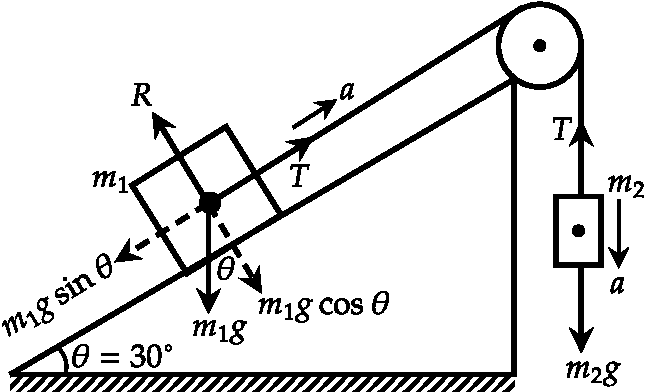
\includegraphics[height=3.5cm,width=6cm]{diagram-20220216-crop}
			\end{figure}
		\begin{align}
\text{We have }T-m_{1} g \sin \theta&=m_{1} a \label{1} \\
\text{ and }m_{2} g-T&=m_{2} a \label{2}\\
\intertext{Solving equations (\ref{1}) and (\ref{2}), we get}
a&=\frac{\left(m_{2}-m_{1} \sin \theta\right) g}{\left(m_{1}+m_{2}\right)}\label{3}\\
\text { and } \quad T & =m_{2} g\left[1-\frac{\left(m_{2}-m_{1} \sin \theta\right)}{\left(m_{1}+m_{2}\right)}\right] \notag\\
 \text { or } \quad T & =\frac{m_{1} m_{2}(1+\sin \theta) g}{\left(m_{1}+m_{2}\right)}\\
 \text{Here }m_{1}&=4 \mathrm{~kg}, m_{2}=5 \mathrm{~kg}, \theta=30^{\circ} \text{and }g=10 \mathrm{~m} / \mathrm{s}\notag\\
  \intertext{Substituting these values in equation (\ref{3}), we get}
 T&=\frac{5 \times 4\left(1+\frac{1}{2}\right) 10}{9}=\frac{300}{9}=33.33 \mathrm{~N}\notag
\end{align}
	\end{answer}
	\item A particle of mass $m$ is connected to two springs of unstretched length ' $l$ ' and spring constant $k$ as show in figure. Calculate acceleration of particle if it is slightly displaced along X-direction.
	\begin{answer}
			Let the particle is displaced by a distance $x$ along $+x$ direction as shown in figure.
			\begin{figure}[H]
				\centering
				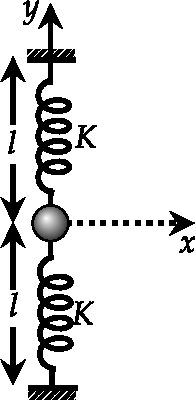
\includegraphics[height=4.5cm,width=2cm]{diagram-20220216(1)-crop}
			\end{figure}
		\begin{figure}[H]
			\centering
			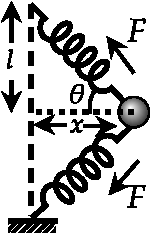
\includegraphics[height=3cm,width=2cm]{diagram-20220216(2)-crop}
		\end{figure}
		\begin{align*}
	\text{	Therefore, stretched length of spring }&=\sqrt{l^{2}+x^{2}}\\
		\text{elongation in springs }&=\sqrt{l^{2}+x^{2}}-l\\
	\text{	Restoring force on the particle due to each spring} F&=k\left(\sqrt{l^{2}+x^{2}}-l\right)
	\intertext{ Because of restoring force the particle moves back towards its initial position.}
\text{	Equation of motion of particle }F_{x}&=m \frac{d^{2} x}{d t^{2}}\\
	\text{or }-2 F \cos \theta&=m \frac{d^{2} x}{d t^{2}}\text{ or }-2 k\left(\sqrt{l^{2}+x^{2}}-l\right) \cdot \frac{x}{\sqrt{l^{2}+x^{2}}}=m \frac{d^{2} x}{d t^{2}}\\
	\text{Therefore, }\frac{d^{2} x}{d t^{2}}&=-\frac{2 k x}{m}\left(1-\frac{l}{\sqrt{l^{2}+x^{2}}}\right)\text{ or }\frac{d^{2} x}{d t^{2}}\\&=-\frac{2 k x}{m}\left[1-\left(1+\frac{x^{2}}{l^{2}}\right)^{-1 / 2}\right]\\
\text{	Since, }&x<l,\left(1+\frac{x^{2}}{l^{2}}\right)^{-1 / 2} \approx 1-\frac{x^{2}}{2 l^{2}}\\
\text{	Therefore, }\frac{d^{2} x}{d t^{2}}&=-\frac{2 k x}{m}\left[1-\left(1-\frac{x^{2}}{2 l^{2}}\right)\right]\text{ or }\frac{d^{2} x}{d t^{2}}=-\frac{k x^{3}}{m l^{2}}
		\end{align*}
	\end{answer}
\item At the moment $t=0$, the force $F=k t$ is applied to a small body of mass $m$ resting on smooth horizontal plane $(k=$ constant). The permanent direction of this force forms an angle $\theta$ with the horizontal (figure below). Find\\
\begin{figure}[H]
	\centering
	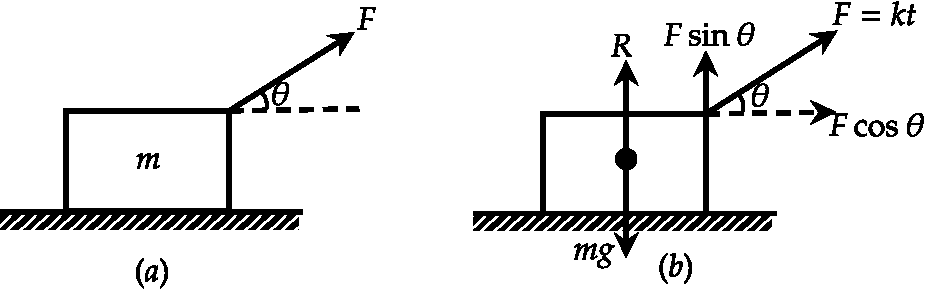
\includegraphics[height=3cm,width=10cm]{diagram-20220217-crop}
\end{figure}
(a) the velocity of the body at the moment of its breaking off the plane;\\
(b) the distance traversed by the body up to this moment.

\begin{answer}
		The free body diagram is shown in figure.
	\begin{align*}
	\text{From figure: }R+F \sin \theta&=m g\\
	\text{At breaking off, }R&=0, \therefore F=\frac{m g}{\sin \theta}\\
\text{	Now }k t&=\frac{m g}{\sin \theta}\text{ or }t=\frac{m g}{k \sin \theta}
\intertext{	(a) If $a$ be the acceleration, then $F \cos \theta=m a$ }
\text{	Therefore, }k t \cos \theta&=m \times\left(\frac{d v}{d t}\right) \quad\left(\because a=\frac{d v}{d t}\right) .
\intertext{Integrating this expression within proper limits, we get $m \int_{0}^{v} d v=k \cos \theta \int_{0}^{m g / k \sin \theta} t d t$}
\text{ or }\quad m v&=\frac{k \cos \theta}{2}\left[\frac{m g}{k \sin \theta}\right]^{2}\text{ or }v=\frac{m g^{2}}{2 k}\left(\frac{\cos \theta}{\sin ^{2} \theta}\right)\\
\text{(b) Without putting the limits, we have }v&=\frac{k \cos \theta}{2 m} t^{2}+C,\text{ where $C=$ constant of integration.}\\
\text{When }t&=0, v=0\text{ and hence }C=0.\\
\text{Now, }\frac{d s}{d t}&=\frac{k \cos \theta}{2 m} t^{2} \int_{0}^{s} d s=\frac{k \cos \theta}{2 m} \int_{0}^{m g / k \sin \theta} t^{2} d t\\
s&=\frac{k \cos \theta}{2 m}\left[\frac{t^{3}}{3}\right]_{0}^{m g / k \sin \theta} \quad\text{ or }s=\frac{m^{2} g^{3} \cos \theta}{6 k^{2} \sin ^{3} \theta} .
	\end{align*}
\end{answer}
\item Spherical particles of a given material of density $\rho$ are released from rest inside a liquid medium of lower density. The viscous drag force may be approximated by the Stoke's law, i.e, $F_{d}=6 \pi \eta R \mathrm{v}$, where $\eta$ is the viscosity of the medium, $R$ the radius of a particle and $v$ its instantaneous velocity. If $\tau(m)$ is the time taken by a particle of mass $m$ to reach half its terminal velocity, then the ratio $\tau(8 m) / \tau(m)$ is
\begin{answer}
	 Each particle has same density but different radii and masses. We have to calculate time of fall in terms of mass of particle therefore we will write our equations explicitly in terms of mass and we will remove radius from our equations wherever it appears.\\Drag force on particles
	 \begin{align}
	 F_{d}&=6 \pi \eta R \mathrm{v}, \quad\text{ Mass of a particle }m=\rho \cdot \frac{4}{3} \pi R^{3}\notag\\
	 \therefore R&=\left(\frac{3 m}{4 \pi \rho}\right)^{1 / 3} \quad \therefore F_{d}\notag\\&=6 \pi \eta\left(\frac{3 m}{4 \pi \rho}\right)^{1 / 3} v=K m^{1 / 3} v\text{, where }K=6 \pi \eta\left(\frac{3}{4 \pi \rho}\right)^{1 / 3}\notag\\
	\intertext{ If $\mathrm{B}$ is buoyancy force, then equation of motion of a particle is}\notag\\
	 m \frac{d v}{d t}&=m g-F_{d}-B\text{ where }\mathrm{B}=\frac{4}{3} \pi R^{3} \sigma g\notag\\&=\frac{4}{3} \pi R^{3} \rho g \cdot \frac{\sigma}{\rho}=m g \frac{\sigma}{\rho}, \sigma=\text{ density of medium}\notag\\
	 \therefore m \frac{d v}{d t}&=m g-K m^{1 / 3} v-m g \frac{\sigma}{\rho}, m \frac{d v}{d t}=m g\left(1-\frac{\sigma}{\rho}\right)-K m^{1 / 3} v \notag\\
	 \text { or } \frac{d v}{d t}&=g\left(1-\frac{\sigma}{\rho}\right)-K m^{-2 / 3} v\label{5}\\
	 \text{when terminal }&\text{velocity is reached }\frac{d v}{d t}=0\notag\\
	 \therefore 0&=g\left(1-\frac{\sigma}{\rho}\right)-K m^{-2 / 3} v_{t} \quad \therefore v_{t}=\frac{g\left(1-\frac{\sigma}{\rho}\right)}{K m^{-2 / 3}}\label{6}\\
	\intertext{ Now, if $\tau$ be the time to reach half the terminal velocity then from (\ref{5})}\notag\\
	 \int_{0}^{1 / 2} \frac{d v}{g\left(1-\frac{\sigma}{\rho}\right)-K m^{-2 / 3} v}&=\int_{0}^{\tau} d t, \quad \therefore-\frac{1}{K m^{-2 / 3}} \ln \left[\frac{g\left(1-\frac{\sigma}{\rho}\right)-\frac{K m^{-2 / 3} v_{t}}{2}}{g\left(1-\frac{\sigma}{\rho}\right)}\right]=\tau\notag\\
	 \text{using value of $v_{t}$ from (\ref{6}) we get, }\tau&=\frac{m^{2 / 3}}{K} \ln 2 \quad\text{ or }\quad \tau(m)=\frac{m^{2 / 3} \ln 2}{K}\notag\\
	  \therefore \tau(8 m) / \tau(m)&=(8 m)^{2 / 3} / m^{2 / 3}=4\notag
	 \end{align}
\end{answer}
\item A particle of unit mass is thrown vertically upward with initial speed $v_{0}$. It is acted upon by a drag force $b v^{2}$ in addition to gravity where $b$ is constant and $v$ is instantaneous velocity of particle. Calculate speed of the particle when it returns to the point from where it was thrown.
\begin{answer}
	In presence of drag force only quantity that is common in upward and downward motion is the distance covered.
	\begin{figure}[H]
		\centering
		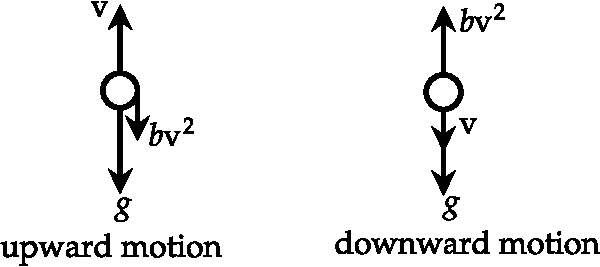
\includegraphics[height=3cm,width=7cm]{c prb01}
	\end{figure}
	\begin{align*}
	\text{For upward motion, initial speed }&=v_{0},\\
	 \text{final speed }&=0,\text{ let height reached $=h$}\\
	 \text{ equation of motion }\frac{d v}{d t}&=-g-b v^{2}\\
	\text{or }\frac{d v}{d y} \cdot \frac{d y}{d t}&=-g-b v^{3}, \frac{d y}{d t}=v\text{ or }\frac{v d v}{g+b v^{2}}=-d y\\
	\therefore \int_{v}^{0} \frac{v d v}{g+b v^{2}}&=-\int_{0}^{h} d y\\
\text{	on integration we get, }\frac{1}{2 b} \ln \left(\frac{g+b v_{0}^{2}}{g}\right)&=h\\
\text{for downward motion, initial speed }&=0,\text{ final speed $=v($ let $)$, height descended $=h$ }\\
\text{equation of motion }\frac{d v}{d t}&=g-b v^{2}\text{ or }\frac{v d v}{g-b v^{2}}=d y\text{ or }\int_{0}^{v} \frac{v d v}{g-b v^{2}}=\int_{0}^{h} d y\\
\text{on integration we get, }\frac{1}{2 b} \ln \left(\frac{g}{g-b v^{2}}\right)&=h\\
\text{Comparing (a) and (b) we get, }\frac{g+b v_{0}^{2}}{g}&=\frac{g}{g-b v^{2}}, \quad g-b v^{2}=\frac{g^{2}}{g+b v_{0}^{2}}\\
\text{or }v&=\frac{v_{0}}{\sqrt{1+\frac{b v_{0}^{2}}{g}}} \Rightarrow v<v_{0}
	\end{align*}
	due to drag force the particle returns with a speed less than its initial speed. If drag force were absent $b=0$, then $v=v_{0} .$ Therefore in absence of drag force particle returns with same speed as its initial value.
\end{answer}
\item A small ring of mass $m$ can slide on a smooth circular wire of radius $r$ and center $O$, which is fixed in a vertical plane. From a point on the wire at a vertical distance $r / 2$ above $O$, the ring is given a velocity $\sqrt{(g r) }\text { along the downward tangent to the wire. Show that it will just reach the highest point of the wire. }$ Find the reaction between the ring and the wire when the ring is at a vertical distance $r / 2$ below.
\begin{answer}
	\begin{align}
\text{At point $C$, the velocity of the ring }&=\sqrt{(r g)}.\notag\\
\text{K.E. at }C&=\frac{1}{2} m v^{2}=\frac{1}{2} m r g\text{ and P.E. at }C\notag\\&=m g h=m g(A F)=m g(r+r / 2)=\frac{3 m g r}{2}.\notag\\
\text{Total energy }&=m g r\left[\frac{1}{2}+\frac{3}{2}\right]=2 m g r.\label{7}
	\end{align}
	If the ring has to reach at $D$, with kinetic energy zero, its potential energy $=m g(2 r)$.
	Becuase the particle at $C$ has this amount of energy and it will just reach at $D$ with zero velocity.\\
	\begin{figure}[H]
		\centering
		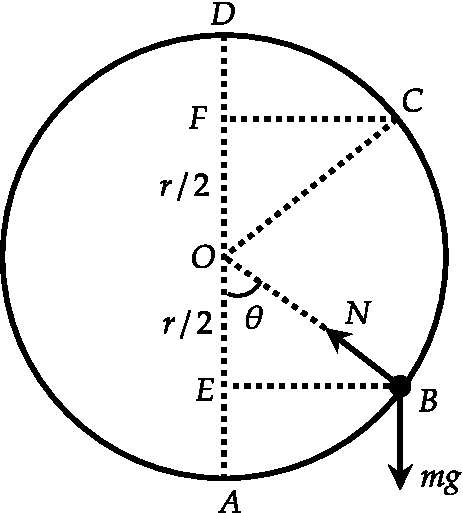
\includegraphics[height=4.8cm,width=4.5cm]{diagram-20220217(1)-crop}
	\end{figure}
	Now consider the ring at $B$, a distance $r / 2$ below $O$. Resolving $m g$ in two parts and considering the equilibrium, we get
	\begin{align}
	N-m g \cos \theta&=\frac{m v_{1}^{2}}{r}\notag\\
	N&=\frac{m v_{1}^{2}}{r}+m g \cos \theta\label{8}
	\intertext{Falling from $C$, i.e., through a distance $r$, the ring has lost a potential energy $m g r .$ This is the gain in kinetic energy.}
\text{	Hence, }\frac{1}{2} m v_{1}^{2}&=\frac{1}{2} m g r+m g r=\frac{3}{2} m g r \text{or }v_{1}^{2}=3 g r\text{ or }\frac{v_{1}^{2}}{r}=3 g.\notag\\
\text{ Fromequation (\ref{8}),} N&=m\left(3 g+g \times \frac{1}{2}\right)
	\left(\because \cos \theta=\frac{1}{2}\right)\notag\\\text{ or}& N=\left(\frac{7}{2}\right) \mathrm{mg}=3.5 \mathrm{mg}.\notag
	\end{align}
\end{answer}
\item A $2.0 \mathrm{~kg}$ block of mass, initially at rest, is dropped from a height of $0.40$ meter onto a spring whose force constant is $1960 \mathrm{nt} /$ meter. Find the maximum distance that the spring will be compressed.
\begin{answer}
	The situation is shown in figure. Let $m$ be the mass of the block and $k$ be the force constant of the spring.Let $l$ be the distance through which the spring is compressed. The total vertical fall of the block is $(h+l)$. Loss of the gravitational potential energy of the block $=m g(h+l)$.\\
	\begin{figure}[H]
		\centering
		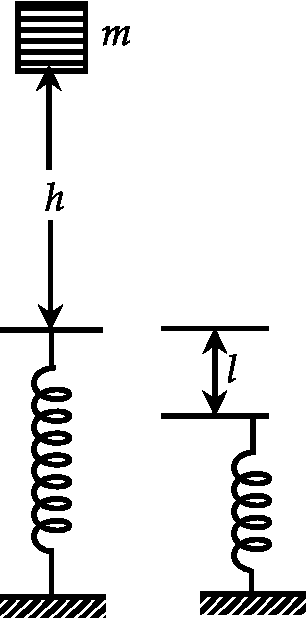
\includegraphics[height=5cm,width=2.5cm]{diagram-20220217(2)-crop}
	\end{figure}
	\begin{align*}
	\text{Elastic potential energy }&\text{in the spring }=\left(\frac{1}{2}\right) k t^{2}.
\intertext{	By the law of conservation of energy}
	m g(h+l)&=\frac{1}{2} k t^{2} \text { or } \frac{2 m g h}{k}+\frac{2 m g}{k} l=l^{2} \text { or } l^{2}-\frac{2 m g}{k} l-\frac{2 m g h}{k}=0\\
	\therefore \quad l&=\frac{\left(\frac{2 m g}{k}\right) \pm \sqrt{\left[\left(\frac{2 m g}{k}\right)^{2}+\left(\frac{8 m g h}{k}\right)\right]}}{2}\\
	\text{According to given problem, }m&=2 \mathrm{~kg}, h=0.40 \mathrm{~m} \text{and $k=1960$ newton/meter. Hence,}\\
	l&=\frac{(2 \times 2 \times 9.8 / 1960) \pm \sqrt{(2 \times 2 \times 9.8 / 1960)^{2}+(8 \times 2 \times 9.8 \times 0.40 / 1960)}}{2} \\
	l&=\mathbf{0 . 1} \text { meter. }
	\end{align*}
\end{answer}
\item A particle of mass $3 \mathrm{~kg}$ is moving under the action of a central force whose potential energy is given by $U(r)=10 r^{3}$ joule. For what energy and angular momentum will the orbit be a circle of radius $10 \mathrm{~m}$ ? Calculate the time period of this motion.
\begin{answer}
	\begin{align*}
	\text{Given that }U(r)&=10 r^{3}.
	\intertext{So the force $F$ acting on the particle is given by}
	F&=\frac{\partial U}{\partial r}=-\frac{\partial}{\partial r}\left(10 r^{3}\right)=-10 \times 3 r^{2}=-30 r^{2}\\
	\text{For circular motion of the particle }F&=\frac{m v^{2}}{r}=30 r^{2}.\\
	\text{Substituting the given values, we have }\frac{3 \times v^{2}}{10}&=30 \times(10)^{2}\text{ or }v=100 \mathrm{~m} / \mathrm{s}.\\
	\text{The total energy in circular motion}
	E&=\text{ K.E. }+\text{ P.E. }=\frac{1}{2} m v^{2}+U(r)\\&=\frac{1}{2} \times 3 \times(100)^{2}+10 \times(10)^{3}=2.5 \times 10^{4}\text{ joule}\\
	\text{Angular momentum }&=m v r=3 \times 100 \times 10=3000 \mathrm{~kg}-\mathrm{m}^{2} / \mathrm{sec}\\
	\text{Time period }T&=\frac{2 \pi r}{v}=\frac{2 \times \pi \times 10}{100}=\frac{\pi}{5} \mathrm{sec} .
	\end{align*}
\end{answer}
\item In figure, $A B C D E$ is a channel in the vertical plane, part $B C D E$ being circular with radius $r$. A ball is released from $A$ and slides without friction and without rolling. Show that it will complete the loop path if $h$ is greater than $5 r / 2$.
\begin{figure}[H]
	\centering
	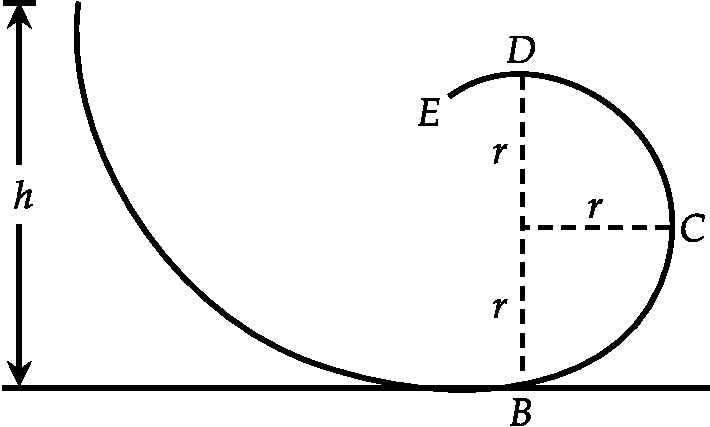
\includegraphics[height=3cm,width=5cm]{diagram-20220217(3)-crop}
\end{figure}
\begin{answer}
	\begin{align}
\intertext{	Let $m$ be the mass of the ball. When the ball comes down to $B$, its loses its potential energy $m g h$ which is converted into kinetic energy. Let $v_{B}$, be the velocity of the ball at $B$. Then,}\notag\\
	m g h&=\frac{1}{2} m v_{B}^{2}
\intertext{	The ball now rises to a point $D$, where its potential energy is $m g(h-2 r) .$ If $v_{D}$ be the velocity of the ball at $D$, then}\notag\\
	m g(h-2 r)&=\frac{1}{2} m v_{D}^{2}\label{09}
\intertext{	Now to complete the circular path, it is necessary that the centripetal force acting upward at point $D$ should be equal or greater than the force $m g$ acting downward. Therefore,}\notag\\
	\frac{m v_{D}^{2}}{r} \geq m g&\text{ or }v_{D}^{2} \geq r g\\
\text{	Fromequation (\ref{09}) }v_{D}^{2}&=2 g(h-2 r)\notag\\
	\therefore \quad 2 g(h-2 r) \geq &r g, h \geq \frac{5}{2} r .\notag
	\end{align}
\end{answer}
\item A moving particle of mass $m$ collides head-on with a particle of mass $2 m$ which is initially at rest. Show that the particle $m$ will loose $8 / 9$ th part of its initial kinetic energy after the collision.
\begin{answer}
	Let $u_{1}$ be the initial velocity of mass $m$ before collision and $v_{1}$ and $v_{2}$ the velocities of masses $m$ and $2 m$ after collision respectively.\\
	According to the law of conservation of kinetic energy, we have
	\begin{align}
 \frac{1}{2} m u_{1}^{2}&=\frac{1}{2} m v_{1}^{2}+\frac{1}{2}(2 m) v_{2}^{2}\notag \\ \text { or } & u_{1}^{2}-v_{1}^{2}=2 v_{2}^{2} \notag\\ \text { or } & \left(u_{1}-v_{1}\right)\left(u_{1}+v_{1}\right)=2 v_{2}^{2}\label{10}
\intertext{ By the law of conservation of momentum, we have}\notag
 m u_{1}&=m v_{1}+(2 m) v_{2} \notag\\
 \left(u_{1}-v_{1}\right)&=2 v_{2}\label{11}\\
\text{ From eqs. (\ref{10}) and (\ref{11}), we get }\left(u_{1}+v_{1}\right)&=v_{2}\label{12}
\intertext{ Substituting the value of $v_{2}$ from eq. (\ref{12}) in eq. (\ref{11}), we get}\notag\\
u_{1}-v_{1}=2\left(u_{1}+v_{1}\right) \text { or }-3 v_{1}&=u_{1} \text { or } v_{1}=-\left(\frac{1}{3}\right) u_{1}\label{13}
\intertext{Now the initial and final kinetic energies of mass $m$ are}
K_{i}=\left(\frac{1}{2}\right) m u_{1}^{2} \text { and } K_{f}&=\left(\frac{1}{2}\right) m v_{1}^{2}=\left(\frac{1}{2}\right) m\left(\frac{u_{1}^{2}}{9}\right)\notag\\
\text{Therefore, fraction loss }&=\frac{K_{i}-K_{f}}{K_{i}}=\frac{\frac{1}{2} m u_{1}^{2}\left(1-\frac{1}{9}\right)}{\frac{1}{2} m u_{1}^{2}}=\frac{8}{9}\notag
	\end{align}
\end{answer}
\item A solid hemisphere of mass $M$ and radius $R$ is placed against a smooth wall as shown in the figure. what is normal reaction on the sphere due to the wall.
\begin{answer}
	Centre of mass of the hemisphere lies at a distance $\frac{3 R}{8}$ from
	its base centre. The sphere is in equilibrium therefore torque about point A must be zero.
	\begin{figure}[H]
		\centering
		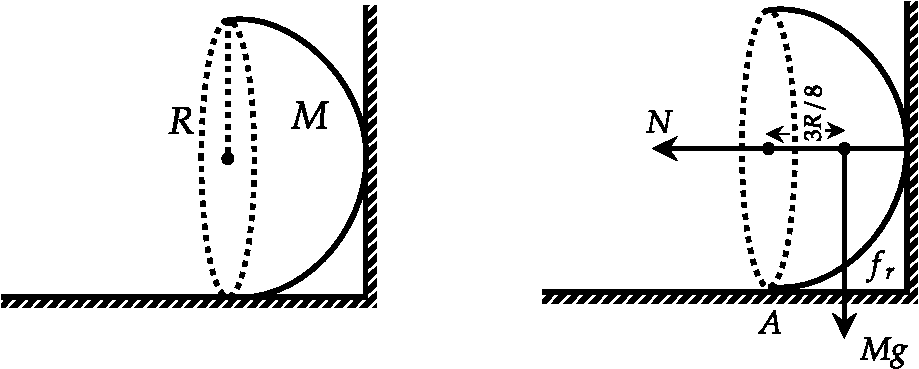
\includegraphics[height=3.2cm,width=9cm]{diagram-20220217(4)-crop}
	\end{figure}
	\begin{align*}
	\therefore N R-M g \cdot \frac{3 R}{8}&=0\\
	\text{or, }N&=\frac{3 M g}{8}
	\end{align*}
\end{answer}
\item A thin rod of mass $M$ and length $L$ is suspended from one end while its other end lies on a smooth horizontal plane and makes an angle $\alpha$ with the plane. Find the normal reaction from the plane and tension in the string from which it is suspended.
\begin{figure}[H]
	\centering
	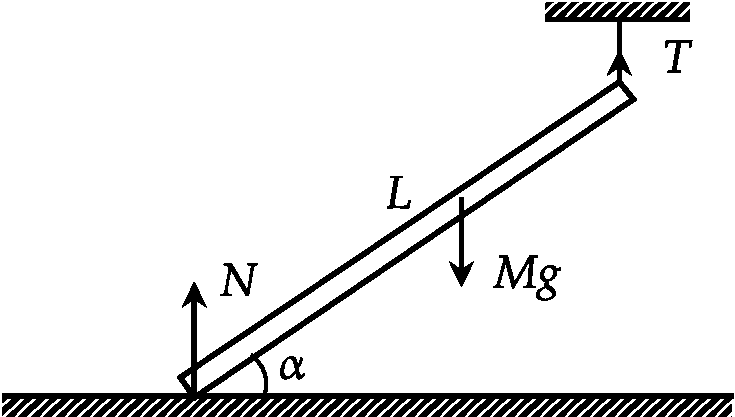
\includegraphics[height=3cm,width=5cm]{diagram-20220217(5)-crop}
\end{figure}
\begin{align}
\text{For translational equilibrium }T+N&=M g \label{14}\\
\text{For rotational }&\text{equilibrium }\notag\\
\text{Torque about lower}&\text{ end of the rod is zero}\notag\\
	\therefore T . L \cos \alpha-M g \frac{L}{2} \cos \alpha&=0 \quad \therefore \quad T=\frac{M g}{2}\notag\\
	\text{from (\ref{14}) }N&=M g-T=M g-\frac{M g}{2}=\frac{M g}{2}\notag
\end{align}
Example: A uniform ladder of length 2L and mass 'm' leans against a wall in a vertical plane at an angle $\theta$ to the horizontal. The floor is rough, having a coefficient of static friction $\mu$
A person of mass $M$ stands on the ladder at a distance $D$ from its base (see figure). If the wall is frictionless, the maximum distance $\left(D_{\max }\right)$ up the ladder that the person can reach before the ladder slips is
\begin{figure}[H]
	\centering
	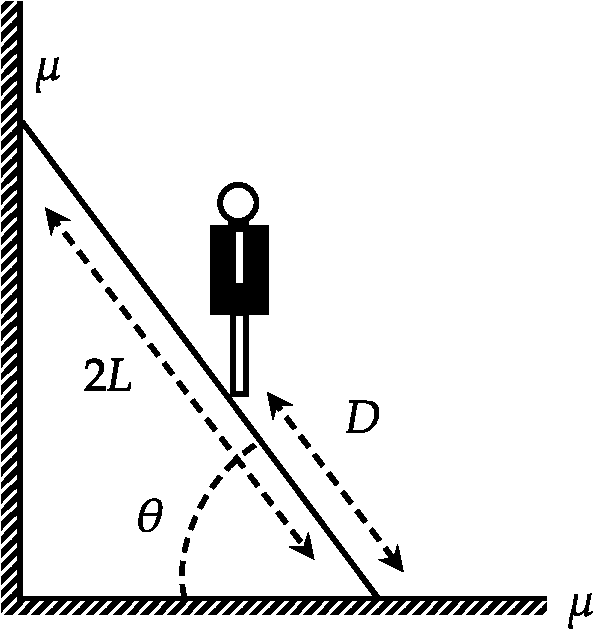
\includegraphics[height=4cm,width=4cm]{diagram-20220217(6)-crop}
\end{figure}
\begin{answer}
	Let us take ladder plus person as system. Various forces acting on the system are shown in the figure. For translational equilibrium we must have
	\begin{align}
	N_{1}&=(M+m) g\label{15}\\
	N_{2}&=f_{r}\label{16}\\
	\intertext{	For rotational equilibrium torque about lower end of the ladder must be zero. Therefore,}\notag\\
	M g D \cos \theta+m g L \cos \theta-N_{2} .2 L \sin \theta&=0\notag\\
	\therefore N_{2}&=\frac{g \cot \theta}{2}\left[\frac{M D}{L}+m\right]\notag\\
	\therefore\text{ from (\ref{16}) we get, }f_{r}&=\frac{g \cot \theta}{2}\left[\frac{D}{L} M+m\right]\notag\\
	\text{since }f_{r} \leq \mu N_{1}, \quad &\therefore \frac{g \cot \theta}{2}\left[\frac{D}{L} M+m\right] \leq \mu(M+m) g\notag\\
\text{	or }D \leq \frac{L}{M}[2 \mu(M+m) \tan \theta-m] \quad &\therefore D_{\max }=L\left[2 \mu\left(1+\frac{m}{M}\right) \tan \theta-\frac{m}{M}\right]\notag
	\end{align}
 \begin{figure}[H]
 	\centering
 	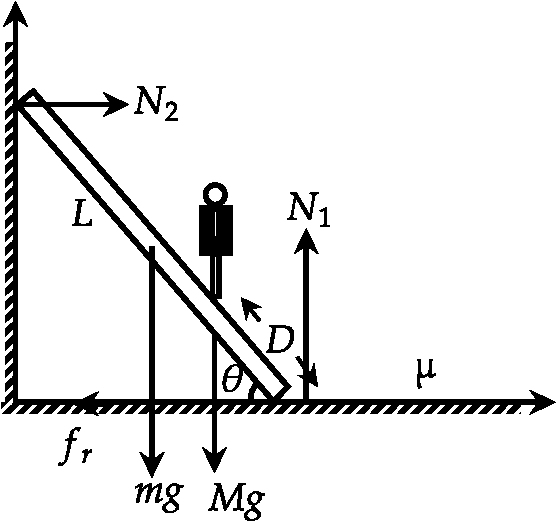
\includegraphics[height=4.5cm,width=4.5cm]{diagram-20220217(7)-crop}
 \end{figure}
\end{answer}
\item A body of mass $m$ rests on a horizontal plane with the friction coefficient $\mu .$ At the moment $t=0$, a horizontal force is applied to it, which varies with time $F=k t$, where $k$ is a constant vector. Find the distance traversed by the body during first/seconds after the force action began.
\begin{answer}
	Here just after applying the force, the motion does not start due to friction force. As the applied force is proportional to time, let after a time $t_{0}$, the motion starts.
	\begin{align*}
	\text{Now, }F=k t_{0}=\mu m g\text{ or }t_{0}=\left(\frac{\mu m g}{k}\right)
\intertext{	If $t \leq t_{0}$, the distance traversed by the body $s=0 .$}
\text{	When }t \leq t_{0},\text{ then }F&=k\left(t-t_{0}\right)
	\end{align*}
		\begin{align}
	\therefore \quad m \frac{d v}{d t}&=k\left(t-t_{0}\right)\text{ or }m d v=k\left(t-t_{0}\right) d t \ldots \label{17}\\
\text{	Integrating equation (\ref{17}), we get } m v&=\frac{k}{2}\left(t-t_{0}\right)^{2}+C_{1}\notag\\
	\text{When }t&=t_{0}, v=0, \therefore C_{1}=0\notag\\
	\therefore \quad m v&=\frac{k}{2}\left(t-t_{0}\right)^{2}\\
	\text{Again }m \frac{d s}{d t}&=\frac{k}{2}\left(t-t_{0}\right)^{2}\text{ or }m d s=\frac{k}{2}\left(t-t_{0}\right)^{2} d t\label{19}\\
	\text{Integrating equation (\ref{19}), we get }s&=\frac{k}{6 m}\left(t-t_{0}\right)^{3}+C_{2}\notag\\
\text{	Here }C_{2}&=0\text{ because when }t=t_{0}, s=0\notag\\
	\therefore \quad s&=\frac{k}{6 m}\left(t-t_{0}\right)^{3} .\notag
	\end{align}
\end{answer}
\item A falling rain drop accumulates moisture due to which its radius increases at a constant rate $k$. Neglecting drag calculate the speed of rain drop after it has fallen for a time $t$.
\begin{answer}
	\begin{align}
	\text{Equation of motion }\frac{d p}{d t}&=m g\label{20}\\
	\text{given }\frac{d r}{d t}&=k \Rightarrow r=k t\text{ (if initial radius is zero)}\notag\\
	\text{since }m&=\frac{4}{3} \pi r^{3} \rho \quad \therefore \frac{d m}{d t}=4 \pi r^{2} \cdot \frac{d r}{d t} \cdot \rho\notag
\intertext{	$\rho$ is density, we assume it to be constant}\notag
	\frac{d m}{d t} &=\left(\frac{4}{3} \pi r^{3} \rho\right) \cdot \frac{3 k}{r} \notag\\
	\frac{d m}{d t} &=\frac{3 m k}{r}\label{21}\\
\intertext{	Dividing (\ref{20}) by (\ref{21}) we get}\notag
\frac{d p}{d m}&=\frac{g}{3 k} r \quad d p=\left(\frac{g}{3 k}\right) \cdot\left(\frac{3 m}{4 \pi \rho}\right)^{1 / 3} d m\notag\\
\intertext{on integration we get}\notag
\therefore \quad p&=\left(\frac{g}{3 k}\right)\left(\frac{3}{4 \pi \rho}\right)^{1 / 3} \cdot \frac{m^{4 / 3}}{4 / 3}+c\notag\\
\text{taking }p&=m=0\text{ at }t=0,\text{ we get }c=0\notag\\
\therefore \quad p&=\frac{g}{4 k}\left(\frac{3}{4 \pi \rho}\right)^{1 / 3} \cdot m^{4 / 3}\notag\\
\text{or }v&=\left(\frac{g}{4 k}\right) \cdot\left(\frac{3 m}{4 \pi \rho}\right)^{1 / 3}\notag\\
v&=\frac{g}{4 k} r \Rightarrow v=\frac{g}{4} t\notag
	\end{align}
\end{answer}
	\item A particle of mass $2 \mathrm{~kg}$ is moving such that at time $t$, its position, in metre, is given by $\vec{r}(t)=5 \hat{i}-2 t^{2} \hat{j}$. The angular momentum of the particle at $t=2 \mathrm{~s}$ about the origin, in $\mathrm{kg} \mathrm{m}^{2} \mathrm{~s}^{-1}$, is
	 \begin{tasks}(4)
		\task[\textbf{a.}]$-40 \hat{k}$
		\task[\textbf{b.}]$-80 \hat{k}$
		\task[\textbf{c.}]$80 \hat{k}$
		\task[\textbf{d.}]  $40 \hat{k}$
	\end{tasks}
	\begin{answer}
		\begin{align*}
		\vec{r} &=5 \hat{i}-2 t^{2} \hat{j} \\
		\vec{v} &=\frac{d \vec{r}}{d t}=-4 t \hat{j} \\
		\vec{p} &=m \vec{v}=2(-4 t \hat{j})=-8 t \hat{j} \\
		\vec{L} &=\vec{r} \times \vec{p}=\left(5 \hat{i}-2 t^{2} \hat{j}\right) \times(-8 t \hat{j}) \\
		&=-40 t \hat{k}=-40 \times 2 \hat{k}=-80 \hat{k}
		\end{align*}
			Hence correct answer is (b)
	\end{answer}
	\item The scalar potential corresponding to the force field $\vec{F}=\hat{i}(y+z)$
	 \begin{tasks}(4)
		\task[\textbf{a.}]Is $y^{2} / 2$
		\task[\textbf{b.}] Is 1
		\task[\textbf{c.}]Is zero
		\task[\textbf{d.}] Does not exist
	\end{tasks}
	\begin{answer}
		\begin{align*}
		\vec{F} &=\hat{i}(y+z) \\
	\vec{\nabla} \times \vec{F}&=\left|\begin{array}{ccc}\hat{i} & \hat{j} & \hat{k} \\ \frac{\partial}{\partial x} & \frac{\partial}{\partial y} & \frac{\partial}{\partial z} \\ y+z & 0 & 0\end{array}\right|=\hat{i}(0-0)-\hat{j}(0-1)+\hat{k}(0-1)=-\hat{j}-\hat{k} \neq 0
		\end{align*}
			Force is not conservative so we cannot define potential. \\Hence, correct answer is (d)
	\end{answer}
\end{enumerate}
\section{Stability Analysis}
\begin{enumerate}
	\item  A particle of mass $m$ is moving under a one dimensional potential $V(x)=-a x+b x^{2}$ where $a>$ 0 and $b>0$. Find the equilibrium points and find frequency of oscillation about the stable equilibrium.
	\begin{answer}
		\begin{align*}
		\text{At equilibrium point, }\left.\frac{d V}{d x}\right|_{x=x_{0}}=0\\
		\therefore-a+2 b x_{0}=0 \quad\text{ or }\quad x_{0}&=\frac{a}{2 b}\\
	\text{	Thus, }x_{0}&=\frac{a}{2 b}\text{ is an equilibrium point.}
\intertext{	To know whether it is stable or To know whether it is stable or unstable equilibrium point let us calculate second derivative of potential at equilibrium point.}
	\left.\frac{d^{2} V}{d x^{2}}\right|_{x=x_{0}}&=2 b>0\\
	\text{Therefore }x_{0}=\frac{a}{2 b}&\text{ is stable equilibrium point, force constant }k=\left.\frac{d^{2} V}{d x^{2}}\right|_{x=x_{0}}=2 b
	\intertext{Therefore, frequency of oscillation is}
	\omega&=\sqrt{\frac{k}{m}}=\sqrt{\frac{2 b}{m}}
		\end{align*}
	\end{answer}
	\item  Potential corresponding to force between the atoms of a diatomic molecule is $V(r)=\frac{a}{r^{12}}-\frac{b}{r^{6}}$ where $a$ and $b$ are positive constants and $r$ is separation between the atoms. Calculate bond length for stable configuration and also calculate frequency of oscillation of atoms if mass of each atom be $m$.
	\begin{answer}
		\begin{align*}
	\text{	For stable configuration }\left.\frac{d V}{d r}\right|_{r=r_{0}}&=0\\
		-\frac{12 a}{r_{0}^{13}}+\frac{6 b}{r_{0}^{7}}=0 \Rightarrow r_{0}&=\left(\frac{2 a}{b}\right)^{1 / 6}\\
		\text{Therefore bond length for stable configuration is }&\left(\frac{2 a}{b}\right)^{1 / 6}\\
		\text{Force constant }k=\left.\frac{d^{2} V}{d r^{2}}\right|_{r=r_{0}}&=\frac{12 \times 13 a}{r_{0}^{14}}-\frac{6 \times 7 b}{r_{0}^{8}}=\frac{1}{r_{0}^{8}}\left(\frac{12 \times 13 a}{r_{0}^{6}}-6 \times 7 b\right)\\
		&=\left(\frac{b}{2 a}\right)^{8 / 6}\left(\frac{12 \times 13 a}{2 a / b}-42 b\right)\\&=\left(\frac{b}{2 a}\right)^{4 / 3} \cdot 36 b=\frac{18}{2^{1 / 3}} \cdot \frac{b^{7 / 3}}{a^{4 / 3}}\\
		\text{Reduced mass of system }\mu&=\frac{m \cdot m}{m+m}=m / 2\\
		\text{Frequency of oscillation} \omega=\sqrt{\frac{k}{\mu}}&=\sqrt{\frac{18}{2^{1 / 3}} \cdot \frac{b^{7 / 3}}{m / 2 a^{4 / 3}}}=6\left(\frac{b^{7}}{2 m^{3} a^{4}}\right)^{1 / 6}
		\end{align*}
	\end{answer}
	
	\item  A particle of mass ' $m$ ' is moving under potential $V(x)=a x^{3}-b x^{2}$. Initially the particle is at at stable point. What minimum speed be given to the particle so that it reaches unstable point. Plot potential versus $x$.
	\begin{answer}
		\begin{align*}
		\text{For equilibrium point }\left.\frac{d V}{d x}\right|_{x=x_{0}}&=0\\
		3 a x_{0}^{2}-2 b x_{0}&=0 \Rightarrow x_{0}=0, \frac{2 b}{3 a}\\
		\left.\frac{d^{2} V}{d x^{2}}\right|_{x=x_{0}}&=6 a x_{0}-2 b,\left.\frac{d^{2} V}{d x^{2}}\right|_{x=0}=-2 b<0, \therefore x_{0}=0\text{ is unstable point }\\
		\left.\frac{d^{2} V}{d x^{2}}\right|_{x=\frac{2 b}{3 a}}&=2 b>0, \therefore x_{0}=\frac{2 b}{3 a}\text{ is stable point}
		\intertext{To calculate speed let us apply conservation of energy.}
		\text{Total energy initial }&=\text{ Total energy final}
		\intertext{(Kinetic Energy + Potential Energy) at $x=\frac{2 b}{a}=($ Kinetic Energy $+$ Potential Energy) at $x=0$ for minimum speed $(u)$ at stable point the particle will just reach unstable point and stops there.}
			\therefore \frac{1}{2} m u^{2}+V\left(x=\frac{2 b}{3 a}\right)&=\frac{1}{2} m .0^{2}+V(x=0)\\
		\frac{1}{2} m u^{2}+a\left(\frac{2 b}{3 a}\right)^{3}-b\left(\frac{2 b}{3 a}\right)^{2}&=0+0\\
		u^{2}=-\frac{2}{m}\left(\frac{2 b}{3 a}\right)^{2}\left(\frac{2 b}{3}-b\right)&=\frac{2}{m} \cdot \frac{4 b^{2}}{9 a^{2}} \cdot \frac{b}{3}=\frac{8 b^{3}}{27 m a^{2}}\\
		\therefore u&=\sqrt{\frac{8 b^{3}}{27 m a^{2}}}
		\end{align*}
		\begin{figure}[H]
			\centering
			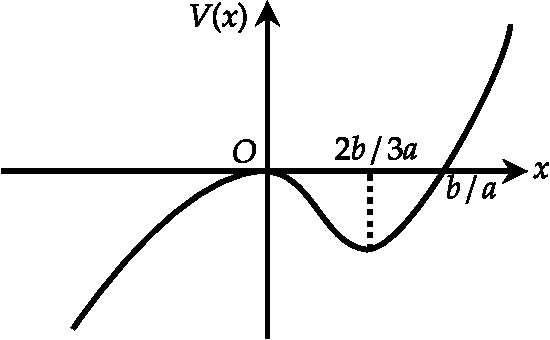
\includegraphics[height=3cm,width=5cm]{stability001}
		\end{figure}
	\end{answer}
	\item  A particle is moving under potential $V(r)=\frac{a}{r^{2}}-\frac{b}{r} .$ Calculate the minimum value of potential energy.
	\begin{answer}
		\begin{align*}
	\text{	For potential to be minimum }\left.\frac{d V}{d r}\right|_{r=r_{0}}=0\\
	 -\frac{2 a}{r_{0}^{3}}+\frac{b}{r_{0}^{2}}=0 \quad \therefore r_{0}&=\frac{2 a}{b}\\
	 \left.\frac{d^{2} V}{d r^{2}}\right|_{r=r_{0}}=\frac{6 a}{r_{0}^{4}}-\frac{2 b}{r_{0}^{3}}&=\frac{1}{r_{0}^{3}}\left(\frac{6 a}{r_{0}}-2 b\right)=\frac{1}{r_{0}^{3}}\left(\frac{6 a}{2 a / b}-2 b\right)=\frac{b}{r_{0}^{3}}>0\\
	 \text{Therefore at }r&=r_{0}\text{ potential is minimum}\\
	 \therefore \quad V_{\min }&=V\left(r_{0}\right)=\frac{1}{r_{0}}\left(\frac{a}{r_{0}}-b\right)=-\frac{b^{2}}{4 a}
		\end{align*}
	\end{answer}
	\item  A cube is placed on the top of a fixed hemisphere as shown in figure. What should be relation between length of side of cube and radius of hemisphere so that cube has stable equilibrium.
		\begin{figure}[H]
		\centering
		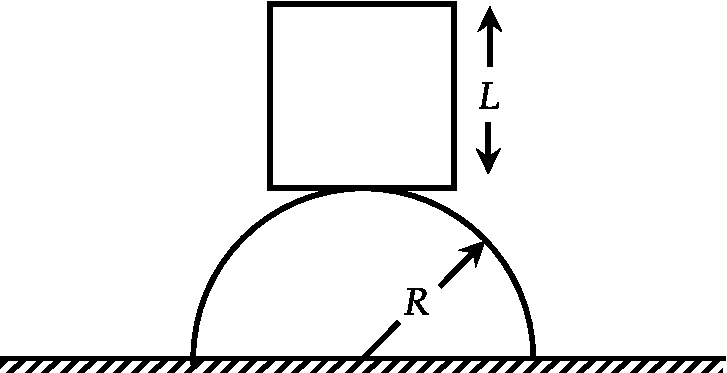
\includegraphics[height=3cm,width=6cm]{diagram-20220219(2)-crop}
	\end{figure}
	\begin{answer}
		$\left. \right. $
		\begin{figure}[H]
			\centering
			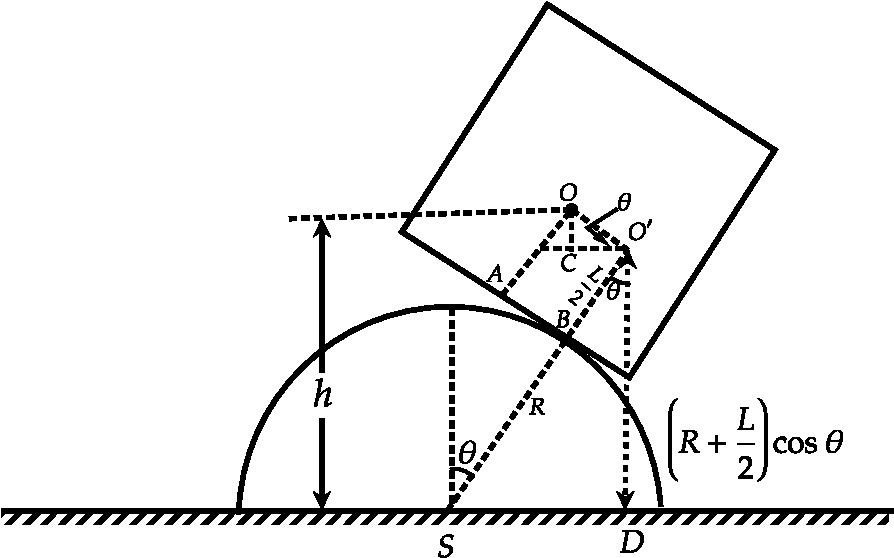
\includegraphics[height=5.5cm,width=9cm]{diagram-20220219(3)-crop}
		\end{figure}
		To discuss equilibrium of cube we first write its potential energy as function of angle from its equilibrium position. As shown in the figure below, initially point A was in contact with spherical surface but now in displaced position point $\mathrm{B}$ is in contact. Therefore,
		\begin{align*}
		A B&=R \theta
		\intertext{Height of centre of cube from centre level of hemisphere is}
		h&=O C+O^{\prime} D \\
		&=O O^{\prime} \sin \theta+O^{\prime} S \cos 0 \\
		&=A B \sin \theta+\left(O^{\prime} B+B S\right) \cos \theta \\
		&=R \theta \sin \theta+\left(\frac{L}{2}+R\right) \cos \theta
		\intertext{Potential energy of the cube}
		V(\theta)&=M g h=M g\left[R \theta \sin \theta+\left(\frac{L}{2}+R\right) \cos \theta\right]
		\intertext{$\theta=0$ is equilibrium position of the cube. For this position to be stable equilibrium position, $\left.\frac{d^{2} V}{d \theta^{2}}\right|_{\theta=0}>0$}
	&\therefore \frac{d^{2}}{d \theta^{2}} M g\left[R \theta \sin \theta+\left(\frac{L}{2}+R\right) \cos \theta\right]_{\theta=0}>0\\
&\text{	or }\frac{d}{d \theta}\left[R \theta \cos \theta+R \sin \theta-\left(\frac{L}{2}+R\right) \sin \theta\right]_{\theta=0}>0\\
	&\text{or }\left[R \cos \theta-R \theta \sin \theta+R \cos \theta-\left(\frac{L}{2}+R\right) \cos \theta\right]_{\theta=0}>0\\
	&\text{or }\left[2 R-\left(\frac{L}{2}+R\right)\right]>0 \quad \therefore R-\frac{L}{2}>0\text{ or }\quad 2 R>L
	\intertext{Thus, cube can be in stable equilibrium position if its side length is less than diameter of hemisphere}
		\end{align*}
	\end{answer}
	\item  For the mass pulley system shown in figure, what should be relation between $m$ and $M$ so that system remains in stable equilibrium position. Pulley are smooth and strings are tight and inextensible
	\begin{figure}[H]
		\centering
		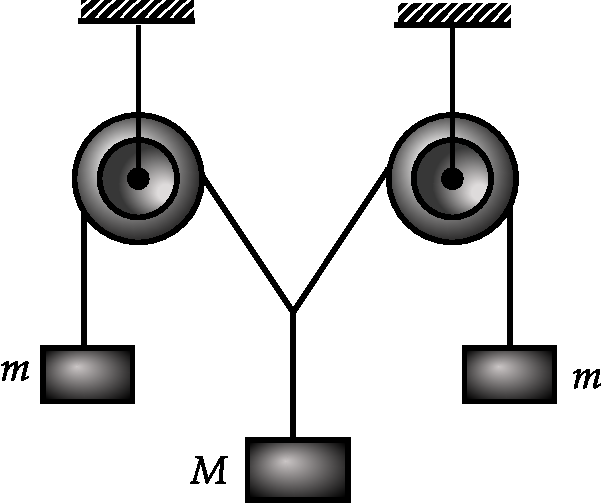
\includegraphics[height=4cm,width=5cm]{diagram-20220218(4)-crop}
	\end{figure}
	\begin{answer}
		The pulleys are fixed. Therefore we can write potential energy of the system by specifying position of blocks with respect to pulleys.\\
		Let ' $l$ ' be length of string and ' $d$ ' be the half distance between two pulleys. Therefore, $l$ and $d$ are constants If $x$ be distance of $m$ below the pulley as shown in figure then potential energy of system is
		\begin{figure}[H]
			\centering
			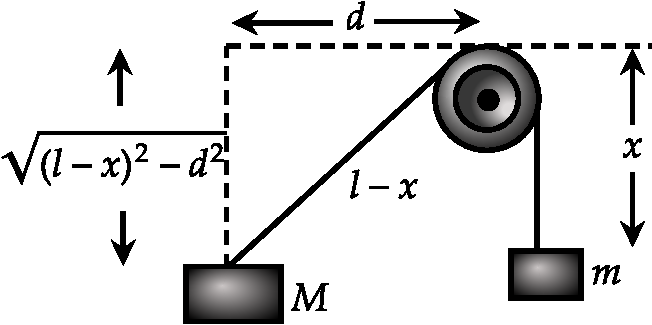
\includegraphics[height=3cm,width=6cm]{diagram-20220219(4)-crop}
		\end{figure}
		\begin{align}
		V(x)=-2 m g x-M g \sqrt{(l-x)^{2}-d^{2}} \quad &\therefore \frac{d V}{d x}=-2 m g+\frac{M g(l-x)}{\sqrt{(l-x)^{2}-d^{2}}}\notag\\
		\text{for equilibrium }\left.\frac{d V}{d x}\right|_{x=x_{0}}=0 \quad &\therefore-2 m g+\frac{M g\left(l-x_{0}\right)}{\sqrt{\left(l-x_{0}\right)^{2}-d^{2}}}=0\notag\\
	\text{	or }\frac{2 m}{M}&=\frac{l-x_{0}}{\sqrt{\left(l-x_{0}\right)^{2}-d^{2}}}\label{23}\\
	\left.\frac{d^{2} V}{d x^{2}}\right|_{x=x_{0}}&=\frac{M g d^{2}}{\left[\left(l-x_{0}\right)^{2}-d^{2}\right]^{3 / 2}}>0\text{ for all values of $d>0$}\notag\\
	\text{since, }\frac{l-x_{0}}{\sqrt{\left(l-x_{0}\right)^{2}-d^{2}}}>1 \quad &\therefore\text{ from (\ref{23}) }\frac{2 m}{M}>1\text{ or }2 m>M\notag
		\end{align}
	\end{answer}
\item The potential energy between two atoms are given $v(r)=\frac{a}{r^{12}}-\frac{b}{r^{6}}$ where $a, b$ positive constants.
(i) Find the equilibrium distance of two atoms.\\
(ii) Plot the potential\\
(iii) Calculate the frequency of small oscillation.\\
	\begin{answer}
		\begin{align*}
		\intertext{(i) For equilibrium potential energy should be minimum.}
		\frac{\mathrm{dU}}{\mathrm{dr}}=-\frac{12 \mathrm{a}}{\mathrm{r}^{13}}+\frac{6 \mathrm{~b}}{\mathrm{r}^{7}}&=0 \Rightarrow \mathrm{r}^{6}=\frac{2 \mathrm{a}}{\mathrm{b}} \\
		\mathrm{r}=\left(\frac{20}{\mathrm{~b}}\right)^{1 / 6}&=\mathrm{r}_{0} \\
		\mathrm{U}\left(\mathrm{r}_{0}\right)=\frac{\mathrm{ab}^{2}}{4 \mathrm{a}^{2}}-\frac{\mathrm{b} \cdot \mathrm{b}}{2 \mathrm{a}}&=\frac{\mathrm{b}^{2}}{4 \mathrm{a}}-\frac{\mathrm{b}^{2}}{2 \mathrm{a}}=-\frac{\mathrm{b}^{2}}{4 \mathrm{a}}\\
		\frac{\mathrm{dU}}{\mathrm{dr}}=-\frac{12 \mathrm{a}}{\mathrm{r}^{13}}+\frac{6 \mathrm{~b}}{\mathrm{r}^{7}}&=0 \Rightarrow \mathrm{r}^{6}=\frac{2 \mathrm{a}}{\mathrm{b}}\\ \mathrm{r}=\left(\frac{20}{\mathrm{~b}}\right)^{1 / 6}&=\mathrm{r}_{0} \quad[\text{ Position of stability equilibrium }]\\ \mathrm{U}\left(\mathrm{r}_{0}\right)=\frac{\mathrm{ab}^{2}}{4 \mathrm{a}^{2}}-\frac{\mathrm{b} \cdot \mathrm{b}}{2 \mathrm{a}}&=\frac{\mathrm{b}^{2}}{4 \mathrm{a}}-\frac{\mathrm{b}^{2}}{2 \mathrm{a}}=-\frac{\mathrm{b}^{2}}{4 \mathrm{a}}
			\end{align*}
			\begin{figure}[H]
				\centering
				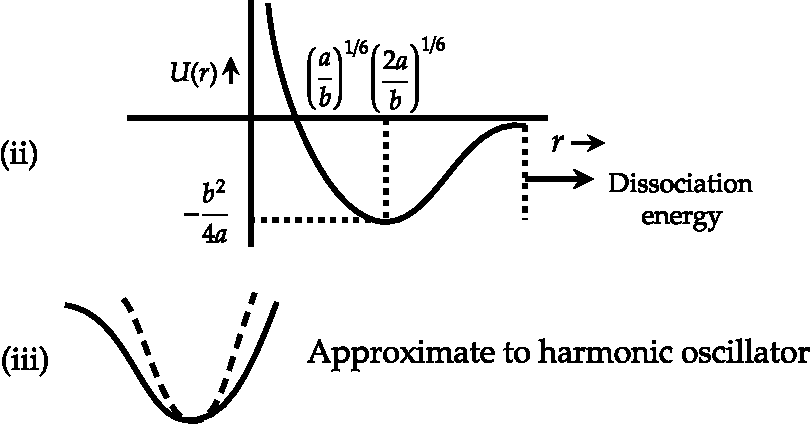
\includegraphics[height=5cm,width=9cm]{diagram-20220219(5)-crop}
			\end{figure}
				\begin{align*}
		\mathrm{U}\left(\mathrm{r}_{0}\right)=\frac{-\mathrm{b}^{2}}{4 \mathrm{a}} ; \mathrm{U}(\mathrm{r})&=\mathrm{U}\left(\mathrm{r}_{0}\right)+\left.\left(\mathrm{r}-\mathrm{r}_{0}\right) \frac{\mathrm{dU}}{\mathrm{dr}}\right|_{\mathrm{r}_{0}}+\left.\frac{\left(\mathrm{r}-\mathrm{r}_{0}\right)^{2}}{2} \frac{\mathrm{d}^{2} \mathrm{U}}{\mathrm{dr}^{2}}\right|_{\mathrm{c}_{0}}\\
		\frac{\mathrm{d}^{2} \mathrm{U}}{\mathrm{dr}^{2}}=\frac{12 \times 13 \mathrm{a}}{\mathrm{r}^{14}}-\frac{42 \mathrm{~b}}{\mathrm{r}^{8}} ;\left.\frac{\mathrm{d}^{2} \mathrm{U}}{\mathrm{dr}^{2}}\right|_{\mathrm{k}_{0}}&=\frac{156 \mathrm{a}}{\mathrm{r}^{14}}-\frac{42 \mathrm{~b}}{\mathrm{r}^{8}}=\frac{156 \mathrm{a}}{(2 \mathrm{a})^{1 / 6}}-\frac{42 \mathrm{~b}}{\left(\frac{2 \mathrm{a}}{\mathrm{h}}\right)^{3 / 6}}\\
		&=\frac{156 \mathrm{a}}{\left(\frac{2 \mathrm{a}}{\mathrm{b}}\right)^{1 / 3}}-\frac{42 \mathrm{~b}}{\left(\frac{2 \mathrm{a}}{\mathrm{b}}\right)^{1 / 3}}=\text { constant }=c\\
	\intertext{	(Force constant equivalent to spring constant)}
		U(r)&=U\left(r_{0}\right)+\frac{c}{2}\left(r-r_{0}\right)^{2}\\
		\text{So, the force }&=-\frac{\mathrm{dU}}{\mathrm{dr}}=-\frac{\mathrm{c}}{2} \cdot 2\left(\mathrm{r}-\mathrm{r}_{0}\right)^{2}=-\mathrm{c}\left(\mathrm{r}-\mathrm{r}_{0}\right)\\
		\text{Force }&=-\nabla U ; U=U(r)\text{ only}\\
		\overrightarrow{\mathrm{F}}&=\mathrm{m} \overline{\mathrm{a}} \text{(Here introduced to harmonic oscillator maynecessary).}\\
		 \text{Equation of motion, }&\mathrm{m} \frac{\mathrm{d}^{2} \mathrm{r}}{\mathrm{dt}^{2}}=-\mathrm{c}\left(\mathrm{r}-\mathrm{r}_{0}\right) ; \frac{\mathrm{d}^{2} \mathrm{r}}{\mathrm{dt}^{2}}+\frac{\mathrm{c}}{\mathrm{m}}\left(\mathrm{r}-\mathrm{r}_{0}\right)=0\\
		 \text{ Take }\mathrm{c}&=m \omega^{2} ; \omega=\sqrt{\frac{\mathrm{c}}{\mathrm{m}}}
		 \intertext{A particle of mass ' $\mathrm{m}$ ' moving in a potential} \mathrm{V}(\mathrm{x})&=\frac{1}{2} \mathrm{~m} \omega_{0}^{2} \mathrm{x}^{2}+\frac{\mathrm{a}}{2 \mathrm{~m} \mathrm{x}^{2}} \quad\left(\omega_{0} \&\right. \text{are constant })
		 \intertext{ Find the angular trequency of small oscillation.}
		\frac{\mathrm{dv}}{\mathrm{dx}}&=m \omega_{0}^{2} \mathrm{x}-\frac{\mathrm{a}}{\mathrm{m} \mathrm{x}^{3}}=0\\
		m \omega_{0}^{2} x_{0}-\frac{a}{m x^{3}}&=0 ; x_{0}^{4}=\frac{a}{m^{2} \omega_{0}^{2}} ; \chi_{0}=\left(\frac{a}{m^{2} \omega_{0}^{2}}\right)^{1 / 4}\\
		\text{Equilibrium distance, }\frac{d^{2} z}{d x^{2}}&=m \omega_{0}^{2}+\frac{3 a}{m x^{4}}\\
		\left.\frac{\mathrm{d}^{2} \mathrm{r}}{\mathrm{dx}^{2}}\right|_{\mathrm{x}=\mathrm{x}_{0}}&=m \omega_{0}^{2}+\frac{3 \mathrm{a}}{\mathrm{ma}} \mathrm{m}^{2} \omega^{2}=4 \mathrm{~m} \omega_{0}^{2} \quad\left(\mathrm{x}_{0}^{4}=\frac{\mathrm{a}}{\mathrm{m}^{2} \omega_{0}^{2}}\right)\\
		\mathrm{U}(\mathrm{x})&=\mathrm{U}\left(\mathrm{x}_{0}\right)+\left.\left(\mathrm{x}-\mathrm{x}_{0}\right) \frac{\mathrm{dU}}{\mathrm{dx}}\right|_{\mathrm{x}=\mathrm{x}_{0}}+\left.\frac{\left(\mathrm{x}-\mathrm{x}_{0}\right)^{2}}{2} \frac{\mathrm{d}^{2} \mathrm{U}}{\mathrm{dx}^{2}}\right|_{\mathrm{x}=\mathrm{x}_{0}}\\
		&=\mathrm{U}\left(\mathrm{x}_{0}\right)+\left(\mathrm{x}-\mathrm{x}_{0}\right)^{2} 2 \mathrm{~m} \omega_{0}^{2}\\
		\text{Force }&=-\frac{\mathrm{dU}}{\mathrm{dx}}=-4 \mathrm{~m} \omega_{0}^{2}\left(\mathrm{x}-\mathrm{x}_{0}\right)\\
	\text{	Equation of motion, }\mathrm{m} \frac{\mathrm{d}^{2} \mathrm{x}}{\mathrm{dt}^{2}}&=\mathrm{F}=-4 \omega_{0}^{2}\left(\mathrm{x}-\mathrm{x}_{0}\right)\\
		\frac{d^{2} x}{d t^{2}}+4 \omega_{0}^{2}\left(x-x_{0}\right)&=0\\
		\text{Hence, the frequency of small oscillation, }\omega&=\sqrt{4 \omega_{0}^{2}}=2 \omega_{0}.
		\end{align*}
	\end{answer}
	\item A particle of mass ' $m$ ' is constrained to move in one dimension under a potential $u(x)=\frac{\alpha}{x^{2}}-\frac{\beta}{x}$, where $\alpha$ and $\beta$ are positive constants. Show that period of small oscillations about the equilibrium point is
	$T=4 \pi \sqrt{\frac{2 \alpha^{3} m}{\beta^{4}}}$
	\begin{answer}
		\begin{align*}
	\text{	At equilibrium point }&\left(x=x_{0}\right)\\
		\left.\frac{d u}{d x}\right|_{x=x_{0}}=0 \\
		-\frac{2 \alpha}{x_{0}^{3}}+\frac{\beta}{x_{0}^{2}}&=0
		\hspace{1cm}\therefore x_{0}=\frac{2 \alpha}{\beta}=
		 \intertext{time period of oscillation is given by}
		T&=2 \pi \sqrt{\frac{m}{k}}
	\intertext{	where $k$ is force constant and is given by}
		k&=\left.\frac{d^{2} u}{d x^{2}}\right|_{x=x_{0}} =\frac{6 \alpha}{x_{0}^{4}}-\frac{2 \beta}{x_{0}^{3}}=6 \alpha \cdot \frac{\beta^{4}}{16 \alpha^{4}}-\frac{2 \beta^{4}}{8 \alpha^{3}} \\
		&=\frac{3}{8} \cdot \frac{\beta^{4}}{\alpha^{3}}-\frac{2}{8} \cdot \frac{\beta^{4}}{\alpha^{3}} \Rightarrow k=\frac{\beta^{4}}{8 \alpha^{3}}\\
		\therefore T&=2 \pi \sqrt{\frac{8 \alpha^{3}}{\beta^{4}} \cdot m}=4 \pi \sqrt{\frac{2 \alpha^{3} m}{\beta^{4}}}
		\end{align*}
	\end{answer}
\end{enumerate}
\section{Central Force Motion}
\begin{enumerate}
	\item  Equation of the orbit of a particle moving under central force is $r \theta=\beta$, where $\beta$ is a constant. Find the force acting on the particle.
	\begin{answer}
		\begin{align*}
		r \theta=\beta,\text{ therefore, }u&=\frac{1}{r}=\frac{\theta}{\beta} \quad \therefore \frac{\partial^{2} u}{\partial \theta^{2}}=0\\
		\text{	Differential equation of orbit, }\frac{\partial^{2} u}{\partial \theta^{2}}+u&=\frac{-m f(r)}{L^{2} u^{2}}\\
		\therefore 0+u=\frac{-m f(r)}{L^{2} u^{2}} \quad \therefore \quad f(r)&=\frac{-L^{2} u^{3}}{m}=\frac{-L^{2}}{m r^{3}}
		\end{align*}
	\end{answer}
	\item  Equation of orbit of a particle moving under central force is $r^{n}=a \cos n \theta .$ Find the force on the particle.
	\begin{answer}
		\begin{align}
		\text{	Given, }r^{n}=a \cos n \theta,\text{ therefore, }u^{n}=\frac{1}{a \cos n \theta}&=\frac{1}{a} \sec n \theta \label{25}\\
		\text{ Taking $\ln$ both sides we get, }n \ln u&=\ln \left(\frac{1}{a}\right)+\ln \sec n \theta\notag\\
		\text{Differentiating w.r.t. $\theta$ we get, }\frac{n}{u} \frac{\partial u}{\partial \theta}&=n \tan n \theta \quad \therefore \frac{\partial u}{\partial \theta}=u \tan n \theta\notag\\
		\text{Differentiating again w.r.t. $\theta$ we get }\frac{\partial^{2} u}{\partial \theta^{2}}&=\frac{\partial u}{\partial \theta} \tan n \theta+u n \sec ^{2} n \theta\notag\\&=u \tan ^{2} n \theta+u n \sec ^{2} n \theta\notag\\
		\text{ Differential equation of orbit is }\frac{\partial^{2} u}{\partial \theta^{2}}+u&=\frac{-m f(r)}{L^{2} u^{2}}\notag\\
		u \tan ^{2} n \theta+u n \sec ^{2} n \theta+u&=\frac{-m f(r)}{L^{2} u^{2}}, u \sec ^{2} n \theta+u n \sec ^{2} n \theta=\frac{-m f(r)}{L^{2} u^{2}}\notag\\
		\therefore f(r)&=-\frac{L^{2} u^{3}(1+n) \sec ^{2} n \theta}{m}\notag\\
		\text{from (\ref{25}) }\sec ^{2} n \theta&=a^{2} u^{2 n}\notag\\
		\therefore f(r)&=\frac{-L^{2}(n+1) a^{2} u^{2 n+3}}{m}\notag\\
		\therefore \quad f(r)&=\frac{-L^{2}(n+1) a^{2}}{m} \cdot \frac{1}{r^{2 n+3}}\notag\\
		\text{Or }
		f(r) \propto \frac{1}{r^{2 n+3}}&
		\text{and the force is attractive in nature.}\notag
		\end{align}
	\end{answer}
	\item  A particle of mass $m$ is moving under a central force. The angular momentum of the partix $\mathrm{L}$ and its equation of orbit is $r=A e^{k 0}$. Calculate potential energy of the particle.
	\begin{answer}
		\begin{align}
		\text{Potential energy is given as }V(r)&=-\int f(r) d r\label{26}
		\intertext{	Therefore, let us first find $f(r)$.}\notag
		\text{Given }r=A e^{k \theta},\text{ thereforc, }u&=\frac{1}{A} e^{-k \theta} \quad \therefore \frac{\partial^{2} u}{\partial \theta^{2}}=k^{2} u\notag\\
		\text{Differential equation of orbit is }\frac{\partial^{2} u}{\partial \theta^{2}}+u&=\frac{-m f(r)}{L^{2} u^{2}} \quad \therefore\left(k^{2}+1\right) u=\frac{-m f(r)}{L^{2} u^{2}}\notag\\
		\therefore f(r)&=\frac{-L^{2}\left(k^{2}+1\right) u^{3}}{m} \text { or } f(r)=\frac{-L^{2}\left(k^{2}+1\right)}{m r^{3}}\notag\\
		\text{Therefore, from (\ref*{26}) }V(r)&=-\int f(r) d r=\frac{-L^{2}\left(k^{2}+1\right)}{2 m r^{2}}\notag
		\end{align}
	\end{answer}
	\item  For a particle moving under gravitational force pericentre distance in parabolic orbit is $r_{p}$ while the radius of the circular orbit with same angular momentum is $r_{c}$. What is relation between $r_{p}$ and $r_c$ ?
	\begin{answer}
		Pericentre distance is the minimum distance $(\cos \theta=\max =1)$ and for parabolic orbit $e=1 .$
		\begin{align*}
		\text{Therefore, }r_{\min }&=\frac{l}{1+e \cos \theta}=\frac{l}{2}=r_{p}\\
		\text{for circular orbit $e=0$, therefore }r_{c}&=\frac{l}{1+e \cos \theta}=l \quad \therefore r_{p}=\frac{r_{c}}{2}
		\end{align*}
	\end{answer}
	\item  Ratio of maximum to minimum speed of a planet revolving around the sun in an elliptical orbit is $2: 1$, What is eccentricity of the orbit?
	\begin{answer}
		\begin{align*}
		\text{	Given }\frac{v_{\max }}{v_{\min }}=\frac{2}{1} \therefore \frac{\sqrt{\frac{G M}{a}\left(\frac{1+e}{1-e}\right)}}{\sqrt{\frac{G M}{a}\left(\frac{1-e}{1+e}\right)}}=\frac{2}{1} \quad\text{ or }\quad \frac{1+e}{1-e}=\frac{2}{1} \quad \therefore e=\frac{1}{3}
		\end{align*}
	\end{answer}
	\item  A planet is revolving around the sun in a circular orbit. Due to some reason the speed of the planet suddenly becomes double. What is new orbit of the planet.
	\begin{answer}
		\begin{align*}
		\text{	Orbital speed of the planet is }&\sqrt{\frac{G M}{r}}\\
		\text{New speed of the planet }&=2 \sqrt{\frac{G M}{r}}\\
		\text{Therefore, new energy of the planet }&=\frac{1}{2} m v^{2}-\frac{G M m}{r}=\frac{1}{2} m \cdot \frac{4 G M}{r}-\frac{G M m}{r}=\frac{2 G M m}{r}>0
		\intertext{	Total energy of the planet becomes positive on doubling its speed therefore new orbit of the planet will be hyperbolic.}
		\end{align*}
	\end{answer}
\end{enumerate}
\begin{enumerate}
	\item  A planet of mass $m$ and angular momentum $\mathrm{L}$ moves in a circular orbit in a potential, $V(r)=-k / r$ where $k$ is a positive constant find the radius of stable circular orbit. If the planet is slightly perturbed, find angular frequency of radial oscillation.
	\begin{answer}$\left. \right. $
		\begin{figure}[H]
			\centering
			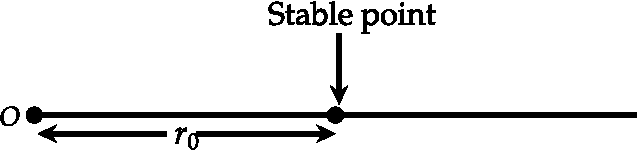
\includegraphics[height=1.5cm,width=6cm]{diagram-20220221(2)-crop}
		\end{figure}
		\begin{align*}
		V_{e f f}=\frac{L^{2}}{2 m r^{2}}+V(r)&=\frac{L^{2}}{2 m r^{2}}-\frac{k}{r}\\
		\text{For stable point (orbit) }\left.\frac{\partial V_{e f f}}{\partial r}\right|_{r=r_{0} .}&=0\\
		\therefore-\frac{L^{2}}{m r_{0}^{3}}+\frac{k}{r_{0}^{2}}&=0 \text { or } r_{0}=\frac{L^{2}}{m k}\\
		\text{	Therefore radius of stable circular orbit is }L^{2} / \mathrm{mk}
		\end{align*}
		Angular frequency of oscillation about stable point:
		\begin{figure}[H]
			\centering
			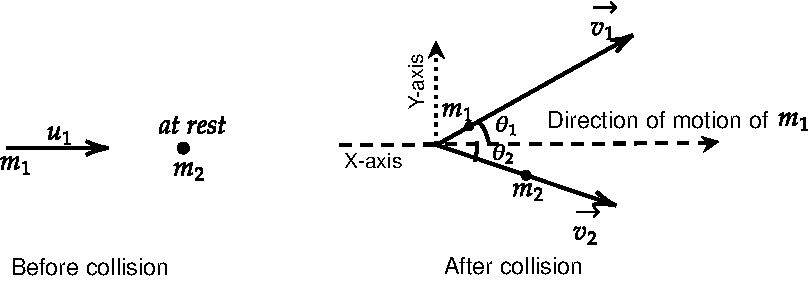
\includegraphics[height=0.7cm,width=6.4cm]{diagram-20220221-crop}
		\end{figure}
		\begin{align*}
		\omega&=\sqrt{\frac{\left.\frac{\partial^{2} V_{e f f}}{\partial r^{2}}\right|_{r=r_{0}}}{m}}=\sqrt{\frac{\left(\frac{3 L^{2}}{m r_{0}^{4}}-\frac{2 k}{r_{0}^{3}}\right)}{m}}\\
		&=\sqrt{\frac{\frac{1}{r_{0}^{3}}\left(\frac{3 L^{2}}{m \cdot \frac{L^{2}}{m k}}-2 k\right)}{m}}=\sqrt{\frac{k}{m r_{0}^{3}}}=\sqrt{\frac{k^{4} m^{2}}{L^{6}}}=\frac{m k^{2}}{L^{3}}
		\end{align*}
		actual radial oscillation is as shown in figure.
		\begin{figure}[H]
			\centering
			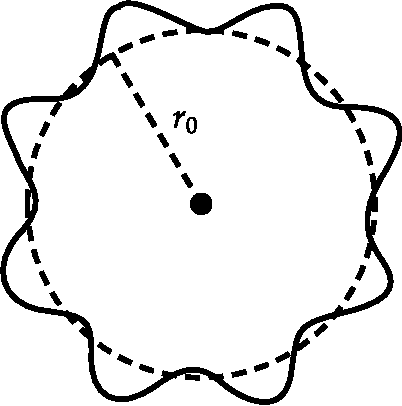
\includegraphics[height=4cm,width=4cm]{diagram-20220221(1)-crop}
		\end{figure}
	\end{answer}
	\item  A small asteroid is approaching a massive star with a speed $v$ from very large distance, at an impact parameter ' $b$ ' as shown in figure. If the mass of the star is $M$ and its radius is $R$, then what is the minimum value of $b$ such that the asteroid will miss the star?
	\begin{answer}
		Angular momentum of asteroid about centre of star is $L=m v b$
		\begin{figure}[H]
			\centering
			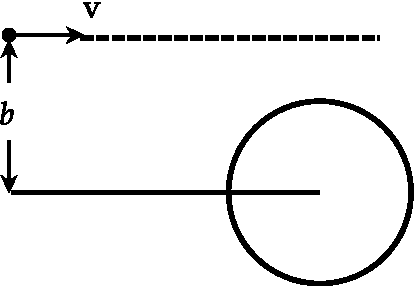
\includegraphics[height=3.5cm,width=5cm]{diagram-20220221(3)-crop}
		\end{figure}
		\begin{align*}
		\text{Effective potential energy }V_{e f f}&=\frac{-G M m}{r}+\frac{L^{2}}{2 m r^{2}}=\frac{-G M m}{r}+\frac{m v^{2} b^{2}}{2 r^{2}}
		\end{align*}
		For minimum value of $b$ we will have to assume that asteroid just misses the star as shown in figure. Equivalent 1-d problem is also shown in figure
		\begin{figure}[H]
			\centering
			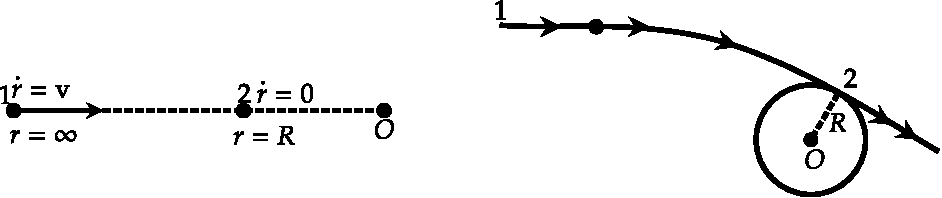
\includegraphics[height=2.5cm,width=12cm]{diagram-20220221(7)-crop}
		\end{figure}
		\text{Total energy is conserved in central force motion }
		\begin{align*}
		\text{Therefore, }E_{1}&=E_{2}\\
		\text{or }&\left(\frac{1}{2} m \dot{r}^{2}+V_{e f f}\right)_{\mathrm{at} r=\infty}=\left(\frac{1}{2} m \dot{r}^{2}+V_{e f f}\right)_{\mathrm{at} r=R}\\
		\frac{1}{2} m v^{2}-\frac{G M m}{\infty}+\frac{m v^{2} b^{2}}{\infty}&=\left(\frac{1}{2} m o^{2}-\frac{G M m}{R}+\frac{m v^{2} b^{2}}{2 R^{2}}\right)\\
		\therefore v^{2}+\frac{2 G M}{R}&=\frac{v^{2} b^{2}}{R^{2}} \quad \text { or } b=R \sqrt{1+\frac{2 G M}{R v^{2}}}
		\end{align*}
	\end{answer}
	\item  A particle is thrown in radially outward direction from earth's surface with initial speed $\sqrt{\frac{3 G M}{4 R}}$ where $M$ is mass of earth $R$ is radius of earth. Find the height upto which particle goes.
	\begin{answer}
		Particle has been thrown radially outward 
		\begin{figure}[H]
			\centering
			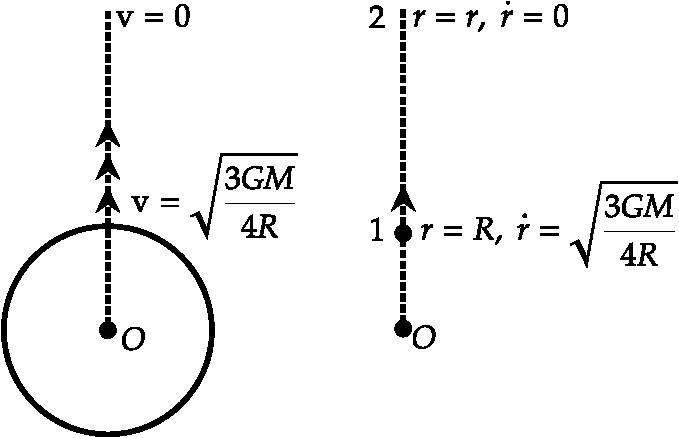
\includegraphics[height=4cm,width=6.5cm]{diagram-20220221(6)-crop}
		\end{figure}
		\begin{align*}
		\text{therefore }L&=0, V_{e f f}=V(r)+\frac{L^{2}}{2 m r^{2}}\\
		\therefore V_{e f f}&=\frac{-G M m}{r}+0\\
		\intertext{from conservation of energy we get }E_{1}&=E_{2}\\
		\text { or }\left(\frac{1}{2} m \dot{r}^{2}+V_{e f f}\right)_{r=R}&=\left(\frac{1}{2} m \dot{r}^{2}+V_{d f}\right)_{r=r} \\
		\frac{1}{2} m \cdot \frac{3 G M}{4 R}-\frac{G M m}{R}&=0-\frac{G M m}{r} \\
		\frac{3}{8 R}-\frac{1}{R}&=-\frac{1}{r} \quad \therefore r=\frac{8 R}{5}
		\end{align*}
		Therefore, maximum height from earth's surface $=r-R=\frac{3 R}{5}$
	\end{answer}
	\item  A particle is thrown from the earth's surface with speed $\sqrt{\frac{G M}{R}}$ where $M=$ mass of earth
	$R=$ radius of earth. If direction of initial velocity makes an angle $\alpha$ with the outward radial direction, find the maximum distance of the particle from centre of earth.
	\begin{answer}
		Angular momentum of the particle is
		\begin{figure}[H]
			\centering
			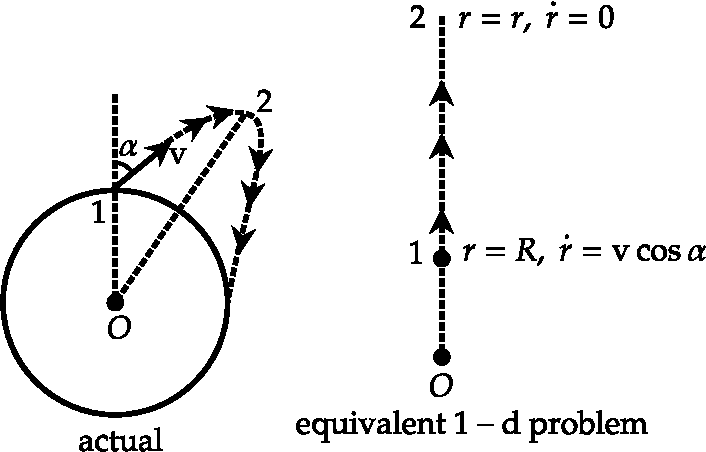
\includegraphics[height=5cm,width=8cm]{diagram-20220221(5)-crop}
		\end{figure}
		\begin{align*}
		L &=m v \sin \alpha R=m \sqrt{\frac{G M}{R}} \sin \alpha R \\
		&=m \sqrt{G M R} \sin \alpha \\
		\therefore V_{e f f} &=V(r)+\frac{L^{2}}{2 m r^{2}}=\frac{-G M m}{r}+\frac{G M m R}{2 r^{2}} \sin ^{2} \alpha
		\end{align*}
		From conservation of energy we get $\mathrm{E}_{1}=\mathrm{E}_{2}$
		\begin{align*}
		\text{	or }\left(\frac{1}{2} m \dot{r}^{2}+V_{e f f}\right)_{r=R}&=\left(\frac{1}{2} m \dot{r}^{2}+V_{e f f}\right)_{r=r}\text{ (see the figure)}\\
		\frac{1}{2} m \frac{G M}{R} \cos ^{2} \alpha-\frac{G M m}{R}+\frac{G M m}{2 R} \sin ^{2} \alpha&=\frac{-G M m}{r}+\frac{G M m R}{2 r^{2}} \sin ^{2} \alpha\\
		\text{Divide both sides by }\frac{G M m}{2 R}\text{ to get }&\cos ^{2} \alpha-2+\sin ^{2} \alpha=-2 \frac{R}{r}+\frac{R^{2}}{r^{2}} \sin ^{2} \alpha\\
		\text{or }-1=-2\left(\frac{R}{r}\right)+\left(\frac{R}{r}\right)^{2} \sin ^{2} \alpha \quad &\therefore\left(\frac{R}{r}\right)^{2} \sin ^{2} \alpha-2\left(\frac{R}{r}\right)+1=0\\
		\therefore \frac{R}{r}=\frac{+2 \pm \sqrt{4-4 \sin ^{2} \alpha}}{2 \sin ^{2} \alpha} \quad \frac{R}{r}&=\frac{+1 \pm \cos \alpha}{\sin ^{2} \alpha} \\
		\therefore r=\frac{R \sin ^{2} \alpha}{1 \pm \cos \alpha}=\frac{R\left(1-\cos ^{2} \alpha\right)}{(1 \pm \cos \alpha)} \quad &\therefore r=R(1-\cos \alpha) \quad \text { or } \quad r=R(1+\cos \alpha)
		\end{align*}
		Since $r$ must be greater than $r$. Therefore, $r=R(1+\cos \alpha)$
	\end{answer}
	\item  A particle moves under a central potential $V(r)=\frac{-k}{r^{m}} .$ What should be value of $m$ for its orbit to be stable.
	\begin{answer}
		\begin{align*}
		\text{Corresponding is }f(r)&=-\frac{\partial V}{\partial r}=\frac{-m k}{r^{m+1}}=-m k r^{-(m+1)}\\
		\text{	We know that for }f&=-k r^{n}\text{ condition for stability is $n>-3$.} 
		\intertext{Therefore for orbit to be stable under given potential we must have.}
		-(m+1)>-3&\text{ or }m+1<3 \quad \therefore m<2
		\end{align*}
	\end{answer}
\end{enumerate}
\section{Lagrangian}
\begin{enumerate}
	\item The Lagrangian of a particle of charge e and mass $m$ in applied electric and magnetic fields is given by $L=\frac{1}{2} \mathrm{~m} \vec{v}^{2}+\mathrm{e} \overrightarrow{\mathrm{A}} \cdot \vec{v}-\mathrm{e} \phi$, where $\overrightarrow{\mathrm{A}}$ and $\phi$ are the vector and scalar potentials corresponding to the magnetic and electric fields, respectively. Which of the following statements is correct?
	 \begin{tasks}(1)
		\task[\textbf{a.}] The carionically conjugate momentum of the particle is given by $\overrightarrow{\mathrm{p}}=\mathrm{m} \overrightarrow{\mathrm{v}}$
		\task[\textbf{b.}]The Hamiltonian of the particle is given by $\mathrm{H}=\frac{\overrightarrow{\mathrm{p}}^{2}}{2 \mathrm{~m}}+\frac{\mathrm{e}}{\mathrm{m}} \cdot \overrightarrow{\mathrm{A}} \cdot \overrightarrow{\mathrm{p}}+\mathrm{e} \phi$
		\task[\textbf{c.}]L remains unchanged under a gauge transformation of the potentials.
		\task[\textbf{d.}]  Under a gauge transformation of the potentials, $\mathrm{L}$ changes by the total time derivative of a function of $\overrightarrow{\mathrm{r}}$ and $\mathrm{t}$.
	\end{tasks}
	\begin{answer}
		\begin{align*}
		\mathrm{L}&=\frac{1}{2} \mathrm{~m} \overrightarrow{\mathrm{v}}-\mathrm{e} \phi+\mathrm{e} \overrightarrow{\mathrm{A}} \cdot \overrightarrow{\mathrm{v}}
	\intertext{	We know that $\vec{E}$ and $\vec{B}$ fields are in variant under gauge transformation.}
		\overrightarrow{\mathrm{A}}(\overrightarrow{\mathrm{x}}, \mathrm{t}) \rightarrow \overrightarrow{\mathrm{A}}^{\prime}&=\overrightarrow{\mathrm{A}}+\vec{\nabla} \lambda(\overrightarrow{\mathrm{x}}, \mathrm{t}) ; \quad \varphi(\overrightarrow{\mathrm{x}}, \mathrm{t}) \rightarrow \varphi^{\prime}=\varphi-\frac{\partial \lambda}{\partial \mathrm{t}}(\overrightarrow{\mathrm{x}}, \mathrm{t})
	\intertext{	where $\lambda(\vec{x}, t)$ is an arbitrary scalar function.}
		\therefore \quad \mathrm{L} \rightarrow \mathrm{L}^{\prime}&=\mathrm{L}+\mathrm{e}\left(\frac{\partial \lambda}{\partial \mathrm{t}}(\overrightarrow{\mathrm{x}}, \mathrm{t})+\overrightarrow{\mathrm{v}} \cdot \vec{\nabla} \lambda(\overrightarrow{\mathrm{x}}, \mathrm{t})\right)
		\end{align*}
		The expression in bracket is just the total time derivative of $\lambda(\vec{x}, t)$.\\
		If we add a total time derivative of a function of $\overrightarrow{\mathrm{x}}$ and $\mathrm{t}$ to the Lagrangian, the equations of motion do not change.\\
		Correct answer is option \textbf{(d)}
	\end{answer}
	\item The Hamiltonian o fa system with $n$ degrees of freedom is given by \\$H\left(q_{i}, \ldots \ldots \ldots ., q_{n} ; p_{i}, \ldots \ldots \ldots \ldots, p_{n} ; t\right)$\\
	with an explicit dependence on the time $t$. Which of the following is correct?
	 \begin{tasks}(1)
		\task[\textbf{a.}]Different phase trajectories cannot intersect each other
		\task[\textbf{b.}]H always represents the total energy of the system and is a constant of the motion.
		\task[\textbf{c.}]The equations $\dot{\mathrm{q}}_{\mathrm{i}}=\partial \mathrm{H} / \partial \mathrm{p}_{\mathrm{i}}, \dot{\mathrm{p}}_{\mathrm{i}}=-\partial \mathrm{H} / \partial \mathrm{q}_{\mathrm{i}}$ are not valid since H has explicit time dependence.
		\task[\textbf{d.}] Any initial volume element in phase space remains unchanged in magnitude under time evolution.
	\end{tasks}
\begin{answer}
	According to Liouville's theorem, the phase volume occupied by a collection of system evolve according to - Hamilton's equation of motion, and will be preserved in time.\\
	Correct answer is option \textbf{(d)}
\end{answer}
	\item A double pendulum consists of two point masses $m$ attached by massless strings of length $l$ as shown in the figure:
	\begin{figure}[H]
		\centering
		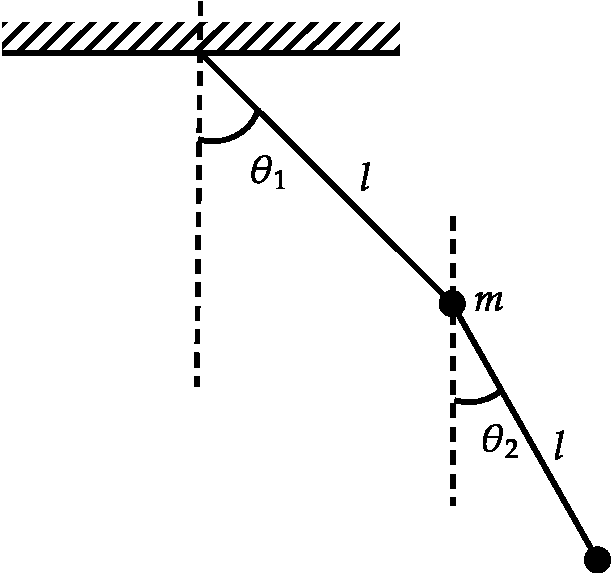
\includegraphics[height=4cm,width=4.5cm]{CM-02}
	\end{figure}
	The kinetic energy of the pendulum is :
	 \begin{tasks}(2)
		\task[\textbf{a.}]$\frac{1}{2} \mathrm{~m} \ell^{2}\left[\dot{\theta}_{1}^{2}+\dot{\theta}_{2}^{2}\right]$
		\task[\textbf{b.}]$\frac{1}{2} m \ell^{2}\left[2 \dot{\theta}_{1}^{2}+\dot{\theta}_{2}^{2}+2 \dot{\theta}_{1} \dot{\theta}_{2} \cos \left(\dot{\theta}_{1}-\dot{\theta}_{2}\right)\right]$
		\task[\textbf{c.}]$\frac{1}{2} m \ell^{2}\left[\dot{\theta}_{1}^{2}+2 \dot{\theta}_{2}^{2}+2 \dot{\theta}_{1} \dot{\theta}_{2} \cos \left(\dot{\theta}_{1}-\dot{\theta}_{2}\right)\right]$
		\task[\textbf{d.}] $\frac{1}{2} \mathrm{~m} \ell^{2}\left[2 \dot{\theta}_{1}^{2}+\dot{\theta}_{2}^{2}+2 \dot{\theta}_{1} \dot{\theta}_{2} \cos \left(\dot{\theta}_{1}+\dot{\theta}_{2}\right)\right]$
	\end{tasks}
	\begin{answer}
		\begin{align*}
	\mathrm{x}_{1}&=\ell \sin \theta_{1},  \mathrm{x}_{2}=\ell \sin \theta_{1}+\ell \sin \theta_{2} \\ \mathrm{y}_{1}&=-\ell \cos \theta_{1},  \mathrm{y}_{2}=-\ell \cos \theta_{1}-\ell \cos \theta_{2} \\ \dot{\mathrm{x}}_{1}&=\ell \cos \theta_{1} \dot{\theta}_{1},  \dot{\mathrm{y}}_{1}=\ell \sin \theta_{1} \dot{\theta}_{1}
		\end{align*}
		\begin{figure}[H]
			\centering
			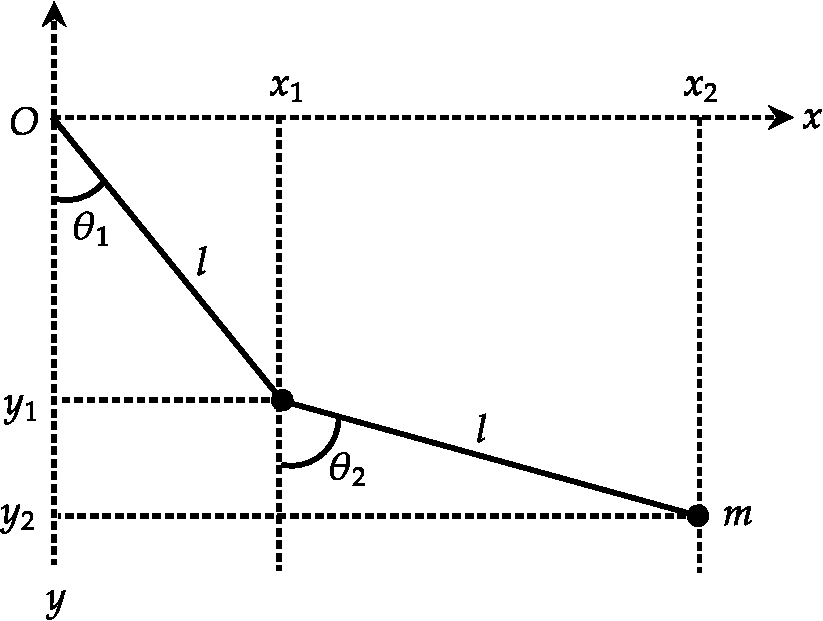
\includegraphics[height=4.5cm,width=6.5cm]{CM-03}
		\end{figure}
		\begin{align*}
		\dot{x}_{2}&=\ell \cos \theta_{1} \dot{\theta}_{1}+\ell \cos \theta_{2} \dot{\theta}_{2} ; \quad \dot{y}_{2}=\ell \sin \theta_{1} \dot{\theta}_{1}+\ell \sin \theta_{2} \dot{\theta}_{2},\\
		T&=\frac{m}{2}\left(\dot{x}_{1}^{2}+\dot{y}_{1}^{2}\right)+\frac{m}{2}\left(\dot{x}_{2}^{2}+\dot{y}_{2}^{2}\right)\\
		&=\frac{\mathrm{m}}{2} \dot{\theta}_{1}^{2} \ell^{2}+\frac{\mathrm{m}}{2}\left[\dot{\theta}_{1}^{2} \ell^{2}+\dot{\theta}_{2}^{2} \ell^{2}+2 \ell^{2} \dot{\theta}_{1} \dot{\theta}_{2} \cos \left(\theta_{1}-\theta_{2}\right)\right]\\
		&=\frac{\mathrm{m} \ell^{2}}{2}\left[2 \dot{\theta}_{1}^{2}+\dot{\theta}_{2}^{2}+2 \dot{\theta}_{1} \dot{\theta}_{2} \cos \left(\theta_{1}-\theta_{2}\right)\right]
		\end{align*}
		Correct answer is \textbf{(b)}
	\end{answer}
	\item A particle of mass ' $\mathrm{m}$ ' moves inside a bowl. If the surface of the bowl is given by the equation $\mathrm{z}=\frac{1}{2} \mathrm{a}\left(\mathrm{x}^{2}+\mathrm{y}^{2}\right)$, where $a$ is a constant, the Lagrangian of the particle is:
	 \begin{tasks}(2)
		\task[\textbf{a.}] $\frac{1}{2} m\left(\dot{r}^{2}+r^{2} \dot{\phi}^{2}-g a r^{2}\right)$
		\task[\textbf{b.}] $\frac{1}{2} m\left[\left(1+a^{2} r^{2}\right) \dot{r}^{2}+r^{2} \dot{\phi}^{2}\right]$
		\task[\textbf{c.}]$\frac{1}{2} m\left(\dot{r}^{2}+r^{2} \dot{\theta}^{2}+r^{2} \sin ^{2} \dot{\phi}^{2}-g a r^{2}\right)$
		\task[\textbf{d.}]  $\frac{1}{2} m\left[\left(1+a^{2} r^{2}\right) \dot{r}^{2}+r^{2} \dot{\phi}^{2}-g a r^{2}\right]$
	\end{tasks}
	\begin{answer}$\left. \right. $
		\begin{figure}[H]
			\centering
			
\includegraphics[height=1.5cm,width=2cm]{CM-04}
		\end{figure}
		\begin{align*}
		z&=\frac{1}{2} a\left(x^{2}+y^{2}\right)=\frac{1}{2} a r^{2} \quad \Rightarrow \dot{z}=a r \dot{r}\\
	\text{	K.E. }&=T=\frac{1}{2} m\left(\dot{x}^{2}+\dot{y}^{2}+\dot{z}^{2}\right)\\
	&=\frac{1}{2} m\left(\dot{r}^{2}+r^{2} \dot{\varphi}^{2}+\dot{z}^{2}\right)\\
	&=\frac{1}{2} m\left(\dot{r}^{2}+r^{2} \dot{\varphi}^{2}+a^{2} r^{2} \dot{r}^{2}\right) \qquad\text{ P.E.} =V=m g z=\frac{1}{2} m g a r^{2}\\
	L&=T-V=\frac{1}{2} m\left(\dot{r}^{2}+r^{2} \dot{\varphi}^{2}+a^{2} r^{2} \dot{r}^{2}-g a r^{2}\right)=\frac{1}{2} m\left[\left(1+a^{2} r^{2}\right) r^{2}+r^{2} \dot{\varphi}^{2}-g a r^{2}\right]
		\end{align*}
		Correct answer is option\textbf{(d)}
	\end{answer}
	\item A mass point glides without friction on a cycloid, which is given by $x=a(\vartheta-\sin \vartheta)$ and $y=a(1+\cos \vartheta)$ (with $0 \leq \vartheta \leq 2 \pi$ ). Determine\\
	(a) the Lagrangian, and\\
	(b) the equation of motion\\
	(c) Solve the equation of motion
	\begin{answer}
		The cycloid is represented by
		\begin{align*}
		x=a(\vartheta-\sin \vartheta), \quad y=a(1+\cos \vartheta),
		\end{align*}
		\begin{figure}[H]
			\centering
			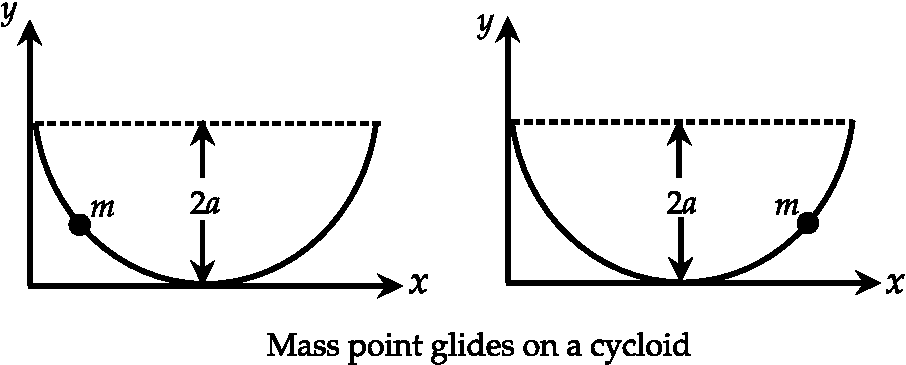
\includegraphics[height=3.2cm,width=9cm]{CM-05}
		\end{figure}
		\begin{align*}
	\text{	where }&0 \leq \vartheta \leq 2 \pi.\text{ The kinetic energy is}\\
		T=\frac{1}{2} m\left(\dot{x}^{2}+\dot{y}^{2}\right)&=\frac{1}{2} m a^{2}\left\{[(1-\cos \vartheta) \dot{\vartheta}]^{2}+[-(\sin \vartheta) \dot{\vartheta}]^{2}\right\},\\
	\text{	and the potential energy is }V&=m g y=m g a(1+\cos \vartheta).\\
		\text{The Lagrangian is given by }L&=T-V=m a^{2}(1-\cos \vartheta) \dot{\vartheta}^{2}-m g a(1+\cos \vartheta).\\
		\text{The equation of motion then reads }&\frac{d}{d t}\left(\frac{\partial L}{\partial \dot{\vartheta}}\right)-\frac{\partial L}{\partial \vartheta}=0,\\
	\text{	i.e., }\quad &\frac{d}{d t}\left[2 m a^{2}(1-\cos \vartheta) \dot{\vartheta}\right]-\left[m a^{2}(\sin \vartheta) \dot{\vartheta}^{2}+m g a \sin \vartheta\right]=0\\
	\text{ or }\quad &\frac{d}{d t}[(1-\cos \vartheta) \dot{\vartheta}]-\frac{1}{2}(\sin \vartheta) \dot{\vartheta}^{2}-\frac{8}{2 a} \sin \vartheta=0,\\
	\text{ i.e.,} \quad&(1-\cos \vartheta) \ddot{\vartheta}+\frac{1}{2}(\sin \vartheta) \dot{\vartheta}^{2}-\frac{g}{2 a} \sin \vartheta=0.\\
\text{	By setting }u&=\cos \left(\frac{\vartheta}{2}\right), \text{one has }\frac{d u}{d t}=-\frac{1}{2} \sin \left(\frac{\vartheta}{2}\right) \dot{\vartheta}\text{ and } \frac{d^{2} u}{d t^{2}}\\&=-\frac{1}{2} \sin \left(\frac{\vartheta}{2}\right) \ddot{\vartheta}-\frac{1}{4} \cos \left(\frac{\vartheta}{2}\right) \dot{\vartheta}^{2} .\\ \text{Since }&\cot \left(\frac{\vartheta}{2}\right)=\sin \frac{\vartheta}{(1-\cos \vartheta)},\text{ we can write as}\\
\ddot{\vartheta}+\frac{1}{2} \cot \left(\frac{\vartheta}{2}\right) \dot{\vartheta}^{2}-\frac{g}{2 a} \cot \left(\frac{\vartheta}{2}\right)&=0,\text{ and therefore,} \frac{d^{2} u}{d t^{2}}+\frac{g}{4 a} u=0. 
\intertext{The solution of this differential equation is}
u&=\cos \left(\frac{\vartheta}{2}\right)=C_{1} \cos \sqrt{\frac{g}{4 a}} t+C_{2} \sin \sqrt{\frac{g}{4 a}} t 
\intertext{ The motion is just like the vibration of an ordinary pendulum of length $l=4 a$. The arrangement is therefore called a "cycloid pendulum".}
		\end{align*}
	\end{answer}
	\item 	Three particles of equal mass ' $m$ ' are connected by two identical massless springs of stiffiness constant ' $k$ ' as shown in the figure.\\
	If $x_{1}, x_{2}$ and $x_{3}$ denote the displacements of the masses from their respective equilibrium positions, the potential energy of the system is:
	 \begin{tasks}(2)
		\task[\textbf{a.}]$\frac{1}{2} k\left(x_{1}^{2}+x_{2}^{2}+x_{3}^{2}\right)$
		\task[\textbf{b.}]$\frac{1}{2} k\left[x_{1}^{2}+x_{2}^{2}+x_{3}^{2}-x_{2}\left(x_{1}+x_{3}\right)\right]$
		\task[\textbf{c.}]$\frac{1}{2} k\left[x_{1}^{2}+2 x_{2}^{2}+x_{3}^{2}+2 x_{2}\left(x_{1}+x_{3}\right)\right]$
		\task[\textbf{d.}] $\frac{1}{2} k\left[x_{1}^{2}+2 x_{2}^{2}+x_{3}^{2}-2 x_{2}\left(x_{1}+x_{3}\right)\right]$
	\end{tasks}
	\begin{answer}
		\begin{align*}
		\text{Potential energy }&=\frac{1}{2} k\left(x_{2}-x_{1}\right)^{2}\hspace{2cm}
		\text{first spring}\\
	\text{	Potential energy }&=\frac{1}{2} k\left(x_{3}-x_{2}\right)^{2}\hspace{2cm}
	\text{	second spring}
	\intertext{Potential energy of the system,}
	&=\frac{1}{2} k\left(x_{2}-x_{1}\right)^{2}+\frac{1}{2} k\left(x_{3}-x_{2}\right)^{2}=\frac{1}{2} k\left[x_{1}^{2}+x_{2}^{2}-2 x_{1} x_{2}+x_{2}^{2}+x_{3}^{2}-2 x_{2} x_{3}\right]\\
	&=\frac{1}{2} k\left[x_{1}^{2}+2 x_{2}^{2}+x_{3}^{2}-2 x_{2}\left(x_{1}+x_{3}\right)\right]
		\end{align*}
		Correct answer is option \textbf{(d)}
	\end{answer}
	\item The Lagrangian of a particle of mass $m$ moving in one dimensions is given by
	$$
	\mathrm{L}=\frac{1}{2} \mathrm{~m} \dot{\mathrm{x}}^{2}-\mathrm{bx}
	$$
	where $b$ is a positive constant. The coordinate of the particle $x(t)$ at time $t$ is given by: (in the following $c_{1}$ and $c_{2}$ are constants)
	 \begin{tasks}(2)
		\task[\textbf{a.}]$-\frac{b}{2 m} t^{2}+c_{1} t+c_{2}$
		\task[\textbf{b.}]$c_{1} t+c_{2}$
		\task[\textbf{c.}]$c_{1} \cos \left(\frac{b t}{m}\right)+c_{2} \sin \left(\frac{b t}{m}\right)$
		\task[\textbf{d.}] $c_{1} \cosh \left(\frac{b t}{m}\right)+c_{2} \sin h\left(\frac{b t}{m}\right)$
	\end{tasks}
	\begin{answer}
		\begin{align*}
		L&=\frac{1}{2} m \dot{x}^{2}-b x=\mathrm{T}-\mathrm{V}\\
		\therefore \mathrm{V}&=b x
		\intertext{ This is same as uniform gravitational potential. Therefore, solution must be of the form. This is same as uniform} \mathrm{S}&=\mathrm{S}_{0}+\mathrm{ut}+\frac{1}{2} \mathrm{at}^{2}
		\end{align*}
		Correct answer is option \textbf{(a)}
	\end{answer}
	\item A particle moves in a potential $V=x^{2}+y^{2}+\frac{z^{2}}{2}$. Which component (s) of the angular momentum is $/$ are constant (s) of motion?
	 \begin{tasks}(2)
		\task[\textbf{a.}]None
		\task[\textbf{b.}]$L_{x}, L_{y}$ and $L_{z}$
		\task[\textbf{c.}]Only $L_{x}$ and $L_{y}$
		\task[\textbf{d.}] Only $\mathrm{L}_{z}$
	\end{tasks}
	\begin{answer}
		\begin{align*}
		\text{Given }V(x, y, z)&=x^{2}+y^{2}+\frac{z^{2}}{2}
	\intertext{	In polar co-ordinate (spherical polar)}
	V&=r^{2} \sin ^{2} \theta+\frac{r^{2} \cos ^{2} \theta}{2} \quad\left[\begin{array}{l}x=r \cos \phi \sin \theta \\ y=r \sin \phi \sin \theta \\ z=r \cos \theta\end{array}\right.
\intertext{	Therefore, Lagrangian of system is}
	\mathrm{L}&=\mathrm{T}-\mathrm{V} \\
	L&=\frac{1}{2} m\left(\dot{r}^{2}+r^{2} \dot{\theta}^{2}+r^{2} \sin ^{2} \theta \dot{\phi}^{2}\right)-r^{2} \sin ^{2} \theta-\frac{r^{2} \cos ^{2} \theta}{2}
		\end{align*}
		$\phi$ is cyclic, therefore $p_{\phi}$ is constant of motion.\\
		$p_{\phi}$ is equal to $L_{z}$. Therefore, $L_{z}$ is constant of motion.\\
		Correct answer is option \textbf{(d)}
	\end{answer}
	\item	A particle of mass $m$ is projected with an initial velocity $u$ at an angle $\alpha$ with the horizontal. Use Lagran equations to describe the motion of projectile. The resistance of air is negligible.
	\begin{answer}
			Let $x, y$ be the coordinate of the particle at any instant. The system is holonomic because its positic confined to a plane and conservative because the only external force acting on the projectile is conse tive.
		\begin{align*}
		T&=\frac{1}{2} m\left(\dot{x}^{2}+\dot{y}^{2}\right)\text{ and }V=m g y\\
		\therefore L&=T-V=\frac{1}{2} m\left(\dot{x}^{2}+\dot{y}^{2}\right)-m g v\\
		\frac{\partial L}{\partial \dot{x}}&=m \dot{x}\text{ and } \frac{\partial L}{\partial x}=0\\
		\text{By Lagrange's equation, }\frac{d}{d t}\left(\frac{\partial L}{\partial \dot{x}}\right)&=\frac{\partial L}{\partial x}\\
		\therefore \quad \frac{d}{d t}(m \dot{x})&=0 \text { or } \ddot{x} =0 \\
		\frac{\partial L}{\partial \dot{y}}&=m y \text { and } \frac{\partial L}{\partial y} =-m g\\
		\text{By Lagrange's equation }\frac{d}{d t}\left(\frac{\partial L}{\partial \dot{y}}\right)&=\frac{\partial L}{\partial y}\\
		 \therefore \quad \frac{d}{d t}(m y)&=-m g\text{ or }\ddot{y}=-g
		 \intertext{Thus, $\ddot{x}=0, \ddot{y}=-g$ are the two equations describing the motion of a projectile. Proceeding with the first equation,}
		 \frac{d}{d t}\left(\frac{d x}{d t}\right)&=0 \text { or } d\left(\frac{d x}{d t}\right)=0\\
		 \text{Integrating, }\quad \frac{d x}{d t}&=c_{1}(\text{ a constant} )\\
		\text{ At }t&=0, \quad \frac{d x}{d t}=u \cos \alpha ; \quad \therefore u \cos \alpha=c_{1}\\
		\therefore \quad \frac{d x}{d t}&=u \cos \alpha, \quad \text { or } d x=u \cos \alpha d t\\
	\text{	Integrating, }x&=(u \cos \alpha) t+x_{0}(\text{ a constant })\\
\text{	At $t=0, x=0$, }&\text{therefore, }x_{0}=0 ; x=(u \cos \alpha) t
 \intertext{Proceeding with the second equation,}
	\frac{d}{d t}\left(\frac{d y}{d t}\right)&=-g, \text { or } d\left(\frac{d y}{d t}\right)=-g d t\\
\text{	Integrating, }\frac{d y}{d t}&=-g t+c_{2}(\mathrm{a}\text{ constant })\\
	\text{At }t&=0, \frac{d y}{d t}=u \sin \alpha ; \therefore u \sin \alpha=c_{2}\\
	\therefore \quad \frac{d y}{d t}&=-g t+u \sin \alpha, o r d y=-g t d t+u \sin \alpha d t\\
\text{	Integrating, }y&=-\frac{1}{2} g t^{2}+(u \sin \alpha) t+y_{0}\\
\text{	At }t&=0, y=0\text{ and therefore, $y_{0}=0$}\\
	\therefore \quad y&=(u \sin \alpha) t-\frac{1}{2} g t^{2}
		\end{align*}
		Thus, $x=(u \cos \alpha) t, y=(u \sin \alpha) t-\frac{1}{2} g t^{2}$ are the two solved equation describing the motion of a projectile.
	\end{answer}
	\item A particle of mass $m$ is moving in a plane under the influence of a force directed towards a fixed point and varying inversely as the square of the distance from that point. Set up the Lagrangian and equations of motion of the particle.
	\begin{answer}
		The problem is best solved in polar coordinates with respect to the fixed point as origin and any line through it as the reference line. Let $(r, \theta)$ be the polar coordinates of the particle at any time. Since there are two coordinates there will be two Lagrange's equations describing the motion of the particle. Motion is holonomic because the position of the particle is confined to a plane and conservative because the force is derivable from energy or energy is derivable from the force.
		\begin{figure}[H]
			\centering
			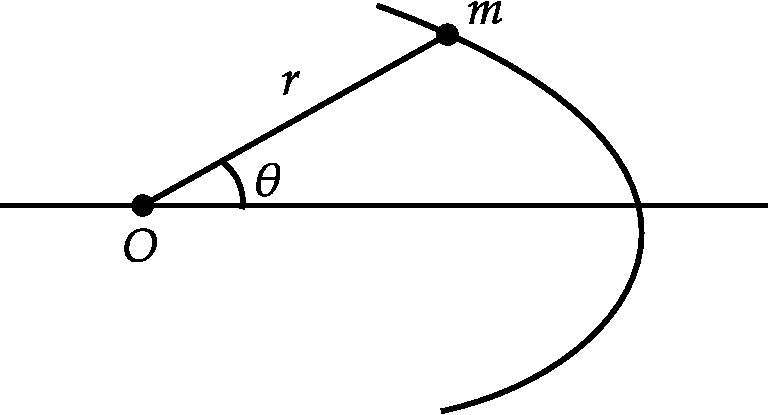
\includegraphics[height=2.5cm,width=5cm]{CM-06}
		\end{figure}
		\begin{align*}
		T&=\frac{1}{2} m \dot{r}^{2} \text{(linear kinetic energy)} +\frac{1}{2} I \dot{\theta}^{2} \text{(rotational $k$. energy)}\\
		\text{Or, }\quad T&=\frac{1}{2} m \dot{r}^{2}+\frac{1}{2}\left(m r^{2}\right) \dot{\theta}^{2} \quad\left(\because I=m r^{2}\right)
		\intertext{Since force varies inversely as the square of the distance and it is directed towards the origin, $F=-\left(k / r^{2}\right)$ where $k$ is a constant. But}
		F&=-\left(\frac{d V}{d r}\right)\\
		\therefore\quad&=\frac{k}{r^{2}}=-\frac{d V}{d r}\text{, or } d V=\frac{k d r}{r^{2}}\\
		\text{Integrating, }V&=-\frac{k}{r}+V_{0}\text{ (a constant)}\\
		\text{At }r&=\infty, V=0\text{ and therefore, }V_{0}=0 ; \therefore V=-\left(\frac{k}{r}\right)\\
		\therefore \quad L&=T-V=\frac{1}{2} m\left(\dot{r}^{2}+r^{2} \dot{\theta}^{2}\right)+\frac{k}{r}\\
		\frac{\partial L}{\partial \dot{r}}&=m \dot{r}\text{ and }\frac{\partial L}{\partial r}=m r \dot{\theta}^{2}-\frac{k}{r^{2}}\\
		\frac{\partial L}{\partial \dot{\theta}}&=m r^{2} \dot{\theta}\text{ and} \frac{\partial L}{\partial \theta}=0\\
		\text{By Lagrange's equations of motion, }&\left[\frac{d}{d t}\left(\frac{\partial L}{\partial q_{k}}\right)=\frac{\partial L}{\partial q_{k}}\right]\text{ we have }\\
		\frac{d}{d t}(m \dot{r})&=m r \dot{\theta}^{2}-\frac{k}{r^{2}}\text{ and } \frac{d}{d t}\left(m r^{2} \dot{\theta}\right)=0\\
		\text{Or, }\quad \ddot{r}&=r \dot{\theta}^{2}-\frac{k}{m r^{2}}\text{ and} r^{2} \dot{\theta}=\text{ constant}\\
	\text{	Or, }\quad \ddot{r}-r \dot{\theta}^{2}&=-\frac{k}{m r^{2}}\text{ or }\ddot{r}-r \dot{\theta}^{2}=-\frac{\omega^{2}}{r^{2}}\\
\text{	where, }\omega^{2}&=\frac{k}{m}\text{ and }r^{2} \dot{\theta}=h \text{(another constant).}
\intertext{	Thus equations describing the motion of the particles are} \ddot{r}-r \dot{\theta}^{2}&=-\frac{\omega^{2}}{r^{2}}\text{ and }r^{2} \dot{\theta}=h\text{ where }\omega^{2}\text{ and $h$ are constants.}
		\end{align*}
	\end{answer}
	\item Obtain the Lagrangian of a linear simple harmonic oscillator and the equation of motion in one dimension.
	\begin{answer}
		In a simple harmonic oscillator the particle is acted on by a force which is directed towards a fixed point (position of equilibrium) and whose magnitude varies linearly with the distance from the position ofequilibrium. That is, $F=-k x$ where $\mathrm{x}$ is the distance of the particle from the equilibrium position.
		\begin{align*}
		\text{But}
		F&=-\left(\frac{d V}{d x}\right) ; \quad \because d V=-F d x=h x d x\\
		\text{Integrating, }\quad V&=\frac{1}{2} k x^{2}+V_{0}(a\text{ constant })\\
	\text{	At }x=0, V&=0\text{ and therefore, }V_{0}=0\\
		\therefore \quad V&=\frac{1}{2} k x^{2} ; \quad T=\frac{1}{2} m \dot{x}^{2}\\
		\therefore \quad L&=T-V=\frac{1}{2} m x^{2}-\frac{1}{2} k x^{2}\\
	\text{	Now, }\quad \frac{\partial L}{\partial \dot{x}}&=m \dot{x}\text{ and } \frac{\partial L}{\partial \dot{x}}=-k x\\
		\text{By Lagrange's equation, }&\frac{d}{d t}\left(\frac{\partial L}{\partial \dot{x}}\right)=\frac{\partial L}{\partial x}\\
		\therefore\quad\frac{d}{d t}(m x)&=-k x, \text { or } m \ddot{x}=-k x
		\intertext{This is the equation of a simple harmonic oscillator in one dimension.}
		\end{align*}
	\end{answer}
	\item Figure below shows a solid cylinder with centre $G$ and radius $a$ rolling on the rough inside surface of a fixed cylinder with centre $O$ and radius $b>a$. Find the Lagrange equation of motion and deduce the period of small oscillations about the equilibrium position.
	\begin{figure}[H]
		\centering
		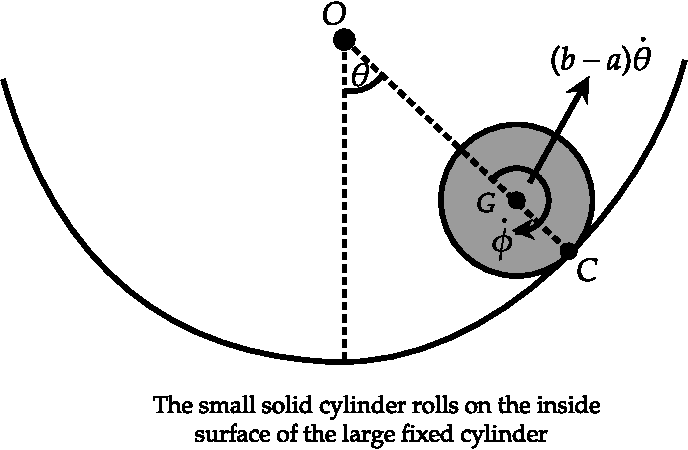
\includegraphics[height=4cm,width=7cm]{Lagrangian 01}
	\end{figure}
	\begin{answer}
		If the cylinder were not obliged to roll, the system would have two degrees of freedom with generalised coordinates $\theta$ (the angle between $O G$ and the downward vertical) and $\phi$ (the rotation angle of the cylinder measured from some reference position).\\
		The roling condition imposes the kinematical constraint.
		\begin{align*}
		(b-a) \dot{\theta}-a \dot{\phi}&=o
	\intertext{	This constraint is integrable and is equivalent to the geometrical constraint.}
	(b-a) \theta-a \phi&=o
\intertext{	on taking $\phi=0$ when $\theta=0$. Thus the rolling cylinder is a standard conservative system with one degree of freedom.}
\intertext{Take $\theta$ as the generalised coordinate. Then the kinetic energy is given by}
T &=\frac{1}{2} m((b-a) \dot{\theta})^{2}+\frac{1}{2}\left(\frac{1}{2} m a^{2}\right) \dot{\phi}^{2} \\
&=\frac{1}{2} m((b-a) \dot{\theta})^{2}+\frac{1}{2}\left(\frac{1}{2} m a^{2}\right)\left(\frac{b-a}{a}\right)^{2} \dot{\theta}=\frac{3}{4} m(b-a)^{2} \dot{\theta}^{2}\\
\text{and the potential energy by }V&=-m g(b-a) \cos \theta
\intertext{There is only one Lagrange equation, namely}
\frac{d}{d t}\left[\frac{3}{2} m(b-a)^{2} \dot{\theta}\right]-0*=-m g(b-a) \sin \theta
\intertext{which simplifies to give}
\ddot{\theta}+\frac{2 g}{3(b-a)} \sin \theta&=0
\intertext{Interestingly, this equation is identical to the exact equation for the oscillations of a simple pendulum of length $3(b-a) / 2$ as obtaind.}
\intertext{The linearised equation governing small oscillations of the cylinder about $\theta=0$ is is}
\ddot{\theta}+\frac{2 g}{3(b-a)} \theta&=0
\intertext{so that the period $\tau$ of small oscillation is given by}
\tau&=2 \pi\left(\frac{3(b-a)}{2 g}\right)^{1 / 2}
		\end{align*}
\end{answer}
\item A pendulum of mass $m$ is attached to a block of mass $M$. The block slides on a horizontal frictionless surface. Find the Lagrangian and equation of motion of the pendulum. For small amplitude oscillations, derive an expression for periodic time.
\begin{figure}[H]
	\centering
	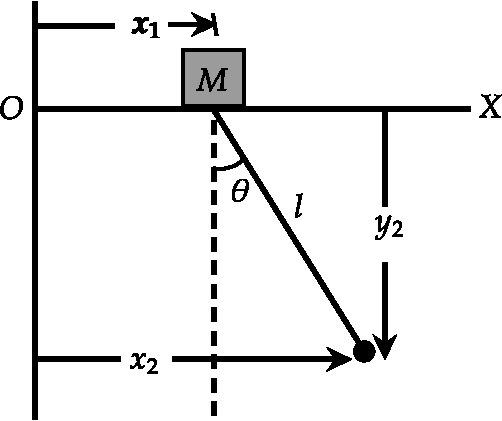
\includegraphics[height=4cm,width=5cm]{Lagrangian 02}
\end{figure}
\begin{answer}
		Let at any time $t$ the coordinates of $M$ and $m$ be $\left(x_{1}, 0\right)$ and $\left(x_{2}, y_{2}\right)$ respectively.
	\begin{align}
	\text{Here, }\quad x_{2}&=x_{1}+\ell \sin \theta\text{ and }ay_{2}=-\ell \cos \theta.\text{ The suitable generalized coordinates are $x_{1}$ and $\theta$.}\notag\\
	 T &=\frac{1}{2} M \dot{x}_{1}^{2}+\frac{1}{2} m\left(\dot{x}_{2}^{2}+\dot{y}_{2}^{2}\right) \notag\\ &=\frac{1}{2} M \dot{x}_{1}^{2}+\frac{1}{2} m\left[\left(\dot{x}_{1}+\ell \dot{\theta} \cos \theta\right)^{2}+(\ell \dot{\theta} \sin \theta)^{2}\right] \notag\\ &=\frac{1}{2} M \dot{x}_{1}^{2}+\frac{1}{2} m\left(\dot{x}_{1}^{2}+\ell^{2} \dot{\theta}^{2}+2 \ell \dot{x}_{1} \dot{\theta} \cos \theta\right)\notag\\
	 (\text{because }\dot{x}_{2}&=\dot{x}_{1}+\ell \cos \theta \dot{\theta} \text{and }\dot{y}_{2}=\ell \sin \theta \dot{\theta} )\notag\\
	 V&=-m g \cos \theta\notag\\
	\text{ Hence, }\quad L&=T-V=\frac{1}{2}(M+m) \dot{x}_{1}^{2}+\frac{1}{2} m \ell^{2} \dot{\theta}^{2}+m \ell \dot{x}_{1} \dot{\theta} \cos \theta+m g \ell \cos \theta\notag
	\intertext{We see that $x_{1}$ is cyclic coordinate, so}\notag
	\text{Here, }\frac{\partial L}{\partial x_{1}}&=0\text{ and }\frac{\partial L}{\partial \dot{x}_{1}}=(M+m) \dot{x}_{1}+m \ell \dot{\theta} \cos \theta\text{ is conserved.}\notag\\
	\frac{\partial L}{\partial \theta}&=m \ell\left(\dot{x}_{1} \dot{\theta}+g\right)(-\sin \theta) \text { and } \frac{\partial L}{\partial \dot{\theta}}=m \ell^{2} \dot{\theta}+m \ell \dot{x}_{1} \cos \theta\notag
\intertext{	Equation of motion in $\theta$ is}\notag
	m \ell^{2} \ddot{\theta}&+m \ell \ddot{x}_{1} \cos \theta+m \ell(-\sin \theta) \dot{\theta} \dot{x}_{1}-m \ell(-\sin \theta) \dot{x}_{1} \dot{\theta}+m g \ell \sin \theta=0\notag\\
\text{	Or, }\quad m \ell^{2} \ddot{\theta}&+m \ell \cos \theta \ddot{x}_{1}+m g \ell \sin \theta=0\notag\\
	\text{If }\theta\text{ is small, }&\sin \theta \approx \theta\text{ and also }\cos \theta \approx 1\text{, then}\notag\\
	m \ell^{2} \ddot{\theta}&+m \ell \ddot{x}_{1}+m g \ell \theta=0\notag\\
\text{	Or,}\quad 
	\ddot{\theta}+\frac{\ddot{x}_{1}}{\ell}&+\frac{g}{\ell} \theta=0 \label{CMP-25}
\intertext{	Equation of motion in $x_{1}$ is}\notag
(M+m) \ddot{x}_{1}&+m \ell\left(\ddot{\theta} \cos \theta-\dot{\theta}^{2} \sin \theta\right)=0\notag\\
\text{For small }\theta,&\left(\cos \theta \cong 1, \sin \theta \cong \theta\right.\text{ and }\dot{\theta}^{2} \theta\text{ is negligible })\notag\\
(M+m) \ddot{x}_{1}&+m \ell \ddot{\theta}=0\label{CMP-26}
\intertext{Fromequations (\ref{CMP-25}) and (\ref{CMP-26}), we have}\notag
\ddot{\theta}-\frac{m \ddot{\theta}}{M+m}&+\frac{g}{\ell} \theta=0\notag\\
\text{Hence,}\quad
\ddot{\theta}&=-\left[\frac{M+m}{M}\right] \frac{g}{\ell} \theta\notag
\intertext{This is the equation of simple harmonic motion whose period is given by}\notag
T&=2 \pi \sqrt{\frac{\ell}{g}} \sqrt{\frac{M}{M+m}}\notag
	\end{align}
\end{answer}
\item Auniform disc of radius ' $\dot{a}$ ' and mass $m$, rotates about a fixed axis. A mass less rope is fixed to a points on the out side 'circumference' and leads to mass less spring which is intwin fastened to a fixed point. At a radius $a / 2$ another cord is fastenped to a spring which connects to a $m a, m$. Set up the Lagrange's eq. of the DISC and the mass.
\begin{answer}$\left. \right. $
	\begin{figure}[H]
		\centering
		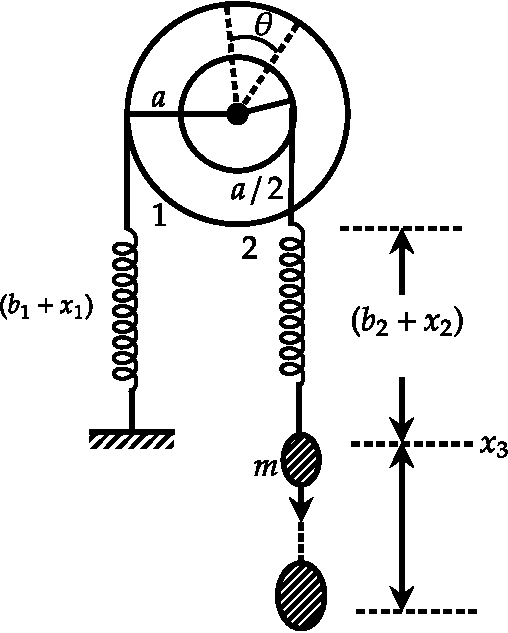
\includegraphics[height=6cm,width=5cm]{Lagrangian 03}
	\end{figure}
	Let $b_{1}$ and $b_{2}$ be the original length of the spring 1 and 2 . Which the whole system is in eq. and the DISC is stationary.\\
	Let $\theta$ be the angle the DISC has twined away from the eq. position. Then extension of the spring $-1$ is
	\begin{align*}
	x_{1}&=a \theta
	\intertext{If the spring $-2$ is stretched by a distance $x_{2}$ the mass $m$ is low ered by a distance}
	x_{3}&=\frac{a}{2} \theta+x_{2}\\
	K.E.\hspace{2cm}
	\mathrm{T}&=\mathrm{K} \cdot \mathrm{E} \cdot\text{ of }\mathrm{DISC}+\mathrm{K} \cdot \mathrm{E} \cdot\text{ of mass}\\
	&=\frac{1}{2}(\dot{\theta})^{2}+\frac{1}{2} m \dot{x}_{3}^{2}=\frac{1}{2} m a^{2} \cdot \dot{\theta}^{2}+\frac{1}{2} m\left(\frac{a}{2} \dot{\theta}+\dot{x}_{2}\right)^{2}\\
	P.E.
	\hspace{2cm}V&=\frac{1}{2} k x_{1}{ }^{2}+\frac{1}{2} k x_{2}{ }^{2}-m g x_{3} .
\intertext{	Hence the Lagrangian for the system is}
\mathrm{L}&=\mathrm{T}-\mathrm{V} \\
\mathrm{L}&=\frac{1}{2} m a^{2} \dot{\theta}^{2}+\frac{1}{2} m\left(\frac{a^{2}}{4} \dot{\theta}^{2}+a \dot{\theta} \dot{x}_{2}+\dot{x}_{2}^{2}\right)-\frac{1}{2} k x_{1}^{2}-\frac{1}{2} k x_{2}^{2}+m g\left(\frac{a}{2} \theta+x_{2}\right)\\
\text{Lagrangian eq. of motion, }&\frac{d}{d t}\left(\frac{\partial L}{\partial \dot{x}_{2}}\right)-\left(\frac{\partial L}{\partial x_{2}}\right)=0 \Rightarrow \frac{d}{d t}\left(\frac{\partial L}{\partial \dot{\theta}}\right)-\left(\frac{\partial L}{\partial \theta}\right)\\
\text { Or } \quad \frac{d}{d t}\left[\frac{1}{2} m a \theta+m \dot{x}_{2}\right]&-\left[-k x_{2}+m g\right]=0  \Rightarrow m \ddot{x}_{2}+k x_{2}+\frac{1}{2} m(a \ddot{\theta}-2 g)=0 \\ 
\text { Or } \quad \ddot{x}+\left(\frac{k}{m}\right) x_{2}&+\frac{1}{2}(a \ddot{\theta}-2 g)=0 \quad  \Rightarrow \frac{d}{d t}\left[\frac{1}{2} m a^{2} \dot{\theta}+\frac{1}{2} m a^{2}+\dot{\theta} \max _{2}\right]-\left[-k a^{2} \theta+\frac{m g a}{2}\right]\\
\text{Or }\quad \frac{3}{4} m a^{2} \ddot{\theta}&+R a^{2} \theta+\frac{1}{2} m a\left(\ddot{x}_{2}-g\right)=0\\
\text{Or }\quad \ddot{\theta}&+\left(\frac{4}{3} \frac{k}{m}\right) \theta+\frac{2}{3 a}\left(\ddot{x}_{2}-g\right)=0
\intertext{Which are the required equation of motion.}
	\end{align*}
\end{answer}
\item Set up the lagrangian for the following system, where the pully is massless.
\begin{figure}[H]
	\centering
	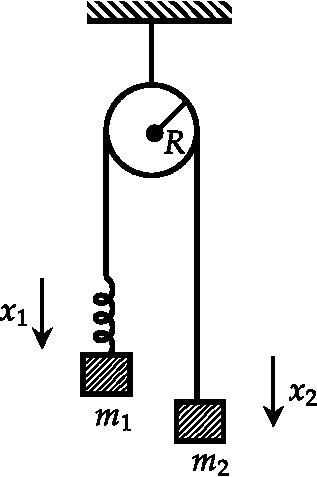
\includegraphics[height=6cm,width=4cm]{Lagrangian 04}
\end{figure}
\begin{answer}
	\begin{align*}
	\mathrm{T}&=\frac{1}{2} m_{1} \dot{x}_{1}^{2}+\frac{1}{2} m_{2} \dot{x}_{2}^{2}\\
	\mathrm{~V}&=-m_{1} g x_{1}-m_{2} g x_{2}+\frac{1}{2} k x_{1}^{2}\\
	\mathrm{~L}&=\frac{1}{2} m_{1} \dot{x}_{1}^{2}+\frac{1}{2} m_{2} \dot{x}_{2}^{2}+m_{1} g x_{1}+m_{2} g x_{2}-\frac{1}{2} k x_{1}^{2}\\
	\text{Thus, equation of motion is }&=\frac{d}{d t}\left(\frac{\partial L}{\partial \dot{x}_{1}}\right)-\left(\frac{\partial L}{\partial x_{1}}\right)=0\\
	\text{And }\frac{d}{d t}\left(\frac{\partial L}{\partial \dot{x}_{2}}\right)-\left(\frac{\partial L}{\partial x_{2}}\right)=0\\
	\Rightarrow \quad m_{1} \ddot{x}_{1}-m_{1} g+k x_{1}=0\\
	\text{Say, }m_{2} \ddot{x}_{2}-m_{2} g=0
	\end{align*}
\end{answer}
\item Set up the lagrangian for the following system, the disk also have mass ' $m$ '.
\begin{figure}[H]
	\centering
	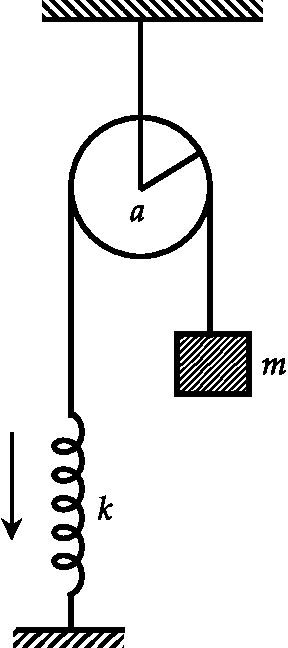
\includegraphics[height=6cm,width=2.7cm]{Lagrangian 11}
\end{figure}
\begin{answer}$\left. \right. $
	\begin{figure}[H]
		\centering
		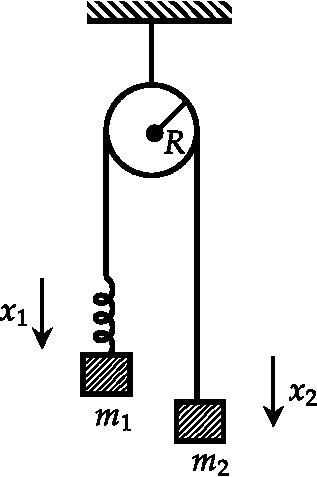
\includegraphics[height=6cm,width=4cm]{Lagrangian 04}
	\end{figure}
		Let $\theta$ be the angle one disc has turned away from one equilibrium position. Then extension of the spring $x_{1}=a \theta$\\
	Mass $m$ is lowered by a distance $x_{2}=\mathrm{a} \theta$
	\begin{align*}
\therefore \quad \mathrm{T} &=\frac{1}{2} m(a \dot{\theta})^{2}+\frac{1}{2} \mathrm{I} \dot{\theta}^{2} \\ \mathrm{~V} &=-\mathrm{mga} \theta+\frac{1}{2} k \theta^{2} a^{2} \\ \mathrm{~L} &=\frac{1}{2} m a^{2} \dot{\theta}^{2}+\frac{1}{4} m a^{2} \dot{\theta}^{2}+m g a \theta-\frac{1}{2} k a^{2} \theta^{2} \\
\text{Eq. of motion is}&
\frac{d}{d t}\left(\frac{\partial L}{\partial \theta}\right)-\frac{\partial L}{\partial \theta}=0\\
\Rightarrow \quad &m a^{2} \ddot{\theta}+\frac{1}{2} m a^{2} \ddot{\theta}-m g a+k a^{2} \theta=0\\
\Rightarrow \quad &\frac{3}{2} m a \ddot{\theta}-m g+k a \theta=0\\
\Rightarrow \quad &\ddot{\theta}-\frac{2}{3} g / a+\frac{2}{3}\left(\frac{k}{m}\right) \theta=0
	\end{align*}
\end{answer}
\item Two blocks connected by a spring of spring constant $k$ are free to slide frictionlessly along a horizontal surface, as shown in figure. The unstretched length of the spring is $a$.
\begin{figure}[H]
	\centering
	
\includegraphics[height=1cm,width=6cm]{Lagrangian 06}
\end{figure}
Two masses connected by a spring sliding horizontally along a frictionless surface.\\
(a) Identify a set of generalized coordinates and write the Lagrangian.
\begin{answer}
	As generalized coordinates I choose $X$ and $u$, where $X$ is the position of the right edge of the block of mass $M$, and $X+u+a$ is the position of the left edge of the block of mass $m$, where $a$ is the unstretched length of the spring. Thus, the extension of the spring is $u$. The Lagrangian is then
	\begin{align*}
	L&=\frac{1}{2} M \dot{X}^{2}+\frac{1}{2} m(\dot{X}+\dot{u})^{2}-\frac{1}{2} k u^{2}=\frac{1}{2}(M+m) \dot{X}^{2}+\frac{1}{2} m \dot{u}^{2}+m \dot{X} \dot{u}-\frac{1}{2} k u^{2}\\
	&\text{(b) Find the equation of motion.}\\
	&\text{The canonical momenta are}\\
	p_{X} &\equiv \frac{\partial L}{\partial \dot{X}}=(M+m) \dot{X}+m \dot{u}, p_{u} \equiv \frac{\partial L}{\partial \dot{u}}=m(\dot{X}+\dot{u})\\
	&\text{The corresponding equations of motion are then}\\
	&\dot{p}_{X}=F_{X}=\frac{\partial L}{\partial X} \quad \Rightarrow \quad(M+m) \ddot{X}+m \ddot{u}=0 \\
	&\dot{p}_{u}=F_{u}=\frac{\partial L}{\partial u} \quad \Rightarrow \quad m(\ddot{X}+\ddot{u})=-k u .
	\end{align*}
	(c) Find all conserved quantities.\\
	There are two conserved quantities. One is $p_{X}$ itself, as is evident from the fact that $L$ is cyclic in $X$. This is the conserved 'charge' $\Lambda$ associated with the continuous symmetry $X \rightarrow X+\zeta$. i.e. $\Lambda=p_{X}$. The other conserved quantity is the Hamiltonian $H$, since $L$ is cyclic in $t$. Furthermore, because the kinetic energy is homogeneous of degree two in the generalized velocities, we have that $H=E$, with
	\begin{align*}
	E&=T+U=\frac{1}{2}(M+m) \dot{X}^{2}+\frac{1}{2} m \dot{u}^{2}+m \dot{X} \dot{u}+\frac{1}{2} k u^{2} .\\
	\intertext{It is possible to eliminate $\dot{X}$, using the conservation of $\Lambda$ :}
	\dot{X}&=\frac{\Lambda-m \dot{u}}{M+m} .
	\intertext{This allows us to write}
	E&=\frac{\Lambda^{2}}{2(M+m)}+\frac{M m \dot{u}^{2}}{2(M+m)}+\frac{1}{2} k u^{2}
	\end{align*}
	(d) Find a complete solution to the equations of motion. As there are two degrees of freedom, your solution should involve 4 constants integration. You need not match initial conditions and you need not choose the quantities in part (c) to be among the constants.\\
	Using conservation of $\Lambda$, we may write $\ddot{X}$ in terms of $\ddot{x}$, in which case
	\begin{align*}
	\frac{M m}{M+m} \ddot{u}&=-k u \Rightarrow u(t)=A \cos (\Omega t)+B \sin (\Omega t)\\
\text{}\Omega&=\sqrt{\frac{(M+m) k}{M m}} .
\intertext{	For the $X$ motion, we integrate equation above, obtaining}
X(t)&=X_{0}+\frac{\Lambda t}{M+m}-\frac{m}{M+m}(A \cos (\Omega t)-A+B \sin (\Omega t))
\intertext{There are thus four constant: $X_{0}, \Lambda, A$ and $B$. Note that conservation of energy says}
E&=\frac{\Lambda^{2}}{2(M+m)}+\frac{1}{2} k\left(A^{2}+B^{2}\right)
	\end{align*}
	\textbf{Alternate solution :} We could choose $X$ as the position of the left block and $x$ as the position of the right block. In this case,
	\begin{align*}
	L&=\frac{1}{2} M \dot{X}^{2}+\frac{1}{2} m \dot{x}^{2}-\frac{1}{2} k(x-X-b)^{2} .
\intertext{	Here, $b$ includes the unstretched length $a$ of the spring, but may also include the size of the blocks if say, $X$ and $x$ are measured relative to the blocks midpoint. The canonical momenta are}
p_{X}&=\frac{\partial L}{\partial \dot{X}}=M \dot{X}, \quad p_{x}=\frac{\partial L}{\partial \dot{x}}=m \dot{x}
\intertext{The equation of motion are then}
\dot{p}_{X}&=F_{X}=\frac{\partial L}{\partial X} \quad \Rightarrow \quad M \ddot{X}=k(x-X-b) \\
\dot{p}_{x}&=F_{x}=\frac{\partial L}{\partial x} \quad \Rightarrow \quad m \ddot{x}=-k(x-X-b) .
\intertext{The one parameter family which leaves $L$ invariant is $X \rightarrow X+\zeta$ and $x \rightarrow x+\zeta$, i.e. simultaneous and identical displacement of both of the generalized coordinates. Then}
\Lambda&=M \dot{X}+m \dot{x}
\intertext{which is simply the $x$-components of the total momentum. Again, the energy is conserved.}
E&=\frac{1}{2} M \dot{X}^{2}+\frac{1}{2} m \dot{x}^{2}+\frac{1}{2} k(x-X-b)^{2} .
\intertext{We can combine the equations of motion to yield}
M m \frac{d^{2}}{d t^{2}}(x-X-b)&=-k(M+m)(x-X-b),
\intertext{which yields}
x(t)-X(t)&=b+A \cos (\Omega t)+B \sin (\Omega t)
\intertext{From the conservation of $\Lambda$, we have}
M X(t)+m x(t)&=\Lambda t+C
\intertext{where $C$ is another constant. Thus, we have the motion of the system in terms of four constant: $A, B, \Lambda$ and $C$ }
X(t)&=-\frac{m}{M+m}(b+A \cos (\Omega t)+B \sin (\Omega t))+\frac{\Lambda t+C}{M+m}\\
x(t)&=-\frac{M}{M+m}(b+A \cos (\Omega t)+B \sin (\Omega t))+\frac{\Lambda t+C}{M+m}
	\end{align*}
\end{answer}
\item A particle of charge $e$ moves in three dimensions in the presence of a uniform magnetic field $B=B_{0} \hat{z}$ and a uniform electric field $E=E_{0} \hat{x}$. The potential energy is
$$
U(r, \dot{r})=-e E_{0} x-\frac{e}{c} B_{0} x \dot{y},
$$
where we have chosen the gauge $A=B_{0} x \hat{y}$.\\
(a) Find the canonical momenta $p_{x}, p_{y}$ and $p_{z}$\\
(b) Identify all conserved quantities\\
(c) Find a complete, general solution for the motion of the system $\{x(t), y(t), x(t)\}$.
\begin{answer}
	\begin{align*}
	\text{( The Lagrangian is )}L&=\frac{1}{2} m\left(\dot{x}^{2}+\dot{y}^{2}+\dot{z}^{2}\right)+\frac{e}{c} B_{0} x \dot{y}+e E_{0} x. 
	\intertext{The canonical momenta are}
	p_{x}=\frac{\partial L}{\partial \dot{x}}&=m \dot{x} ; \quad p_{y}=\frac{\partial L}{\partial \dot{y}}=m \dot{y}+\frac{e}{c} B_{0} x ; \quad p_{x}=\frac{\partial L}{\partial \dot{z}}=m \dot{z}
\intertext{	(b) There are three conserved quantities. First is the momentum $p_{y}$, since $F_{y}=\frac{\partial L}{\partial y}=0 .$ Second is the momentum $p_{z}$, since $F_{y}=\frac{\partial L}{\partial z}=0$. The third conserved quantity is the Hamiltonian, since $\frac{\partial L}{\partial t}=0$. We have }
H&=p_{x} \dot{x}+p_{y} \dot{y}+p_{z} \dot{z}-L\\
\Rightarrow \quad H&=\frac{1}{2} m\left(\dot{x}^{2}+\dot{y}^{2}+\dot{z}^{2}\right)-e E_{0} x\\
\text{(c) The equations of motion are }\ddot{x}-\omega_{c} \dot{y}&=\frac{e}{m} E_{0} ; \ddot{y}+\omega_{c} \dot{x}=0 ; \ddot{z}=0.
\intertext{The second equation can be integrated once to yield $\dot{y}=\omega_{c}\left(x_{0}-x\right)$, where $x_{0}$ is a constant. Substituting this into the first equation gives}
\ddot{x}+\omega_{c}^{2} x&=\omega_{c}^{2} x_{0}+\frac{e}{m} E_{0} .
\intertext{This is the equation of a constantly forced harmonic oscillator. We can therefore write the generalsolution as}
x(t)&=x_{0}+\frac{e E_{0}}{m \omega_{c}^{2}}+A \cos \left(\omega_{c} t+\delta\right) \\
y(t)&=y_{0}-\frac{e E_{0}}{m \omega_{c}} t-A \sin \left(\omega_{c} t+\delta\right) \\
z(t)&=z_{0}+\dot{z}_{0} t
\intertext{Note that there are six constants, $\left\{A, \delta, x_{0}, y_{0}, z_{0}, \dot{z}_{0}\right\}$, are required for the general solution of three coupled second order ODEs.}
	\end{align*}
\end{answer}
\item A point mass $m$ slides frictionlessly, under the influence of gravity, along a massive ring of radius $a$ and mass $M$. The ring is affixed by horizontal springs to two fixed vertical surfaces, as depicted in figure. Allmotion is within the plane of the figure.
\begin{figure}[H]
	\centering
	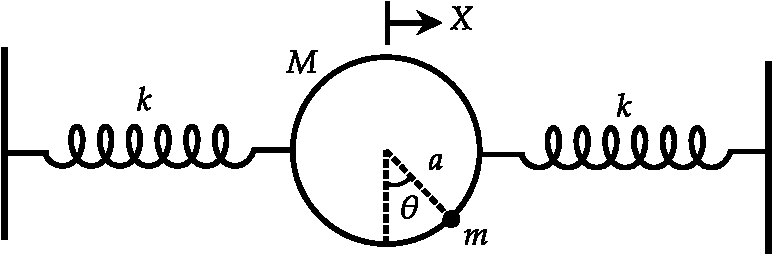
\includegraphics[height=2cm,width=6cm]{Lagrangian 07}
\end{figure}
A point mass $m$ slides frictionlessly along a massive ring of radius $a$ and mass $M$, which is affixed by horizontal springs to two fixed vertical surfaces.
\begin{answer}
	(a) Choose as generalized coordinates the horizontal displacement $X$ of the center of the ring with respect to equilibrium, and the angle $\theta$ a radius to the mass $m$ makes with respect to the vertical (see figure). You may assume that at $X=0$ the spring are both unstretched. Find the Lagrangian $L(X, \theta, \dot{X}, \dot{\theta}, t)$.\\
	The coordinates of the mass point are $x=X+a \sin \theta, y=-a \cos \theta$.\\
	The kinetic energy is
	\begin{align*}
T &=\frac{1}{2} M \dot{X}^{2}+\frac{1}{2} m(\dot{X}+a \cos \theta \dot{\theta})^{2}+\frac{1}{2} m a^{2} \sin ^{2} \theta \dot{\theta}^{2} \\ &=\frac{1}{2}(M+m) \dot{X}^{2}+\frac{1}{2} m a^{2} \dot{\theta}^{2}+m a \cos \theta \dot{X} \dot{\theta} .\\
\text{The potential energy is }U&=k X^{2}-m g a \cos \theta.\\
\text{Thus, the Lagrangian is}&=\frac{1}{2}(M+m) \dot{X}^{2}+\frac{1}{2} m a^{2} \dot{\theta}^{2}+m a \cos \theta \dot{X}-k X^{2}+m g a \cos \theta.
\intertext{(b) Find the generalized momenta $p_{X}$ and $p_{\theta}$, and the generalized forces $F_{X}$ and $F_{\theta}$}
\text{We have }p_{X}&=\frac{\partial L}{\partial \dot{X}}=(M+m) \dot{X}+m a \cos \theta \dot{\theta}, p_{\theta}=\frac{\partial L}{\partial \dot{\theta}}=m a^{2} \dot{\theta}+m a \cos \theta \dot{X}.\\
\text{For the forces, }F_{X}&=\frac{\partial L}{\partial X}=-2 k X, \quad F_{\theta}=\frac{\partial L}{\partial \theta}=-m a \sin \theta \dot{X} \dot{\theta}-m g a \sin \theta.
\intertext{(c) Derive the equations o motion.}
\text{The equations of motion arc }&\frac{d}{d t}\left(\frac{\partial L}{\partial \dot{q}_{\sigma}}\right)=\frac{\partial L}{\partial q_{\sigma}}, \text{for each generalized coordinate }q_{\sigma} .\text{ For $X$ we have }\\
(M+m) \ddot{X}+m a \cos \theta \ddot{\theta}-m a \sin \theta \dot{\theta}^{2}&=-2 k X .\\
\text{For }\theta, m a^{2} \ddot{\theta}+m a \cos \theta \ddot{X}&=-m g a \sin \theta.
\intertext{(d) Find expression for all conserved $_{1}$ uantities.}
\intertext{Horizontal and vertical translationa $^{1}$ symmetries are broken by the springs and by gravity, respectively. The remaining symmetry is that of time translation. From $\frac{d H}{d t}=-\frac{\partial L}{\partial t}$, we have that $H=\sum_{\sigma} p_{\sigma} \dot{q}_{\sigma}-L$ is conserved. For this problem, the kinetic energy is a homogeneous function of degree 2 in the generalized velocities, and the potential is velocity-independent. Thus,}
H=T+U&=\frac{1}{2}(M+m) \dot{X}^{2}+\frac{1}{2} m a^{2} \dot{\theta}^{2}+m a \cos \theta \dot{X} \dot{\theta}+k X^{2}-m g a \cos \theta
	\end{align*}
\end{answer}
\item A point particle of mass $m$ moves in three dimensions in a helical potential
$$
U(\rho, \phi, z)=U_{0} \rho \cos \left(\phi-\frac{2 \pi z}{b}\right)
$$
We call $b$ the pitch of the helix.
\begin{answer}
	\begin{align*}
	\intertext{(a) Write down the Lagrangian, choosing $(\rho, \phi, z)$ as generalized coordinates.}
\text{	The Lagrangian is }L&=\frac{1}{2} m\left(\dot{\rho}^{2}+\rho^{2} \dot{\phi}^{2}+\dot{z}^{2}\right)-U_{0} \rho \cos \left(\phi-\frac{2 \pi z}{b}\right)
\intertext{	(b) Find the equation of motion.}
	\text{Clearly }p_{\rho}&=m \dot{\rho} ; p_{\phi}=m \rho^{2} \dot{\phi} ; p_{z}=m \dot{z},\text{ and}\\
	F_{\rho}=m \rho \dot{\phi}^{2}-U_{0} \cos \left(\phi-\frac{2 \pi z}{b}\right), F_{\phi}&=U_{0} \rho \sin \left(\phi-\frac{2 \pi z}{b}\right), F_{z}=-\frac{2 \pi U_{0}}{b} \rho \sin \left(\phi-\frac{2 \pi z}{b}\right) \text {. }
\intertext{	Thus, the equation of motion are}
	m \ddot{\rho}&=m \rho \dot{\phi}^{2}-U_{0} \cos \left(\phi-\frac{2 \pi z}{b}\right) \\
	m \rho^{2} \ddot{\phi}+2 m \rho \dot{\rho} \dot{\phi}&=U_{0} \rho \sin \left(\phi-\frac{2 \pi z}{b}\right)\\
	m \ddot{z}&=-\frac{2 \pi U_{0}}{b} \rho \sin \left(\phi-\frac{2 \pi z}{b}\right)
	\intertext{(c) Show that there exists a continuous one-parameter family of coordinate transformations which leaves $L$ invariant. Find the associated conserved quantity, $\Lambda$. Is anything else conserved?}
	\intertext{Due to the helical symmetry, we have that $\phi \rightarrow \phi+\zeta, z \rightarrow z+\frac{b}{2 \pi} \zeta$ is such a continuous one-parameter}
	\intertext{family of coordinate transformations. Since it leaves the combination $\phi-\frac{2 \pi z}{\dot{b}}$ unchanged, we have that $\frac{d L}{d \zeta}=0$, and}
\Lambda &=\left.p_{\rho} \frac{\partial \rho}{\partial \zeta}\right|_{\zeta=0}+\left.p_{\phi} \frac{\partial \phi}{\partial \zeta}\right|_{\zeta=0}+\left.p_{z} \frac{\partial z}{\partial \zeta}\right|_{\zeta=0} \\ &=p_{\phi}+\frac{b}{2 \pi} p_{z} \\ &=m \rho^{2} \dot{\phi}+\frac{m b}{2 \pi} \dot{z}
\intertext{is the conserved Noether 'charge'. The other conserved quantity is the Hamiltonian,}
H&=\frac{1}{2} m\left(\dot{\rho}^{2}+\rho^{2} \dot{\phi}^{2}+\dot{z}^{2}\right)+U_{0} \rho \cos \left(\phi-\frac{2 \pi z}{b}\right)
\intertext{Note that $H=T+U$ because $T$ is homogeneous of degree 2 and $U$ is homogeneous of degree 0 in the generalized velocities.} 
	\end{align*}
\end{answer}
\textbf{Statement for Linked Answer Q.12 and Q.13 :}\\
A particle of mass $m$ is constrained to move in a vertical plane along a trajectory given by $x=\mathrm{A} \cos \theta$, $y=\mathrm{A} \sin \theta$, where $\mathrm{A}$ is a constant.
\item The Lagrangian of the particle is
 \begin{tasks}(2)
	\task[\textbf{a.}]$\frac{1}{2} m \mathrm{~A}^{2} \dot{\theta}^{2}-m g \mathrm{~A} \cos \theta$
	\task[\textbf{b.}]$\frac{1}{2} m \mathrm{~A}^{2} \dot{\theta}^{2}-m g \mathrm{~A} \sin \theta$
	\task[\textbf{c.}] $\frac{1}{2} m \mathrm{~A}^{2} \dot{\theta}^{2}$
	\task[\textbf{d.}] $\frac{1}{2} m \mathrm{~A}^{2} \dot{\theta}^{2}+m g \mathrm{~A} \cos \theta$
\end{tasks}
\begin{answer}$\left. \right. $
	\begin{figure}[H]
		\centering
		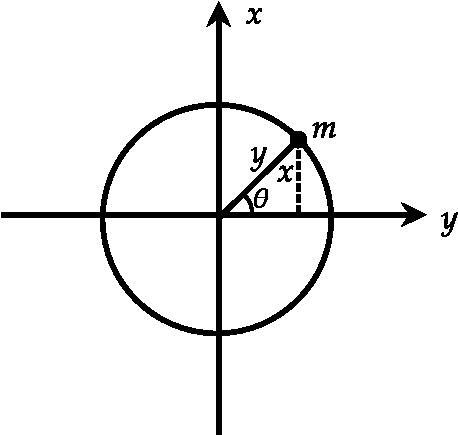
\includegraphics[height=4.2cm,width=4.5cm]{Lagrangian 08}
	\end{figure}
	\begin{align*}
	L&=T-V\\
	L&=\frac{1}{2} m\left(\dot{x}^{2}+\dot{y}^{2}\right)-m g y^{x}\\
	x&=A \cos \theta, \quad y=A \sin \theta\\
	\dot{x}&=-A \sin \theta \dot{\theta}, \quad \dot{y}=A \cos \theta \dot{\theta}\\
	 \therefore \quad L &=\frac{1}{2} m\left(A^{2} \sin ^{2} \theta \dot{\theta}^{2}+A^{2} \cos ^{2} \theta \dot{\theta}^{2}\right)-m g A \cos \theta \\ L &=\frac{1}{2} m A^{2} \dot{\theta}^{2}-m g A \cos \theta 
	\end{align*}
	 Correct answer is option \textbf{(a)}
\end{answer}
\item The equation of motion of the particle is
 \begin{tasks}(2)
	\task[\textbf{a.}]$\ddot{\theta}-\frac{g}{\mathrm{~A}} \cos \theta=0$
	\task[\textbf{b.}]$\ddot{\theta}+\frac{g}{\mathrm{~A}} \sin \theta=0$
	\task[\textbf{c.}] $\ddot{\theta}=0$
	\task[\textbf{d.}]  $\ddot{\theta}-\frac{g}{\mathrm{~A}} \sin \theta=0$
\end{tasks}
\begin{answer}
	Equation of motion
	\begin{align*}
	\frac{d}{d t}\left(\frac{\partial L}{\partial \dot{\theta}}\right)-\frac{\partial L}{\partial \theta}&=0\\
	\frac{d}{d t}\left(m A^{2} \dot{\theta}\right)-m g A \sin \theta&=0\\
	m A^{2} \ddot{\theta}-m g A \sin \theta&=0\\
	\ddot{\theta}-\frac{g}{A} \sin \theta&=0
	\end{align*}
	Correct answer is option \textbf{(d)}
\end{answer}
\item A particle of mass $M$ is attached to two identical springs of unstretched length $L_{0}$ and spring constant $k$. The entire system is placed on a horizontal frictionless table as shown in the figure. The mass is slightly puled along the surface of the table and perpendicular to the lengths of the springs and then let go. Using the Lagrangian equation (s) of motion, show whether the mass will execute simple harmonic motion. If so, find the time period.
\begin{figure}[H]
	\centering
	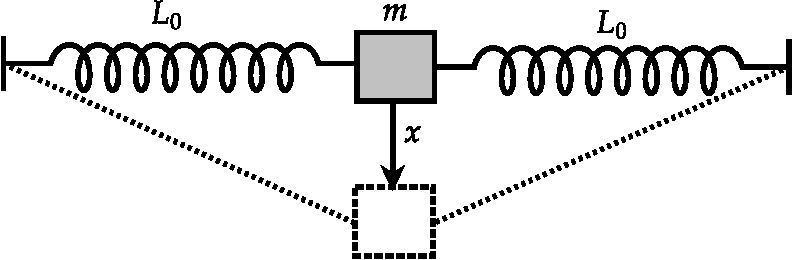
\includegraphics[height=2.5cm,width=7cm]{Lagrangian 09}
\end{figure}
\begin{answer}$\left. \right. $
	\begin{figure}[H]
		\centering
		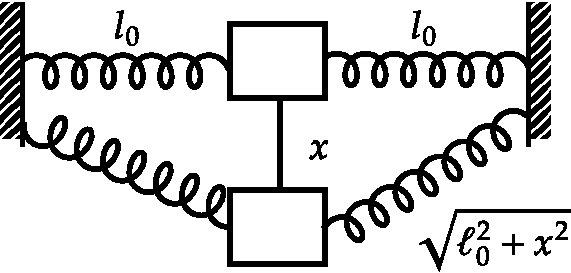
\includegraphics[height=2.5cm,width=6cm]{Lagrangian 10}
	\end{figure}
	\begin{align*}
\text{	Kinetic energy }T&=\frac{1}{2} m \dot{x}^{2}\\
\text{	potential energy }V&=\frac{1}{2} k\left(\sqrt{\ell_{0}^{2}+x^{2}}-\ell_{0}\right)^{2}
\intertext{Number gravitational potential energy term because motion is taking place in horizontal plane.}
\text{Lagrangian }L&=T-V=\frac{1}{2} m \dot{x}^{2}-\frac{1}{2} k\left(\sqrt{\ell_{0}^{2}+x^{2}}-\ell_{0}\right)^{2}
\intertext{Lagrange's equation}
&\frac{d}{d t}\left(\frac{\partial L}{\partial \dot{x}}\right)-\frac{\partial L}{\partial x}=0 \\
&m \ddot{x}+2 k\left(\sqrt{\ell_{0}^{2}+x^{2}}-\ell_{0}\right) \frac{x}{\sqrt{\ell_{0}^{2}+x^{2}}}=0 \\
&m \ddot{x}+2 k x\left(1-\frac{\ell_{0}}{\sqrt{\ell_{0}^{2}+x^{2}}}\right)=0\\
\text{for }&x<<\ell_{0} \quad m \ddot{x}+2 k x\left(1-\left(1+\frac{x^{2}}{\ell_{0}^{2}}\right)^{-1 / 2}\right)=0\\
m \ddot{x}+2 k x\left(1-1+\frac{x^{2}}{2 \ell_{0}^{2}}\right)&=0 \Rightarrow m \ddot{x}+\frac{k x^{3}}{\ell_{0}^{2}}=0 \ddot{x} \alpha-x^{3}
\intertext{Motion is not simple harmonic.}
	\end{align*}
\end{answer}
\end{enumerate}
\section{Hamiltonian Mechanics}
\begin{enumerate}
	\item Show that $\frac{d H}{d t}=\frac{\partial H}{\partial t}$
	\begin{answer}
		\begin{align*}
		\text{Since }H&=H\left(q_{j}, p_{j}, t\right)\\
		\therefore \quad \frac{d H}{d t} & =\frac{\partial H}{\partial t}+\sum_{j} \frac{\partial H}{\partial q_{j}}+\sum_{j} \frac{\partial H}{\partial p_{j}} \dot{p}_{j} \Rightarrow \frac{d H}{d t}=\frac{\partial H}{\partial t}+\sum_{j}\left(-\dot{p}_{j} \dot{q}_{j}\right)+\sum_{k}\left(\dot{q}_{j} \dot{p}_{j}\right) \\
		\therefore \quad \frac{d H}{d t} & =\frac{\partial H}{\partial t}
		\end{align*}
	\end{answer}
	\item Obtain the Hamiltonian function of a compound pendulum and hence obtain the equation describing its motion.
	\begin{answer}
		The pendulum is a harmonic conservative system. It is holonomic because the constraint is on the position of the pendulum in the sense that it must vibrate in its own plane and conservative because the gravitational force acting on it is conservative. With reference to a frame fixed at the point of suspension with downward vertical as the reference line, we have
		\begin{align*}
		T&=\frac{1}{2} I \dot{\theta}^{2}
	\intertext{	where $I$ is the moment of inertia of the pendulum about the axis passing through the point suspension and perpendicular to its plane.}
		V&=-m g \ell \cos \theta
	\intertext{	where $\ell$ is the distance of the centre of gravity from the centre of suspension.}
\therefore & H=T+V=\frac{1}{2} I \dot{\theta}^{2}-m g \ell \cos \theta \\ \text { Now, } & p_{\theta}=\frac{\partial T}{\partial \dot{\theta}}=I \dot{\theta} \\ \therefore & H=\frac{1}{2} I \frac{p_{\theta}^{2}}{I^{2}}-m g \ell \cos \theta \\ \text { Or, } & H=\frac{p_{\theta}^{2}}{I^{2}}-m g \ell \cos \theta \\ & \frac{\partial H}{\partial p_{\theta}}=\frac{p_{\theta}}{I} \text { and } \frac{\partial H}{\partial p_{\theta}}=-m g \ell(-\sin \theta)=m g \ell \sin \theta\\
\text{By Hamilton's general equations }&\left(\dot{p}_{k}=-\frac{\partial H}{\partial q_{k}}\right.\text{ and }
\left.\dot{q}_{k}=\frac{\partial H}{\partial p_{k}}\right)\\
\text{We have here }\dot{p}_{\theta}&=-\frac{\partial H}{\partial \theta}=-m g \ell \sin \theta\text{ and }\dot{\theta}=\frac{\partial H}{\partial p_{\theta}}=\frac{p_{\theta}}{I}
\intertext{These are the two equations describing the motion of a compound pendulum. However, these two equaions can be combined into a signle equation. Differentiating the second equation and eliminating $\dot{p}_{\theta}$,}
\intertext{we have}
\ddot{\theta}&=\frac{\dot{p}_{\theta}}{I} \sin \theta ; \text { or } \ddot{\theta}+\frac{m g I}{I} \sin \theta=0
\intertext{This is the required single equation that describes the motion of a compound pendulum.}
		\end{align*}
	\end{answer}
	\item A particle moves in the $x y$ plane under the influence of a central force depending on its distance from the origin.\\
	(a) Set up the Hamiltonian for the system\\
	(b) Obtain Hamilton's equations of motion
	\begin{answer}
	\begin{align}
	\text{(a) }T \text{(kinetic energy of of the particle) }&=\frac{1}{2 m \dot{r}^{2}}+\frac{1}{2} I \dot{\theta}^{2}=\frac{1}{2} m \dot{r}^{2}+\frac{1}{2} m r^{2} \dot{\theta}^{2}\quad
	\left(\because I=m r^{2}\right)\notag\\
\therefore & H=T+V=\frac{1}{2} m \dot{r}^{2}+\frac{1}{2} m r^{2} \dot{\theta}^{2}+V(r)\notag \\ \text { Now, } & p_{r}=\frac{\partial T}{\partial \dot{r}}=m \dot{r} \text { and } p_{\theta}=\frac{\partial T}{\partial \dot{\theta}}=I \dot{\theta}=m r^{2} \dot{\theta} \notag\\ \therefore & H=\frac{1}{2} m \cdot \frac{p_{r}^{2}}{m^{2}}+\frac{1}{2} m r^{2} \frac{p_{\theta}^{2}}{m^{2} r^{4}}+V(r) \notag\\ \text { Or, } & H=\frac{p_{r}^{2}}{2 m}+\frac{p_{\theta}^{2}}{2 m r^{2}}+V(r)\notag
\intertext{(b) We have from Hamilton's equation,}
&\left(\dot{p}_{k}=-\frac{\partial H}{\partial q_{k}} \text { and } \dot{q}_{k}=\frac{\partial H}{\partial p_{k}}\right) \notag\\
&\dot{p}_{r}=-\frac{\partial H}{\partial r}=-\left(-\frac{p_{\theta}^{2}}{m r^{3}}+\frac{\partial V}{\partial r}\right)=\frac{p_{\theta}^{2}}{m r^{3}}-\frac{\partial V}{\partial r} \label{HM-29}\\
&\dot{r}=\frac{\partial H}{\partial p_{r}}=\frac{p_{r}}{m} \label{HM-30}\\
&\dot{p}_{\theta}=-\frac{\partial H}{\partial \theta}=0 \label{HM-31}\\
&\dot{\theta}=\frac{\partial H}{\partial p_{\theta}}=\frac{p_{\theta}}{m r^{2}}\label{HM-32}
\intertext{Equations (\ref{HM-29}), (\ref{HM-30}), (\ref{HM-31}) and (\ref{HM-32}) are the required Hamilton's equations. However they can be combined to reduce the number of equations describing the motion. Equations (\ref{HM-29}) and (\ref{HM-30}) combine into (after elimination of $\dot{p}_{r}$ )}\notag
\ddot{r}&=\frac{p_{\theta}^{2}}{m^{2} r^{3}}-\frac{1}{m} \frac{\partial V}{\partial r}=\frac{m^{2} r^{4} \dot{\theta}^{2}}{m^{2} r^{2}}-\frac{1}{m} \frac{\partial V}{\partial r}\notag
\intertext{and (\ref{HM-31}) and (\ref{HM-32}) combine into (after elimination of $\dot{p}_{\theta}$ ) $\ddot{\theta}=0$ Thus the equations describing motion of the particle are}
\ddot{r}-r \dot{\theta}^{2}&=-\frac{1}{m} \frac{\partial V}{\partial r} \text { and } \ddot{\theta}=0\notag\\
\text{Or, }\quad \ddot{r}-r \dot{\theta}^{2}&=-\frac{1}{m} \frac{\partial V}{\partial r}\text{ and }\dot{\theta}=\frac{p_{\theta}}{m r^{2}}=\frac{a \text { constant }}{m r^{2}}\notag\\
\quad\left(\because p_{\theta}=a\right.&\text{ constant from }\left.(i i i)\right)\text{
	Or, }\quad m r^{2} \dot{\theta}=a\text{ constant}\notag
	\end{align}
	\end{answer}
	\item The Hamiltonian of a simple pendulum consisting of a mass ' $\mathrm{m}$ ' attached to a massless string of length $l$ is $\mathrm{H}=\frac{\mathrm{p}_{\theta}^{2}}{2 \mathrm{~m} \ell^{2}}+\mathrm{mg} \ell(1-\cos \theta)$. If L denotes the Lagrangian, the value of $\frac{\mathrm{dL}}{\mathrm{dt}}$ is :
	 \begin{tasks}(2)
		\task[\textbf{a.}]$-\frac{2 g}{\ell} p_{\theta} \sin \theta$
		\task[\textbf{b.}]$-\frac{\mathrm{g}}{\ell} \mathrm{p}_{\theta} \sin 2 \theta$
		\task[\textbf{c.}] $\frac{\mathrm{g}}{\ell} \mathrm{p}_{\theta} \cos \theta$
		\task[\textbf{d.}] $\ell \mathrm{p}_{\theta}^{2} \cos \theta$
	\end{tasks}
	\begin{answer}
		\begin{align*}
		\mathrm{H}&=\frac{\mathrm{p}_{\theta}^{2}}{2 \mathrm{~m} \ell^{2}}+\mathrm{mg} \ell(1-\cos \theta) \Rightarrow \mathrm{L}=\sum_{\mathrm{i}} \mathrm{p}_{\mathrm{i}} \dot{\mathrm{q}}_{\mathrm{i}}-\mathrm{H}=\mathrm{p}_{\theta} \dot{\theta}-\mathrm{H}\\
		\dot{\theta}&=\frac{\partial \mathrm{H}}{\partial \mathrm{p}_{\theta}}=\frac{\mathrm{p}_{\theta}}{\mathrm{m} \ell^{2}}\text{ and }\dot{\mathrm{p}}_{\theta}=-\frac{\partial \mathrm{H}}{\partial \theta}=-\mathrm{mg} \ell \sin \theta\\
		\text{Therefore, }\mathrm{L}&=\mathrm{p}_{\theta} \frac{\mathrm{p}_{\theta}}{\mathrm{m} \ell^{2}}-\left[\frac{\mathrm{p}_{\theta}^{2}}{2 \mathrm{~m} \ell^{2}}+\mathrm{mg} \ell(1-\cos \theta)\right] \Rightarrow \mathrm{L}=\frac{\mathrm{p}_{\theta}^{2}}{2 \mathrm{~m} \ell^{2}}-\mathrm{mg} \ell(1-\cos \theta)\\
		\text{Since, }L&=L\left(\theta, p_{\theta}\right)\text{Since, }
		 -\frac{L}{1}=\frac{\partial L}{\partial p_{\theta}} \dot{p}_{\theta}+\frac{\partial L}{\partial \theta} \dot{\theta}\\
		 \text{Now, }\frac{\partial \mathrm{L}}{\partial \mathrm{p}_{\theta}}&=\frac{\mathrm{p}_{\theta}}{\mathrm{m} \ell^{2}}, \quad \dot{\mathrm{p}}_{\theta}=-1.1 \mathrm{~g} \ell \sin \theta, \quad \frac{\partial \mathrm{L}}{\partial \theta}=-\mathrm{mg} \ell \sin \theta, \quad \dot{\theta}=\frac{\mathrm{p}_{\theta}}{\mathrm{m} \ell^{2}} \\
		 \text{Then} \frac{\mathrm{dL}}{\mathrm{dt}}&=\frac{\mathrm{p}_{\theta}}{\mathrm{m} \ell^{2}}(-\mathrm{mg} \ell \sin \theta)-\mathrm{mg} \ell \quad \mathrm{n} \theta \frac{\mathrm{p}_{\theta}}{\mathrm{m} \ell^{2}}=-\frac{2 \mathrm{~g}}{\ell} \mathrm{p}_{\theta} \sin \theta
		\end{align*}
		Correct option is \textbf{(a)}
	\end{answer}
	\item The particel of mass $m$ is constrained to move on the surface of a cylinder of radius $a$ under an attractive central force $F$, given by
	$$
	F=-k r
	$$
	where $k$ is the force constant. This force is proportional to the distance of the particle from the origin
\begin{answer}
		The motion of the particle can be described in terms of the cartesian coordinates $\mathrm{x}, \mathrm{y}, \mathrm{z}$ or cylindrical $\rho, \theta, z$ (See figure). The equation of constraint is
		\begin{figure}[H]
			\centering
			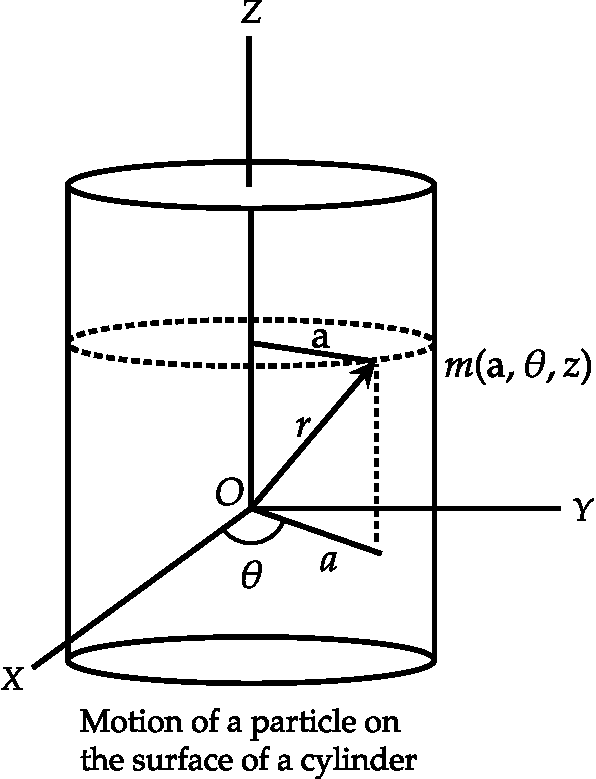
\includegraphics[height=7cm,width=4.5cm]{Lagrangian 12}
		\end{figure}
	\begin{align}
	\rho^{2}&=x^{2}+y^{2}=a^{2}\label{HM-33-}
\intertext{	To find velocity in cylinderical coordinates, we can proceed as follows}\notag
\text{The change in position along }\rho&=d \rho\notag\\
\text{The change in position along }\theta&=\rho d \theta\notag\\
\text{The change in position along }z&=d z
\text{So, }v_{\rho}=\dot{\rho}, v_{\theta}=\rho \dot{\theta}\text{and} v_{z}=\dot{z}\notag\\
\text{So, we have }v^{2}&=v_{\rho}^{2}+v_{\theta}^{2}+v_{z}^{2}.\notag\\
\text{The kinetic energy, }T&=\frac{1}{2} m v^{2}=\frac{1}{2}\left(\dot{\rho}^{2}+\rho^{2} \dot{\theta}^{2}+\dot{z}^{2}\right)\notag\\
\text{Here, }\rho&=a\notag\\
\text{Therefore, }\dot{\rho}&=0,\text{ and hence,}\notag\\
T &=\frac{1}{2} m\left(a^{2} \dot{\theta}^{2}+\dot{z}^{2}\right) \notag\\ \text{and}\quad V &=\frac{1}{2} k r^{2}=\frac{1}{2} k\left(x^{2}+y^{2}+z^{2}\right)=\frac{1}{2} k\left(a^{2}+z^{2}\right)\notag\\
\therefore \quad L=T-V&=\frac{1}{2} m\left(a^{2} \dot{\theta}^{2}+\dot{z}^{2}\right)-\frac{1}{2} k\left(a^{2}+z^{2}\right)\label{HM-34-}\\
\text{Hence,}
p_{\theta}&=\frac{\partial L}{\partial \dot{\theta}}=m a^{2} \dot{\theta}\text{ or} \dot{\theta}=\frac{p_{\theta}}{m a^{2}}\notag\\
\text{and }\quad p_{z}&=\frac{\partial L}{\partial \dot{z}}=m \dot{z}\text{ or} \dot{z}=\frac{p_{z}}{m}\notag\\
\text{Therefore, }\quad H&=T+V=\frac{1}{2} m\left(a^{2} \dot{\theta}+\dot{z}^{2}\right)+\frac{1}{2} k\left(a^{2}+z^{2}\right)\notag\\
\text { Or, } \quad H&=\frac{p_{\theta}^{2}}{2 m a^{2}}+\frac{p_{z}^{2}}{m}+\frac{1}{2} k\left(a^{2}+z^{2}\right)\label{HM-35-}
\intertext{Hence, the Hamilton's equation are}\notag\\
\dot{z}&=\frac{\partial H}{\partial p_{z}}=\frac{p_{z}}{m}\text{ or }p_{z}=m \dot{z}\label{HM-36-}\\
\dot{\theta}&=\frac{\partial H}{\partial p_{\theta}}=\frac{p_{\theta}}{m a^{2}}\text{ or }p_{\theta}=m a^{2} \dot{\theta}\label{HM-37-}\\
-\dot{p}_{z}&=\frac{\partial H}{\partial z}=k z \quad\text{ or }\quad \dot{\mathrm{p}}_{z}=-k z\label{HM-38-}\\
-\dot{p}_{\theta}&=\frac{\partial H}{\partial \theta}=0 \quad\text{ or }
p_{\theta}= \text{constant}\label{HM-39-}
\intertext{From equation (\ref{HM-36-}) and (\ref{HM-38-}), we get}
m \ddot{z}+k z&=0\notag
\intertext{which shows that the motion of the particle in z direction is simple harmonic with period $T$, given by}\notag
T&=2 \pi \sqrt{\frac{m}{k}}\notag
\intertext{From equation (\ref{HM-37-}) and (\ref{HM-39-}), we get}\notag
p_{\theta}&=m a^{2} \dot{\theta}=\text { constant }\notag
\intertext{Thus the angular momentum about Z-axis is a constant of motion.}\notag
	\end{align}
\end{answer}
	\item Find equations of motion of particle moving near the surface of earth.
	\begin{answer}
		\begin{align*}
		\intertext{Let us consider z-axis along upward vertical direction, the kinetic energy is}
		T&=\frac{1}{2} m\left(\dot{x}^{2}+\dot{y}^{2}+\dot{z}^{2}\right)
	\intertext{	Further the applied force on the body is its weight acting in negative z-direction, i.e.,}
		F&=F_{z}-m g=-\frac{\partial V}{\partial Z}
		\intertext{This gives $V=m g Z$, on setting additive constant to zero Now} 
	\intertext{	Lagrangian is}
		L&=T-V=\frac{1}{2} m\left(\dot{x}^{2}+\dot{y}^{2}+\dot{z}^{2}\right)-m g Z\\
		\text{So that }\frac{\partial L}{\partial \dot{x}}&=\frac{\partial T}{\partial \dot{x}}=p_{x}=m \dot{x}\text{ giving }\dot{x}=\frac{p_{x}}{m}\\
	\text{	Also, }p_{y}&=m \dot{y}, p_{z}=m \dot{z}\\
		\therefore \quad \dot{y}&=\frac{p_{y}}{m}, \dot{z}=\frac{p_{z}}{m}\\
	\intertext{	Hamiltonian for such a system is conserved, i.e.,}
		H&=T+V=\frac{1}{2}\left(\dot{x}^{2}+\dot{y}^{2}+\dot{z}^{2}\right)+m g Z=\frac{1}{2 m}\left(p_{x}^{2}+p_{y}^{2}+p_{z}^{2}\right)+m g Z \\
		\intertext { giving equations of motion }
		\dot{p}_{x}&=-\frac{\partial H}{\partial x}=0, \quad \dot{p}_{y}=-\frac{\partial H}{\partial y}=0\\
		\dot{p}_{z}&=-\frac{\partial H}{\partial Z}=-m g\\
		\therefore \quad \dot{x}&=\frac{\partial H}{\partial p_{x}}=\frac{p_{x}}{m}, \quad \dot{y}=\frac{\partial H}{\partial p_{y}}=\frac{p_{y}}{m}, \dot{z}=\frac{\partial H}{\partial Z}=\frac{p_{z}}{m}
	\intertext{ so we finally get,}
		\ddot{x}&=\frac{\dot{p}_{y}}{m}=0, \quad \ddot{y}=\frac{\dot{p}_{y}}{m}=0, \quad \ddot{z}=\frac{\dot{p}_{z}}{m}=-g
		\end{align*}
	\end{answer}
	\item A mechanical system is described by the Hamiltonian $H(q, p)=\frac{p^{2}}{2 m}+\frac{1}{2} m \omega^{2} q^{2}$. As a result of the canonical transformation generated by $F(q, Q)=-\frac{Q}{q}$, the Hamiltonian in the new coordinate $Q$ and momentum $P$ becomes
	 \begin{tasks}(2)
		\task[\textbf{a.}]$\frac{1}{2 m} Q^{2} P^{2}+\frac{m \omega^{2}}{2} Q^{2}$
		\task[\textbf{b.}]$\frac{1}{2 m} Q^{2} P^{2}+\frac{m \omega^{2}}{2} P^{2}$
		\task[\textbf{c.}]$\frac{1}{2 m} P^{2}+\frac{m \omega^{2}}{2} Q^{2}$
		\task[\textbf{d.}] $\frac{1}{2 m} Q^{2} P^{4}+\frac{m \omega^{2}}{2} P^{-2}$
	\end{tasks}
	\begin{answer}
		\begin{align*}
		F(q, Q)&=-\frac{Q}{q}
	\intertext{	Differential relation for $F(q, Q)$}
		p&=\frac{\partial F}{\partial q}, \quad P=-\frac{\partial F}{\partial Q}\\
		\text{So, }\quad p&=\frac{Q}{q^{2}}, P=\frac{1}{q} \quad \Rightarrow p=Q P^{2}
	\intertext{	New Hamiltonian,}
		H^{\prime}&=H+\frac{\partial F}{\partial t}=H+0\\
		H^{\prime}(Q, P)&=H(q, p)=\frac{p^{2}}{2 m}+\frac{1}{2} m \omega^{2} q^{2}=\frac{1}{2 m} Q^{2} P^{4}+\frac{1}{2} m \omega^{2} P^{-2}
		\end{align*}
		Correct answer is option \textbf{(d)}
	\end{answer}
\end{enumerate}
\section{Small Oscillations}
\begin{enumerate}
	\item  A particle of mass $m$ moves in one dimension under the influence of a potential energy
	$$
	V(x)=-a\left(\frac{x}{\ell}\right)^{2}+b\left(\frac{x}{\ell}\right)^{4}
	$$
	where $a$ and $b$ are positive constants and $\ell$ is a characteristic length. The frequency of small oscillations about a point of stable equilibrium is:
	 \begin{tasks}(2)
		\task[\textbf{a.}] $\frac{1}{2 \pi \ell} \sqrt{\frac{b}{m}}$
		\task[\textbf{b.}]$\frac{2 b}{\pi \ell} \sqrt{\frac{1}{m a}}$
		\task[\textbf{c.}]$\frac{1}{\pi \ell} \sqrt{\frac{a^{2}}{m b}}$
		\task[\textbf{d.}] $\frac{1}{\pi \ell} \sqrt{\frac{a}{m}}$
	\end{tasks}
	\begin{answer}
		\begin{align*}
	\text{	We have,}
		V(x)&=-a\left(\frac{x}{\ell}\right)^{2}+b\left(\frac{x}{\ell}\right)^{4}
		\intertext{Here first we need to find the stable equilibrium. At equilibrium}
		\frac{\partial V(x)}{\partial x}&=0 \quad \Rightarrow \frac{-2 a x}{\ell^{2}}+\frac{4 b x^{3}}{\ell^{4}}=0 \quad \Rightarrow x\left(\frac{2 b x^{2}}{\ell^{2}}-a\right)=0\\
		\Rightarrow \quad x&=0, x=\pm \ell \sqrt{\frac{a}{2 b}}\\
		\text{Now, }\quad \frac{\partial^{2} V}{\partial x^{2}}&=\frac{-2 a}{\ell^{2}}+\frac{12 b x^{2}}{\ell^{4}}\\
		\text{We see that for }x&=0, \frac{\partial^{2} V}{\partial x^{2}}<0
		\text{hence, here there is unstable equilibrium}\\
		\text{For}\qquad x&=\pm \ell \sqrt{\frac{a}{2 b}},\left(\frac{\partial^{2} V}{\partial x^{2}}\right)_{x=\pm \ell \sqrt{\frac{a}{2 b}}}=-\frac{2 a}{\ell^{2}}+\frac{12 b}{\ell^{4}} \ell^{2} \times \frac{a}{2 b}=\frac{4 a}{\ell^{2}}>0
		\intertext{hence, $x=\pm \ell \sqrt{\frac{a}{2 b}}$ corresponds to stable equilibrium.. Now to find the frequeny, we see that the problemis one dimensional, so matrices $\mathbf{V}$ and $\mathbf{T}$ both have one element each, i.e. $V_{11}$ and $T_{11}$ respectively.}
		V_{11}&=\left(\frac{\partial^{2} V}{\partial x^{2}}\right)_{x=\pm f \sqrt{\frac{a}{2 b}}}=\frac{4 a}{\ell^{2}}\\
		\text{Now, the kinetic energy }&=\frac{1}{2} m \dot{x}^{2},\text{ so }T_{11}=m\\
	\text{	Now, we have, }V_{11}-\omega^{2} T_{11}&=0 \qquad\Rightarrow \omega^{2}=\frac{V_{11}}{T_{11}}=\frac{4 a}{m \ell^{2}} \qquad\Rightarrow \omega=\frac{2}{\ell} \sqrt{\frac{a}{m}}\\
	\text{So, the frequency }v&=\frac{\omega}{2 \pi}=\frac{1}{\pi \ell} \sqrt{\frac{a}{m}}
	\intertext{Note: As we have seen in this problem, first we should find the equilibrium configuration of the system then expand potential energy about this configuration in Taylor series.}
		\end{align*}
	\end{answer}
	\item  A particle of mass $m$ is moving in a potential of the form $V(x, y, z)=\frac{1}{2} m \omega^{2}\left(3 x^{2}+3 y^{2}+2 z^{2}+2 x\right)$. The oscillation frequencies of the three normal modes of the particles are given by
	\begin{answer}
		\begin{align*}
		\text{The potential is, }V(x, y, z)&=\frac{1}{2} m \omega^{2}\left(3 x^{2}+3 y^{2}+2 z^{2}+2 x y\right)\\
	\text{	Now, }\quad \frac{\partial V}{\partial x}&=0 \quad \Rightarrow 6 x+2 y=0 \quad \Rightarrow y=-3 x\\
	\frac{\partial V}{\partial y}&=0 \quad \Rightarrow 6 y+2 x=0 \quad \Rightarrow y=\frac{-x}{3}\\
	\frac{\partial V}{\partial z}&=0 \quad \Rightarrow z=0\\
	\text{Now, }\quad \frac{\partial^{2} V}{\partial x^{2}}&=3 m \omega^{2}>0 \text{for all $x$}\\
	\frac{\partial^{2} V}{\partial y^{2}}&=3 m \omega^{2}>0\text{ for all $y$}\\
		\text{and }\frac{\partial^{2} V}{\partial z^{2}}&=4>0\text{ for all $z$}
		\intertext{All these conditions tell us that equilibrium point is $(0,0,0)$, because $y=-3 x=-\frac{x}{3}$ satisfies only $x=y=0$ So, the given potential is in the form of expansion about $(0,0,0)$ and the matrix $V_{i j}$ can be written just by inspection.}
		V &=\frac{1}{2} m \omega^{2}\left(3 x^{2}+3 y^{2}+2 z^{2}+2 x y\right) \\ &=\frac{1}{2} m \omega^{2}\left[\begin{array}{lll}x & y & z\end{array}\right]\left[\begin{array}{lll}3 & 1 & 0 \\ 1 & 3 & 0 \\ 0 & 0 & 2\end{array}\right]\left[\begin{array}{l}x \\ y \\ z\end{array}\right]\\
\text{		because}\quad
		&V=\frac{1}{2}\left(3 m \omega^{2} x^{2}+3 m \omega^{2} y^{2}+2 m \omega^{2} z^{2}+m \omega^{2} x y+m \omega^{2} y x\right) \\
		\text{or,}\quad&V=\frac{1}{2}\left(V_{11} x^{2}+V_{22} y^{2}+V_{33} z^{2}+V_{12} x y+V_{21} y x\right)\\
	\text{	Kinetic energy }T&=\frac{1}{2} m\left(\dot{x}^{2}+\dot{y}^{2}+\dot{z}^{2}\right)=\frac{1}{2}\left[\begin{array}{lll}\dot{x} & \dot{y} & \dot{z}\end{array}\right]\left[\begin{array}{lll}m & 0 & 0 \\ 0 & m & 0 \\ 0 & 0 & m\end{array}\right]\left[\begin{array}{l}\dot{x} \\ \dot{y} \\ \dot{z}\end{array}\right]\\
	\text{Now,}
	\left|\mathbf{V}-\Omega^{2} \mathbf{T}\right|&=0\quad \text{where $\Omega$ is normal mode freuency.}\\
	\Rightarrow \quad&\left|\begin{array}{ccc}3 m \omega^{2}-\Omega^{2} m & m \omega^{2} & 0 \\ m \omega^{2} & 3 m \omega^{2}-\Omega^{2} m & 0 \\ 0 & 0 & 2 m \omega^{2}-\Omega^{2} m\end{array}\right|=0\\
	\Rightarrow \quad\left(2 \omega^{2}-\Omega^{2}\right)&\left[\left(3 \omega^{2}-\Omega^{2}\right)^{2}-\omega^{4}\right]=0 \quad \Rightarrow \Omega_{1}^{2}=2 \omega^{2}\\
\text{	and }\quad \Omega^{2}&=3 \omega^{2} \pm \omega^{2} \quad \Rightarrow \Omega_{2}^{2}=2 \omega^{2}\text{ and }\Omega_{3}^{2}=4 \omega^{2}
\intertext{So, the frequencies are $\omega \sqrt{2}, \omega \sqrt{2}$ and $2 \omega$}
\intertext{	Note that frequencies are always positive, hence we shouldn't write $\Omega_{1}=\pm \omega \sqrt{2}$ etc.}
		\end{align*}
	\end{answer}
	\item \textbf{Coupled mass point on a circle:}\\
	Four mass points of mass $m$ move on a circle of radius $R$. Each mass point is coupled to its two neighboring points by a spring with spring constant $k$ (see figure below). Find the Lagrangian of the system and derive the equations of motion of the system. Calculate the eigenfrequencies of the system, and discuss the related eigenvibrations.
	\begin{answer}
		\begin{align*}
	\intertext{	The kinetic energy of the system is given by}
		T&=\frac{1}{2} m \sum_{v=1}^{4} \dot{s}_{v}^{2}
	\intertext{	For small displacement from the equilibrium position, the potential reads}
		V&=\frac{1}{2} k \sum_{v=1}^{4}\left(s_{v+1}-s_{v}\right)^{2}, \quad s_{4+1}=s_{1}
	\intertext{	We set $s_{v}=R \varphi_{v}$, and take the angles $\varphi_{v}$ as generalized coordinates. Then the Lagrangian is}
		L&=T-V=\frac{1}{2} m R^{2} \sum_{v=1}^{4} \dot{\varphi}_{v}^{2}-\frac{1}{2} k R^{2} \sum_{v=1}^{4}\left(\varphi_{v+1}-\varphi_{v}\right)^{2}
	\intertext{	From the Lagrange equations}
		\frac{d}{d t} \frac{\partial L}{\partial \dot{\varphi}_{v}}&=\frac{\partial L}{\partial \varphi_{v}}
		\end{align*}
		\begin{figure}[H]
			\centering
			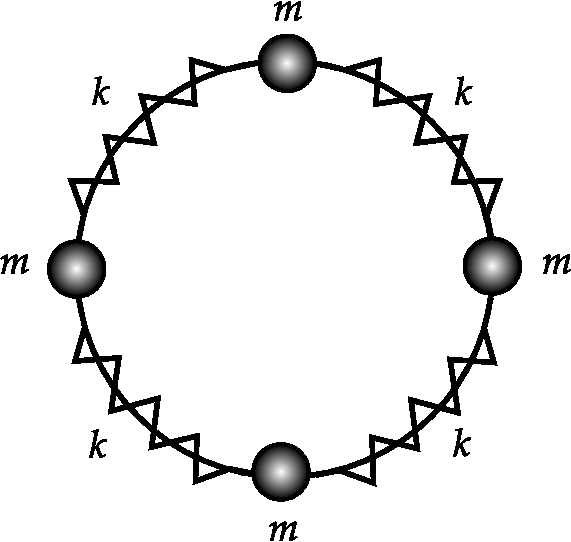
\includegraphics[height=4.8cm,width=5cm]{small oscillations-01}
		\end{figure}
		\begin{align*}
		\intertext{we find the equations of motion:}
		\frac{d}{d t} \frac{\partial L}{\partial \dot{\varphi}_{v}}=m R \ddot{\varphi}_{v}=-\frac{1}{2} k R^{2}\left[2\left(\varphi_{v}-\varphi_{v+1}\right)+2\left(\varphi_{v}-\varphi_{v+1}\right)\right]&=\frac{\partial L}{\partial \varphi_{v}} .
	\intertext{	For the case of four mass points, we then obtain}
	\ddot{\varphi}_{1}=\frac{k}{m}\left(\varphi_{2}-2 \varphi_{1}+\varphi_{4}\right), \quad \ddot{\varphi}_{2}&=\frac{k}{m}\left(\varphi_{3}-2 \varphi_{2}+\varphi_{1}\right)\\
	\ddot{\varphi}_{3}=\frac{k}{m}\left(\varphi_{4}-2 \varphi_{3}+\varphi_{2}\right), \ddot{\varphi}_{4}&=\frac{k}{m}\left(\varphi_{1}-2 \varphi_{4}+\varphi_{3}\right)
	\intertext{With the ansatz $\varphi_{v}=A_{v} \cos \omega t, \ddot{\varphi}_{v}=-A_{v} \omega^{2} \cos \omega t$, we are led to the following linear system of equations:}
	\left(\begin{array}{cccc}2 \frac{k}{m}-\omega^{2} & -\frac{k}{m} & 0 & -\frac{k}{m} \\ -\frac{k}{m} & 2 \frac{k}{m}-\omega^{2} & -\frac{k}{m} & 0 \\ 0 & -\frac{k}{m} & 2 \frac{k}{m}-\omega^{2} & -\frac{k}{m} \\ -\frac{k}{m} & 0 & -\frac{k}{m} & 2 \frac{k}{m}-\omega^{2}\end{array}\right)\left(\begin{array}{l}A_{1} \\ A_{2} \\ A_{3}\end{array}\right)&=0
	\intertext{For the nontrivial solutions, the determinant of the coefficient matrix must vanish. This condition leads to the determining equation for the eigenfrequencies:}
	\left(2 \frac{k}{m}-\omega^{2}\right)^{2}\left(4 \frac{k}{m}-\omega^{2}\right)\left(-\omega^{2}\right)=0
	\intertext{The frequencies are}
	\omega_{1}^{2}=0, \quad \omega_{2}^{2}&=4 \frac{k}{m}, \quad \omega_{3}^{2}=\omega_{4}^{2}=2 \frac{k}{m}
\intertext{	To calculate the related eigenvibrations, we insert these frequencies into the system of equations:}
	\end{align*}
\begin{align*}
	&\text{(1) }\omega_{1}^{2}=0: A_{1}=A_{2}=A_{3}=A_{4} : \text{The system does not vibrate but performs a uniform rotation}\\
	&\text{(2) }\omega_{2}^{2}=4 \frac{k}{m}: A_{1}=A_{3}=-A_{2}=-A_{4}:\text{ Two neighboring mass points perform an out-of-phase vibration}\\
	&\text{(3) }\omega_{3}^{2}=\omega_{4}^{2}=2 \frac{k}{m}: A_{1}=A_{2}=-A_{3}=-A_{4}\text{ or }A_{1}=A_{4}=-A_{2}=-A_{3} :\text{ Two neighboring mass points }\\&\text{vibrate in phase}
	\end{align*}
	\begin{figure}[H]
		\centering
		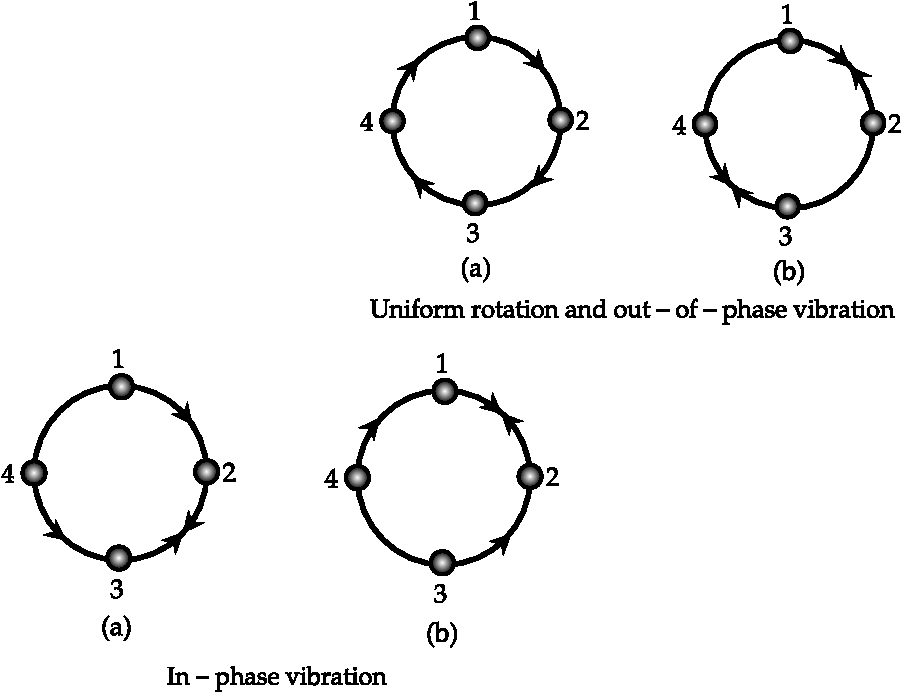
\includegraphics[height=8cm,width=11cm]{small oscillations-02}
	\end{figure}
	\end{answer}
	\item Two equal masses coupled by two equal springs
	Two equal masses move without friction on a plate. They are connected to each other and to the wall by two springs, as is indicated by Figure $7.3$. The two spring constants are equal, and the motion shall berestricted to a straight line (one-dimensional motion).
	Find\\
	(a) the equations of motion,\\
	(b) the normal frequencies, and\\
	(c) the anplitude ratios of the normal vibrations and the general solution.
	\begin{answer}
		\begin{align*}
		\intertext{(a) Let $x_{1}$ and $x_{2}$ be the displacements from the rest positions. The cquations of motion then read}
		m \ddot{x}_{1}&=-k x_{2}+k\left(x_{2}-x_{1}\right) \\
		m \dot{x}_{2}&=-k\left(x_{2}-x_{1}\right)
		\intertext{(b) For determining the normal frequencies, we use the ansatz}
		x_{1}&=A_{1} \cos \omega t, \quad x_{2}=A_{2} \cos \omega t
		\end{align*}
		\begin{figure}[H]
			\centering
			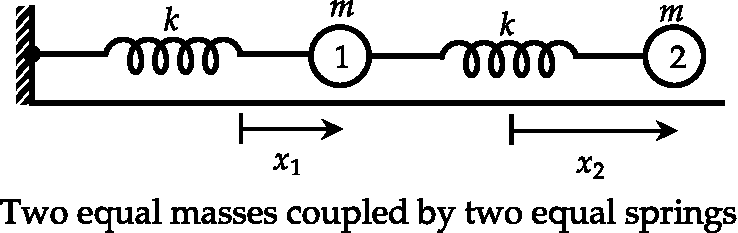
\includegraphics[height=2cm,width=6.5cm]{small oscillations-03}
		\end{figure}
		\begin{align}
	\intertext{	and thereby get from $\color{red}{(7.9)}$ and $(\color{red}{7.10})$ the equations}\notag\\
		&\left(2 k-m \omega^{2}\right) A_{1}-k A_{2}=0 \label{so-05}\\
		&-k A_{1}+\left(k-m \omega^{2}\right) A_{2}=0\notag
		\intertext{From therequirement for nontrivial solutions of the system of equations, it follows that the determinant of coefficient vanishes:}\notag
		D&=\left|\begin{array}{cc}
		2 k-m \omega^{2} & -k \notag\\
		-k & k-m \omega^{2}
		\end{array}\right|=0
	\intertext{	From this follows the determining equation for the eigenfrequencies,}\notag
		\omega^{4}-3 \frac{k}{m} \omega^{2}+\frac{k^{2}}{m^{2}}&=0\notag
		\intertext{with the positive solutions}\notag
		\omega_{1}=\frac{\sqrt{5}+1}{2} \sqrt{\frac{k}{m}} \text { and } \omega_{2}&=\frac{\sqrt{5}-1}{2} \sqrt{\frac{k}{m}}, \omega_{1}>\omega_{2} .\notag
		\intertext{By inserting the eigenfrequencies in (\ref*{so-05}) one sees that the higher frequency $\omega_{1}$ corresponds to the oppositephase mode, and the lower frequency $\omega_{2}$ to the equal-phase normal vibration:}\notag
		\text{with }\omega_{1}^{2}&=\frac{1}{2}(3+\sqrt{5}) \frac{k}{m}, \quad\text{ it follows from (\ref{so-05}) that }A_{2}=-\frac{\sqrt{5}-1}{2} A_{1}\notag\\ \text{with }\omega_{2}^{2}&=\frac{1}{2}(3-\sqrt{5}) \frac{k}{m},\text{ it follows from (\ref{so-05}) that }A_{2}=\frac{\sqrt{5}+1}{2} A_{1} .\notag
		\intertext{Since the two mass points are fixed in different ways, we find amplitudes of different magnitudes. The general solution is obtained as a superposition of the normal vibrations, using the calculated amplitudes ratios:}\notag
		x_{1}(t)&=C_{1} \cos \left(\omega_{1} t+\varphi_{1}\right)+C_{2} \cos \left(\omega_{2} t+\varphi_{2}\right)\notag\\
		x_{2}(t)&=-\frac{\sqrt{5}-1}{2} C_{1} \cos \left(\omega_{1} t+\varphi_{1}\right)+\frac{\sqrt{5}+1}{2} C_{2} \cos \left(\omega_{2} t+\varphi_{2}\right)\notag
		\end{align}
	\end{answer}
	\item  The Lagrangian of a system is given by $L=\frac{1}{2} m \dot{q}_{1}^{2}+2 m \dot{q}_{2}^{2}-k\left(\frac{5}{4} q_{1}^{2}+2 q_{2}^{2}-2 q_{1} q_{2}\right)$ where $m$ and $k$ are positive constants. The frequencies of its normal modes are
 \begin{tasks}(2)
	\task[\textbf{a.}]$\sqrt{\frac{k}{2 m}}, \sqrt{\frac{3 k}{m}}$
	\task[\textbf{b.}]$\sqrt{\frac{k}{2 m}}(13 \pm \sqrt{73})$
	\task[\textbf{c.}]$\sqrt{\frac{5 k}{2 m}}, \sqrt{\frac{k}{m}}$
	\task[\textbf{d.}]  $\sqrt{\frac{k}{2 m}}, \sqrt{\frac{6 k}{m}}$
\end{tasks}
	\begin{answer}
		\begin{align*}
		 L &=\frac{1}{2} m \dot{q}_{1}^{2}+2 m \dot{q}_{2}^{2}-k\left(\frac{5}{4} q_{1}^{2}+2 q_{2}^{2}-2 q_{1} q_{2}\right) \\ &=\frac{1}{2} m \dot{q}_{1}^{2}+\frac{1}{2} 4 m \dot{q}_{2}^{2}-\frac{1}{2} k\left(\frac{5}{2} q_{1}^{2}+4 q_{2}^{2}-4 q_{1} q_{2}\right) \\ \hat{T} &=\left(\begin{array}{cc}m & 0 \\ 0 & 4 m\end{array}\right), \hat{V}=\left(\begin{array}{cc}\frac{5}{2} k & -2 k \\ -2 k & 4 k\end{array}\right) 
		 \intertext{For frequencies of normal modes:}
		 \operatorname{det}\left|\omega^{2} \hat{T}-\hat{V}\right|&=0\\
		 \left|\begin{array}{cc}\left(m \omega^{2}-\frac{5}{2} k\right) & 2 k \\ 2 k & \left(4 m \omega^{2}-4 k\right)\end{array}\right|&=0 \Rightarrow 4\left(m \omega^{2}-k\right) \frac{\left(2 m \omega^{2}-5 k\right)}{2}-4 k^{2}=0\\
		 \Rightarrow 2 m^{2} \omega^{4}+5 k^{2}-7 k m \omega^{2}-2 k^{2}&=0\\
		 \Rightarrow 2\left(m \omega^{2}\right)^{2}-7 k\left(m \omega^{2}\right)+3 k^{2}&=0\\
		 \Rightarrow m \omega^{2}&=\frac{7 k \pm \sqrt{49 k^{2}-24 k^{2}}}{4}=\frac{7 k \pm \sqrt{49 k^{2}-24 k^{2}}}{4}\\&=\frac{7 k \pm 5 k}{4}=3 k, \frac{k}{2}\\
		 \therefore \omega&=\sqrt{\frac{3 k}{m}}, \sqrt{\frac{k}{2 m}}
		\end{align*}
		 Correct answer is option \textbf{(a)}
	\end{answer}
	
	
	
	
	
	
	
	
	
	
	
	
	
	
	
	
	
\end{enumerate}
%\chapter{VECTOR ALGEBRA}

\begin{definition}
A vector is defined as a physical quantity having magnitude and a direction associated with it. 
\end{definition}
\begin{example}
	 Displacement,Velocity, Acceleration, Force ,Torque,Angular momentum etc. 
\end{example}
\section{Vector representation}
Geometrically  a  vector  is  represented  by  a  directed  line  segment, with length proportional to the magnitude.The direction of the arrow gives the direction of the vector.\newline
We will refer to the start of the arrow as the tail and the end as the tip or head. The vector between two points P and Q  will be denoted as, $\overrightarrow{\mathrm{P Q}}$(or by a boldface $\mathbf{PQ}$). And the  magnitude as $|\mathrm{ PQ}| .$  Magnitude will also be called length or norm.\\\\ Analytically a three  dimensional  vector  can  be  specified  by  an  ordered  set  of  three  numbers,  called  its  components.The magnitude  of  the  components  depend  on  the  coordinate  system  used. (A vector can be extended to $n$ dimensions). A vector $\vec{A}$ is represented by $\left(A_{x}, A_{y}, A_{z}\right)$ in cartesian (rectangular) coordinate system .\\Magnitude of vector $\vec{\mathrm A}$ is given by, $|\vec{\mathrm A}|=\sqrt{\mathrm A_{x}^{2}+\mathrm A_{y}^{2}+\mathrm A_{z}^{2}}$
\subsection{Position vector:} 
\begin{definition}
	Vectors that start at the origin and terminate at any arbitrary point are called position vectors. These are used to determine the position of a point with reference to the origin.
\end{definition}
\begin{figure}[H]
	\centering
	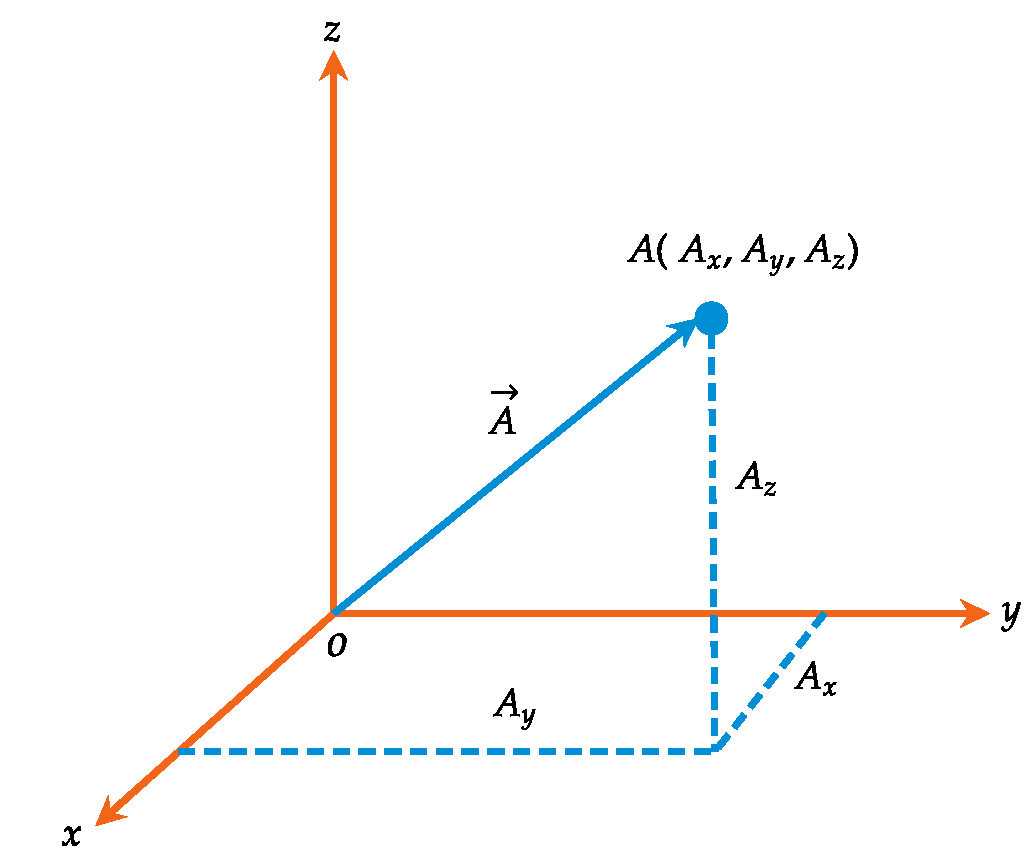
\includegraphics[width=0.4\textwidth]{vector2}
	\caption{Representation of position vector $\vec{A }$}
\end{figure}
 Any vector $\vec{\mathrm A}$ in the $3-\mathrm{\mathrm D}$ right handed rectangular cartesian coordinate system can be represented as,
 \begin{equation}
$$\vec{\mathrm A}=\mathrm A_{x} \hat{i}+\mathrm A_{y} \hat{j}+\mathrm A \hat{k}$$
 \end{equation} 
Where, $\hat{i}, \hat{j}$ and $\hat{k}$ are the unit vectors in direction of $x, y$ and $z$ axis respectively. $\mathrm A_{x}, \mathrm A_{y} $ and $ \mathrm A_{z}$ are the
cartesian components or projections of vector $\vec{A}$ along $x, y, z$ axis.
 \begin{exercise}
	 If $\mathrm A$ and $\mathrm B$ are (3,4,5) and $(6,8,9),$ find $\vec {\mathrm {A B}}$.
	\end{exercise}
\begin{answer}
$$\begin{aligned} \overrightarrow{\mathrm {A B}} &=\text { Position vector of } \mathrm B-\text { Position vector of } \mathrm A \\ &=(6 \hat{i}+8 \hat{j}+9 \hat{k})-(3 \hat{i}+4 \hat{j}+5 \hat{k}) \\ &=3 \hat{i}+4 \hat{j}+4 \hat{k} \end{aligned}$$
\end{answer}

\subsection{Unit vector:} 
\begin{definition}
	A vector quantity having unit magnitude is called unit vector.A unit vector along $\vec{A}$ is defined as,
	\\$\hat{\mathrm A}=\frac{\vec{\mathrm A}} {|\vec{\mathrm A}|}=\frac {\left(\mathrm A_{x} \hat{i}+\mathrm A_{y} \hat{j}+\mathrm A_{z} \hat{k}\right) } {\sqrt{\mathrm A_{x}^{2}+\mathrm A_{y}^{2}+\mathrm A_{z}^{2}}}$
\end{definition}
 \begin{exercise}
 	Find unit vector in the direction of vector $\vec{a}=2 \hat{i}+3 \hat{j}+\hat{k}$
 	 \end{exercise}
  \begin{answer}
  	
  	\begin{align*}
  		\text{Magnitude of }\vec{ a}&=\sqrt{2^{2}+3^{2}+1^{2}}\\
  		|\vec{a}|&=\sqrt{4+9+1}=\sqrt{14}\\
  		\text{Unit vector in direction of }\vec{a}&=\frac{\vec{a}}{| \vec{a}|}\\
  		\hat{a}&=\frac{1}{\sqrt{14}}[2 \hat{i}+3 \hat{j}+1 \hat{k}] \\
  		\hat{a}&=\frac{2}{\sqrt{14}} \hat{i}+\frac{3}{\sqrt{14}} \hat{i}+\frac{1}{\sqrt{14}} \hat{k}
  	\end{align*}
  	
  \end{answer}
  \subsection{Direction cosines}
In analytical geometry the direction cosines are the angles made by the vector with  the three coordinate axes.\\\\\textbf{Direction cosines of vector $\vec{\mathrm A}$} :
\\\newline If $\vec{\mathrm A}$ makes angles $\alpha, \beta, \gamma$ with $x, y$ and $z$ axes respectively, then direction cosines of $\vec{\mathrm A}$ are defined as,
\begin{minipage}{0.6\textwidth}
	\begin{flalign*}
	&l=\cos \alpha=\frac{\mathrm A_{x}}{\mathrm A}\quad ;\quad  m=\cos \beta=\frac{\mathrm A_{y}}{\mathrm A} \quad ;\quad  n=\cos \gamma=\frac{\mathrm A_{z}}{\mathrm A} \\  &l^{2}+m^{2}+n^{2}=1\\\\
	&\text{Then the unit vector along } \vec{\mathrm A}\text{ can be written as,}\\
	& \hat{\mathrm A}=l \hat{i}+m \hat{j}+n \hat{k}\\
	\end{flalign*}
\end{minipage}
\begin{minipage}{0.4\textwidth}
	\begin{figure}[H]
		\centering
		\includegraphics[width=6cm,height=6cm]{direction cosine}\caption{Direction cosine.}
	\end{figure}
\end{minipage}
\section{Types of vectors}
\begin{itemize}
	\item \textbf{{Equal vectors}}\hspace{0.74cm}\textbf{:}\quad Vectors having same magnitude and same direction.
	\item \textbf{Null Vectors }\hspace{0.82cm}\textbf{:} \quad Vectors having coincident initial and terminal point i.e its magnitude is zero and it has any arbitrary direction.
	\item \textbf{Reciprocal Vector }\textbf{:}\quad Vector having same direction as $\vec{\mathrm  A}$ but magnitude reciprocal to that of $\vec{\mathrm A},$ is known as the reciprocal vector of $\mathrm A$ Reciprocal vector of $\vec{\mathrm A}$ is $\vec{\mathrm A}-\frac{1}{\mathrm A} \hat{\mathrm A}$.
	\item \textbf{Negative Vector}\hspace{0.3cm} \textbf{:}\quad Vectors having same magnitude as $\vec{\mathrm a}$ but direction opposite to that of $\vec{\mathrm A},$ is known
	as the negative vector of $\vec{\mathrm a} .$ Negative vector as $\vec{\mathrm A}$ is $-\vec{\mathrm A}=-|\mathrm A| \hat{\mathrm A}$.
\end{itemize}
\section{Vector operations}\index{Vector operations}
\subsection{Vector addition}
\begin{itemize}
	\item 	\textbf{Triangular law of vector addition:}
	\begin{itemize}
		\item Place the tail of $\vec{\mathrm A}$ at the head of $\vec{\mathrm B} $.
		\item The resultant vector $\vec{\mathrm A}+\vec{\mathrm B}$ is formed by connecting the tail of the first vector to the head of the last vector. 
	\end{itemize}
\begin{figure}[H]
	\begin{minipage}{0.45\textwidth}
		\centering
		\includegraphics[width=0.70\textwidth]{Triangular}
		\caption{Triangular law of vector addition}
		\end{minipage}\hfil
	\begin{minipage}{0.45\textwidth}
	\centering
	\includegraphics[width=0.75\textwidth]{parellelogram}
	\caption{Parellelogram law of vector addition}
\end{minipage}

\end{figure}

\item \textbf{Parellelogram law of vector addition:}
\\ \\When two vectors act at a point, their resultant is found by the law of parallelogram of vectors.(We got to use it often in Electricity and magnetism.)

The magnitude of Resultant vector ${\vec{A }+\vec{B}}$
From right angled $\triangle$ OCD.
\begin{align*}
O C^{2}&=O D^{2}+C D^{2}\\
&=(O A+AD)^{2}+C D^{2}\\
&=O A^{2}+A D^{2}+2AD\cdot OA +C D^{2}\\\\
\text{Here,}\hspace{1.3cm} O A&= A\ ; \ AD=B\cos\theta \ ; \ CD= B\sin\theta\\\\
\text{Then,}\hspace{1.1cm}  O C^{2}&=|\vec{A }+\vec{B}|^{2}\\&=A^{2}+(B\cos\theta)^{2}+(B\sin\theta)^{2}+2AB\cos\theta\\&=A^{2}+B^{2}+AB\cos\theta\\
|\vec{A }+\vec{B}|&=\sqrt{A^{2}+B^{2}+2AB\cos\theta}\\
\\
\text{The direction of }&\text{ Resultant vector}\ {\vec{A }+\vec{B}} \ \text{with the vector}  \ {\vec{A}}\\
\tan \alpha&=\frac{B \sin \theta}{A+B \cos \theta}\\
\alpha&=\tan ^{-1}\left(\frac{B \sin \theta}{A+B \cos \theta}\right)\\
\text{If the  two vectors}&\text{   are parellel i.e., $\theta=0$ \ Then,  }\ \\
|\vec{A }+\vec{B}|&=\sqrt{A^{2}+B^{2}+2AB}=\sqrt{(A+B)^{2}}=(A+B)\\
\text{If the  two vectors}&\text{   are anti-parellel i.e., $\theta=180$ \ Then,  }\ \\
|\vec{A }+\vec{B}|&=\sqrt{A^{2}+B^{2}-2AB}=\sqrt{(A-B)^{2}}=(A-B)\\
\end{align*}
\end{itemize}
\begin{note}
	\leavevmode
	\\\\
     	If $|\vec{A}|=|\vec{B}|=A$ Then resultant of these two vectors will be,
	\begin{enumerate}
		\item $\theta=0\qquad \rightarrow \sqrt{A^{2}+A^{2}+2A A\cos 0} \hspace{0.2cm}=\sqrt{A^{2}+A^{2}+2A^{2}}=2A $ 
		\item $\theta=60^{\circ} \quad\rightarrow \sqrt{A^{2}+A^{2}+2A A\cos 60}=\sqrt{A^{2}+A^{2}+A^{2}} =\sqrt{3}A $
		\item $\theta=90^{\circ}\quad\rightarrow \sqrt{A^{2}+A^{2}+2A A\cos 90}=\sqrt{A^{2}+A^{2}}=\sqrt{2} A $
			\item $\theta=180^{\circ} \hspace{0.3cm} \rightarrow \sqrt{A^{2}+A^{2}+2A A\cos 180}=\sqrt{A^{2}+A^{2}-2A^{2}} =0 $ 
	\end{enumerate}
\end{note}

\subsubsection{Properties of vector addition}
\begin{itemize}
	\item Commutation property:
	$\mathbf{A}+\mathbf{B}=\mathbf{B}+\mathbf{A}$.
	\item Associative property:$(\mathbf{A}+\mathbf{B})+\mathbf{C}=\mathbf{A}+(\mathbf{B}+\mathbf{C})$.
	\item Additive identity:$\mathbf{A}+\mathbf{0}=\mathbf{A} \quad$.
	\item Additive inverse:$\mathbf{A}+(-\mathbf{A})=\mathbf{0} \quad$ .
	
\end{itemize}
\subsection{Vector  multiplication}
\subsubsection{\large{1}.{Scaling of vector}(Multiplication by scalar)}
Scaling a vector means changing it's length by a scale factor.	Multiplication of a vector by a positive scalar $'c'$, multiplies the magnitude but leaves the
direction unchanged. If $'c'$ is negative, the direction is reversed.
\begin{figure}[H]
	\begin{center}
		\includegraphics[width=0.30\textwidth]{scaling}
	\end{center}
\caption{Scaling of vector}
\end{figure}
\subsubsection{Properties of scalar multiplication}
\begin{itemize}
	\item  Distributive property:\quad$a(\vec{\mathrm A}+\vec{\mathrm B})=a \vec{\mathrm A}+a \vec{\mathrm B}$.
\end{itemize}
\subsubsection{\large{2}.Dot product or scalar product of two vectors}
The dot product of two vectors is defined as
\begin{equation}
$$\vec{A} \cdot \vec{B}=|A| | B| \cos \theta$$
\end{equation}
Where $\theta$ is the angle they form when placed tail to tail. $\vec{\mathrm{A}} \cdot \vec{\mathrm B}$ is itself a scalar.Geometrically $\vec{\mathrm A} \cdot \vec{\mathrm B}$ is the product of $\mathrm A$ times the projection of $\vec{\mathrm B}$ along $\vec{\mathrm A}$.
\\\newline In general,\ If \ $\vec{\mathrm A}=\mathrm A_{z} \hat{i}+\mathrm A_{y} \hat{j}+\mathrm A_{z} \hat{k}$ and $\vec{\mathrm B}=\mathrm B_{x} \hat{i}+\mathrm B_{y} \hat{j}+\mathrm B_{z} \hat{k},$\\\\ Then we can construct the scalar product of $\vec{\mathrm A}$ and $\vec{\mathrm B}$ as,
\begin{equation}
$$\vec{\mathrm A} \cdot \vec{ \mathrm B}=\mathrm A_{x} \mathrm B_{x}+\mathrm A_{y} \mathrm B_{y}+\mathrm A_{z} \mathrm B_{z}$$
\end{equation}  
\begin{example}\textbf{Workdone:}
	If a constant force $F$ acting on a particle displaces it from the point A to B then,\\
	\begin{minipage}{0.45\textwidth}
		\begin{align*}
		\text{Work done} &=\text{(component of F along A B ). Displacement}\\
		&=\mathrm{F} \cos \theta . A B \\
		&=\vec{F} \cdot \overrightarrow{A B}\\
		\text{Work done }&=\text{Force. Displacement}
		\end{align*}
	\end{minipage}
	\begin{minipage}{0.45\textwidth}
	\begin{figure}[H]
		\begin{center}
			\includegraphics[width=0.65\textwidth]{workdone}
		\end{center}
		\caption{Workdone}
	\end{figure}
\end{minipage}
\end{example}
\subsubsection{Projection:}Projection of a vector A on B is the component of vector A in the direction of vector B.$$\text{Projection of}\quad \vec{\mathrm A} \text{\quad along}\quad \vec{\mathrm B} =\vec{\mathrm A}\cos\theta =\vec{\mathrm A} \cdot \hat{\mathrm B}$$.
\subsubsection{Properties of Dot product}
\begin{itemize}
	\item Commutative property:$\vec{\mathrm A} \cdot \vec{\mathrm B} =\vec{\mathrm B} \cdot \vec{\mathrm A}$.
	\item Asociative property:$ \vec{\mathrm A} \cdot(\vec{\mathrm B}+\vec{\mathrm C}) =\vec{\mathrm A} \cdot \vec{\mathrm B}+\vec{\mathrm A} \cdot \vec{\mathrm C}$.
	\item For two mutually perpendicular vectors $\vec{\mathrm A}$ and $\mathrm B, \mathrm A \cdot \vec{\mathrm B}=0$.
	\item If the two vectors are parallel, $\vec{\mathrm A} \cdot \vec{\mathrm B}=\mathrm {A B}$.(since, $\cos0=1$)
	\item $\hat{i} \cdot \hat{j}=\hat{j} \cdot \hat{k}=\hat{k} \cdot i=0\newline  \hat{i} \cdot \hat{i}=\hat{j}\cdot\hat{j} = \hat{k}\cdot \hat{k}=1$\\\\ 
\end{itemize}
\begin{exercise}
	For the two vectors  $ \vec{A}=6\hat{i}+4\hat{j}+3\hat{k}$ and $ \vec{B}=2\hat{i}-3\hat{j}-3\hat{k}$
	\newline  $$\begin{aligned}
	\vec{\mathrm A} \cdot \vec{ \mathrm B}&=\mathrm A_{x} \mathrm B_{x}+\mathrm A_{y} \mathrm B_{y}+\mathrm A_{z} \mathrm B_{z}\\
	&=12-12-9\\
	&=-9
	\end{aligned}$$
\end{exercise}
\subsubsection{{\large 3}.Vector  product or Cross product}
Cross product of two vectors $\vec{\mathrm A}$ and $\vec{\mathrm B}$  is defined as a vector that is perpendicular (orthogonal) to both $\vec{\mathrm A}$ and $\vec{\mathrm B}$, with  a magnitude equal to the area of the parallelogram that the vectors span(This suggest that area may be treated as a vector quantity). Since there are two opposite directions which are so perpendicular to $\vec{A} \ \text{and} \ \vec{B}$  This does not uniquely determine $\vec{A} \times \vec{B}$ . The direction of $\vec{A} \times \vec{B}$ is fixed by a convention, called the Right Hand Rule.\\\\
\textbf{Right Hand Rule :}\\
Stretch out the fingers of the right hand so that the thumb becomes perpendicular to both the index (fore
finger) and the middle finger. If the index points in the direction of $\vec{A}$ and the middle finger in the direction of
$\vec{B}$ then, $\vec{A} \times \vec{B}$ points in the direction of the thumb.\\\\
The vector product of $\vec{A} \ \text{and} \ \vec{B}$  is defined as, 
\begin{equation}
$$\vec{\mathrm A} \times \vec{\mathrm B}=|\vec{\mathrm A}||\vec{\mathrm B}| \sin \theta  \hat{n}$$
\end{equation}
Where $\hat{n}$ is unit vector normal to the plane containing $\vec{\mathrm A}$ and $\vec{\mathrm B}$.
\\Using decomposition of vector into their cartesian components,we can find $\vec{\mathrm A} \times \vec{\mathrm B}$ as,
\\ If $\vec{\mathrm A}=\mathrm A_{z} \hat{i}+\mathrm A_{y} \hat{j}+\mathrm A_{z} \hat{k}$ and $\vec{\mathrm B}=\mathrm B_{x} \hat{i}+\mathrm B_{y} \hat{j}+\mathrm B_{z} \hat{k},$ then $$\vec{\mathrm A} \times \vec{\mathrm B}=\left|\begin{array}{lll}\hat{i} & \hat{j} & \hat{k} \\ \mathrm A_{x} & \mathrm A_{y} & \mathrm A_{z} \\ \mathrm B_{x} & \mathrm B_{y} & B_{z}\end{array}\right|$$
\begin{example}
	Angular momentum
	\newline The angular momentum of a particle, about a reference point , is defined as the vector product of the potion relative to the reference point, and momentum of the particle
	 $$ L=r\times p$$
	 \begin{figure}[H]
	 	\begin{center}
	 		\includegraphics[width=0.30\textwidth]{angular momentum}
	 	\end{center}
 	\caption{Angular momentum}
	 \end{figure}
\end{example}
\subsubsection{Properties of Cross product} 
\begin{itemize}
	\item Distributive property\hspace{0.7cm}:\ $\vec{\mathrm A} \times(\vec{\mathrm B} + \vec{\mathrm C})=(\vec{\mathrm A} \times \vec{\mathrm B})+(\vec{\mathrm A} \times \vec{\mathrm C})$
	\item Commutative property\quad:\ $\vec{\mathrm A} \times \vec{\mathrm B}=-(\vec{\mathrm B} \times \vec{\mathrm A})$.
	\item For two collinear vectors (parallel or anti-parallel vectors) $\vec{\mathrm A} \times \vec{\mathrm B}=0$.
	\item $\hat{i} \times \hat{i}=\hat{j} \times \hat{j}=\hat{k} \times \hat{k}=0\\\\
	\; \ \hat{i} \times \hat{j}=\hat{k}
	\; \ \hat{j} \times \hat{k}=\hat{i}
	\; \ \hat{k} \times \hat{i}=\hat{j}$.
	
\end{itemize}
\begin{exercise}
	Find the area of a parallelogram whose adjacent sides are $\hat{i}-2 \hat{j}+3 \hat{k}$ and
	$2 \hat{i}+\hat{j}-4 \hat{k}$.
\end{exercise}
\begin{answer}
	\begin{align*}
\text{Vector area of parellelogram}&=\left|\begin{array}{rrr}\hat{i} & \hat{j} & \hat{k} \\ 1 & -2 & 3 \\ 2 & 1 & -4\end{array}\right|\\
&=(8-3) \hat{i}-(-4-6) \hat{j}+(1+4) \hat{k}=5 \hat{i}+10 \hat{j}+5 \hat{k}\\
\text{Area of parallelogram}&=\sqrt{(5)^{2}+(10)^{2}+(5)^{2}}=5 \sqrt{6}
\end{align*}
\end{answer}


\subsubsection{4.Triple product}
\begin{itemize}
	\item \textbf{Scalar Triple product}
	\\The scalar triple product of three vectors $\vec{\mathrm{A}}, \vec{\mathrm{B}}$, and $\vec{\mathrm{C}}$ is $(\vec{\mathrm{A}} \times\vec{\mathrm{B}}) \cdot \vec{\mathrm{C}} .$ It is a scalar product because, just like the dot product, it evaluates to a single number.  The absolute value of $|(\vec{\mathrm{A}} \times \vec{\mathrm{B}}) \cdot \vec{\mathrm{C}}|$ is the volume of the parallelepiped spanned by $\vec{\mathrm{A}}, \vec{\mathrm{B}},$ and $\vec{\mathrm{C}}$ (i.e., the parallelepiped whose adjacent sides are the vectors $\vec{\mathrm{A}}, \vec{\mathrm{B}},$ and $\vec{\mathrm{C}}$ ).\begin{figure}[H]
		\begin{center}
			\includegraphics[width=0.25\textwidth]{parellelopiped}
		\end{center}
	\caption{Scalar triple product}
	\end{figure}
\begin{align*}
	\vec{\mathrm A} \cdot(\vec{\mathrm B} \times \vec{\mathrm C})&=\vec{\mathrm B} \cdot(\vec{\mathrm C} \times \vec{\mathrm A})=\vec{\mathrm C} \cdot(\vec{\mathrm A} \times \vec{\mathrm B})\\
	\text{In component form}\ \vec{\mathrm A} \cdot(\vec{\mathrm B} \times \vec{\mathrm C})&=\left|\begin{array}{lll}\mathrm A_{x} & \mathrm A_{y} & \mathrm A_{z} \\ \mathrm B_{x} & \mathrm B_{y} & \mathrm B_{z} \\ \mathrm C_{x} & \mathrm C_{y} & \mathrm C_{z}\end{array}\right|\\
\end{align*}

	\item \textbf{Vector Triple product}
	\\A vector triple product $\vec{\mathrm A} \times(\vec{\mathrm B} \times \vec{\mathrm C})$ of 3 vectors ,$\vec{\mathrm A}$ , $\vec{\mathrm B}$ and $\vec{\mathrm C}$ is simply a vector lying in the plane containing $\vec{\mathrm A}$ , $\vec{\mathrm B}$ and $\vec{\mathrm C}$.\\

	The vector triple product can be simplified by the so-called $\text{ B A C}-\text{ C A B}$ rule.The equation is linear in  A,B and C.
	$$
	\vec{\mathrm A} \times(\vec{\mathrm B} \times \vec{\mathrm C})=\vec{\mathrm B}(\vec{\mathrm A} \cdot \vec{\mathrm C})-\vec{\mathrm C}(\vec{\mathrm A} \cdot \vec{\mathrm B})
	$$
\end{itemize}
\begin{note}

Suppose we have two vectors $ \vec{a}$ and $ \vec {b}$ as shown in the figure.
\ref{vector}
We can write $\vec{b}$ as
$$\vec{b}=\vec{{b_{\parallel}}}+\vec{{b_{\perp}}} $$
Where ${b_{\parallel}}$ is the projection of $ \vec {b}$ along  $ \vec{a}$ and$ \vec{{b_{\perp}}}$ is the projection of  $ \vec {b}$ perpendicular to $ \vec{a}$\\
\begin{minipage}{0.65\textwidth}
	\begin{align*}
	\vec {b}=&(\vec{b}\cdot \hat{a})\cdot \hat{a}+\vec{{b_{\perp}}}\\
	\vec {b}=&\frac{(\vec{b}\cdot \vec{a})\cdot\vec{a}}{a^{2}}+\vec{{b_{\perp}}}\\
	\vec {b}=&\frac{(\vec{b}\cdot \vec{a})\cdot\vec{a}}{a^{2}}+{\vec{b}-\frac{(\vec{b}\cdot \vec{a})\cdot\vec{a}}{a^{2}}}\\
	\vec {b}=&\frac{(\vec{b}\cdot \vec{a})\cdot\vec{a}}{a^{2}}+\frac{\vec{b}(\vec{a}\cdot\vec{a})-{(\vec{b}\cdot\vec{a})\vec{a}}}{a^{2}}\\
	\vec {b}=&\frac{(\vec{b}\cdot \vec{a})\cdot\vec{a}}{a^{2}}+\frac{\vec{a}\times(\vec{b}\times\vec{a})}{a^{2}}\\
	\vec{b}=&\vec{{b_{\parallel}}}(\text{parellell component})+\vec{{b_{\perp}}}(\text{perpendicular component})
	\end{align*}
\end{minipage}
\begin{minipage}{0.35\textwidth}\hfill
\begin{figure}[H]
	\begin{center}
		\includegraphics[width=0.8\textwidth]{vector1}
	\end{center}
\caption{vector}
\label{vector}
\end{figure}
\end{minipage}
\end{note}

\section{General curvilinear coordinate system}\index{General culvilinear coordinate system}
Not all Physical problems  are well adapted to a solution in cartesian coordinate system.We have to develop a general system that may be apt for any particular system of intersect.
The coordinates in general curvilinear coordinate system be described by three coordinates, $q_{1},q_{2} $ and $ q_{3}$\\then  a position vector $ \vec{ r}$ in the system can be represented as,
\begin{align*}
\vec{r}&=\vec{r}(q_{1},q_{2},q_{3})\\
\text{Then,}\quad
 dr&={\frac{\partial r}{\partial q_{1} }} dq_{1}+{\frac{\partial r}{\partial q_{2} }} dq_{2}+{\frac{\partial r}{\partial q_{3} }} dq_{3}
\end{align*}
Where,\ ${\frac{\partial r}{\partial q_{1} }}$,${\frac{\partial r}{\partial q_{2} }}$,${\frac{\partial r}{\partial q_{3} }}$ are the tangent vectors along $q_{1},q_{2}  $ and \ $q_{3}$.
\\\\The unit vectors along $q_{1},q_{2}  $ and \ $q_{3}$ are defined as,
$$ \hat e_{1}=\frac{{\frac{\partial r}{\partial q_{1} }}}{|{\frac{\partial r}{\partial q_{1} }}|}\quad ;\quad
 \hat e_{2}=\frac{{\frac{\partial r}{\partial q_{2} }}}{|{\frac{\partial r}{\partial q_{2} }}|}\quad ;\quad\hat e_{3}=\frac{{\frac{\partial r}{\partial q_{3} }}}{|{\frac{\partial r}{\partial q_{3} }}|}$$
\\
\textbf{Scaling factor:}\\\\
The factor ${|{\frac{\partial r}{\partial q_{1} }}|}$ is known as the scaling factor. It is denoted as $h_{1}$.\\\\
Similiarly, $h_{2}={|{\frac{\partial r}{\partial q_{2} }}|}$
and $h_{3}={|{\frac{\partial r}{\partial q_{3} }}|}$\\
\\Then the position vector can be written as,
\begin{equation}
$$ \vec dr=h_{1}\hat e_{1} dq_{1}+h_{2}\hat e_{2} q_{2}+h_{3}\hat e_{3}q_{3}$$
\end{equation}
\textbf{Cartesian coordinate system}
\begin{alignat*}{4}
&\text{Coordinates}&& \textbf{:} \ q_{1}=x\;\ q_{2}=y\;\ q_{3}=z\\
&\text{Scaling factors} && \textbf{:}\ h_{1}=1\; \ h_{2}=1\;\  h_{3}=1\\
&\text{Unit vectors}&&\textbf{:}\ \hat{e}_{1}=\hat{e}_{x}\;\ \hat{e}_{2}=\hat{e}_{y}\;\ \hat{e}_{3}=\hat{e}_{z}\\
&\text{Position vector}&&\textbf{:} \ \vec dr=\hat e_{x} dx+\hat e_{y} dy+\hat e_{z}dz
\end{alignat*}

\section{Differential Operations on Vectors}\index{Differential Operations on Vectors}
\begin{alignat*}{2}
&\text{Gradient }(\nabla)&&\textbf{:}\ \text{A derivative on a scalar that gives a vector.}
\\&\text{Curl} (\nabla \times)&&\textbf{:}\ \text{A derivative on a vector that gives another vector.}
\\&\text{Divergence }(\nabla \cdot)&&\textbf{:}\ \text{A derivative on a vector that gives scalar.}
\end{alignat*}
 
\subsection{Gradient}
 The gradient is the multidimensional rate of change of a particular function.
Gradient of a continuously differentiable scalar function $\phi(q_{1}, q_{2}, q_{3})$ is mathematically defined as:
$$ \nabla \phi=\frac{1}{h_{1}}\frac{\partial \phi}{\partial q_{1}} \hat e_{1}+\frac{1}{h_{2}}\frac{\partial \phi}{\partial q_{2}} d \hat e_{2}+\frac{1}{h_{3}}\frac{\partial \phi}{\partial q_{3}} \hat e_{3}
$$
\subsubsection{Physical interpretation}
	Gradient tells you how much something changes as you move from one point to another (such as the pressure in a stream). If a surface $\phi(x, y, z)=c$ passes through a point $P$. The value of the function at each point on the surface is the same as at $P$. Then such a surface is called a level surface through $P$. At each point of the level surafce, the value of scalar function $f$ will be same. Equipotential surface on which value of electrostatic potential is same at all points.


	\begin{figure}[H]
		\includegraphics[width=.85\textwidth]{Gradient2}
		\caption{The gradient, represented by the blue arrows, denote the direction of greatest change of a scalar function. The values of the function are represented in greyscale and increase in value from white (low) to dark (high).}
	\end{figure}




\subsubsection{Product rule}$ \bullet$ $\vec{\nabla}(\phi \psi)=\phi \vec{\nabla} \psi+\psi \vec{\nabla} \phi$
\\$ \bullet$ $\vec{\nabla}(\overrightarrow{\mathrm{A}} \cdot \overrightarrow{\mathrm{B}})=\overrightarrow{\mathrm{A}} \times(\vec{\nabla} \times \overrightarrow{\mathrm{B}})+\overrightarrow{\mathrm{B}} \times(\vec{\nabla} \times \overrightarrow{\mathrm{A}})+(\overrightarrow{\mathrm{A}} \cdot \vec{\nabla}) \overrightarrow{\mathrm{B}}+(\overrightarrow{\mathrm{B}} \cdot \vec{\nabla}) \overrightarrow{\mathrm{A}}$
\\
\\\textbf{Normal and Directional derivative}
 \\\\\textbf{ Normal:}\newline If $\phi(x, y, z)=c$,  represents a family of surfaces for different values of the constant
 c. On differentiating $\phi,$ 

\begin{align*}
	 \text{We get,} \hspace{0.8cm}  d \phi&=0
	\\\text{But,} \hspace{0.8cm} d \phi&=\nabla \phi \cdot d \vec{r} \quad \\
	\text{So,} \hspace{0.05cm} \quad \nabla \phi \cdot d r&=0
	\end{align*}
The scalar product of two vectors $\nabla \phi$ and $d \vec{r}$ being zero, $\nabla \phi$ and $d \vec{r}$ are perpendicular to each other. Then, $d \vec{r}$ is in the direction of tangent to the given surface.

	\begin{itemize}
	\item  Normal vector to the level surface\hspace{1.2cm}: $\vec{\nabla} \phi$ 
	\item   Unit normal vector to the level surface\quad: $\hat{n}=\frac{\vec{\nabla} \phi}{|\vec{\nabla} \phi|}$
\end{itemize}
	
\begin{exercise}
	 Find the unit normal to the surface:$x^{2}+y^{2}=z$ at a point (1,2,5) \end{exercise}
	 \begin{answer}
	 		\begin{align*}
	 		\text{Let}\ \phi&=x^{2}+y^{2}-z\\
	 		\nabla \phi&=\left(\hat{i} \frac{\partial}{\partial x}+\hat{j} \frac{\partial}{\partial y}+\hat{k} \frac{\partial}{\partial z}\right)\left(x^{2}+y^{2}-z\right)=2 x \hat{i}+2 y \hat{j}-\hat{k}\\
	 		(\nabla \phi)_{1,2,5}&=2 \hat{i}+4 \hat{j}-\hat{k}\\
	 		\text { Unit normal vector }&=\frac{\Delta \phi}{|\Delta \phi|}\\&=\frac{2 \hat{i}+4 \hat{j}-\hat{k}}{\sqrt{4+16+1}}\\&=\frac{2}{\sqrt{21}} \hat{i}+\frac{4}{\sqrt{21}} \hat{j}-\frac{\hat{k}}{\sqrt{21}}
	 	\end{align*}
	 \end{answer}

	
 \subsubsection{Directional derivative} Directional derivative of $\phi$ in the direction of $\vec{A}$ is defined as rate of change of
$\phi$ with distance along the direction of $\vec{A}$. It is mathematically defined as the component of $\vec{\nabla} \phi$ in the direction of vector $\vec{A}$ i.e.
\begin{equation*}
 \vec{\nabla} \phi\cdot{{\hat A}}=\vec{\nabla} \phi.\frac{\vec A}{|\vec{A}|}
\end{equation*}
\begin{exercise}
	Find the directional derivative of $\phi(x, y, z)=x^{2} y z+4 x z^{2}$ at (1,-2,1) in the direction of $2 \hat{i}-\hat{j}-2 \hat{k}$.\end{exercise}
\begin{answer}
		\begin{align*}
		\phi(x, y, z)&=x^{2} y z+4 x z^{2}\\
		\nabla \phi&=\left(\hat{i} \frac{\partial}{\partial x}+\hat{j} \frac{\partial}{\partial y}+\hat{k} \frac{\partial}{\partial z}\right)\left(x^{2} y z+4 x z^{2}\right)\\
		&=\left(2 x y z+4 z^{2}\right) \hat{i}+\left(x^{2} z\right) \hat{j}+\left(x^{2} y+8 x z\right) \hat{k} \\
		\nabla \phi \text { at }(1,-2,1) &=\left\{2(1)(-2)(1)+4(1)^{2}\right\} \hat{i}+(1 \times 1) \hat{j}+\{1(-2)+8(1)(1)\} \hat{k} \\
		&=(-4+4) \hat{i}+\hat{j}+(-2+8) \hat{k}=\hat{j}+6 \hat{k} \\
		\hat{a} &=\text { unit vector }=\frac{2 \hat{i}-\hat{j}-2 \hat{k}}{\sqrt{4+1+4}}=\frac{1}{3}(2 \hat{i}-\hat{j}-2 \hat{k})
		\intertext{So, the  directional derivative at (1,-2,1)}&=\nabla \phi \cdot \hat{a}\\
		&=(\hat{j}+6 \hat{k}) \cdot \frac{1}{3}(2 \hat{i}-\hat{j}-2 \hat{k})\\&=\frac{1}{3}(-1-12)=\frac{-13}{3}
	\end{align*}
\end{answer} 
\subsubsection{Tangent planes}
\vspace{-0.8cm}
\begin{minipage}{0.6\textwidth}
	Consider $\phi(x, y, z)=c$ be the equation of a level surface, and $\vec{r}=x_{0} i+y_{0}\hat{j}+z_{0} \hat{k}$ be the position vector of
any point $\mathrm{P}(x, y, z)$ on this surface. \\\\Since, $ \vec{\nabla} \phi$ is a vector normal to the surface, it is perpendicular to the tangent plane at
P. 
\end{minipage}
\begin{minipage}{0.4\textwidth}
	\includegraphics[width=8cm]{tangent plane}
\end{minipage}


 Let, $\vec{R}=x\hat{i}+y \hat{j}+z\hat{k}$ be the position vector of any point on the tangent plane at $P$ to the surface.\\\\  Then,
$\vec{R}-\vec{r}=(x-x_{0}) \hat{i}+(y-y_{0}) \hat{i}+(z-z_{0}) \hat{k}$ lies in the tangent plane at $P$ and it will be perpendicular to $\vec{\nabla} \phi$
\\Then the tangent plane at the point P :\begin{align*}
(\vec{R}-\vec{r}) \cdot \vec{\nabla} \phi&=0\\
(x-x_{0}) \frac{\partial \phi}{\partial x}+(y-y_{0}) \frac{\partial \phi}{\partial y}+(z-z_{0}) \frac{\partial \phi}{\partial z}&=0
\end{align*}

 


%...........................................................................................
\subsection{Divergence ($\nabla \cdot$)}
The divergence of a vector field measures how much the flow is expanding at a given point. It does not indicate in which direction the expansion is occuring. Hence the divergence is a scalar. Divergence of a continuous differentiable vector point function $A$ specified in a vector field is given
by,
$$
{\nabla} \cdot \vec{f}=\frac{1}{h_{1} h_{2} h_{3}}\left[\frac{\partial}{\partial q_{1}}\left(h_{2} h_{3} f_{1}\right)+\frac{\partial}{\partial q_{2}}\left(h_{3} h_{1} f_{2}\right)+\frac{\partial}{\partial q_{3}}\left(h_{1} h_{2} f_{3}\right)\right]
$$
In Cartesian coordinate system,

$$ \nabla.f=\frac{\partial f_{1}}{\partial x}+\frac{\partial f_{2}}{\partial y}+\frac{\partial f_{3}}{\partial z}$$
You can't
have the divergence of a scalar: that’s meaningless.


\subsubsection{Physical interpretation}
$\vec{\nabla} \cdot \vec{A}$ is a measure of how much the vector $\vec{A}$ spreads out (diverges) from a point in space.
\begin{figure}[H]
	\begin{center}
		\includegraphics[width=9cm,height=3cm]{divergence-crop}
	\end{center}
\caption{Physical intepretation of divergence.}
\end{figure}

\begin{note}
	$\bullet$ If $\vec{\nabla} \cdot \vec{A}=0,$ then $\vec{A}$ is known as solenoidal vector field.
	\\$\bullet$ If $\vec{\nabla} \cdot \vec{A}=$ negative, then $\vec{A}$ is known as sink field i.e. vector lines are going inward.
	\\$\bullet$ If $\vec{\nabla} \cdot \vec{A}=$ positive, then $\vec{A}$ is known as source field i.e. vector lines are the going outward.
\end{note}
\textbf{Product rules}\\\\$\bullet$ $\vec{\nabla} \cdot(f \overrightarrow{\mathrm{A}})=f(\vec{\nabla} \cdot \overrightarrow{\mathrm{A}})+\overrightarrow{\mathrm{A}} \cdot(\vec{\nabla} f)$
$\\\bullet \vec{\nabla} \cdot(\vec{A} \times \vec{B})=\vec{B} \cdot(\vec{\nabla} \times \vec{A})-\vec{A} \cdot(\vec{\nabla} \times \vec{B})$
\begin{exercise}
	 
	Calculate $\nabla \cdot \vec{ r}$\end{exercise}
	 \begin{answer}
	 
	 \begin{align*}
	 	\vec{ r}&=x\hat{i}+y\hat{j}+z\hat{k}\\
	 	\nabla \cdot \vec{ r} &=\left(\hat{i} \frac{\partial}{\partial x}+\hat{j} \frac{\partial}{\partial y}+\hat{k} \frac{\partial}{\partial z}\right) \cdot (x\hat{i}+y\hat{j}+z\hat{k})\\
	 	&=\frac{\partial x}{\partial x}+\frac{\partial y}{\partial y}+\frac{\partial z}{\partial z}\\
	 	&=1+1+1\\
	 	&=3
	 \end{align*}
	 
	 
	 \end{answer}
	 
	 

\subsection{Curl}
The curl is the vector valued derivative of a vector function. Its operation can be geometrically interpreted as the rotation of a field about a point in space.\\From the definition of $\vec{\nabla}$ we construct the curl of a vector $\vec{f}=f_1\hat{e}_{1}+f_2\hat{e}_{2}+f_3\hat{e}_{3}$ as
$$
\nabla \times \vec{f
}=\frac{1}{h_{1} h_{2} h_{3}}\left|\begin{array}{lll}
	h_{1} \hat{e}_{1} & h_{2} \hat{e}_{2} & h_{3} \hat{e}_{3} \\
	\partial / \partial q_{1} & \partial / \partial q_{2} & \partial / \partial q_{3} \\
	h_{1} f_{1} & h_{2} f_{2} & h_{3} f_{3}
\end{array}\right|
$$
In cartesian coordinate system,
$$
\nabla \times \vec{f
}=\left|\begin{array}{lll}
\hat{{i}} & \hat{{j}} & \hat{{k}} \\
\partial / \partial x & \partial / \partial y & \partial / \partial z \\
f_{1} & f_{2} & f _{3}
\end{array}\right|
$$

%...........................................................................................
\subsubsection{Physical interpretation}
\begin{figure}[H]
	\begin{center}
		\includegraphics[width=9cm,height=4cm]{coordinate2}
	\end{center}
	\caption{Physical interpretation of Curl}
\end{figure}
The curl of a vector field measures the tendency for the vector field to swirl around. Imagine that the vector field represents the velocity vectors of water in a lake. If the vector field swirls around, then when we stick a paddle wheel into the water, it will tend to spin. The amount of the spin will depend on how we orient the paddle. Thus, we should expect the curl to be vector valued.\\
\\$\bullet \ $ If $\vec{\nabla} \times \vec{V}=0,$ then $\vec{V}$ is known as an irrotational vector and we can write $\vec{V}=\vec{\nabla} \phi$
\\$\bullet \ $ If $\vec{\nabla} \times \vec{V} \neq 0,$ then $\vec{V}$ is known as rotational vector.
\\\\\textbf{Product rules}\\
\\$\bullet \ \vec{\nabla} \times(f \overrightarrow{\mathrm{A}})=f(\vec{\nabla} \times \overrightarrow{\mathrm{A}})-\overrightarrow{\mathrm{A}} \times(\vec{\nabla} f)$
$\\\bullet \ \vec{\nabla} \times(\overrightarrow{\mathrm{A}} \times \overrightarrow{\mathrm{B}})=(\overrightarrow{\mathrm{B}} \cdot \vec{\nabla} ) \overrightarrow{\mathrm{A}}-(\overrightarrow{\mathrm{A}} \cdot \vec{\nabla}) \overrightarrow{\mathrm{B}}+\overrightarrow{\mathrm{A}}(\vec{\nabla} \cdot \overrightarrow{\mathrm{B}})-\overrightarrow{\mathrm{B}}(\vec{\nabla} \cdot \overrightarrow{\mathrm{A}})$

\begin{exercise}
	 Prove that $\left(y^{2}-z^{2}+3 y z-2 x\right) \hat{i}+(3 x z+2 x y) \hat{j}+(3 x y-2 x z+2 z) \hat{k}$ is  irrotational.\end{exercise}
	\begin{answer}
		For irrotational, we have to prove Curl $\bar{F}=0$.
		\begin{align*}
		\operatorname{Curl} \vec{F}&=\left|  \begin{array}{lll}
		\hat{i} & \hat{j} & \hat{k} \\
		\frac{\partial}{\partial x} & \frac{\partial}{\partial y} & \frac{\partial}{\partial z} \\
		y^{2}-z^{2}+3 y z-2 x & 3 x z+2 x y & 3 x y-2 x z+2 z
		\end{array}\right| \\
			&=(3 x-3 x) \hat{i}-(-2 z+3 y-3 y+2 z) \hat{j}+ 
		(3 z+2 y-2 y-3 z) \hat{k}\\&=0 \hat{i}+0 \hat{j}+0 \hat{k}=0
			\intertext{Thus, $\vec{F}$ is irrotational.}
		\end{align*}
		\end{answer}
	\begin{note}
		\begin{enumerate}
			\item The divergence of a curl of a vector field vanishes.
			\\$ \nabla \cdot(\nabla \times u)=0$\\If $ \nabla \cdot v=0 \Longrightarrow v= \nabla \times u$
			\item The curl of gradient of a scalar field vanishes.
			\\$ \nabla \times(\nabla \phi)=0$\\If $ \nabla \times \psi=0 \Longrightarrow \psi= \nabla  u$
		\end{enumerate}
	\end{note} 


\subsection{Laplacian}

The divergence of the gradient of a scalar function is called the Laplacian. In general culvilinear coordinate system laplacian can be written as,
\begin{align*}
\nabla^{2}=\frac{1}{h_{1} h_{2} h_{3}}\left[\frac{\partial}{\partial u_{1}}\left(\frac{h_{2} h_{3}}{h_{1}} \frac{\partial}{\partial u_{1}}\right)+\right. 
\left. \frac{\partial}{\partial u_{2}}\left(\frac{h_{1} h_{3}}{h_{2}} \frac{\partial}{\partial u_{2}}\right)+\frac{\partial}{\partial_{u_{3}}}\left(\frac{h_{1} h_{2}}{h_{3}} \frac{\partial}{\partial_{u_{3}}}\right)\right]
\end{align*}

In cartesian coordinate sytem,
$$ \nabla^{2}=\frac{\partial^{2}}{\partial x^{2}}+\frac{\partial^{2}}{\partial y^{2}}+\frac{\partial^{2}}{\partial z^{2}}$$
\begin{table}[h]
	\overfullrule=0pt
	\begin{tabular}{|p{1.8cm}|p{6cm}|p{8.5cm}|}
		\hline
		
		&\textbf{Cylindrical polar}($ \rho,\phi,z$) & \textbf{Spherical polar}(r,$\theta$,$\phi$)  \\\hline
		Scale factor&  ${\begin{array}{l}
				h_{1}=1  \\
				h_{2}=r \\
				h_{3}=1
		\end{array}}$ &${\begin{array}{l}
				h_{1}=1  \\
				h_{2}=r \\
				h_{3}=r \sin \theta
		\end{array}}$   \\\hline
		Gradient& $$
		\frac{\partial {f}}{\partial \boldsymbol{\rho}} \hat{\rho}+\frac{1}{\rho}\frac{\partial {f}}{\partial {\phi}} \hat{\phi}+\frac{\partial {f}}{\partial {z}} \hat{{z}}
		$$\vspace{1cm}&$$
		\hat{{r}} \frac{\partial f}{\partial r}+\hat{\boldsymbol{\theta}} \frac{1}{r} \frac{\partial f}{\partial \theta}+\hat{{\phi}} \frac{1}{r \sin \theta} \frac{\partial f}{\partial \phi}
		$$\\\hline
		Divergence\vspace{1cm}& $$
		\frac{1}{\rho} \frac{\partial }{\partial \rho}\left(\rho F_{\rho}\right)+\frac{1}{\rho} \frac{\partial }{\partial \phi}\left(F_{\phi}\right)+\frac{\partial }{\partial z}\left(F_{z}\right)
		$$ & $$
		\frac{1}{\mathrm{r}^{2}} \frac{\partial}{\partial \mathrm{r}}\left(r^{2} F_{\mathrm{r}}\right)+\frac{1}{\mathrm{rsin} \theta} \frac{\partial}{\partial \theta}\left(F_{\theta} \sin \theta\right)+\frac{1}{r \sin \theta} \frac{\partial \mathrm{F}_{\phi}}{\partial \phi}
		$$ \\\hline
		Curl\vspace{1cm}&$$
		\frac{1}{\rho } \left|\begin{array}{ccc}
			\hat{\rho} & \hat{\phi} & \hat{{z}} \\
			\frac{\partial}{\partial \boldsymbol{\rho}} & \frac{\partial}{\partial \phi} & \frac{\partial}{\partial \mathbf{z}} \\
			{F}_{\rho} & {F}_{\phi} & {F}_{{z}}
		\end{array}\right|
		$$ &$$
		\frac{1}{r^{2} \sin \theta}\left|\begin{array}{ccc}
			\hat{e}_{r} & r \hat{e}_{\theta} & r \sin \theta \hat{e}_{\phi} \\
			\partial / \partial r & \partial / \partial \theta & \partial / \partial \phi \\
			F_{r} & r F_{\theta} & r \sin \theta F_{\phi}
		\end{array}\right|
		$$ \\\hline
	Laplacian	& $$\frac{\partial^{2} f}{\partial r^{2}}+\frac{1}{r} \frac{\partial f}{\partial r}+\frac{1}{r^{2}} \frac{\partial^{2} f}{\partial \theta^{2}}+\frac{\partial^{2} f}{\partial z^{2}}$$ &$$
	\frac{1}{\mathrm{r}^{2}} \frac{\partial}{\partial \mathrm{r}}\left(r^{2} \frac{\partial f}{\partial r}\right)+\frac{1}{\mathrm{r^{2}sin} \theta} \frac{\partial}{\partial \theta}\left( \sin \theta \frac{\partial f}{\partial \theta}\right)+\frac{1}{r^{2} \sin^{2} \theta} \frac{\partial^{2} f}{\partial \phi^{2}}
	$$ 
	\\\hline

	\end{tabular}
\label{differential operators}
\caption{Differential operators in general culvilinear coordinate system}
\end{table}
\vspace{1cm}
	



\subsection{Important identities}
\begin{enumerate}
	 
	\item $\nabla \cdot \nabla \vec{A}=\nabla^{2} A=\frac{\partial^{2} \vec{A}}{\partial x^{2}}+\frac{\partial^{2} \vec{A}}{\partial y^{2}}+\frac{\partial^{2} \vec{A}}{\partial z^{2}}$( The Laplace operator.)
\item $\nabla \times \nabla \vec{A}=0$
\item $\nabla \cdot \nabla \times \vec{A}=0$
	\item $\nabla \times(\nabla \times \vec{A})=\nabla(\nabla \cdot \vec{A}) \times \nabla^{2} \vec{A}$
	\item $\nabla(\nabla \cdot \vec{A})=\nabla \times(\nabla \times \vec{A})+\nabla^{2} \vec{A}$
	\item $\nabla(\vec{A}+\vec{B})=\nabla \cdot \vec{A}+\nabla \cdot \vec{B}$
\item $\nabla \times(\vec{A}+\vec{B})=\nabla \times \vec{A}+\nabla \times \vec{B}$
\item $\nabla \cdot(\vec{A} \times \vec{B})=\vec{B} \cdot(\nabla \times \vec{A})-\vec{A} \cdot(\nabla \times \vec{B})$
\item $\nabla \times(\vec{A} \times \vec{B})=(B \cdot \nabla) A-B(\nabla \cdot A)-(A \nabla)$
$\quad B+A(\nabla B)$
\end{enumerate}
\section{Integral Calculus}
\subsection{Line integration of vectors}
\begin{figure}[H]
	\begin{center}
\includegraphics[width=3cm,height=3cm]{cs-01-crop}
		
	\end{center}
\caption{Line integration}
\label{line integration}	
\end{figure}
The integration of a vector function $\vec F$ along a curve is known as line integration of vectors.Infact the line integral along the curve is the integral of $\vec F$ along the tangent to the curve. 
 Consider a pont P in the curve in figure \ref{line integration} such that the position vector of P is given by $\vec r$.\\The component of $\vec F$ along the tangent at P = $\left(\vec{F} \cdot \frac{d \vec{r}}{d s}\right)$ \newline Then the Line integral of $\vec{F}$ from $A$ to $B$ along the curve $C$ will be, 
 $$\text{ Line integral}=\int_{c}\left(\vec{F} \cdot \frac{d \vec{r}}{d s}\right) d s=\int_{c} \vec{F} \cdot d \vec{r}$$


\begin{note}
	\begin{itemize}
		\item If $\vec{F}$ represents the variable force acting on a particle along arc $\mathrm{AB}$, then the total work done
		$W_{A B}=\int_{A}^{B} \vec{F} \cdot d \vec{r}$ 
		\item  If $\vec{V}$ represents the velocity of a liquid then $\oint_{c} \vec{V} \cdot d \vec{r}$ is called the circulation of $\vec{V}$ round closed curve
		$C$
		\item When the path of integration is a closed curve then notation of integration is $\oint$ in place of $\int$.
	\end{itemize}
\end{note}
\begin{example}
\textbf{Workdone}
\\  Work done by a conservative field $\vec{A}$ in moving a particle from point $P$ to $Q$ will be
$$
\int_{P}^{Q} \vec{F} \cdot \overrightarrow{d r}=\int_{P}^{Q} \vec{\nabla} \phi \cdot \overrightarrow{d r}=\int_{P}^{Q} d \phi=\phi_{Q}-\phi_{P}=\text { independent of path. }
$$
\\ Ordinarily, the value of a line integral depends critically on the particular path taken from
$a$ to $b$, but there is an important special class of vector functions for which the line
integral is independent of the path, and is determined entirely by the end points $($ A force
that has this property is called conservative).\\$\vec{A}$ in moving a particle around a closed path $C$ is $\oint_{c} \vec{F} \cdot \overrightarrow{d r}=0$
\end{example}
\begin{exercise}
	 If a force $\vec{F}=2 x^{2} y \hat{i}+3 x y \hat{j}$ displaces a particle in the xy-plane from (0,0) to
	(1,4) along a curve $y=4 x^{2} .$ Find the work done.\end{exercise}
	\begin{answer}
		\begin{align*}
		\text{Work done}&=\int_{c} \vec{F} \cdot \overrightarrow{d r} \\
		&=\int_{c}\left(2 x^{2} y \hat{i}+3 x y \hat{j}\right) \cdot(d x \hat{i}+d y \hat{j}) \\
		&=\int_{c}\left(2 x^{2} y d x+3 x y d y\right)\\
		&\left[\begin{array}{l}
		\vec{r}=x \hat{i}+y \hat{j} \\
		\overrightarrow{d r}=d x \hat{i}+d y \hat{j}
		\end{array}\right]
		\intertext{Putting the values of $y$ and $d y$, we get}
		&=\int_{0}^{1} \cdot\left[2 x^{2}\left(4 x^{2}\right) d x+3 x\left(4 x^{2}\right) 8 x d x\right]	\quad\left[\begin{array}{l}
		y=4 x^{2} \\
		d y=8 x d x
		\end{array}\right] \\
		&=104 \int_{0}^{1} x^{4} d x=104\left(\frac{x^{5}}{5}\right)_{0}^{1}=\frac{104}{5}
		\end{align*}
	\end{answer}
	



\subsection{Surface integration of vectors}

It's the two dimensional analog of line integral. Physically, it can be thought of as flow of a fluid through a surface. It is 
the integration of a vector on an open or closed surface.\\
For a function $F(x,y,z)$ the surface integral over a surface S is given as,$$S=\iint_{S}(\mathbf{F} \cdot \hat{n}) d S=\iint_{S} \mathbf{F} \cdot d \mathbf{S}$$
\\
 where $n$ is the unit normal vector to an element $d s$ and
$$
\hat{n}=\frac{\operatorname{grad} f}{|\operatorname{grad} f|} \quad d s=\frac{d x d y}{(\hat{n} \cdot \hat{k})}
$$
\begin{note}
If $\iint_{S}(\vec{F} \cdot \hat{n}) d s=0,$ then $\vec{F}$ is said to be a solenoidal vector point function.	
\end{note}
\begin{example}\hspace{0.5cm}\textbf{Flux}\\
	$\mathrm{Flux}=\iint_{S}(\vec{F} \cdot \hat{n}) d s$ where, $\bar{F}$ represents the velocity of a liquid.
\end{example}
\begin{exercise}
	Evaluate $\iint_{S}(y z \hat{i}+z x \hat{j}+x y \hat{k}) \cdot \overrightarrow{d s}$ where $S$ is the surface of the sphere
	$x^{2}+y^{2}+z^{2}=a^{2}$ in the first octant. \end{exercise}
\begin{answer}
	 Here, $\phi=x^{2}+y^{2}+z^{2}-a^{2}$
	\\Vector normal to the surface 
		\begin{align*}
		\nabla \phi&=\hat{i} \frac{\partial \phi}{\partial x}+\hat{j} \frac{\partial \phi}{\partial y}+\hat{k} \frac{\partial \phi}{\partial z}\\
		&=\left(\hat{i} \frac{\partial}{\partial x}+\hat{j} \frac{\partial}{\partial y}+\hat{k} \frac{\partial}{\partial z}\right)\left(x^{2}+y^{2}+z^{2}-a^{2}\right)=2 x \hat{i}+2 y \hat{j}+2 z \hat{k} \\ \hat{n} &=\frac{\nabla \phi}{|\nabla \phi|}=\frac{2 x \hat{i}+2 y \hat{j}+2 z \hat{k}}{\sqrt{4 x^{2}+4 y^{2}+4 z^{2}}}=\frac{x \hat{i}+y \hat{j}+z \hat{k}}{\sqrt{x^{2}+y^{2}+z^{2}}} \\ &=\frac{x \hat{i}+y \hat{j}+z \hat{k}}{a}\quad\left[\because x^{2}+y^{2}+z^{2}=a^{2}\right]\\	\vec{F}&=y z \hat{i}+z x \hat{j}+x y \hat{k}\\
		\vec{F} \cdot \hat{n}&=(y z \hat{i}+z x \hat{j}+x y \hat{k}) \cdot\left(\frac{x \hat{i}+\hat{y}+z \hat{k}}{a}\right)=\frac{3 x y z}{a}  \end{align*}
	
	\begin{align*}
		\quad \iint_{S} F \cdot \hat{n} d s&=\iint_{S}(\vec{F} \cdot \hat{n}) \frac{d x d y}{|\hat{k} \cdot \hat{n}|}\\&=\int_{0}^{a} \int_{0}^{\sqrt{a^{2}-x^{2}}} \frac{3 x y z d x d y}{a\left(\frac{z}{a}\right)}\\
		&=3 \int_{0}^{a} \int_{0}^{\sqrt{a^{2}-x^{2}}} x y d y d x\\
		&=3 \int_{0}^{a} x\left(\frac{y^{2}}{2}\right)_{0}^{\sqrt{a^{2}-x^{2}}} d x\\
		&=\frac{3}{2} \int_{0}^{a} x\left(a^{2}-x^{2}\right) d x\\
		&=\frac{3}{2}\left(\frac{a^{2} x^{2}}{2}-\frac{x^{4}}{4}\right)_{0}^{a}\\&=\frac{3}{2}\left(\frac{a^{4}}{2}-\frac{a^{4}}{4}\right)\\&=\frac{3 a^{4}}{8} .
	\end{align*}
	
\end{answer}
	
	

\subsection{Volume Integration of Vectors}

Volume integral refers to the integral over a 3 dimensional domain.
Volume integral of a vector field $\vec{F}$ within the volume $V$ can be written as,
$$\text{Volume integral=}\iiint_{V} \vec{F} \cdot dV$$ Where, $d V$ is the infinitesimal volume element\\\\
$dV= dx dy dz$\hspace{2.2cm}-In Cartesian cooordinate system\\\\
$dV= r^{2} sin\theta dr d\theta d\phi$\hspace{0.9cm}-In Spherical polar cordinate \\\\
$dV= d V=r d \theta d r d z$\hspace{0.9cm}-In Cylindrical polar coordinate system
\begin{exercise}
	 If $\vec{F}=2 z \hat{i}-x \hat{j}+y \hat{k},$ evaluate $\iiint_{V} \vec{F} d v$ where, $v$ is the region bounded by
	the surfaces $x=0, y=0, x=2, y=4, \quad z=x^{2}, \quad z=2$\end{exercise}
	\begin{answer}
			
		\begin{align*}
			\iiint_{V} \vec{F} d v&=\iiint(2 z \hat{i}-x \hat{j}+y \hat{k}) d x d y d z \\
			&=\int_{0}^{2} d x \int_{0}^{4} d y \int_{x^{2}}^{2}(2 z \hat{i}-x \hat{j}+y \hat{k}) d z\\&=\int_{0}^{2} d x \int_{0}^{4} d y\left[z^{2} \hat{i}-x z \hat{j}+y z \hat{k}\right]_{x^{2}}^{2} \\
			&=\int_{0}^{2} d x \int_{0}^{4} d y\left[4 \hat{i}-2 x \hat{j}+2 y \hat{k}-x^{4} \hat{i}+x^{3} \hat{j}-x^{2} y \hat{k}\right] \\
			&=\int_{0}^{2} d x\left[4 y \hat{i}-2 x y \hat{j}+y^{2} \hat{k}-x^{4} y \hat{i}+x^{3} y \hat{j}-\frac{x^{2} y^{2}}{2} \hat{k}\right]_{0}^{4}\\&=\int_{0}^{2}\left(16 \hat{i}-8 x \hat{j}+16 \hat{k}-4 x^{4} \hat{i}+4 x^{3} \hat{j}-8 x^{2} \hat{k}\right) d x \\
			&=\left[16 x \hat{i}-4 x^{2} \hat{j}+16 x \hat{k}-\frac{4 x^{5}}{5} \hat{i}+x^{4} \hat{j}-\frac{8 x^{3}}{3} \hat{k}\right]_{0}^{2} \\
			&=32 \hat{i}-16 \hat{j}+32 \hat{k}-\frac{128}{5} \hat{i}+16 \hat{j}-\frac{64}{3} \hat{k}=\frac{32 \hat{i}}{5}+\frac{32 \hat{k}}{3}\\&=\frac{32}{15}(3 \hat{i}+5 \hat{k})
		\end{align*}
	
		
	\end{answer}


\section{Theorems}
\subsection{Divergence Theorem}
\begin{definition}
	  The surface integral of the normal component of a vector function $F$ taken around a closed surface $S$ is equal to the integral of the divergence of $F$ taken over the volume $V$ enclosed by the surface $S$. Mathematically
	$$
	\iint_{S} \vec{F} \cdot \hat{n} d s=\iiint_{V} d i v \vec{F}\cdot d V=\iiint_{V}(\vec{\nabla} \cdot \vec{F}) d V
	$$
	Where $\hat{n}$ is the outward normal to ' $S$ ' indicating the positive direction of $S$.
\end{definition}
This theorem is applicable only for closed surfaces and it converts surface integral into volume integral and vice versa.
\\The divergence theorem is a mathematical statement of the physical fact that, in the absence of the creation or destruction of matter, the density within a region of space can change only by having it flow into or away from the region through its boundary.
\begin{exercise}
Evaluate  $\iint_{S} \vec{F} \cdot \hat{n} d s$ where $S$ is the
	surface of the sphere $x^{2}+y^{2}+z^{2}=16$ and $\vec{F}=3 x \hat{i}+4 y \hat{j}+5 z \hat{k}$\\By Gauss's divergence theorem,
\end{exercise}
\begin{answer}
$$\begin{aligned}
	\iint_{S} \vec{F} \cdot \hat{n} d s&=\iint_{v} \int \nabla \cdot \vec{F} d v \quad\\
	Here ,\vec{F}&=3 x \hat{i}+4 y \hat{j}+5 z \hat{k}	
\end{aligned}$$
$$
\begin{array}{l}
	\nabla \cdot \vec{F}=\left(\hat{i} \frac{\partial}{\partial x}+\hat{j} \frac{\partial}{\partial y}+\hat{k} \frac{\partial}{\partial z}\right) \cdot(3 x \hat{i}+4 y \hat{j}+5 z \hat{k}) \\
	\nabla \cdot \vec{F}=3+4+5=14
\end{array}
$$
Putting the value of $\nabla . \mathrm{F}$, we get
$$
\iint_{S} \vec{F} \cdot \hat{n} d s=\iint_{v} \int 14 \cdot d v
$$
Where $v$ is volume of a sphere
$$
\begin{array}{l}
	=14 v \\
	=14 \frac{4}{3} \pi(4)^{3}=\frac{3584 \pi}{3}
\end{array}
$$

\end{answer}	


\subsection{Stoke's  Theorem}
\begin{definition}
Surface integral of the component of curl $\vec{F}$ along the normal to the surface $S,$ taken over the surface $S$ bounded by curve $C$ is equal to the line integral of the vector point function
$\vec{F}$ taken along the closed curve $C$.\\\\ Mathematically $
\oint_{C} \vec{F} \cdot \overrightarrow{d r}=\iint_{S}(\vec{\nabla} \times \vec{F}) \hat{n} d s=\iint_{S}(\vec{\nabla} \times \vec{F}) \cdot \overrightarrow{d s}
$
\\\\where $\hat{n}=\cos \alpha \hat{i}+\cos \beta \hat{j}+\cos \gamma \hat{k}$ is a unit
external normal to any surface $d S$	
\end{definition}
If we apply Stoke's theorem to a closed surface. Since it has no perimeter, The line integral vanishes. So,
$$ \iint_{S}(\vec{\nabla} \times \vec{F})  \cdot \overrightarrow{d s}=0 \rightarrow \text{For $ S $, a closed surface}$$
\begin{exercise}
 Evaluate by Stokes theorem $\oint_{C}(y z d x+z x d y+x y d z)$ where $C$ is the curve $x^{2}+y^{2}=1, z=y^{2}$\end{exercise}
\begin{answer}
	 Here we have
	$$ 
	\begin{aligned}
		\oint y z d x+z x d y+x y d z&=\int(y z \hat{i}+z x \hat{j}+x y \hat{k}) \cdot(\hat{i} d x+\hat{j} d y+k d z)
	\end{aligned}
	$$
	$$
	\begin{aligned}
		=\oint F . d x &  \\
		=\int \text { curl} F\cdot nds  =0  \\
	\end{aligned}
	$$
	
	$$
	\begin{aligned}
		\because
		\text { Curl } \vec{F} &=\left|\begin{array}{lll}
			\hat{i} & \hat{j} & \hat{k} \\
			\frac{\partial}{\partial x} & \frac{\partial}{\partial y} & \frac{\partial}{\partial z} \\
			y z & z x & x y
		\end{array}\right|\\&=(x-x) \hat{i}+(y-y) \hat{j}+(z-z) \hat{k}=0
	\end{aligned}
	$$
	
\end{answer}


\subsection{Green's theorem (In a plane)}
\begin{definition}
 If $\phi(x, y), \psi(x, y), \frac{\partial \phi}{\partial y}$ and $\frac{\partial \psi}{\partial x}$ be continuous functions over a region $R$ bounded by simple closed curve $C$ in $x-y$ plane, then  $\oint_{C}(\phi d x+\psi d y)=\iint_{R}\left(\frac{\partial \psi}{\partial x}-\frac{\partial \phi}{\partial y}\right) d x d y. \quad$ 
\end{definition}
Green’s theorem is mainly used for the integration of line combined with a curved plane
.We can write  Green's theorem as
$$
\int_{c} \vec{F} \cdot d \vec{r}=\iint_{R}(\nabla \times \vec{F}) \cdot \hat{k} d R
$$
Where, $\vec{F}=\phi \hat{i}+\psi \hat{j}, \bar{r}=x \hat{i}+y \hat{j}, \hat{k}$ is a unit vector along $z$ -axis and $d R=d x d y$
\begin{exercise}
	$A$ vector field $\vec{F}$ is given by $\vec{F}=\sin y \hat{i}+x(1+\cos y) \hat{j}$ Evaluate the line integral $\int_{C} \vec{F} \cdot \overrightarrow{d r}$ where $C$ is the circular path given by $x^{2}+y^{2}=a^{2} .$\end{exercise}
\begin{answer}
	 $$\begin{aligned}
		\vec{F}&=\sin y \hat{i}+x(1+\cos y) \hat{j}\\
		\int_{C} \vec{F} \cdot \overrightarrow{d r}&=\int_{C}[\sin y \hat{i}+x(1+\cos y) \hat{j}] \cdot(\hat{i} d x+\hat{j} d y)\\&=\int_{C} \sin y d x+x(1+\cos y) d y\\
		\text{On applying Green's Theorem, we have}\\
		\oint_{c}(\phi d x+\psi d y)&=\iint_{S}\left(\frac{\partial \psi}{\partial x}-\frac{\partial \phi}{\partial y}\right) d x d y\\
		&=\iint_{S}[(1+\cos y)-\cos y] d x d y\\
		\text{ where S is the circular plane surface of radius a.}\\&=\iint_{S} d x d y=\text{ Area of circle} =\pi a^{2} . 
	\end{aligned}$$
	
\end{answer}

\newpage
\pagestyle{plain}
\begin{abox}
	Problem Set -1
\end{abox}	
\begin{enumerate}[label=\color{ocre}\textbf{\arabic*.}]
		\item Let $\vec{a}$ and $\vec{b}$ be two distinct three dimensional vectors. Then the component of $\vec{b}$ that is perpendicular to $\vec{a}$ is given by
	{\exyear{NET/JRF(JUNE-2011)}}
	\begin{tasks}(4)
		\task[\textbf{A.}] $\frac{\vec{a} \times(\vec{b} \times \vec{a})}{a^{2}}$
		\task[\textbf{B.}] $\frac{\vec{b} \times(\vec{a} \times \vec{b})}{b^{2}}$
		\task[\textbf{C.}] $\frac{(\vec{a} \cdot \vec{b}) b}{b^{2}}$
		\task[\textbf{D.}] $\frac{(\vec{b} \cdot \vec{a}) \vec{a}}{a^{2}}$
	\end{tasks}
\item The equation of the plane that is tangent to the surface $x y z=8$ at the point $(1,2,4)$ is
{\exyear{NET/JRF(DEC-2011)}}

\begin{tasks}(2)
	\task[\textbf{A.}] $x+2 y+4 z=12$
	\task[\textbf{B.}] $4 x+2 y+z=12$
	\task[\textbf{C.}] $x+4 y+2=0$
	\task[\textbf{D.}] $x+y+z=7$
\end{tasks}
A vector perpendicular to any vector that lies on the plane defined by $x+y+z=5$, is
{\exyear{NET/JRF(JUNE-2012)}}
\begin{tasks}(4)
	\task[\textbf{A.}] $\hat{i}+\hat{j}$
	\task[\textbf{B.}] $\hat{j}+\hat{k}$
	\task[\textbf{C.}] $\hat{i}+\hat{j}+\hat{k}$
	\task[\textbf{D.}] $2 \hat{i}+3 \hat{j}+5 \hat{k}$
\end{tasks}
	\item A unit vector $\hat{n}$ on the $x y$-plane is at an angle of $120^{\circ}$ with respect to $\hat{i}$. The angle between the vectors $\vec{u}=a \hat{i}+b \hat{n}$ and $\vec{v}=a \hat{n}+b \hat{i}$ will be $60^{\circ}$ if
{\exyear{NET/JRF(JUNE-2013)}}
\begin{tasks}(4)
	\task[\textbf{A.}] $b=\sqrt{3} a / 2$
	\task[\textbf{B.}] $b=2 a / \sqrt{3}$
	\task[\textbf{C.}] $b=a / 2$
	\task[\textbf{D.}] $b=a$
\end{tasks}
	\item The unit normal vector of the point $\left[\frac{a}{\sqrt{3}}, \frac{b}{\sqrt{3}}, \frac{c}{\sqrt{3}}\right]$ on the surface of the ellipsoid $\frac{x^{2}}{a^{2}}+\frac{y^{2}}{b^{2}}+\frac{z^{2}}{c^{2}}=1 \mathrm{is}$
{\exyear{NET/JRF(DEC-2012)}}

\begin{tasks}(4)
	\task[\textbf{A.}] $\frac{b c \hat{i}+c a \hat{j}+a b \hat{k}}{\sqrt{a^{2}+b^{2}+c^{2}}}$
	\task[\textbf{B.}] $\frac{a \hat{i}+b \hat{j}+c \hat{k}}{\sqrt{a^{2}+b^{2}+c^{2}}}$
	\task[\textbf{C.}] $\frac{b \hat{i}+c \hat{j}+a \hat{k}}{\sqrt{a^{2}+b^{2}+c^{2}}}$
	\task[\textbf{D.}] $\frac{\hat{i}+\hat{j}+\hat{k}}{\sqrt{3}}$
\end{tasks}
\item Let $\vec{r}$ denote the position vector of any point in three-dimensional space, and $r=|\vec{r}|$. Then
{	\exyear{NET/JRF(DEC-2014)}}

\begin{tasks}(2)
	\task[\textbf{A.}] $\vec{\nabla} \cdot \vec{r}=0$ and $\vec{\nabla} \times \vec{r}=\vec{r} / r$
	\task[\textbf{B.}] $\vec{\nabla} \cdot \vec{r}=0$ and $\nabla^{2} r=0$
	\task[\textbf{C.}] $\vec{\nabla} \cdot \vec{r}=3$ and $\nabla^{2} \vec{r}=\vec{r} / r^{2}$
	\task[\textbf{D.}] $\vec{\nabla} \cdot \vec{r}=3$ and $\vec{\nabla} \times \vec{r}=0$
\end{tasks}
\item Consider the three vectors $\vec{v}_{1}=2 \hat{i}+3 \hat{k}, \vec{v}_{2}=\hat{i}+2 \hat{j}+2 \hat{k}$ and $\vec{v}_{3}=5 \hat{i}+\hat{j}+a \hat{k}$ where $\hat{i}, \hat{j}$ and $\hat{k}$ are the standard unit vectors in a three-dimensional Euclidean space. These vectors will be linearly dependent if the value of $a$ is
{\exyear{NET/JRF(JUNE-2018)}}

\begin{tasks}(4)
	\task[\textbf{A.}] $\frac{31}{4}$
	\task[\textbf{B.}] $\frac{23}{4}$
	\task[\textbf{C.}] $\frac{27}{4}$
	\task[\textbf{D.}] 0
\end{tasks}
\begin{note}
	* For the $4^{th}$ question answer will be $\frac{b c \hat{i}+c a \hat{j}+a b \hat{k}}{\sqrt{b^{2} c^{2}+c^{2} a^{2}+a^{2} b^{2}}}$
\end{note}
\end{enumerate}
\colorlet{ocre1}{ocre!70!}
\colorlet{ocrel}{ocre!30!}
\setlength\arrayrulewidth{1pt}
\begin{table}[H]
	\centering
	\arrayrulecolor{ocre}
	\begin{tabular}{|p{1.5cm}|p{1.5cm}||p{1.5cm}|p{1.5cm}|}
		\hline
		\multicolumn{4}{|c|}{\textbf{Answer key}}\\\hline\hline
		\rowcolor{ocrel}Q.No.&Answer&Q.No.&Answer\\\hline
		1&\textbf{a} &2&\textbf{b}\\\hline 
		3&\textbf{c} &4&\textbf{Incorrect option} \\\hline
		5&\textbf{d} &6&\textbf{a} \\\hline
		
		
	\end{tabular}
\end{table}
\begin{abox}
	Problem Set -2
\end{abox}	
\begin{enumerate}[label=\color{ocre}\textbf{\arabic*.}]
\item If a force $\vec{F}$ is derivable from a potential function $V(r)$, where $r$ is the distance from the origin of the coordinate system, it follows that
{\exyear{GATE 2011}}
\begin{tasks}(4)
	\task[\textbf{A.}] $\vec{\nabla} \times \vec{F}=0$
	\task[\textbf{B.}] $\vec{\nabla} \cdot \vec{F}=0$
	\task[\textbf{C.}] $\vec{\nabla} V=0$
	\task[\textbf{D.}] $\nabla^{2} V=0$
\end{tasks}
	\item The unit vector normal to the surface $x^{2}+y^{2}-z=1$ at the point $P(1,1,1)$ is
{\exyear{GATE 2011}}

\begin{tasks}(4)
	\task[\textbf{A.}] $\frac{\hat{i}+\hat{j}-\hat{k}}{\sqrt{3}}$
	\task[\textbf{B.}] $\frac{2 \hat{i}+\hat{j}-\hat{k}}{\sqrt{6}}$
	\task[\textbf{C.}] $\frac{\hat{i}+2 \hat{j}-\hat{k}}{\sqrt{6}}$
	\task[\textbf{D.}]  $\frac{2 \hat{i}+2 \hat{j}-\hat{k}}{3}$
\end{tasks}
\item Consider a cylinder of height $h$ and radius $a$, closed at both ends, centered at the origin. Let $\vec{r}=\hat{i} x+\hat{j} y+\hat{k} z$ be the position vector and $\hat{n}$ be a unit vector normal to the surface. The surface integral $\int_{S} \vec{r} \cdot \hat{n} d s$ over the closed surface of the cylinder is
{\exyear{GATE 2011}}

\begin{figure}[H]
	\centering
	\includegraphics[height=4cm,width=4.5cm]{diagram-20210823(2)-crop}
\end{figure}
\begin{tasks}(4)
	\task[\textbf{A.}] $2 \pi a^{2}(a+h)$
	\task[\textbf{B.}] $3 \pi a^{2} h$
	\task[\textbf{C.}] $2 \pi a^{2} h$
	\task[\textbf{D.}] Zero
\end{tasks}
\item Identify the correct statement for the following vectors $\vec{a}=3 \hat{i}+2 \hat{j}$ and $\vec{b}=\hat{i}+2 \hat{j}$
{\exyear{GATE 2012}}
\begin{tasks}(1)
	\task[\textbf{A.}] The vectors $\vec{a}$ and $\vec{b}$ are linearly independent
	\task[\textbf{B.}] The vectors $\vec{a}$ and $\vec{b}$ are linearly dependent
	\task[\textbf{C.}] The vectors $\vec{a}$ and $\vec{b}$ are orthogonal
	\task[\textbf{D.}] The vectors $\vec{a}$ and $\vec{b}$ are normalized
\end{tasks}
	\item If $\vec{A}$ and $\vec{B}$ are constant vectors, then $\vec{\nabla}(\vec{A} \cdot(\vec{B} \times \vec{r}))$ is
{\exyear{GATE 2013}}

\begin{tasks}(4)
	\task[\textbf{A.}] $\vec{A} \cdot \vec{B}$
	\task[\textbf{B.}] $\vec{A} \times \vec{B}$
	\task[\textbf{C.}] $\vec{r}$
	\task[\textbf{D.}]  Zero
\end{tasks}
\item The unit vector perpendicular to the surface $x^{2}+y^{2}+z^{2}=3$ at the point $(1,1,1)$ is
{\exyear{GATE 2014}}

\begin{tasks}(4)
	\task[\textbf{A.}] $\frac{\hat{x}+\hat{y}-\hat{z}}{\sqrt{3}}$
	\task[\textbf{B.}] $\frac{\hat{x}-\hat{y}-\hat{z}}{\sqrt{3}}$
	\task[\textbf{C.}] $\frac{\hat{x}-\hat{y}+\hat{z}}{\sqrt{3}}$
	\task[\textbf{D.}] $\frac{\hat{x}+\hat{y}+\hat{z}}{\sqrt{3}}$
\end{tasks}
	\item The direction of $\vec{\nabla} f$ for a scalar field $f(x, y, z)=\frac{1}{2} x^{2}-x y+\frac{1}{2} z^{2}$ at the point $P(1,1,2)$ is
{\exyear{GATE 2016}}

\begin{tasks}(4)
	\task[\textbf{A.}] $\frac{(-\hat{j}-2 \hat{k})}{\sqrt{5}}$
	\task[\textbf{B.}] $\frac{(-\hat{j}+2 \hat{k})}{\sqrt{5}}$
	\task[\textbf{C.}] $\frac{(\hat{j}-2 \hat{k})}{\sqrt{5}}$
	\task[\textbf{D.}] $\frac{(\hat{j}+2 \hat{k})}{\sqrt{5}}$
\end{tasks}
\question In spherical polar coordinates $(r, \theta, \phi)$, the unit vector $\hat{\theta}$ at $(10, \pi / 4, \pi / 2)$ is
{\exyear{GATE 2018}}

\begin{tasks}(2)
	\task[\textbf{A.}] $\hat{k}$
	\task[\textbf{B.}] $\frac{1}{\sqrt{2}}(\hat{j}+\hat{k})$
	\task[\textbf{C.}]  $\frac{1}{\sqrt{2}}(-\hat{j}+\hat{k})$
	\task[\textbf{D.}] $\frac{1}{\sqrt{2}}(\hat{j}-\hat{k})$
\end{tasks}
\item Given $\vec{V}_{1}=\hat{i}-\hat{j}$ and $\vec{V}_{2}=-2 \hat{i}+3 \hat{j}+2 \hat{k}$, which one of the following $\vec{V}_{3}$ makes $\left(\vec{V}_{1}, \vec{V}_{2}, \vec{V}_{3}\right)$
a complete set for a three dimensional real linear vector space?
{\exyear{GATE 2018}}

\begin{tasks}(2)
	\task[\textbf{A.}] $\vec{V}_{3}=\hat{i}+\hat{j}+4 \hat{k}$
	\task[\textbf{B.}]  $\vec{V}_{3}=2 \hat{i}-\hat{j}+2 \hat{k}$
	\task[\textbf{C.}] $\vec{V}_{3}=\hat{i}+2 \hat{j}+6 \hat{k}$
	\task[\textbf{D.}] $\vec{V}_{3}=2 \hat{i}+\hat{j}+4 \hat{k}$
\end{tasks}
\end{enumerate}
\colorlet{ocre1}{ocre!70!}
\colorlet{ocrel}{ocre!30!}
\setlength\arrayrulewidth{1pt}
\begin{table}[H]
	\centering
	\arrayrulecolor{ocre}
	\begin{tabular}{|p{1.5cm}|p{1.5cm}||p{1.5cm}|p{1.5cm}|}
		\hline
		\multicolumn{4}{|c|}{\textbf{Answer key}}\\\hline\hline
		\rowcolor{ocrel}Q.No.&Answer&Q.No.&Answer\\\hline
		1&\textbf{a} &2&\textbf{d}\\\hline 
		3&\textbf{b} &4&\textbf{a} \\\hline
		5&\textbf{b} &6&\textbf{d} \\\hline
		7&\textbf{b}&8&\textbf{d}\\\hline
		9&\textbf{d}&10&\textbf{}\\\hline
		
		
	\end{tabular}
\end{table}

\newpage
\begin{abox}
Problem Set-3	
\end{abox}
\begin{enumerate}[label=\color{ocre}\textbf{\arabic*.}]
	\item Three unit vectors $\vec{a}, \vec{b}, \vec{c}\left(\vec{b}\right.$ and $\vec{c}$ are not parallel) are such that $\vec{a} \times(\vec{b} \times \vec{c})=\frac{\sqrt{3}}{2} \vec{c} .$ The
	angles which $\vec{a}$ makes with $\vec{b}$ and $\vec{c},$ respectively are
	\begin{tasks}(2)
		\task[\textbf{a.}]$30^{\circ}, 90^{\circ}$  
		\task[\textbf{b.}]$150^{\circ}, 90^{\circ}$
		\task[\textbf{c.}]$60^{\circ}, 90^{\circ}$ 
		\task[\textbf{d.}]$90^{\circ}, 30^{\circ}$ 
	\end{tasks}
	\begin{answer}
		\begin{flalign*}
		( \vec{a} \times(\vec{b} \times \vec{c})=\frac{\sqrt{3}}{2} \vec{c} &\Rightarrow \vec{b}(\vec{a} \cdot \vec{c})-\vec{c}(\vec{a} \cdot \vec{b})=\frac{\sqrt{3}}{2} \vec{c}
		\intertext{Comparing coefficients of $\vec{b}$ and $\vec{c}$ on both sides.}
		\vec{a} \cdot \vec{c}&=0 \Rightarrow \vec{a} \perp \vec{c}\\
		\vec{a} \cdot \vec{b}&=\frac{\sqrt{3}}{2} \\\Rightarrow a b \cos \theta&=-\frac{\sqrt{3}}{2}\\ \Rightarrow \cos \theta&=-\frac{\sqrt{3}}{2} \\\Rightarrow \theta&=150^{\circ}
		\intertext{The angle which $ \quad\vec{a} $ makes with $ \vec{b}  $ and $ \vec{c} $  are $ 150^{\circ} , 90^{\circ}$ respectively.Correct option is (b)}
		\end{flalign*}
	\end{answer}
\item Find the angle between the two surfaces $5 x+y+z=1$ and $3 x+3 y+3 z=5$.
\begin{tasks}(2)
	\task[\textbf{a.}]$\cos ^{-1}\left(\frac{7}{3}\right)$   
	\task[\textbf{b.}]$\cos ^{-1}\left(\frac{7}{9}\right)$ 
	\task[\textbf{c.}]$\cos ^{-1}\left(\frac{7}{27}\right)$ 
	\task[\textbf{d.}]$\cos ^{-1}\left(\frac{21}{9}\right)$ 
\end{tasks}
\begin{answer}
\begin{align*}
\text{Given}\quad\phi_{1}: 5 x+y+z=1 &\quad\text{and}\quad\phi_{2}: 3 x+3 y+3 z=5\\
\text{therefore,}\\
\cos \theta&=\frac{\vec{\nabla} \phi_{1} \cdot \vec{\nabla} \phi_{2}}{\left|\vec{\nabla} \phi_{1}\right|\left|\vec{\nabla} \phi_{2}\right|}\\&=\frac{(5 \hat{i}+\hat{j}+\hat{k}) \cdot(3 \hat{i}+3 \hat{j}+3 \hat{k})}{\sqrt{27} \cdot \sqrt{27}}\\&=\frac{21}{27} \\\Rightarrow \theta&=\cos ^{-1}\left(\frac{7}{9}\right)
\end{align*}
\end{answer}
\item The equation of the plane that is tangent to the surface $x y z=8$ at the point (1,2,4) is
\begin{tasks}(2)
	\task[\textbf{a.}]$x+2 y+4 z=12$  
	\task[\textbf{b.}]$4 x+2 y+z=12$
	\task[\textbf{c.}]$x+4 y+2=0$ 
	\task[\textbf{d.}]$x+y+z=7$ 
\end{tasks}
\begin{answer}
	\begin{align*}
	\text{To get a normal at the surface let's take the gradient}\\
		\vec{\nabla}(x y z)&=y z \hat{i}+z x \hat{j}+\hat{k} x y\\&=8 \hat{i}+4 \hat{j}+2 \hat{k}\\
		\text{We want a plane perpendicular to this so:}\\
		\left(\vec{r}-\vec{r}_{0}\right) \cdot \frac{(8 \hat{i}+4 \hat{j}+2 \hat{k})}{\sqrt{64+16+4}}&=0\\
		|(x-1) \hat{i}+(y-2) \hat{j}+(z-4) \hat{k}| \cdot[8 \hat{i}+4 \hat{j}+2 \hat{k}]&=0\\ \Rightarrow 4 x+2 y+z&=12
	\end{align*}
	
\end{answer}
\item If $\vec{A}=\hat{i} y z+\hat{j} x z+\hat{k} x y$, then the integral $\oint_{C} \vec{A} \cdot d \vec{l}$ (where $C$ is along the perimeter of a rectangular
area bounded by $x=0, x=a$ and $y=0, y=b)$ is
\begin{tasks}(4)
	\task[\textbf{a.}]$\frac{1}{2}\left(a^{3}+b^{3}\right)$  
	\task[\textbf{b.}]$\pi\left(a b^{2}+a^{2} b\right)$
	\task[\textbf{c.}]$\pi\left(a^{3}+b^{3}\right)$ 
	\task[\textbf{d.}]0 
\end{tasks}
\begin{answer}
	\begin{align*}
	\oint_{C} \vec{A} \cdot d \vec{l}&=\int_{S}(\vec{\nabla} \times \vec{A}) d \vec{a}=0 \\
	\because \vec{\nabla} \times \vec{A}&=0
	\end{align*}

\end{answer}
\item Value of the integral $\oint\left(x y d y-y^{2} d x\right)$, where $c$ is
the square cut from the quadrant by the lines $x=1$ and $y=1$ will be (use Green's theorem to change the line integral into double integral)
\begin{tasks}(4)
	\task[\textbf{a.}] $\frac{1}{2}$ 
	\task[\textbf{b.}]1
	\task[\textbf{c.}]$\frac{3}{2}$ 
	\task[\textbf{d.}]$\frac{5}{3}$ 
\end{tasks}
\begin{answer}
	\begin{align*}
 \intertext{We know that Green's theorem is given by}\oint_{c} \phi d x+\psi d y&=\iint_{R}\left(\frac{\partial \psi}{\partial x}-\frac{\partial \phi}{\partial y}\right) d x d y\\
 \text{Here,}I&=\oint\left(x y d y-y^{2} d x\right)\\&=\oint\left(-y^{2}\right) d x+(x y) d y
 \intertext{Hence, we can deduce}\phi &=-y^{2} \\
 \psi &=x y \\
 \frac{\partial \psi}{\partial x} &=y \\
 \frac{\partial \phi}{\partial y} &=-2 y
 \intertext{Substituting in Green's theorem, we get}
 I &=\int_{y=0}^{1} \int_{x=0}^{1}[y-(-2 y)] d x d y=\int_{y=0}^{1} \int_{x=0}^{1} 3 y d x d y \\
 &=\int_{y=0}^{1}[3 x y]_{x=0}^{1} d y=\int_{y=0}^{1} 3 y d y \\
 &=\frac{3}{2}
\end{align*}
Thus the correct option is (c).
\end{answer}
\item  Evaluate $\int_{C} \vec{F} \cdot \overrightarrow{d r},$ where $F=x^{2} \hat{i}+y^{3} \hat{j}$ and curve $C$ is the arc of parabola $y=x^{2}$ in the $x-y$
plane from (0,0) to (1,1) 
\begin{tasks}(2)
	\task[\textbf{a.}]$\frac{7}{12}$  
	\task[\textbf{b.}]$\frac{7}{12}$ 
	\task[\textbf{c.}]$\frac{7}{12}$  
	\task[\textbf{d.}]$\frac{7}{12}$ 
\end{tasks}
\begin{answer}
	\begin{align*}
	\text{Along the curve C,}
	y=x^{2} \Rightarrow d y=2 x d x ;\\
	\vec{r}&=x \hat{i}+x^{2} \hat{j} \Rightarrow d \vec{r}=d x \hat{i}+2 x d \hat{x} j\\
	\text { Therefore, } \int_{C} \vec{F} \cdot d \vec{r}&=\int_{x=0}^{1}\left[x^{2} d x+x^{6}(2 x) d x\right] \\
	&=\int_{0}^{1}\left(x^{2}+2 x^{7}\right) d x=\left[\frac{x^{3}}{3}+\frac{2 x^{8}}{8}\right]_{0}^{1}\\&=\frac{7}{12}
	\end{align*}
	
\end{answer}
\item At any point of the curve $x=3 \cos t, y=3 \sin t, z=4 t,$ find
The unit tangent vector 
\begin{tasks}(2)
	\task[\textbf{a.}]$\frac{1}{\sqrt 10}(-3 \sin t \hat{i}+3 \cos t \hat{j}+4 \hat{k})$   
	\task[\textbf{b.}]$\frac{1}{10}(-3 \sin t \hat{i}+3 \cos t \hat{j}+4 \hat{k})$ 
	\task[\textbf{c.}]$\frac{1}{5}(-3 \sin t \hat{i}+3 \cos t \hat{j}+4 \hat{k})$ 
	\task[\textbf{d.}]$\frac{1}{5(\sin t+\cos t)}(-3 \sin t \hat{i}+3 \cos t \hat{j}+4 \hat{k})$  
\end{tasks}
\begin{answer}
\begin{align*}
	\quad\vec{r} &=x \hat{i}+y \hat{j}+z \hat{k} \Rightarrow \vec{r}=(3 \cos t) \hat{i}+(3 \sin t) \hat{j}+(4 t) \hat{k} \\
	\frac{d \vec{r}}{d t} &=(-3 \sin t) \hat{i}+(3 \cos t) \hat{j}+4 \hat{k}\quad
	\text{which is the required tangent vector.} \intertext{Magnitude of tangent vector} &=\sqrt{(-3 \sin t)^{2}+(3 \cos t)^{2}+(4)^{2}}=5
	\intertext{Unit tangent vector}&=\frac{1}{5}(-3 \sin t \hat{i}+3 \cos t \hat{j}+4 \hat{k})
\end{align*}
\end{answer}
\item The unit normal vector of the point $\left[\frac{a}{\sqrt{3}}, \frac{b}{\sqrt{3}}, \frac{c}{\sqrt{3}}\right]$ on the surface of the ellipsoid
$\frac{x^{2}}{a^{2}}+\frac{y^{2}}{b^{2}}+\frac{z^{2}}{c^{2}}=1$ is
\begin{tasks}(2)
	\task[\textbf{a.}]$\frac{b c \hat{i}+c a \hat{j}+a b \hat{k}}{\sqrt{b^{2} c^{2}+c^{2} a^{2}+a^{2} b^{2}}}$  
	\task[\textbf{b.}]$\frac{a \hat{i}+b \hat{j}+c \hat{k}}{\sqrt{a^{2}+b^{2}+c^{2}}}$
	\task[\textbf{c.}]$\frac{b \hat{i}+c \hat{j}+a \hat{k}}{\sqrt{a^{2}+b^{2}+c^{2}}}$ 
	\task[\textbf{d.}]$\frac{\hat{i}+\hat{j}+\hat{k}}{\sqrt{3}}$ 
\end{tasks}
\begin{answer}
	\begin{align*}
	\text{Here,}\phi&=\frac{x^{2}}{a^{2}}+\frac{y^{2}}{b^{2}}+\frac{z^{2}}{c^{2}}-1\\
	\text{Unit normal vector is}\frac{\vec{\nabla} \phi}{|\vec{\nabla} \phi|}\\
	\text{So}\vec{\nabla} \phi&=\left(i \frac{\partial}{\partial x}+\hat{j} \frac{\partial}{\partial y}+\hat{k} \frac{\partial}{\partial z}\right) \cdot\left(\frac{x^{2}}{a^{2}}+\frac{y^{2}}{b^{2}}+\frac{z^{2}}{c^{2}}-1\right)\\&=\frac{2 x \hat{i}}{a^{2}}+\frac{2 y \hat{j}}{b^{2}}+\frac{2 z \hat{k}}{c^{2}}\\
	\left.\vec{\nabla} \phi\right|_{\left(\frac{a}{\sqrt{3}}, \frac{b}{\sqrt{3}}, \frac{c}{\sqrt{3}}\right)}&=\frac{2}{a \sqrt{3}} \hat{i}+\frac{2}{b \sqrt{3}} \hat{j}+\frac{2}{c \sqrt{3}} \hat{k}\\
	|\vec{\nabla} \phi|&=\sqrt{\frac{4}{3 a^{2}}+\frac{4}{3 b^{2}}+\frac{4}{3 c^{2}}}\\&=\frac{2}{\sqrt{3}} \sqrt{\frac{b^{2} c^{2}+a^{2} c^{2}+a^{2} c^{2}}{a^{2} b^{2} c^{2}}}\\
	\left.\frac{\vec{\nabla} \phi}{|\vec{\nabla} \phi|}\right|_{\left(\frac{a}{\sqrt{3}}, \frac{b}{\sqrt{3}}, \frac{c}{\sqrt{3}}\right)}&=\frac{\frac{2}{a \sqrt{3}} \hat{i}+\frac{2}{b \sqrt{3}} \hat{j}+\frac{2}{c \sqrt{3}} \hat{k}}{\frac{2}{\sqrt{3}} \frac{\sqrt{b^{2} c^{2}+c^{2} a^{2}+a^{2} b^{2}}}{a b c}}\\&=\frac{b c \hat{i}+c a \hat{j}+a b \hat{k}}{\sqrt{b^{2} c^{2}+c^{2} a^{2}+a^{2} b^{2}}}
	\end{align*}
The correct option is (a)
\end{answer}
\item For the vector field $\vec{A}=x z^{2} \hat{i}-y z^{2} \hat{j}+z\left(x^{2}-y^{2}\right) \hat{k},$ the volume integral of the divergence of $\vec{A}$
out of the region defined by $-a \leq x \leq a,-b \leq y \leq b$ and $0 \leq z \leq c$
is:
\begin{tasks}(2)
	\task[\textbf{a.}]$\frac{4}{3} a b c\left[a^{2}-b^{2}\right]$  
	\task[\textbf{b.}] $\frac{2}{3} a b c\left[a^{2}-b^{2}\right]$
	\task[\textbf{c.}]$\frac{1}{3} a b c\left[a^{2}-b^{2}\right]$ 
	\task[\textbf{d.}]$a b c\left[a^{2}-b^{2}\right]$ 
\end{tasks}
\begin{answer}
	\begin{align*}
	\text{Since,} \vec{A}&=x z^{2} \hat{i}-y z^{2} \hat{j}+z\left(x^{2}-y^{2}\right) \hat{k} \Rightarrow \vec{\nabla} \cdot \vec{A}=z^{2}-z^{2}+\left(x^{2}-y^{2}\right)=x^{2}-y^{2}\\
	\text{Thus,}\int_{V}(\vec{\nabla} \cdot \vec{A}) d \tau\\&=\int_{x=-a}^{x=+a} \int_{y=-b}^{y=+b} \int_{z=0}^{z=c}\left(x^{2}-y^{2}\right) d x d y d z\\&=\int_{y=-b}^{y=+b} \int_{z=0}^{z=c}\left[\frac{x^{3}}{3}-y^{2} x\right]_{-a}^{+a} d y d z\\&=\int_{y=-b}^{y=+b} \int_{z=0}^{z=c}\left[\frac{2}{3} a^{3}-2 a y^{2}\right] d y d z\\
	\Rightarrow \int_{V}(\vec{\nabla} \cdot \vec{A}) d \tau&=\int_{z=0}^{z=c}\left[\frac{2}{3} a^{3} y-2 a \frac{y^{3}}{3}\right]_{-b}^{+b} d z=\int_{z=0}^{z=c}\left[\frac{4}{3} a^{3} b-\frac{4}{3} a b^{3}\right] d z\\&=\frac{4}{3} a b c\left[a^{2}-b^{2}\right]
	\end{align*}
 Correct option is (a)
\end{answer}
\item The value of $\oint \vec{F} \cdot d \vec{r},$ where $C$ is the curve bounded by $x^{2}+y^{2} \geq 4 ; x^{2}+y^{2} \leq 16 ; x \geq 0$
and $\vec{F}=-y \hat{i}+x \hat{j}+z \hat{k}$ is ....
\begin{tasks}(4)
	\task[\textbf{a.}]$ 12\pi$ 
	\task[\textbf{b.}]$ 24 \pi$ 
	\task[\textbf{c.}]$ \frac{14 \pi}{3}$  
	\task[\textbf{d.}]$ \frac{10 \pi}{3}$  
\end{tasks}
\begin{answer}
\begin{align*}
\intertext{Using Stoke's theorem,}\int_{C} \vec{F} \cdot d \vec{r}&=\iint_{S}(\vec{\nabla} \times \vec{F}) \cdot d \vec{S}\\
\int_{C} \vec{F} \cdot d \vec{r}&=\iint_{S}(\vec{\nabla} \times \vec{F}) \cdot d \vec{S}\\
\vec{\nabla} \times \vec{F}&=\left|\begin{array}{ccc}
\hat{i} & \hat{j} & \hat{k} \\
\frac{\partial}{\partial x} & \frac{\partial}{\partial y} & \frac{\partial}{\partial z} \\
-y & x & z
\end{array}\right|=\hat{i}(0-0)-\hat{j}(0-0)+\hat{k}(1+1)=2 \hat{k}\end{align*}
\begin{figure}[H]
	\centering
	\includegraphics[height=3.5cm,width=4cm]{pset 3-10}
\end{figure}
\begin{align*}
\text { And } d \vec{S}&=d x d y \hat{k}\\
\therefore \quad \iint_{S}(\vec{\nabla} \times \vec{F}) \cdot d \vec{S}&=2 \iint d x d y\\
\intertext { Put, $ x=r \cos \theta, y=r \sin \theta $  and  $ d x d y=r d r d \theta $}
&=2 \int_{\theta=-\frac{\pi}{2}}^{\frac{\pi}{2}} \int_{r=2}^{4} r d r d \theta\\&=2\left(\frac{r^{2}}{2}\right)_{2}^{4}( \pi)= \pi \times 12=12 \pi
\end{align*}	
\end{answer}

\end{enumerate}



%\input{chapter/Practise set - 1,2 Solution}
%\chapter{Canonical Transformation}
For each problem there may be one particular choice for which all coordinates $q_i$ are cyclic. Then the conjugate momenta $p_i$ are all constant:
$$p_i=\alpha_i$$
Consider a situation in which Hamiltonian is a constant of motion,
then 
$$H=H(\alpha_1,.......\alpha_n)$$
so the Hamiltonian equations for $\dot{q}_i$ are 
$$\dot{q}_i=\frac{\partial H}{\partial \alpha_i}=\omega_i$$
Where $\omega_i$'s are functions of $\omega_i$'s only 
$\therefore $ solutions are
$$ q_i=\omega_i t+\beta_i$$
where $\beta_i$'s are constants of integration.\\
\par Since the obivious generalized coordinates suggested by the problem will
not normally be cyclic, we must have a specific proceedure for transforming from one set of variables to some other set that may be more suitable.\\
\par In the Hameltonian formulation the momenta are also independent variable on the same level as the generalized coordinates. The similtaneous transformation of the independent coordinates and momenta $q_i,p_i$ to a new se t  $Q_i,P_i$ with (invertible) equation of transformation:
$$Q_i=Q_i (q,p,t)$$
$$P_i=P_i (q,p,t)$$
Which define a point transformation in phase space.
\section{Jacobian}
If $u$ and $v$ are two function of two independent variables $x$ and $y$ then the determinant $J=\left|\begin{array}{ll}\frac{\partial u}{\partial x} & \frac{\partial u}{\partial y} \\ \frac{\partial v}{\partial x} & \frac{\partial v}{\partial y}\end{array}\right|$ is called the Jacobian of $u$ and $v$ with respect to of $x$ and $y$ which is written as $\frac{\partial(u, v)}{\partial(x, y)}$ or $J\left(\frac{u, v}{x, y}\right)$\\
If $u, v$ and $w$ are three functions of three independent variables $x, y$ and $z$ then the determinant\\
$J=\left|\begin{array}{lll}\frac{\partial u}{\partial x} & \frac{\partial u}{\partial y} & \frac{\partial u}{\partial z} \\ \frac{\partial v}{\partial x} & \frac{\partial v}{\partial y} & \frac{\partial v}{\partial z} \\ \frac{\partial w}{\partial x} & \frac{\partial w}{\partial y} & \frac{\partial w}{\partial z}\end{array}\right|$
is called the Jacobian of $u, v$ and $w$ with respect to of $x, y$ and $z$
which is written as $\frac{\partial(u, v, w)}{\partial(x, y, z)}$ or $J\left(\frac{u, v, w}{x, y, z}\right)$
\subsection{Properties of Jacobian}
\begin{itemize}
	\item  If $J=\frac{\partial(u, v, w)}{\partial(x, y, z)}$ and $J^{\prime}=\frac{\partial(x, y, z)}{\partial(u, v, w)}$ then $J J^{\prime}=1$
	\item Chain rule for Jacobian if $u, v$ are functions of $r, s$ and $r, s$ functions of $x, y$ then $\frac{\partial(u, v)}{\partial(x, y)}=\frac{\partial(u, v)}{\partial(r, s)} \cdot \frac{\partial(r, s)}{\partial(x, y)}$
	\item If $u_{1}, u_{2}, u_{3}$ instead of being given explicitly in terms $x_{1}, x_{2}, x_{3}$ be connected with them with equations such as
	$$
	f_{1}\left(u_{1}, u_{2}, u_{3}, x_{1}, x_{2}, x_{3}\right)=0 f_{2}\left(u_{1}, u_{2}, u_{3}, x_{1}, x_{2}, x_{3}\right)=0 f_{3}\left(u_{1}, u_{2}, u_{3}, x_{1}, x_{2}, x_{3}\right)=0
	$$
	then $\frac{\partial\left(u_{1}, u_{2}, u_{3}\right)}{\partial\left(x_{1}, x_{2}, x_{3}\right)}=(-1)^{3} \frac{\partial\left(f_{1}, f_{2}, f_{3}\right)}{\partial\left(x_{1}, x_{2}, x_{3}\right)} / \frac{\partial\left(f_{1}, f_{2}, f_{3}\right)}{\partial\left(u_{1}, u_{2}, u_{3}\right)}$
	\\\\$\left((-1)^{3}\right.$ is for three variable system $)$
	\item  If $u_{1}, u_{2}, u_{3}$ be functions of $x_{1}, x_{2}, x_{3}$ then the necessary and sufficient condition for existence of a functional relationship of the form $f_{1}\left(u_{1}, u_{2}, u_{3}\right)=0$ is $J\left[\frac{\partial\left(u_{1}, u_{2}, u_{3}\right)}{\partial\left(x_{1}, x_{2}, x_{3}\right)}\right]=0$
\end{itemize}
\section{Canonical Transformation}
	 In Hamiltonian mechanics the transformation should be such that $Q$ and $P$ are canonical coordinates
	We would like to change variables from the set $(a,p)$ to a new set $(Q,P )$ such that:
	\begin{enumerate}
		\item  Determinent of Jacobian matrix of transformation, $\left| \frac{\partial(Q,P)}{\partial(q,p)}\right|=+1 $
		(This ensures that it is volume and orientation are preserved during transformation)
		\item  Ensures structure of Hamilton's equation is not changed, so the exist a function $K=K(Q,P,t)$ 
		such that the equation of motion of new set are	
		$$\dot{Q_i}-\frac{\partial K}{\partial P_i}\quad,\quad\dot{P_i}=\frac{\partial K}{\partial Q_i}$$
		$K$ plays role of Hamiltonian in new coordinate set and known as 'kamiltonian'	
	\end{enumerate}
\begin{note}
	The transformation considered be problem independent that is to say $(Q,P)$ must be canonical coordinates not onlu for some specific mechanical systems, but for all systems of the same number of degrees of freedom.	
\end{note}
\textbf{Hamilton's Priciple of Transformed Coordinates}\vspace{0.1cm}\\
 As $Q_i$ and $P_i$ are canonical variable they must satisfy Hamiltonians principle
\begin{equation}
\delta\int\limits_{t_1}^{t_2}(P_i\dot{Q_i}-K(Q,P,t))dt=0
\end{equation}
as of old canonical variables
\begin{equation}
\delta\int\limits_{t_1}^{t_2}(p_i\dot{q_i}-H(Q,P,t))dt=0
\end{equation}
$\therefore$ we can say
$$\lambda (p_i\dot{q_i}-H)=P_i\dot{Q_i}-K+\frac{\partial F}{\partial t}$$
$F$ is a function of phase space coordinates with continuous second derivatives \\
$\lambda$ is a constant independent of canonical coordinates and the time and it is related to scale transformation. \\\\
For $\lambda=1$ we have
$$p_i\dot{q_i}-H=P_i\dot{Q_i}-K+\frac{dF}{dt}$$
Which is simply called canonical transformation 
\begin{note}
	A transformation of canonical coordinates for which is called extended canonical transformation
\end{note}
Canonical Transformation have following four properties
\begin{enumerate}
	\item The identity transformation is canonical.
	\item If a transformation is canonical, so is its inverse.
	\item Two successive canonical transformations (the group "product" operation) define a transformation that is also canonical.
	\item The product operation is associative.
\end{enumerate}
\section{Generating Function}
\begin{itemize}
	\item The term $\frac{df}{dt}$ in canonical transformation contributes to the variation of action integral only at the end points, and will vanish if $F$ is a function of $(q,p t)$ or $(Q,P,t)$or any mixture of the phase space coordinates since these have zero variation at the end points.
	\item Through equations of transformation and their inverses $F$ can be expressed partly in terms of the old set of variables and partly of the new.
	\item $F$ acts as a bridge between the two sets of canonical variables and is called the generating function of transformation.
\end{itemize}
There are four types of generating function:
\begin{enumerate}
	\item  $F=F_{1}\left(q_{i}, Q_{i}, t\right)$ known as $F_{1}\left(q_{i}, Q_{i}, t\right)$ is $F_{1}$ type Generating function.
	$$
	\begin{aligned}
	\left(\sum_{i} p_{i} \dot{q}_{i}-H\right)&=\left(\sum_{i} P_{i} \dot{Q}_{i}-K\right)+\frac{d F}{d t} \Rightarrow\left(\sum_{i} p_{i} \dot{q}_{i}-H\right)=\left(\sum_{i} P_{i} \dot{Q}_{i}-K\right)+\frac{d F_{1}}{d t} \\
	\Rightarrow\left(\sum_{i} p_{i} \dot{q}_{i}-H\right)&=\left(\sum_{i} P_{i} \dot{Q}_{i}-K\right)+\sum_{i} \frac{\partial F_{1}}{\partial q_{i}} \dot{q}_{i}+\sum_{i} \frac{\partial F_{1}}{\partial Q_{i}} \dot{Q}_{i}+\frac{\partial F}{\partial t}\\
	\text{	Comparing both the }&\text{coefficient of $\dot{q}_{i}$ and $\dot{Q}_{i}$}\\
	\frac{\partial F_{1}}{\partial q_{i}}=p_{i} \quad \frac{\partial F_{1}}{\partial Q_{i}}&=-P_{i}\text{ and }K=H+\frac{\partial F_{1}}{\partial t}
	\end{aligned}
	$$
	\item $F=F_{2}\left(q_{i}, P_{i}, t\right)-Q_{i} P_{i}$ known as $F_{2}\left(q_{i}, P_{i}, t\right)$ is $F_{2}$ type Generating function.\\
	$$
	\begin{aligned}
	\left(\sum_{i} p_{i} \dot{q}_{i}-H\right)&=\left(\sum_{i} P_{i} \dot{Q}_{i}-K\right)+\frac{d F}{d t} \\
	\Rightarrow\left(\sum_{i} p_{i} \dot{q}_{i}-H\right)&=\left(\sum_{i} P_{i} \dot{Q}_{i}-K\right)-\sum_{i} \dot{Q}_{i} P_{i}-\sum_{i} Q_{i} \dot{P}_{i}-\frac{d F_{2}}{d t} \\
	\Rightarrow\left(\sum_{i} p_{i} \dot{q}_{i}-H\right)&=\left(\sum_{i} P_{i} \dot{Q}_{i}-K\right)+\sum_{i} \frac{\partial F_{2}}{\partial q_{i}} \dot{q}_{i}+\sum_{i} \frac{\partial F_{2}}{\partial P_{i}} \dot{P}_{i}+\frac{\partial F_{2}}{\partial t}-\sum_{i} \dot{Q}_{i} P_{i}-\sum_{i} Q_{i} \dot{P}_{i}\\
	\text{Comparing both the }&\text{coefficient of $\dot{q}_{i}$ and $\dot{P}_{i}$}\\
	\frac{\partial F_{2}}{\partial q_{i}}=p_{i}, \ \frac{\partial F_{2}}{\partial P_{i}}&=Q_{i}\text{ and }K=H+\frac{\partial F_{2}}{\partial t}
	\end{aligned}
	$$
	\item  $F=F_{3}\left(Q_{i}, p_{i}, t\right)+q_{i} p_{i}$ known as $F_{3}\left(Q_{i}, p_{i}, t\right)$ is $F_{3}$ type Generating function.
	$$
	\begin{aligned}
	\left(\sum_{i} p_{i} \dot{q}_{i}-H\right)&=\left(\sum_{i} P_{i} \dot{Q}_{i}-K\right)+\frac{d F}{d t} \\
	\Rightarrow\left(\sum_{i} p_{i} \dot{q}_{i}-H\right)&=\left(\sum_{i} P_{i} \dot{Q}_{i}-K\right)+\frac{d F_{3}}{d t}+\sum_{i} \dot{q}_{i} p_{i}+\sum_{i} q_{i} \dot{p}_{i} \\
	\Rightarrow\left(\sum_{i} p_{i} \dot{q}_{i}-H\right)&=\left(\sum_{i} P_{i} \dot{Q}_{i}-K\right)+\sum_{i} \frac{\partial F_{3}}{\partial Q_{i}} \dot{Q}_{i}+\sum_{i} \frac{\partial F_{3}}{\partial p_{i}} \dot{p}_{i}+\frac{\partial F_{3}}{\partial t}+\sum_{i} \dot{q}_{i} p_{i}+\sum_{i} q_{i} \dot{p}_{i}\\
	\text{	Comparing both the }&\text{coefficient of $\dot{q}_{i}$ and $\dot{P}_{i}$}\\
	\frac{\partial F_{3}}{\partial Q_{i}}=-P_{i},\  \frac{\partial F_{3}}{\partial p_{i}}&=-q_{i}\text{ and }K=H+\frac{\partial F_{3}}{\partial t}
	\end{aligned}
	$$
	\item  $F=F_{4}\left(p_{i}, P_{i}, t\right)+q_{i} p_{i}-Q_{i} P_{i}$ known as $F_{3}\left(P_{i}, p_{i}, t\right)$ is $F_{3}$ type Generating function.
	$$
	\begin{aligned}
	\left(\sum_{i} p_{i} \dot{q}_{i}-H\right)&=\left(\sum_{i} P_{i} \dot{Q}_{i}-K\right)+\frac{d F}{d t} \\
	\Rightarrow\left(\sum_{i} p_{i} \dot{q}_{i}-H\right)&=\left(\sum_{i} P_{i} \dot{Q}_{i}-K\right)+\frac{d F_{4}}{d t}+\sum_{i} \dot{q}_{i} p_{i}+\sum_{i} q_{i} \dot{p}_{i}-\sum_{i} \dot{Q}_{i} P_{i}-\sum_{i} Q_{i} \dot{P}_{i}\\
	\Rightarrow\left(\sum_{i} p_{i} \dot{q}_{i}-H\right)&=\left(\sum_{i} P_{i} \dot{Q}_{i}-K\right)+\sum_{i} \frac{\partial F_{4}}{\partial P_{i}} \dot{P}_{i}+\sum_{i} \frac{\partial F_{4}}{\partial p_{i}} \dot{p}_{i}+\frac{\partial F_{4}}{\partial t}+\sum_{i} \dot{q}_ip_i+q_i\dot{p}_i-\sum_{i} \dot{Q}_iP_i-\sum_{i} Q_i\dot{P}_i\\
	\text{Comparing both }&\text{the coefficient of $\dot{p}_{i}$ and $\dot{P}_{i}$}\\
	\frac{\partial F_{4}}{\partial p_{i}}=-q_{i},\  \frac{\partial F_{4}}{\partial P_{i}}&=Q_{i} \text { and } K=H+\frac{\partial F_{4}}{\partial t}
	\end{aligned}
	$$
\end{enumerate}
	\begin{table}[H]
	\centering
	\renewcommand*{\arraystretch}{1.8}
	\begin{tabular}{|p{4.5cm}|p{5cm}|p{5.5cm}|}	
	\hline Generating Function&Generating Function Derivatives&Trivial Special Case\\
	\hline $F=F_{1}(q, Q, t)$&$p_{i}=\frac{\partial F_{1}}{\partial q_{i}} \quad P_{i}=-\frac{\partial F_{1}}{\partial Q_{i}}$&$F_{1}=q_{i} Q_{i}, \quad Q_{i}=p_{i}, \quad P_{i}=-q_{i}$\\
	\hline $F=F_{2}(q, P, t)-Q_{i} P_{i}$&$p_{i}=\frac{\partial F_{2}}{\partial q_{i}} \quad Q_{i}=\frac{\partial F_{2}}{\partial P_{i}}$&$F_{2}=q_{i} P_{i}, \quad Q_{i}=q_{i}, \quad P_{i}=p_{i}$\\
	\hline $F=F_{3}(p, Q, t)+q_{i} p_{i}$&$q_{i}=-\frac{\partial F_{3}}{\partial p_{i}} \quad P_{i}=-\frac{\partial F_{3}}{\partial Q_{i}}$&$F_{3}=p_{i} Q_{i}, \quad Q_{i}=-q_{i}, \quad P_{i}=-p_{i}$\\
	\hline $F=F_{4}(p, P, t)+q_{i} p_{i}-Q_{i} P_{i}$&$q_{i}=-\frac{\partial F_{4}}{\partial p_{i}} \quad Q_{i}=\frac{\partial F_{4}}{\partial P_{i}}$&$F_{4}=p_{i} P_{i}, \quad Q_{i}=p_{i}, \quad P_{i}=-q_{i}$\\\hline
	\end{tabular}
\end{table}
\newpage
\begin{abox}
	Practise set-1
\end{abox}
\begin{enumerate}
	\item D Let $q$ and $p$ be the canonical coordinate and momentum of a dynamical system. Which of the following transformations is canonical?
	1. $Q_{1}=\frac{1}{\sqrt{2}} q^{2}$ and $P_{1}=\frac{1}{\sqrt{2}} p^{2}$
	2. $Q_{2}=\frac{1}{\sqrt{2}}(p+q)$ and $P_{2}=\frac{1}{\sqrt{2}}(p-q)$
	{\exyear{ NET/JRF (June-2015)}}
	 \begin{tasks}(2)
		\task[\textbf{a.}]Neither 1 nor 2
		\task[\textbf{b.}]Both 1 and 2
		\task[\textbf{c.}]Only 1
		\task[\textbf{d.}] Only 2
	\end{tasks}
	\item B Let $x$ denote the position operator and $p$ the canonically conjugate momentum operator of a particle. The commutator
	$$
	\left[\frac{1}{2 m} p^{2}+\beta x^{2}, \frac{1}{m} p^{2}+\gamma x^{2}\right]
	$$
	where $\beta$ and $\gamma$ are constants, is zero if
	{\exyear{ NET-JRF (Dec-2017)}}
	 \begin{tasks}(2)
		\task[\textbf{a.}]$\gamma=\beta$
		\task[\textbf{b.}]$\gamma=2 \beta$
		\task[\textbf{c.}]$\gamma=\sqrt{2} \beta$
		\task[\textbf{d.}] $2 \gamma=\beta$
	\end{tasks}
	\item D A Hamiltonian system is described by the canonical coordinate $q$ and canonical momentum $p$. A new coordinate $Q$ is defined as $Q(t)=q(t+\tau)+p(t+\tau)$, where $t$ is the time and $\tau$ is a constant, that is, the new coordinate is a combination of the old coordinate and momentum at a shifted time. The new canonical momentum $P(t)$ can be expressed as
{\exyear{	NET/JRF (June-2017)}}
	 \begin{tasks}(2)
		\task[\textbf{a.}]$p(t+\tau)-q(t+\tau)$
		\task[\textbf{b.}]$p(t+\tau)-q(t-\tau)$
		\task[\textbf{c.}]$\frac{1}{2}[p(t-\tau)-q(t+\tau)]$
		\task[\textbf{d.}] $\frac{1}{2}[p(t+\tau)-q(t+\tau)]$
	\end{tasks}
	\item C Let $(x, p)$ be the generalized coordinate and momentum of a Hamiltonian system. If new variables $(X, P)$ are defined by $X=x^{\alpha} \sinh (\beta p)$ and $P=x^{\gamma} \cosh (\beta p)$, where $\alpha, \beta$ and $\gamma$ are constants, then the conditions for it to be a canonical transformation, are
	NET/JRF (DEC-2017)
	 \begin{tasks}(2)
		\task[\textbf{a.}]$\alpha=\frac{1}{2 \beta}(\beta+1)$ and $\gamma=\frac{1}{2 \beta}(\beta-1)$
		\task[\textbf{b.}]$\beta=\frac{1}{2 \gamma}(\alpha+1)$ and $\gamma=\frac{1}{2 \alpha}(\alpha-1)$
		\task[\textbf{c.}]$\alpha=\frac{1}{2 \beta}(\beta-1)$ and $\gamma=\frac{1}{2 \beta}(\beta+1)$
		\task[\textbf{d.}] $\beta=\frac{1}{2 \gamma}(\alpha-1)$ and $\gamma=\frac{1}{2 \alpha}(\alpha+1)$
	\end{tasks}
	\item B A canonical transformation relates the old coordinates $(q, p)$ to the new ones $(Q, P)$ by the relations $Q=q^{2}$ and $P=p / 2 q$. The corresponding time independent generating function is
	{\exyear{ 	NET/JRF (June-2014)}}
	 \begin{tasks}(2)
		\task[\textbf{a.}]$P / q^{2}$
		\task[\textbf{b.}]$q^{2} P$
		\task[\textbf{c.}]$q^{2} / P$
		\task[\textbf{d.}] $q P^{2}$ 
	\end{tasks}
	\item D A mechanical system is described by the Hamiltonian $H(q, p)=\frac{p^{2}}{2 m}+\frac{1}{2} m \omega^{2} q^{2}$. As a result of the canonical transformation generated by $F(q, Q)=-\frac{Q}{q}$, the Hamiltonian in the new coordinate $Q$ and momentum $P$ becomes
{\exyear{ 	NET/JRF (DEC-2014)}}
	 \begin{tasks}(2)
		\task[\textbf{a.}] $\frac{1}{2 m} Q^{2} P^{2}+\frac{m \omega^{2}}{2} Q^{2}$
		\task[\textbf{b.}]$\frac{1}{2 m} Q^{2} P^{2}+\frac{m \omega^{2}}{2} P^{2}$
		\task[\textbf{c.}]$\frac{1}{2 m} P^{2}+\frac{m \omega^{2}}{2} Q^{2}$
		\task[\textbf{d.}] $\frac{1}{2 m} Q^{2} P^{4}+\frac{m \omega^{2}}{2} P^{-2}$
	\end{tasks}
	\item B A canonical transformation $(q, p) \rightarrow(Q, P)$ is made through the generating function $F(q, P)=q^{2} P$ on the Hamiltonian
	$$
	H(q, p)=\frac{p^{2}}{2 \alpha q^{2}}+\frac{\beta}{4} q^{4}
	$$
	where $\alpha$ and $\beta$ are constants. The equations of motion for $(Q, P)$ are
{\exyear{ 	NET/JRF (June-2016)}}
	 \begin{tasks}(2)
		\task[\textbf{a.}] $\dot{Q}=\frac{P}{\alpha}$ and $\dot{P}=-\beta Q$
		\task[\textbf{b.}] $\dot{Q}=\frac{4 P}{\alpha}$ and $\dot{P}=\frac{-\beta Q}{2}$
		\task[\textbf{c.}]$\dot{Q}=\frac{P}{\alpha}$ and $\dot{P}=-\frac{2 P^{2}}{Q}-\beta Q$
		\task[\textbf{d.}] $\dot{Q}=\frac{2 P}{\alpha}$ and $\dot{P}=-\beta Q$
	\end{tasks}
	\item D A canonical transformation $(p, q) \rightarrow(P, Q)$ is performed on the Hamiltonian $H=\frac{p^{2}}{2 m}+\frac{1}{2} m \omega^{2} q^{2}$ via the generating function, $F=\frac{1}{2} m \omega q^{2} \cot Q$. If $Q(0)=0$, which of the following graphs shows schematically the dependence of $Q(t)$ on $t$ ?
	 \begin{tasks}(2)
		\task[\textbf{a.}]
		\begin{figure}[H]
			\centering
			\includegraphics[height=1.5cm,width=2.5cm]{CE-01}
		\end{figure}
		\task[\textbf{b.}]	\begin{figure}[H]
			\centering
			\includegraphics[height=1.5cm,width=2.5cm]{cE-02}
		\end{figure}
		\task[\textbf{c.}]
		\begin{figure}[H]
			\centering
			\includegraphics[height=1.5cm,width=2.5cm]{CN-03}
		\end{figure}
		\task[\textbf{d.}] \begin{figure}[H]
			\centering
			\includegraphics[height=1.5cm,width=2.5cm]{CN-04}
		\end{figure}
	\end{tasks}
	\item B The generator of the infinitesimal canonical transformation $q \rightarrow q^{\prime}=(1+\epsilon) q$ and $p \rightarrow p^{\prime}=(1-\in) p$ is
{\exyear{ 	NET/JRF (DEC-2019)}}
	 \begin{tasks}(2)
		\task[\textbf{a.}] $q+p$
		\task[\textbf{b.}]$q p$
		\task[\textbf{c.}]$\frac{1}{2}\left(q^{2}-p^{2}\right)$
		\task[\textbf{d.}] $\frac{1}{2}\left(q^{2}+p^{2}\right)$
	\end{tasks}
	 \colorlet{ocre1}{ocre!70!}
	\colorlet{ocrel}{ocre!30!}
	\setlength\arrayrulewidth{1pt}
	\begin{table}[H]
		\centering
		\arrayrulecolor{ocre}
		\begin{tabular}{|p{1.5cm}|p{1.5cm}||p{1.5cm}|p{1.5cm}|}
			\hline
			\multicolumn{4}{|c|}{\textbf{Answer key}}\\\hline\hline
			\rowcolor{ocrel}Q.No.&Answer&Q.No.&Answer\\\hline
			1&\textbf{d} &2&\textbf{b}\\\hline 
			3&\textbf{d} &4&\textbf{c} \\\hline
			5&\textbf{b} &6&\textbf{d} \\\hline
			7&\textbf{b}&8&\textbf{d}\\\hline
			9&\textbf{b}&10&\textbf{}\\\hline
			11&\textbf{} &12&\textbf{}\\\hline
			13&\textbf{}&14&\textbf{}\\\hline
			15&\textbf{}& &\\\hline
			
		\end{tabular}
	\end{table}
\end{enumerate}
\newpage
\begin{abox}
	Practise set-2
\end{abox}
\begin{enumerate}
	\item 0.5 Let $p$ be the momentum conjugate to the generalized coordinate $q$. If the transformation
	$$
	\begin{aligned}
	&Q=\sqrt{2} q^{m} \cos p \\
	&P=\sqrt{2} q^{m} \sin p
	\end{aligned}
	$$
	is canonical, then $m=$-----------
{\exyear{	GATE- 2020}}
	\item D Let $(p, q)$ and $(P, Q)$ be two pairs of canonical variables. The transformation
	$$
	Q=q^{\alpha} \cos (\beta p), P=q^{\alpha} \sin (\beta p)
	$$
	is canonical for
{\exyear{ 	GATE- 2011}}
	 \begin{tasks}(2)
		\task[\textbf{a.}]$\alpha=2, \beta=\frac{1}{2}$
		\task[\textbf{b.}]$\alpha=2, \beta=2$
		\task[\textbf{c.}]$\alpha=1, \beta=1$
		\task[\textbf{d.}] $\alpha=\frac{1}{2}, \beta=2$
	\end{tasks}
	\item 0.25 Given that the linear transformation of a generalized coordinate $q$ and the corresponding momentum $p, Q=q+4 a p, P=q+2 p$ is canonical, the value of the constant $a$ is -------------
	{\exyear{ 	GATE- 2014}}
\item 2 For the transformation
$$
Q=\sqrt{2 q} e^{-1+2 \alpha} \cos p, P=\sqrt{2 q} e^{-\alpha-1} \sin p
$$
(where $\alpha$ is a constant) to be canonical, the value of $\alpha$ is-------
{\exyear{ GATE - 2018}}
	\item B Consider a transformation from one set of generalized coordinate and momentum $(q, p)$ to another set $(Q, P)$ denoted by,
	$$
	Q=p q^{s} ; \quad P=q^{r}
	$$
	where $s$ and $r$ are constants. The transformation is canonical if
{\exyear{ 	GATE - 2019}}
	 \begin{tasks}(2)
		\task[\textbf{a.}]$s=0$ and $r=1$
		\task[\textbf{b.}]$s=2$ and $r=-1$
		\task[\textbf{c.}] $s=0$ and $r=-1$
		\task[\textbf{d.}] $s=2$ and $r=1$
	\end{tasks}
	\item C If the coordinate $q$ and the momentum $p$ form a canonical pair $(q, p)$, which one of the sets given below also forms a canonical?
{\exyear{ 	JEST-2012}}
	 \begin{tasks}(2)
		\task[\textbf{a.}]$(q,-p)$
		\task[\textbf{b.}]$\left(q^{2}, p^{2}\right)$
		\task[\textbf{c.}]$(p,-q)$
		\task[\textbf{d.}] $\left(q^{2},-p^{2}\right)$
	\end{tasks}
	\item C $\left(Q_{1}, Q_{2}, P_{1}, P_{2}\right)$ and $\left(q_{1}, q_{2}, p_{1}, p_{2}\right)$ are two sets of canonical coordinates, where $Q_{i}$ and $q_{i}$ are the coordinates and $P_{i}$ and $p_{i}$ are the corresponding conjugate momenta. If $P_{1}=q_{2}$ and $P_{2}=p_{1}$, then which of the following relations is true?
	{\exyear{ JEST-2017}}
	 \begin{tasks}(2)
		\task[\textbf{a.}]$Q_{1}=q_{1}, Q_{2}=p_{2}$
		\task[\textbf{b.}]$Q_{1}=p_{2}, Q_{2}=q_{1}$
		\task[\textbf{c.}]$Q_{1}=-p_{2}, Q_{2}=q_{1}$
		\task[\textbf{d.}] $Q_{1}=q_{1}, Q_{2}=-p_{2}$
	\end{tasks}
	\item C If $(q, p)$ is a canonically conjugate pair, which of the following is not a canonically conjugate pair?
{\exyear{ 	JEST-2018}}
	 \begin{tasks}(2)
		\task[\textbf{a.}] $\left(q^{2}, \frac{p q^{-1}}{2}\right)$
		\task[\textbf{b.}]$\left(p^{2},-\frac{q p^{-1}}{2}\right)$
		\task[\textbf{c.}] $\left(p q^{-1},-q^{2}\right)$
		\task[\textbf{d.}] $\left(f(p)-\frac{q}{f^{\prime}(p)}\right)$ where $f^{\prime}(p)$ is the derivative of $f(p)$ with respect to $p$.
	\end{tasks}
	\item D Consider the following transformation of the phase space coordinates $(q, p) \rightarrow(Q, P)$
	$$
	Q=q^{a} \cos b p \quad P=q^{a} \sin b p
	$$
	For what values of $a$ and $b$ will the transformation be canonical?
{\exyear{ 	JEST-2019}}
	 \begin{tasks}(2)
		\task[\textbf{a.}]1,1
		\task[\textbf{b.}] $\frac{1}{2}, \frac{1}{2}$
		\task[\textbf{c.}]$2, \frac{1}{2}$
		\task[\textbf{d.}] $\frac{1}{2}, 2$
	\end{tasks}
	\item C The Hamiltonian of a classical particle is given by $H(p, q)=\frac{p^{2}}{2 m}+\frac{k q^{2}}{2}$. Given $F(p, q, t)=\ln (p+i m \omega q)-i \alpha \omega t$ is a constant of motion (where $\left.\omega=\sqrt{\frac{k}{m}}\right)$. What is the value of $\alpha$ ?
{\exyear{ 	JEST-2020}}
	 \begin{tasks}(2)
		\task[\textbf{a.}]$2 \pi$
		\task[\textbf{b.}]0
		\task[\textbf{c.}]1
		\task[\textbf{d.}]  $\pi$
	\end{tasks}
\end{enumerate}
\newpage
\begin{abox}
	Practise set-3
\end{abox}
\begin{enumerate}
	\item A mechanical system is described by the Hamiltonian $H(q, p)=\frac{p^{2}}{2 m}-\frac{1}{2} m \omega^{2} q^{2}$. As a result of the canonical transformation generated by $F(q, Q)=-\frac{Q}{q}$, the Hamiltonian in the new coordinate $Q$ and momentum $P$.
	\begin{answer}
		\begin{align*}
		H&=\frac{p^{2}}{2 m}+\frac{1}{2} m \omega^{2} q^{2}, \quad F=F_{1}(q, Q)=-\frac{Q}{q}\\
		\Rightarrow \frac{\partial F_{1}}{\partial q}&=p \Rightarrow \frac{Q}{q^{2}}=p\\
		\Rightarrow \frac{\partial F_{1}}{\partial Q}&=-P \Rightarrow-\frac{1}{q}=-P \Rightarrow q=\frac{1}{P}\\
		\intertext{From equation (a) and (b) $\Rightarrow p=Q P^{2}\quad 
			\because q=\frac{1}{P}
			$}
		H&=\frac{p^{2}}{2 m}-\frac{1}{2} m \omega^{2} q^{2}=\frac{Q^{2} P^{4}}{2 m}-\frac{1}{2} m \omega^{2}\left(\frac{1}{P^{2}}\right)=\frac{1}{2 m} Q^{2} P^{4}-\frac{1}{2} m \omega^{2} P^{-2}
		\end{align*}
	\end{answer}
	\item The transformation equations between two sets of coordinate are
	$$
	\begin{aligned}
	&Q=\log \left(1+q^{1 / 2} \cos p\right) \\
	&P=2\left(1+q^{1 / 2} \cos p\right) q^{1 / 2} \sin p
	\end{aligned}
	$$
	(a) Show that $Q, P$ are canonical transform to $q, p$.\\
	(b) Show that the function that generates this transformation is $F_{3}=-\left(e^{Q}-1\right)^{2} \tan p$
	\begin{answer}
		\begin{align*}
		Q&=\log \left(1+q^{\frac{1}{2}} \cos p\right)\\
		P&=2\left(1+q^{\frac{1}{2}} \cos p\right) q^{\frac{1}{2}} \sin p \Rightarrow 2 q^{\frac{1}{2}} \sin p+q \sin 2 p\\
	\text{	(a) For canonical transformation:}&
		\frac{\partial Q}{\partial q} \cdot \frac{\partial P}{\partial p}-\frac{\partial Q}{\partial p} \cdot \frac{\partial P}{\partial q}=1\\
		\Rightarrow \frac{\partial Q}{\partial q}&=\frac{1}{\left(1+q^{\frac{1}{2}} \cos p\right)} \times \frac{1}{2} q^{-\frac{1}{2}} \cos p, \frac{\partial Q}{\partial p}=\frac{q^{\frac{1}{2}}(-\sin p)}{\left(1+q^{\frac{1}{2}} \cos p\right)}\\
		\frac{\partial P}{\partial p}&=2 q^{\frac{1}{2}} \cos p+2 q \cos 2 p, \frac{\partial P}{\partial q}=2 \times \frac{1}{2} q^{-\frac{1}{2}} \sin p+\sin 2 p\\
		\Rightarrow &\frac{\cos p}{2\left(1+q^{\frac{1}{2}} \cos p\right) q^{\frac{1}{2}}} \cdot 2\left(q^{\frac{1}{2}} \cos p+q \cos 2 p\right)\\&-\frac{\left(-q^{\frac{1}{2}} \sin p\right)}{\left(1+q^{\frac{1}{2}} \cos p\right)} \times\left(q^{-\frac{1}{2}} \sin p+\sin 2 p\right)=1\\
		\text { (b) } F_{3}&=F_{3}(p, Q, t)\\
		\frac{\partial F_{3}}{\partial p}&=-q, \quad \frac{\partial F_{3}}{\partial Q}=-P\\
		Q&=\log \left(1+q^{1 / 2} \cos p\right) \Rightarrow e^{Q}=1+q^{1 / 2} \cos p\\
		\frac{e^{Q}-1}{\cos p}&=q^{1 / 2} \Rightarrow q=\left(\frac{e^{Q}-1}{\cos p}\right)^{2}\\
		P&=2\left(1+q^{1 / 2} \cos p\right) q^{1 / 2} \sin p \Rightarrow P=2 e^{Q} q^{1 / 2} \sin p \Rightarrow 2 e^{Q}\left(e^{Q}-1\right) \tan p\\
		\frac{\partial F_{3}}{\partial p}&=-q=-\frac{\left(e^{Q}-1\right)^{2}}{\cos ^{2} p} \Rightarrow F_{3}=-\int\left(e^{Q}-1\right)^{2} \sec ^{2} p d p\\
		F_{3}&=-\left(e^{Q}-1\right)^{2} \tan p+f_{1}(Q)........(A)\\
		\frac{\partial F_{3}}{\partial Q}&=-P=-2\left(e^{2 Q}-e^{Q}\right) \tan p......(B)\\
		\text { Equating A and B }\\
		f_{1}(Q)&=0, \quad f_{2}(p)=-\tan p\\
		\text { So } F_{3}&=-\left(e^{Q}-1\right)^{2} \tan p
		\end{align*}
	\end{answer}
	\item Prove that the transformation is canonical.\\
	(i) $Q_{1}=q_{1}, P_{1}=p_{1}-2 p_{2}$,\\
	(ii) $Q_{2}=p_{2} P_{2}=-2 q_{1}-q_{2}$
	\begin{answer}
		\begin{align*}
		&\frac{\partial Q_{1}}{\partial q_{1}} \frac{\partial P_{1}}{\partial p_{1}}-\frac{\partial Q_{1}}{\partial p_{1}} \frac{\partial P_{1}}{\partial q_{1}}+\frac{\partial Q_{1}}{\partial q_{2}} \frac{\partial P_{1}}{\partial p_{2}}-\frac{\partial Q_{1}}{\partial p_{2}} \frac{\partial P_{1}}{\partial q_{2}}=1 \times 1-0=1\\
		&\text{and }
		\frac{\partial Q_{1}}{\partial q_{1}} \frac{\partial P_{1}}{\partial p_{1}}-\frac{\partial Q_{1}}{\partial p_{1}} \frac{\partial P_{1}}{\partial q_{1}}+\frac{\partial Q_{2}}{\partial q_{2}} \frac{\partial P_{2}}{\partial p_{2}}-\frac{\partial Q}{\partial p_{2}} \frac{\partial P_{2}}{\partial q_{2}}=0-(-1)=1
		\end{align*}
	\end{answer}
	\item The Hamiltonian of harmonic oscillator is given by $H=\frac{1}{2 m}\left(p^{2}+m^{2} \omega^{2} q^{2}\right)$
\begin{tasks}(1)
	\task[\textbf{a.}]If generating function is defined as $F_{1}=\frac{m \omega q^{2}}{2} \cot Q$ then find canonical transformation.
	From the use of canonical transformation $H=\frac{1}{2 m}\left(p^{2}+m^{2} \omega^{2} q^{2}\right)$
	\task[\textbf{b.}]Find new Hamiltonian $K(Q, P, t)$
	\task[\textbf{c.}] Plot $Q$ vs $t$
	\task[\textbf{d.}]  Plot $P$ vs $t$
	\task[\textbf{e.}]Plot phase space between $P$ and $Q$
\end{tasks} 
\begin{answer}
	\begin{align*}
	a
	\end{align*}
\end{answer}
	\item If generating function is given by $F(q, P)=q^{2} P$ and Hamiltonian of the system is given by $H(q, p)=\frac{p^{2}}{2 \alpha q^{2}}+\frac{\beta q^{4}}{4}$ where $\alpha$ and $\beta$ are constants, then find the equation of motion in term of $Q, P$.
	\item If Lagrangian of the system is given by $L=\frac{1}{2} m \dot{x}^{2}+m\left(\dot{y}^{2}+\dot{z}^{2}\right)-\frac{1}{2} k x^{2}-\frac{1}{2} k(y+z)^{2}$
	 \begin{tasks}(2)
		\task[\textbf{a.}]Write down Hamiltonian of system.
		\task[\textbf{b.}]If $L_{z}=x p_{y}-y p_{x}$, find $\frac{d L_{z}}{d t}$
		\task[\textbf{c.}]If $L_{x}=y p_{z}-z p_{y}$, find $\frac{d L_{x}}{d t}$
		\task[\textbf{d.}] If $L_{y}=z p_{x}-x p_{z}$, find $\frac{d L_{y}}{d t}$
		\task[\textbf{e.}] Find $\frac{d p_{x}}{d t}$ and $\frac{d p_{y}}{d t}$
	\end{tasks}
\end{enumerate}
%\chapter{Variational Principles and Lagrange's Equations}
\section{Hamilton's Principle}
\subsection{Configuration Space}
\begin{itemize}
	\item The Instantaneous configuration of a system is described by the values of $n$ generalized coordinates $q_1,    q_n$ and corresponds to a particular point in a cartesian hyperspace where the q's from the $n$  diamensional space is known as configuration space.
	\item As time goes by, the state of the system changes and the system point moves in configuration space tracing out a curve, described as "the path of motion of the system".
	\item The motion of the system then refered to the motion of the system point along this path in configuration space
	\item Time can be considered formally as a parameter of the curve to each point on the path there is associated one or more values of the time. Each point on the path represent the entire system  configuration at some given instant of time.\\\\
	\textbf{Monogenic System}: The mechanical systems whose motion for which all forces  (except the forces of constraint) are derivable from a generalized scalar potential that may be a function of the coordinates, velocities and time.
\end{itemize}
	\subsection{Hamilton's Principle}
	The motion of the system from time $t_1 $ to time $t_2$ is such that the line integral called the avtion or the action integral.
	\begin{equation}
	I=\int\limits_{t_1}^{t_2}Ldt
	\end{equation}
	where $L$ is $T-V$ has stationary value for the actual path of the motion.\\\\
	ie. out of all possible path by which the system point could travel from it's position at time $t_1$ to its position at time $t_2$. It will travel along that path for which the value of integral is stationary.\\\\
	$\therefore$ Hamilton's principle can summarize by saying that the motion is such that the variation of the line integral $I$ for fixed $t_1$ and $t_2$ is zero.
	\begin{equation}
		\delta I=\delta\int\limits_{t_1}^{t_2}L(q_1,.....q_n,\dot{q}_1.....\dot{q}_n,t)dt=0
	\end{equation}
	Where the system constraints are holonomic, Hamilton's principle is both a necessary and suffitient condition for lagrange's equations.
	\section{Calculus of Variation}
	Consider a one diamensional problem, we have a function $f(y,\dot{y},x)$ defined on a path $y-y(x)$  between two value $x_1$ and $x_2$ where $\dot{y}$ is the derivative of $y$ with respect to $x$.\\\\
	To find a particular path y(x) such that the line integral $y$ of the function $f$ between $x_1$ and $x_2$\\
	$ \dot{y}\equiv \frac{dy}{dx}$
	\begin{equation}
	J=\int\limits_{x_1}^{x_2}f(y,\dot{y},x)dx
	\end{equation}
 	has stationary value relative to paths differing infinitesimally from the correct function $y(x)$.\\\\
 	Since $J$ must have a stationary value for the correct path relative to any neighboring path, the variation must be zero relative to some particular set of neighboring paths labeled by an infinitesimal parameter $\alpha$.\\
 	such a set of varied path given by 
 	\begin{equation}
 	y(x,\alpha)=y(x,0)+\alpha \eta(x)\label{VP-eq04}
 	\end{equation}
	$y(x,0)$- Correct path\\
	$\eta(x)$-any function vanishes at $x=x_1$ and $x=x_2$\\\\
	Assume both the correct path $y(x)$ and the auxillary function $\eta(x)$ are well behaved functions between $x_1$ and $x_2$. For such any parametric family of curves, $J$ is also a function of $\alpha$
	\begin{equation}
	J(\alpha)=\int\limits_{x_1}^{x_2}f(y(x,\alpha),\dot{y}(x,\alpha),x)dx
	\end{equation}
	 Condition for obtaining stationary points is 
	 \begin{equation}
	 \left( \frac{dJ}{d\alpha}\right) _{\alpha=0}=0
	 \end{equation}
	differentiating under integral sign 
	\begin{equation}
	\frac{d J}{d \alpha}=\int_{x_{1}}^{x_{2}}\left(\frac{\partial f}{\partial y} \frac{\partial y}{\partial \alpha}+\frac{\partial f}{\partial \dot{y}} \frac{\partial \dot{y}}{\partial \alpha}\right) d x
	\end{equation}
	For the second term, integrating by parts\\
	\begin{align*}
		\int_{x_{1}}^{x_{2}} \frac{\partial f}{\partial \dot{y}} \frac{\partial \dot{y}}{\partial \alpha} d x&=\int_{x_{1}}^{x_{2}} \frac{\partial f}{\partial \dot{y}} \frac{\partial^{2} y}{\partial x \partial \alpha} d x\\
		&=\left.\frac{\partial f}{\partial \dot{y}} \frac{\partial y}{\partial \alpha}\right|_{x_{1}} ^{x_{2}}-\int_{x_{1}}^{x_{2}} \frac{d}{d x}\left(\frac{\partial f}{\partial \dot{y}}\right) \frac{\partial y}{\partial \alpha} d x
	\end{align*}
All the varied curves pass through $(x_1,y_1),(x_1,y_1)$ and hence the partial derivative of $y$ with respect to  $\alpha$ $x_1$ and $x_2$ must vanish.
\begin{equation}
\therefore \frac{d J}{d \alpha}=\int_{x_{1}}^{x_{2}}\left(\frac{\partial f}{\partial y}-\frac{d}{d x} \frac{\partial f}{\partial \dot{y}}\right) \frac{\partial y}{\partial \alpha} d x
\end{equation}
Therefore, the condition for stationary value
\begin{equation}
\left(\frac{dJ}{d\alpha} \right)_{\alpha=0} =\int_{x_{1}}^{x_{2}}\left(\frac{\partial f}{\partial y}-\frac{d}{d x} \frac{\partial f}{\partial \dot{y}}\right) \frac{\partial y}{\partial \alpha} d x=0\label{VP-eq09}
\end{equation}
Where $\left( \frac{\partial y}{\partial \alpha}\right) $ is a function of $x$ that is arbitrary except for continuity and end point conditions.
\begin{itemize}
	\item \textit{Fundemental lemma} of calculus of variation
	\begin{equation}
	\text{if} \int\limits_{x_1}^{x_2}M(x)\eta(x)dx=0
	\end{equation}
	\textit{For all arbitrary functions $\eta (x)$ continuous through the second derivative, then $M(x)$ must identically vanish in the interval $(x_1,x_2)$}
\end{itemize}
	For a particular parametric family of varied paths given by \ref{VP-eq04}
	$$\left(\frac{\partial y}{\partial\alpha} \right)_0 =\eta(x)\text{the arbitrary function}$$
	$\therefore$ from \ref{VP-eq09} using fundamental lemma, we get 
	\begin{equation}
	\frac{\partial f}{dy}-\frac{d}{dx}\left( \frac{\partial f}{\partial\dot{y}}\right) =0\label{VP-11}
	\end{equation}
	\begin{itemize}
		\item The infinitesimal departure of the varied path from the correct path $y(x)$ at the point $x$ and thus corresponds to virtual displacement $\delta y$ is
		$$\left( \frac{\partial y}{\partial\alpha}\right)_0 d\alpha=\delta y$$
\item Similarly, infinitesimal variation of $y$ above the correct path is given as		
		$$\left( \frac{\partial y}{\partial\alpha}\right)_0 d\alpha=\delta J$$
		$$\delta J=\int_{x_{1}}^{12}\left(\frac{\partial f}{\partial y}-\frac{d}{d x} \frac{\partial f}{\partial \dot{y}}\right)\delta y\ dx=0$$
	\end{itemize}
\textbf{Euler-Lagrange Differential Equation}\\
Let $f$ is a function of many independent variables $y_i$, and their relatives $\dot{y}_i$. Where $y_i$ and $\dot{y}_i$ are functions of parametric variable $x$.
\begin{equation}
\delta J=\delta \int_{1}^{2} f\left(y_{1}(x) ; y_{2}(x), \ldots, \dot{y}_{1}(x) ; \dot{y}_{2}(x), \cdots, x\right)_{d_{x}}\label{VP-12}
\end{equation}
\begin{align*}
y_{1}(x, \alpha)&=y_{1}(x, 0)+\alpha \eta_{1}(x),\\
y_{2}(x, \alpha)&=y_{2}(x, 0)+\alpha \eta_{2}(x)\\
\vdots\quad&\hspace{1cm}\vdots\hspace{1.2cm}\vdots
\end{align*}
By using fundamental lemma, the condition that $\delta J$ is zero requires coeffitient of $\delta y_i$ seperately vanish
\begin{equation}
\frac{\partial f}{\partial y_{i}}-\frac{d}{d x} \frac{\partial f}{\partial \dot{y}_{i}}=0\label{VP-13}
\end{equation}
This is the appropriate generalization of equation \ref{VP-11} to several variables and known as the Euler-Lagrange differential equation.\\\\
\textbf{Langrange's Equation}\\
For the integral in Hamilton principle
$$I=\int_{1}^{2} L\left(q_{i}, \dot{q}_{i}, t\right) d t$$
have same form as equation \ref{VP-12}, with transformation 
$$x\rightarrow t$$
$$y_i\rightarrow q_i$$
$$f(y_i,\dot{y}_i,x)\rightarrow L(q_i,\dot{q}_i,t)$$
as we assumed $y_i$ variables are independent the corresponding $q_i$ generalized coordinates are independent which requires that the constraints be holonomic.\\
The Euler-Lagrange equation corresponding to the integral $I$ then become the Lagrange equations of motion 
$$\frac{d}{d t} \frac{\partial L}{\partial \dot{q}_{i}}-\frac{\partial L}{\partial q_{i}}=0$$
Lagrange's equations follow Hamilton's principle for monogenic systems with holonomic constraints \\\\
\textbf{Lagrange Undetermined Multipliers}\\
used to solve systems with holonomic constraints as well as certain types of non-holonomic systems. \\
If there are $n$ variables and $m$ constraint equations $f\alpha$ of the form
$$f(r_1,r_2,r_3....t)=0$$
the extra virtual displacements are eliminated by the method of Lagrange undetermined multipliers.
$$I=\int_{1}^{2}\left(L+\sum_{\alpha=1}^{m} \lambda_{\alpha} f_{a}\right) d t$$
allow the $q_2$ and the $\lambda_\alpha$ to be vary independently to obtain $n+m$ equations.\\
variations of $\lambda_\alpha$ gives the $m$ constraint equations the variations of the $q-i$'s give
$$\delta I=\int_{1}^{2} d t\left(\sum_{i=1}^{n}\left(\frac{d}{d t} \frac{\partial L}{\partial \dot{q}_{i}}-\frac{\partial L}{\partial q_{i}}+\sum_{\alpha=1}^{m} \lambda_{a} \frac{\partial f_{a}}{\partial q_{i}}\right) \delta q_{i}\right)=0$$
The $\delta q_i$'s are not independent we choose the $\lambda_{\alpha}$'s so that $m$ of the $n$ equations are satisfied for arbitrary $\delta q_i$, and then choose variations of the $\delta q_i$ in the remaining $n-m$ equations independently.\\
Thus we obtain $m$ equations of the form
$$\frac{d}{d t} \frac{\partial L}{\partial \dot{q}_{k}}-\frac{\partial L}{\partial q_{k}}+\sum_{\alpha=1}^{m} \lambda_{a} \frac{\partial f_{a}}{\partial q_{k}}=0$$
$Q_k$ are generalized forces\\
$Q_k$ have the magnitute of the forces needed to produce the individual constraints.\\\\
\section{Generalized Momentum}
If $L$ is the Lagrangian of a system then the generalized momentum associated with the coordinate $q_j$ shall be defined as
$$P_j=\frac{\partial L}{\partial \dot{q}_j}$$
The terms canonical momentum and conjugate momentum are often also used for $P_j$\\
If $q_j$ is not cartisian coordinate $P_j$ does not necessarilu have the diamensios of a linear momentum. If there is a velocity dependent potential then even with a cartesian coordinate $q_j$ the associated generalized momentum will not be indentical with mechanical momentum.
\section{Cyclic coordinate and Generalized Momentum Conjugate }
If the Lagrangian of a system does not contain a given generalized coordinate $q_j$ explicitly (although it may contain the corresponding velocity $\dot{q}_j$ ) then the coordinate is said to be cyclic or ignorable.
\begin{align*}
\intertext{The Lagrange equation of motion}
\frac{d}{dt}\left( \frac{\partial L}{\partial \dot{q}_j}\right)-\frac{\partial L}{\partial q_j} &=0
\intertext{reduces for cyclic coordinate, to}
\frac{d}{dt}\left(\frac{\partial L}{\partial \dot{q}_j} \right) &=0
\intertext{or}
\frac{dP_j}{dt}&=0
\intertext{Which means}
P_j&=\text{constant}
\therefore& \text{The generalized momentum conjugate to a cyclic coordinate is conserved}
\end{align*}
\begin{itemize}
	\item This general rule for cyclic coordinates contain all the conservation theorems discussed before 
	\item With proper restriction it should reduces to the conservation theorems. 
	\item The consevation theorems ate closely related to the symmetry properties of the system.
\end{itemize}
\begin{note}
	If any system or any function representing a property of the system does not change under some operation carried on the system, the system is said to possess symmetry with respect to that operation 
\end{note}
\section{Conservation of Linear Momentum}
Consider a generalized coordinate $q_j$ for which $dq_j$ represents a translation of the system as a swhole in some given direction.
\begin{align*}
\intertext{Then $q_j$ cannot appear in $T$ for velocities are not affected by a shift in the origin}
\therefore \frac{\partial T}{\partial q_j}=0
\intertext{assume a consevative system for which $V$ is not function of the velocities}
\therefore \text{Lagrange's equation of motion}\\
\frac{d}{dt}\left(\frac{\partial  T}{\partial \dot{q}_j} \right) \equiv\dot{P}_j=\frac{-\partial V}{\partial q_j}=Q_j
\intertext{Where $Q_j$ is the component of the total force along the direction of translation of $q_j$ and $P_j$ is the component of total linear momentum.}
\text{if}q_j\text{ is cyclic, then}\\
\frac{-\partial V}{\partial q_j}\equiv Q_j=0
\end{align*}
ie. conservation theorem if a geven component of the total applied force vanishes, the corresponding component of the linear momentum is conserved\\
\textit{If the system is invarient under translation along a given direction (homogeneily of space) the corresponding linear momentum is conserved}\\
Then the physical properties of a closed system are not affected by an arbitrary displacement\\\\
\section{Conservation of Angular Momentum}
If a cyclic coordinate $q_j$ is such that $dq_j$ corresponds to a rotation of the system of particles around some axis, then the consevation of it's conjugate momentum corresponds to consetvation of angular momentum.\\
$T$ cannot cantain $q_j$ for a rotation of the coordinate system cannot affect the magnitude of velocities.
$$\therefore \frac{\partial T}{\partial q_j}=0$$
$V$ is independent of $\dot{q}_j$ as before\\
If the rotation coordinate $q_j$ is cyclic then $Q_j$, which is the component of applied torque along $\hat{n}$ vanishes and the component of $L$ along $n$ is constant. ie angular momentum conservation.\\
\textit{If the generalized rotation coordinate is cyclic, (and conjugate angular momentum is conserved) the system is invarient under rotation (homogeneily of angle) ie properties of closed system will not change due to arbitrary rotation about the origin of the frame of reference.}
\section{Aspects of Lagrangian Formulation}
A system with $n$ degrees of freesom possess $x$ equations of motion of the form
$$\frac{d}{dt}\left( \frac{\partial L}{\partial \dot{q}_1}\right)-\frac{\partial L}{\partial q_1}=0 $$
\begin{itemize}
	\item Equations are of second order
	\item motion of the system is determined for all time only when $2n$ initial values are specified
	\item State of the system represented by a point in aa $n$ dimentional configuration space whose coordinaes are the $n$ generalized coordinates $q_j$
	\item The Lagrangian view point a system with $n$ independent degrees of freedom is a problem in $n$ independent variables $q_i(1), $ and  $\dot{q}_i$ appears only as a shorthand for the time derivative of $q_i$
	\item All $n$ coordinates must be independent
\end{itemize}
\newpage
\begin{abox}
	Practise set-01
\end{abox}
\begin{enumerate}
	\item A double pendulum consists of two point masses $m$ attached by strings of length $l$ as shown in the figure: The kinetic energy of the pendulum is
	{\exyear{NET/JRF(DEC-2011)}}
	\begin{figure}[H]
		\centering
		\includegraphics[height=4cm,width=4.5cm]{diagram-20210926(1)-crop}
	\end{figure}
	\begin{tasks}(1)
		\task[\textbf{A.}] $\frac{1}{2} m l^{2}\left[\dot{\theta}_{1}^{2}+\dot{\theta}_{2}^{2}\right]$
		\task[\textbf{B.}] $\frac{1}{2} m l^{2}\left[2 \dot{\theta}_{1}^{2}+\dot{\theta}_{2}^{2}+2 \dot{\theta}_{1} \dot{\theta}_{2} \cos \left(\theta_{1}-\theta_{2}\right)\right]$
		\task[\textbf{C.}] $\frac{1}{2} m l^{2}\left[\dot{\theta}_{1}^{2}+2 \dot{\theta}_{2}^{2}+2 \dot{\theta}_{1} \dot{\theta}_{2} \cos \left(\theta_{1}-\theta_{2}\right)\right]$
		\task[\textbf{D.}] $\frac{1}{2} m l^{2}\left[2 \dot{\theta}_{1}^{2}+\dot{\theta}_{2}^{2}+2 \dot{\theta}_{1} \dot{\theta}_{2} \cos \left(\theta_{1}+\theta_{2}\right)\right]$
	\end{tasks}
	\item A particle of mass $m$ moves inside a bowl. If the surface of the bowl is given by the equation $z=\frac{1}{2} a\left(x^{2}+y^{2}\right)$, where $a$ is a constant, the Lagrangian of the particle is
	{\exyear{NET/JRF(DEC-2011)}}
	\begin{tasks}(2)
		\task[\textbf{A.}] $\frac{1}{2} m\left(\dot{r}^{2}+r^{2} \dot{\phi}^{2}-g a r^{2}\right)$
		\task[\textbf{B.}] $\frac{1}{2} m\left[\left(1+a^{2} r^{2}\right) \dot{r}^{2}+r^{2} \dot{\phi}^{2}\right]$
		\task[\textbf{C.}]  $\frac{1}{2} m\left(\dot{r}^{2}+r^{2} \dot{\theta}^{2}+r^{2} \sin ^{2} \theta \dot{\phi}^{2}-g a r^{2}\right)$
		\task[\textbf{D.}]  $\frac{1}{2} m\left[\left(1+a^{2} r^{2}\right) \dot{r}^{2}+r^{2} \dot{\phi}^{2}-g a r^{2}\right]$
	\end{tasks}
	\item The Lagrangian of a particle of mass $m$ moving in one dimension is given by
	$$
	L=\frac{1}{2} m \dot{x}^{2}-b x
	$$
	where $b$ is a positive constant. The coordinate of the particle $x(t)$ at time $t$ is given by: (in following $c_{1}$ and $c_{2}$ are constants)
	{\exyear{NET/JRF(JUNE-2013)}}
	\begin{tasks}(2)
		\task[\textbf{A.}] $-\frac{b}{2 m} t^{2}+c_{1} t+c_{2}$
		\task[\textbf{B.}] $c_{1} t+c_{2}$
		\task[\textbf{C.}] $c_{1} \cos \left(\frac{b t}{m}\right)+c_{2} \sin \left(\frac{b t}{m}\right)$
		\task[\textbf{D.}] $c_{1} \cosh \left(\frac{b t}{m}\right)+c_{2} \sinh \left(\frac{b t}{m}\right)$
	\end{tasks}	
	\item A particle moves in a potential $V=x^{2}+y^{2}+\frac{z^{2}}{2} .$ Which component(s) of the angular momentum is/are constant(s) of motion?
	{\exyear{NET/JRF(DEC-2013)}}
	\begin{tasks}(4)
		\task[\textbf{A.}] None
		\task[\textbf{B.}] $L_{x}, L_{y}$ and $L_{z}$
		\task[\textbf{C.}]  only $L_{x}$ and $L_{y}$
		\task[\textbf{D.}] only $L_{z}$
	\end{tasks}
	\item A pendulum consists of a ring of mass $M$ and radius $R$ suspended by a massless rigid rod of length $l$ attached to its rim. When the pendulum oscillates in the plane of the ring, the time period of oscillation is
	{\exyear{NET/JRF(DEC-2013)}}
	\begin{tasks}(2)
		\task[\textbf{A.}] $2 \pi \sqrt{\frac{l+R}{g}}$
		\task[\textbf{B.}] $\frac{2 \pi}{\sqrt{g}}\left(l^{2}+R^{2}\right)^{1 / 4}$
		\task[\textbf{C.}] $2 \pi \sqrt{\frac{2 R^{2}+2 R l+l^{2}}{g(R+l)}}$
		\task[\textbf{D.}] $\frac{2 \pi}{\sqrt{g}}\left(2 R^{2}+2 R l+l^{2}\right)^{1 / 4}$
	\end{tasks}	
	\item Consider a particle of mass $m$ attached to two identical springs each of length $l$ and spring constant $k$ (see the figure). The equilibrium configuration is the one where the springs are unstretched. There are no other external forces on the system. If the particle is given a small displacement along the $x$-axis, which of the following describes the equation of motion for small oscillations?
	{\exyear{NET/JRF(DEC-2013)}}
	\begin{figure}[H]
		\centering
		\includegraphics[height=4.5cm,width=5cm]{diagram-20210926(18)-crop}
	\end{figure}
	\begin{tasks}(4)
		\task[\textbf{A.}] $m \ddot{x}+\frac{k x^{3}}{l^{2}}=0$
		\task[\textbf{B.}]  $m \ddot{x}+k x=0$
		\task[\textbf{C.}] $m \ddot{x}+2 k x=0$
		\task[\textbf{D.}] $m \ddot{x}+\frac{k x^{2}}{l}=0$
	\end{tasks}	
	\item The equation of motion of a system described by the time-dependent Lagrangian
	$$
	L=e^{\gamma t}\left[\frac{1}{2} m \dot{x}^{2}-V(x)\right] \text { is }
	$$
	{\exyear{NET/JRF(DEC-2014)}}
	\begin{tasks}(2)
		\task[\textbf{A.}] $m \ddot{x}+\gamma m \dot{x}+\frac{d V}{d x}=0$
		\task[\textbf{B.}] $m \ddot{x}+\gamma m \dot{x}-\frac{d V}{d x}=0$
		\task[\textbf{C.}]  $m \ddot{x}-\gamma m \dot{x}+\frac{d V}{d x}=0$
		\task[\textbf{D.}] $m \ddot{x}+\frac{d V}{d x}=0$
	\end{tasks}
	\item A particle of unit mass moves in the $x y$-plane in such a way that $\dot{x}(t)=y(t)$ and $\dot{y}(t)=-x(t) .$ We can conclude that it is in a conservative force-field which can be derived from the potential
	{\exyear{NET/JRF(JUNE-2015)}}
	\begin{tasks}(4)
		\task[\textbf{A.}] $\frac{1}{2}\left(x^{2}+y^{2}\right)$
		\task[\textbf{B.}] $\frac{1}{2}\left(x^{2}-y^{2}\right)$
		\task[\textbf{C.}] $x+y$
		\task[\textbf{D.}] $x-y$
	\end{tasks}	
	\item The Lagrangian of a particle moving in a plane s given in Cartesian coordinates as
	$$
	L=\dot{x} \dot{y}-x^{2}-y^{2}
	$$
	In polar coordinates the expression for the canonical momentum $p_{r}$ (conjugate to the radial coordinate $r$ ) is
	{\exyear{NET/JRF(DEC-2015)}}
	\begin{tasks}(2)
		\task[\textbf{A.}] $\dot{r} \sin \theta+r \dot{\theta} \cos \theta$
		\task[\textbf{B.}]  $\dot{r} \cos \theta+r \dot{\theta} \sin \theta$
		\task[\textbf{C.}] $2 \dot{r} \cos \theta-r \dot{\theta} \sin 2 \theta$
		\task[\textbf{D.}] $\dot{r} \sin 2 \theta+r \dot{\theta} \cos 2 \theta$
	\end{tasks}
	\item The dynamics of a particle governed by the Lagrangian
	$$
	L=\frac{1}{2} m \dot{x}^{2}-\frac{1}{2} k x^{2}-k x \dot{x} t \text { describes }
	$$
	{\exyear{NET/JRF(DEC-2016)}}
	\begin{tasks}(1)
		\task[\textbf{A.}] An undamped simple harmonic oscillator
		\task[\textbf{B.}] A damped harmonic oscillator with a time varying damping factor
		\task[\textbf{C.}]  An undamped harmonic oscillator with a time dependent frequency
		\task[\textbf{D.}] A free particle
	\end{tasks}	
	\item The parabolic coordinates $(\xi, \eta)$ are related to the Cartesian coordinates $(x, y)$ by $x=\xi \eta$ and $y=\frac{1}{2}\left(\xi^{2}-\eta^{2}\right)$. The Lagrangian of a two-dimensional simple harmonic oscillator of mass $m$ and angular frequency $\omega$ is
	{\exyear{NET/JRF(DEC-2016)}}
	\begin{tasks}(2)
		\task[\textbf{A.}] $\frac{1}{2} m\left[\dot{\xi}^{2}+\dot{\eta}^{2}-\omega^{2}\left(\xi^{2}+\eta^{2}\right)\right]$
		\task[\textbf{B.}] $\frac{1}{2} m\left(\xi^{2}+\eta^{2}\right)\left[\left(\dot{\xi}^{2}+\dot{\eta}^{2}\right)-\frac{1}{4} \omega^{2}\left(\xi^{2}+\eta^{2}\right)\right]$
		\task[\textbf{C.}] $\frac{1}{2} m\left(\xi^{2}+\eta^{2}\right)\left[\dot{\xi}^{2}+\dot{\eta}^{2}-\frac{1}{2} \omega^{2} \xi \eta\right]$
		\task[\textbf{D.}] $\frac{1}{2} m\left(\xi^{2}+\eta^{2}\right)\left[\dot{\xi}^{2}+\dot{\eta}^{2}-\frac{1}{4} \omega^{2}\right]$
	\end{tasks}	
	\item The spring constant $k$ of a spring of mass $m_{s}$ is determined experimentally by loading the spring with mass $M$ and recording the time period $T$, for a single oscillation. If the experiment is carried out for different masses, then the graph that correctly represents the result is
	{\exyear{NET/JRF(DEC-2017)}}
	\begin{tasks}(2)
		\task[\textbf{A.}] \begin{figure}[H]
			\centering
			\includegraphics[height=3cm,width=4.5cm]{diagram-20210926(38)-crop}
		\end{figure}
		\task[\textbf{B.}] \begin{figure}[H]
			\centering
			\includegraphics[height=3cm,width=4.5cm]{diagram-20210926(39)-crop}
		\end{figure}
		\task[\textbf{C.}] \begin{figure}[H]
			\centering
			\includegraphics[height=3cm,width=4.5cm]{diagram-20210926(40)-crop}
		\end{figure}
		\task[\textbf{D.}] \begin{figure}[H]
			\centering
			\includegraphics[height=3cm,width=4.5cm]{diagram-20210926(41)-crop}
		\end{figure}
	\end{tasks}	
	\item The motion of a particle in one dimension is described by the Langrangian $L=\frac{1}{2}\left(\left(\frac{d x}{d t}\right)^{2}-x^{2}\right)$ in suitable units. The value of the action along the classical path from $x=0$ at $t=0$ to $x=x_{0}$ at $t=t_{0}$, is
	{\exyear{NET/JRF(DEC-2018)}}
	\begin{tasks}(4)
		\task[\textbf{A.}] $\frac{x_{0}^{2}}{2 \sin ^{2} t_{0}}$
		\task[\textbf{B.}] $\frac{1}{2} x_{0}^{2} \tan t_{0}$
		\task[\textbf{C.}] $\frac{1}{2} x_{0}^{2} \cot t_{0}$
		\task[\textbf{D.}] $\frac{x_{0}^{2}}{2 \cos ^{2} t_{0}}$
	\end{tasks}	
	\item Two particles of masses $m_{1}$ and $m_{2}$ are connected by a massless thread of length $l$ as shown in figure below.\\
	The particle of mass in on the plane undergoes a circular motion with radius $r_{0}$ and angular momentum $L$. When a small radial displacement $\in$ (whew $\in \ll<r_{0}$ ) is applied, its radial coordinate is found to oscillate about $r_{0}$. The frequency of the oscillations is
	{\exyear{NET/JRF(JUNE-2019)}}
	\begin{tasks}(2)
		\task[\textbf{A.}] $\sqrt{\frac{7 m_{2} g}{\left(m_{1}+\frac{m_{2}}{2}\right) r_{0}}}$
		\task[\textbf{B.}] $\sqrt{\frac{7 m_{2} g}{\left(m_{1}+m_{2}\right) r_{0}}}$
		\task[\textbf{C.}] $\sqrt{\frac{3 m_{2} g}{\left(m_{1}+\frac{m_{2}}{2}\right) r_{0}}}$
		\task[\textbf{D.}] $\sqrt{\frac{3 m_{2} g}{\left(m_{1}+m_{2}\right) r_{0}}}$
	\end{tasks}	
	\item Which of the following terms, when added to the Lagrangian $L(x, y, \dot{x}, \dot{y})$ of a system with two degrees of freedom will not change the equations of motion?\\
	(check question )
	{\exyear{NET/JRF(DEC-2019)}}
	\begin{tasks}(4)
		\task[\textbf{A.}] $x \ddot{x}-y \ddot{y}$
		\task[\textbf{B.}] $x \ddot{y}-y \ddot{x}$
		\task[\textbf{C.}] $x \dot{y}-y \dot{x}$
		\task[\textbf{D.}] $y \dot{x}^{2}+x \dot{y}^{2}$ 
	\end{tasks}
	\item A point mass $m$, is constrained to move on the inner surface of a paraboloid of revolution $x^{2}+y^{2}=a z$ (where $a>0$ is a constant). When it spirals down the surface, under the influence of gravity (along $-z$ direction), the angular speed about the $z$-axis is proportional to
	{\exyear{NET/JRF(JUNE-2020)}}
	\begin{tasks}(2)
		\task[\textbf{A.}] 1 (independent of $z$ )
		\task[\textbf{B.}] $z$
		\task[\textbf{C.}]  $z^{-1}$
		\task[\textbf{D.}] $z^{-2}$
	\end{tasks}	
\end{enumerate}
\newpage
\begin{abox}
	Practise set-02
\end{abox}
\begin{enumerate}
	\item A particle of mass $m$ slides under the gravity without friction along the parabolic path $y=a x^{2}$, as shown in the figure. Here $a$ is a constant.\\
	\begin{figure}[H]
		\centering
		\includegraphics[height=4.5cm,width=5cm]{diagram-20210915(2)-crop}
	\end{figure}
	The Lagrangian for this particle is given by
	{	\exyear{GATE 2012}}
	\begin{tasks}(2)
		\task[\textbf{A.}] $L=\frac{1}{2} m \dot{x}^{2}-m g a x^{2}$
		\task[\textbf{B.}] $L=\frac{1}{2} m\left(1+4 a^{2} x^{2}\right) \dot{x}^{2}-m g a x^{2}$
		\task[\textbf{C.}] $L=\frac{1}{2} m \dot{x}^{2}+m g a x^{2}$
		\task[\textbf{D.}] $L=\frac{1}{2} m\left(1+4 a^{2} x^{2}\right) \dot{x}^{2}+m g a x^{2}$
	\end{tasks}
	\item  The Lagrange's equation of motion of the particle for above question is given by
	{\exyear{GATE 2012}}
	\begin{tasks}(2)
		\task[\textbf{A.}] $\ddot{x}=2 g a x$
		\task[\textbf{B.}] $m\left(1+4 a^{2} x^{2}\right) \ddot{x}=-2 m g a x-4 m a^{2} x \dot{x}^{2}$
		\task[\textbf{C.}] $m\left(1+4 a^{2} x^{2}\right) \ddot{x}=2 m g a x+4 m a^{2} x \dot{x}^{2}$
		\task[\textbf{D.}] $\ddot{x}=-2 g a x$
	\end{tasks}
	\begin{answer}
		\begin{align*}
		\frac{d}{d t}\left(\frac{d L}{d \dot{x}}\right)&=\frac{d L}{d x} \Rightarrow m \ddot{x}\left(1+4 a^{2} x^{2}\right)\\&=-4 m a^{2} x \dot{x}^{2}-2 m g a x
		\end{align*}
		So the correct answer is \textbf{Option (B)}
	\end{answer}	
	\item The Lagrangian of a system with one degree of freedom $q$ is given by $L=\alpha \dot{q}^{2}+\beta q^{2}$, where $\alpha$ and $\beta$ are non-zero constants. If $p_{q}$ denotes the canonical momentum conjugate to $q$ then which one of the following statements is CORRECT?
	{\exyear{GATE 2013}}
	\begin{tasks}(1)
		\task[\textbf{A.}] $p_{q}=2 \beta q$ and it is a conserved quantity.
		\task[\textbf{B.}]  $p_{q}=2 \beta q$ and it is not a conserved quantity.
		\task[\textbf{C.}] $p_{q}=2 \alpha \dot{q}$ and it is a conserved quantity.
		\task[\textbf{D.}]  $p_{q}=2 \alpha \dot{q}$ and it is not a conserved quantity.
	\end{tasks}
	\item A bead of mass $m$ can slide without friction along a massless rod kept at $45^{\circ}$ with the vertical as shown in the figure. The rod is rotating about the vertical axis with a constant angular speed $\omega$. At any instant $r$ is the distance of the bead from the origin. The momentum conjugate to $r$ is
	{\exyear{GATE 2014}}
	\begin{figure}[H]
		\centering
		\includegraphics[height=3cm,width=5cm]{diagram-20210915(4)-crop}
	\end{figure}
	\begin{tasks}(4)
		\task[\textbf{A.}] $m \dot{r}$
		\task[\textbf{B.}] $\frac{1}{\sqrt{2}} m \dot{r}$
		\task[\textbf{C.}] $\frac{1}{2} m \dot{r}$
		\task[\textbf{D.}] $\sqrt{2} m \dot{r}$
	\end{tasks}
	\item The Lagrangian of a system is given by
	$L=\frac{1}{2} m l^{2}\left[\dot{\theta}^{2}+\sin ^{2} \theta \dot{\varphi}^{2}\right]-m g l \cos \theta$, where $m, l$ and $g$ are constants.
	Which of the following is conserved?
	{\exyear{GATE 2016}}
	\begin{tasks}(4)
		\task[\textbf{A.}] $\dot{\varphi} \sin ^{2} \theta$
		\task[\textbf{B.}] $\dot{\varphi} \sin \theta$
		\task[\textbf{C.}] $\frac{\dot{\varphi}}{\sin \theta}$
		\task[\textbf{D.}] $\frac{\dot{\varphi}}{\sin ^{2} \theta}$
	\end{tasks}
	\item If the Lagrangian $L_{0}=\frac{1}{2} m\left(\frac{d q}{d t}\right)^{2}-\frac{1}{2} m \omega^{2} q^{2}$ is modified to $L=L_{0}+\alpha q\left(\frac{d q}{d t}\right)$, which one of the following is TRUE?
	{\exyear{GATE 2017}}
	\begin{tasks}(1)
		\task[\textbf{A.}] Both the canonical momentum and equation of motion do not change
		\task[\textbf{B.}] Canonical momentum changes, equation of motion does not change
		\task[\textbf{C.}] Canonical momentum does not change, equation of motion changes
		\task[\textbf{D.}] Both the canonical momentum and equation of motion change
	\end{tasks}
	\item  A double pendulum consists of two equal masses $m$ suspended by two strings of length $l$. What is the Lagrangian of this system for oscillations in a plane? Assume the angles $\theta_{1}, \theta_{2}$ made by the two strings are small (you can use $\cos \theta=1-\theta^{2} / 2$ ).\\
	Note: $\omega_{0}=\sqrt{g / l}$.
	{\exyear{JEST 2014}}
	\begin{tasks}(1)
		\task[\textbf{A.}] $L \approx m l^{2}\left(\dot{\theta}_{1}^{2}+\frac{1}{2} \dot{\theta}_{2}^{2}-\omega_{0}^{2} \theta_{1}^{2}-\frac{1}{2} \omega_{0}^{2} \theta_{2}^{2}\right)$
		\task[\textbf{B.}]  $L \approx m l^{2}\left(\dot{\theta}_{1}^{2}+\frac{1}{2} \dot{\theta}_{2}^{2}+\dot{\theta}_{1} \dot{\theta}_{2}-\omega_{0}^{2} \theta_{1}^{2}-\frac{1}{2} \omega_{0}^{2} \theta_{2}^{2}\right)$
		\task[\textbf{C.}] $L \approx m l^{2}\left(\dot{\theta}_{1}^{2}+\frac{1}{2} \dot{\theta}_{2}^{2}-\dot{\theta}_{1} \dot{\theta}_{2}-\omega_{0}^{2} \theta_{1}^{2}-\frac{1}{2} \omega_{0}^{2} \theta_{2}^{2}\right)$
		\task[\textbf{D.}]  $L \approx m l^{2}\left(\frac{1}{2} \dot{\theta}_{1}^{2}+\frac{1}{2} \dot{\theta}_{2}^{2}+\dot{\theta}_{1} \dot{\theta}_{2}-\omega_{0}^{2} \theta_{1}^{2}-\omega_{0}^{2} \theta_{2}^{2}\right)$
	\end{tasks}
	\item A bike stuntman rides inside a well of frictionless surface given by $z=a\left(x^{2}+y^{2}\right)$, under the action of gravity acting in the negative $z$ direction. $\vec{g}=-g \hat{z} .$ What speed should be maintain to be able to ride at a constant height $z_{0}$ without falling down?
	{\exyear{JEST 2015}}
	\begin{tasks}(1)
		\task[\textbf{A.}] $\sqrt{g z_{0}}$
		\task[\textbf{B.}] $\sqrt{3 g z_{0}}$
		\task[\textbf{C.}] $\sqrt{2 g z_{0}}$
		\task[\textbf{D.}] The biker will not be able to maintain a constant height, irrespective of speed.
	\end{tasks}
	\item The Lagrangian of a particle is given by $L=\dot{q}^{2}-q \dot{q}$. Which of the following statements is true?
	{\exyear{JEST 2015}}
	\begin{tasks}(1)
		\task[\textbf{A.}]  This is a free particle
		\task[\textbf{B.}] The particle is experiencing velocity dependent damping
		\task[\textbf{C.}] The particle is executing simple harmonic motion
		\task[\textbf{D.}] The particle is under constant acceleration.
	\end{tasks}
	\begin{answer}
		\begin{align*}
		\because L&=\dot{q}^{2}-q \dot{q} \Rightarrow \frac{\partial L}{\partial \dot{q}}\\&=2 \dot{q}-q \Rightarrow \frac{d}{d t}\left(\frac{\partial L}{\partial \dot{q}}\right)\\&=2 \ddot{q}-\dot{q}\\
		\because \frac{d}{d t}\left(\frac{\partial L}{\partial \dot{q}}\right)-\frac{\partial L}{\partial q}&=0
		\Rightarrow 2 \ddot{q}-\dot{q}+\dot{q}\\&=0 \Rightarrow 2 \ddot{q}=0 \Rightarrow \frac{d^{2} q}{d t^{2}}\\&=0 \Rightarrow \frac{d q}{d t}=C \Rightarrow q=C t+\alpha
		\end{align*}
		So the correct answer is \textbf{Option (A)}
	\end{answer}	
	\item A hoop of radius a rotates with constant angular velocity $\omega$ about the
	vertical axis as shown in the figure. A bead of mass $m$ can slide on the
	hoop without friction. If $g<\omega^{2} a$ at what angle $\theta$ apart from 0 and $\pi$ is the bead stationary (i.e., $\frac{d \theta}{d t}=\frac{d^{2} \theta}{d t^{2}}=0$ )?
	{\exyear{JEST 2016}}
	\begin{figure}[H]
		\centering
		\includegraphics[height=4.2cm,width=3.5cm]{diagram-20210809(11)-crop}
		\caption{}
		\label{}
	\end{figure}
	\begin{tasks}(4)
		\task[\textbf{A.}] $\tan \theta=\frac{\pi g}{\omega^{2} a}$
		\task[\textbf{B.}] $\sin \theta=\frac{g}{\omega^{2} a}$
		\task[\textbf{C.}] $\cos \theta=\frac{g}{\omega^{2} a}$
		\task[\textbf{D.}] $\tan \theta=\frac{g}{\pi \omega^{2} a}$
	\end{tasks}
	\item A bead of mass $M$ slides along a parabolic wire described by $z=2\left(x^{2}+y^{2}\right)$. The wire rotates with angular velocity $\Omega$ about the $z$ - axis. At what value of $\Omega$ does the bead maintain a constant nonzero height under the action of gravity along $-\hat{z}$ ?
	{\exyear{JEST 2017}}
	\begin{tasks}(4)
		\task[\textbf{A.}] $\sqrt{3 g}$
		\task[\textbf{B.}] $\sqrt{g}$
		\task[\textbf{C.}] $\sqrt{2 g}$
		\task[\textbf{D.}] $\sqrt{4 g}$
	\end{tasks}
	\item A possible Lagrangian for a free particle is
	{\exyear{JEST 2017}}
	\begin{tasks}(4)
		\task[\textbf{A.}] $L=\dot{q}^{2}-q^{2}$
		\task[\textbf{B.}] $L=\dot{q}^{2}-q \dot{q}$
		\task[\textbf{C.}] $L=\dot{q}^{2}-q$
		\task[\textbf{D.}] $L=\dot{q}^{2}-\frac{1}{q}$
	\end{tasks}
	\begin{answer}
		\begin{align*}
		\frac{d}{d t}\left(\frac{\partial L}{\partial \dot{q}}\right)-\left(\frac{\partial L}{\partial q}\right)&=0 \Rightarrow 2 \ddot{q}-\dot{q}+\dot{q}\\&=0 \Rightarrow \ddot{q}=0
		\end{align*}
		So the correct answer is \textbf{Option (B)}
	\end{answer}	
	\item  A rod of mass $m$ and length $l$ is suspended from two massless vertical springs with a spring constants $k_{1}$ and $k_{2} .$ What is the Lagrangian for the system, if $x_{1}$ and $x_{2}$ be the displacements from equilibrium position of the two ends of the rod?
	{\exyear{JEST 2017}}
	\begin{tasks}(2)
		\task[\textbf{A.}] $\frac{m}{8}\left(\dot{x}_{1}^{2}+2 \dot{x}_{1} \dot{x}_{2}+\dot{x}_{2}^{2}\right)-\frac{1}{2} k_{1} x_{1}^{2}-\frac{1}{2} k_{2} x_{2}^{2}$
		\task[\textbf{B.}] $\frac{m}{2}\left(\dot{x}_{1}^{2}+\dot{x}_{1} \dot{x}_{2}+\dot{x}_{2}^{2}\right)-\frac{1}{4}\left(k_{1}+k_{2}\right)\left(x_{1}^{2}+x_{2}^{2}\right)$
		\task[\textbf{C.}] $\frac{m}{6}\left(\dot{x}_{1}^{2}+x_{1} \dot{x}_{2}+\dot{x}_{2}^{2}\right)-\frac{1}{2} k_{1} x_{1}^{2}-\frac{1}{2} k_{2} x_{2}^{2}$
		\task[\textbf{D.}] $\frac{m}{2}\left(\dot{x}_{1}^{2}-2 \dot{x}_{1} \dot{x}_{2}+\dot{x}_{2}^{2}\right)-\frac{1}{4}\left(k_{1}-k_{2}\right)\left(x_{1}^{2}+x_{2}^{2}\right)$
	\end{tasks}
	\item Consider the Lagrangian
	$$L=1-\sqrt{1-\dot{q}^{2}}-\frac{q^{2}}{2}$$
	of a particle executing oscillations whose amplitude is $A$. If $p$ denotes the momentum of the particle, then $4 p^{2}$ is
	{\exyear{JEST 2015}}
	\begin{tasks}(2)
		\task[\textbf{A.}] (a) $\left(A^{2}-q^{2}\right)\left(4+A^{2}-q^{2}\right)$
		\task[\textbf{B.}] $\left(A^{2}+q^{2}\right)\left(4+A^{2}-q^{2}\right)$
		\task[\textbf{C.}] $\left(A^{2}-q^{2}\right)\left(4+A^{2}+q^{2}\right)$
		\task[\textbf{D.}] $\left(A^{2}+q^{2}\right)\left(4+A^{2}+q^{2}\right)$
	\end{tasks}
	\begin{answer}
		So the correct answer is \textbf{Option (A)}
	\end{answer}	
	\item Consider the motion of a particle in two dimensions given by the Lagrangian $$L=\frac{m}{2}\left(\dot{x}^{2}+\dot{y}^{2}\right)-\frac{\lambda}{4}(x+y)^{2}$$
	where $\lambda>0$. The initial conditions are given as $y(0)=0, x(0)=42$ meters, $\dot{x}(0)=\dot{y}(0)=0$. What is the value of $x(t)-y(t)$ at $t=25$ seconds in meters?
	{\exyear{JEST 2019}}
\end{enumerate}
\newpage
\begin{abox}
	Practise set-03
\end{abox}
\begin{enumerate}
	\item A particle of mass $m$ moves inside a bowl under gravity. If the surface of the bowl is given by the equation $z=\frac{1}{2} a\left(x^{2}+y^{2}\right)$, where $a$ is a constant.\\
		(a) Write down Lagrangian of the system in cylindrical coordinate.\\
		(b) Identify the cyclic coordinate and law of conservation of momentum.\\
		(c) Write down the equation of motion
	\begin{answer}
		\begin{align*}
		\text{There is only one particle, so }N&=1\\
		\text{Cartesian coordinate kinetic energy is }T&=\frac{1}{2} m\left(\dot{x}^{2}+\dot{y}^{2}+\dot{z}^{2}\right)\text{ and potential energy is} V=m g z
		\intertext{Equation of Constraint is -}
		\intertext{1. Particle is constrained to move on surface of a bowl, so the equation of constraint is}
		z&=\frac{1}{2} a\left(x^{2}+y^{2}\right) \text {, so } k=1\\
		\text{Degree of freedom }( DOF) &=3 N-k=3 \times 1-1=2
		\intertext{Hence, there are two degree of freedom, so we need two generalized coordinates.}
		\intertext{Now transforming the Cartesian coordinate to cylindrical coordinate, $x=r \cos \theta, y=r \sin \theta$, z=z}
		\intertext{So, the kinetic energy is $T=\frac{1}{2} m\left(\dot{r}^{2}+r^{2} \dot{\theta}^{2}+\dot{z}^{2}\right)$. And the equation of constraint in cylindrical coordinate $\left(z=\frac{1}{2} a r^{2}\right)$ is written as $\dot{z}=a r \dot{r}$}
		\intertext{So, kinetic energy for two degree of freedom with suitable coordinate is given by, $T=\frac{m}{2}\left(\dot{r}^{2}+r^{2} \dot{\theta}^{2}+a^{2} r^{2} \dot{r}^{2}\right)$ and potential energy $V=\frac{m g a r^{2}}{2}$}
		T=\frac{m}{2}\left(\dot{r}^{2}+r^{2} \dot{\theta}^{2}+a^{2} r^{2} \dot{r}^{2}\right)&\text{ and potential energy }V=\frac{m g a r^{2}}{2}\\
		\text{So, Lagrangian is }L&=\frac{m}{2}\left[\dot{r}^{2}\left(1+a^{2} r^{2}\right)+r^{2} \dot{\theta}^{2}-a g r^{2}\right]
		\intertext{(b) Hence, $\frac{\partial L}{\partial \theta}=0$ so, $\theta$ is cyclic coordinate hence $p_{\theta}=\frac{\partial L}{\partial \dot{\theta}}=m r^{2} \dot{\theta}$ is a constant of motion, which is identified as angular momentum of the system. So angular momentum of the system is conserved.}
		\text{	(c) If Lagrangian of the system is } L&=\frac{m}{2}\left[\dot{r}^{2}\left(1+a^{2} r^{2}\right)+r^{2} \dot{\theta}^{2}-a g r^{2}\right]\text{ then}\\
		\text{Equation of Motion is }&\frac{d}{d t}\left(\frac{\partial L}{\partial \dot{r}}\right)-\frac{\partial L}{\partial r}=0\\
		\left(\frac{\partial L}{\partial r}\right)&=m \dot{r}^{2} a^{2} r+m r \dot{\theta}^{2}-m a g r\text{ and }\left(\frac{\partial L}{\partial \dot{r}}\right)=m \dot{r}\left(1+a^{2} r^{2}\right)\\
		\Rightarrow \frac{d}{d t}\left(\frac{\partial L}{\partial \dot{r}}\right)&=m \ddot{r}\left(1+a^{2} r^{2}\right)+m \dot{r} a^{2} 2 r \dot{r}=m \ddot{r}\left(1+a^{2} r^{2}\right)+2 m a^{2} r \dot{r}^{2}\\
		\frac{d}{d t}\left(\frac{\partial L}{\partial \dot{r}}\right)-\frac{\partial L}{\partial r}&=0 \Rightarrow m \ddot{r}\left(1+a^{2} r^{2}\right)+2 m a^{2} r \dot{r}^{2}-m a^{2} r \dot{r}^{2}-m r \dot{\theta}^{2}+m a g r=0\\
		\Rightarrow m \ddot{r}\left(1+a^{2} r^{2}\right)&+m a^{2} r^{2}-m r \dot{\theta}^{2}+m a g r=0
		\end{align*}
	\end{answer}
	\item A mass $m$ is attached to one end of spring with spring constant $k$ and natural length $l$. The other end is pivoted at point $O$ as shown in figure. If the particle is constrained to move in $x-y$ plane under gravity (in $y$ direction)\\
		(a) Write down the expression for kinetic energy and potential energy.\\
		(b) Write down Lagarngian in Cartesian coordinate system.\\
		(c) Transform the Lagrangian in suitable coordinate system.\\
		\begin{figure}[H]
			\centering
			\includegraphics[height=3.8cm,width=5.5cm]{VP-01}
		\end{figure}
	\begin{answer}
		\begin{align*}
		\intertext{ (a) Number of particle $N=1$, kinetic energy is given by $T=\frac{1}{2} m\left(\dot{x}^{2}+\dot{y}^{2}+\dot{z}^{2}\right)$, potential energy is given by $V=-m g y .$}
		\intertext{Equation of Constraint is -}
		\text{The particle is constrained to move in }&x-y\text{ plane so equation of constraint }z=0 \Rightarrow k=1\\
		\text{So, degree of freedom }( \text{ DOF } )&=3 N-K=3 \times 1-1=2
		\intertext{If degree of freedom is two then there must be two independent motion.}
		z&=0 \Rightarrow \dot{z}=0
		\intertext{So, $T=\frac{1}{2} m\left(\dot{x}^{2}+\dot{y}^{2}\right)$ and $V=-m g y+\frac{1}{2} k\left[\sqrt{\left(x^{2}+y^{2}\right)}-l\right]^{2}$ (potential energy due to gravity and stored energy due to spring).}
		\intertext{Lagrangian in the Cartesian coordinate is $L=\frac{1}{2} m\left(\dot{x}^{2}+\dot{y}^{2}\right)-\left(-m g y+\frac{1}{2} k\left[\sqrt{\left(x^{2}+y^{2}\right)}-l\right]^{2}\right)$,
			$$
			L=\frac{1}{2} m\left(\dot{x}^{2}+\dot{y}^{2}\right)+m g y-\frac{1}{2} k\left[\sqrt{\left(x^{2}+y^{2}\right)}-l\right]^{2}
			$$}
		\end{align*}
		(b) These two independent motions are in (i) radial direction and (ii) angular direction in plane so best coordinate system to define the system is circular polar coordinate.\\
		But one should express the Lagrangian into suitable coordinate which must be independent of radial and angular variable.
		\begin{align*}
		\text{Put }x&=r \sin \theta, y=r \cos \theta,\text{ so, Lagrangian is given by -}\\
		L&=\frac{1}{2} m\left(\dot{r}^{2}+r^{2} \dot{\theta}^{2}\right)+m g r \cos \theta-\frac{1}{2} k(r-l)^{2}\\
		\text{The equation of }&\text{motion in terms of variable $r$ is }\frac{d}{d t}\left(\frac{\partial L}{\partial \dot{r}}\right)-\frac{\partial L}{\partial r}=0\\
		&\left(\frac{\partial L}{\partial \dot{r}}\right)=m \dot{r} \Rightarrow \frac{d}{d t}\left(\frac{\partial L}{\partial \dot{r}}\right)=m \ddot{r} \text { and }\left(\frac{\partial L}{\partial r}\right)=m r \dot{\theta}^{2}+m g \cos \theta-k(r-l) \\
		&\frac{d}{d t}\left(\frac{\partial L}{\partial \dot{r}}\right)-\frac{\partial L}{\partial r}=0 \Rightarrow m \ddot{r}-m r \dot{\theta}^{2}-m g \cos \theta+k(r-l)=0
		\intertext{The equation of motion in terms of variable $\theta$}
		\left(\frac{\partial L}{\partial \dot{\theta}}\right)&=m r^{2} \dot{\theta}\left(\frac{\partial L}{\partial \theta}\right)=-m g r \sin \theta\\
		\frac{d}{d t}\left(\frac{\partial L}{\partial \dot{\theta}}\right)&=m r^{2} \ddot{\theta}+2 m r \dot{r} \dot{\theta}\\
		\frac{d}{d t}\left(\frac{\partial L}{\partial \dot{\theta}}\right)-\frac{\partial L}{\partial \theta}&=0 \Rightarrow m r^{2} \ddot{\theta}+2 m r \dot{r} \dot{\theta}+m g r \sin \theta=0
		\end{align*}
	\end{answer}
	\item A spherical pendulum of length $a$ moves in a space about fixed point $O$.\\
		(a) Write down Lagrangian of the system.\\
		(b) Identify cyclic Coordinate\\
		(c) Solve Lagrangian equation of motion.\\
		\begin{figure}[H]
			\centering
			\includegraphics[height=5cm,width=6cm]{VP-02}
		\end{figure}
	\begin{answer}
		\begin{align*}
		\text{Number of particle }N&=1\text{ so }T=\frac{1}{2} m\left(\dot{x}^{2}+\dot{y}^{2}+\dot{z}^{2}\right)\text{ and potential}\\
		\text{energy of system is }V&=-m g z
		\intertext{Equation of Constraint is -}
		\text{(1) The length of pendulum is fixed }&\sqrt{x^{2}+y^{2}+z^{2}}=a\text{ so }K=1\\
		\text{So, degree of freedom }&(\mathrm{DOF})=3 . N-K=3.1-1=2
		\intertext{So there is a need of two generalized coordinates to solve the equation of motion. There are two independent motion (i) angular motion of particle from $z$-axis (ii) angular motion in $x-y$ plane about $z$ axis.}
		\intertext{So, suitable coordinate is spherical coordinate.}
		x&=r \sin \theta \cos \phi, y=r \sin \theta \sin \phi, z=r \cos \theta\\
		\text{	From equation }&\text{of constraint, }r=a \Rightarrow \dot{r}=0\\
		\text{Kinetic energy }T&=\frac{1}{2} m\left(a^{2} \dot{\theta}^{2}+a^{2} \sin ^{2} \theta \dot{\phi}^{2}\right), \text{potential energy }V=-m g a \cos \theta\\
		L=T-V&=\frac{1}{2} m\left(a^{2} \dot{\theta}^{2}+a^{2} \sin ^{2} \theta \dot{\phi}^{2}\right)+m g a \cos \theta\\
		\text{(b) }\frac{\partial L}{\partial \phi}=0\text{ so }\phi\text{ is cyclic coordinate }\frac{\partial L}{\partial \dot{\phi}}&=p_{\phi}=m a^{2} \sin ^{2} \theta \dot{\phi}\text{ is constant of motion.}\\
		\text{(c) }\frac{d}{d t}\left(\frac{\partial L}{\partial \dot{\theta}}\right)-\left(\frac{\partial L}{\partial \theta}\right)&=0\\
		\left(\frac{\partial L}{\partial \dot{\theta}}\right)=m a^{2} \dot{\theta} \Rightarrow \frac{d}{d t}\left(\frac{\partial L}{\partial \dot{\theta}}\right)&=m a^{2} \ddot{\theta} \Rightarrow\left(\frac{\partial L}{\partial \theta}\right)=m a^{2} \sin \theta \cos \theta \dot{\phi}^{2}-m g a \sin \theta\\
		\text{So, }\frac{d}{d t}\left(\frac{\partial L}{\partial \dot{\theta}}\right)-\left(\frac{\partial L}{\partial \theta}\right)&=0 \Rightarrow m a^{2} \ddot{\theta}-m a^{2} \sin \theta \cos \theta \dot{\phi}^{2}+m g a \sin \theta=0
		\end{align*}
	\end{answer}
	\item A particle of mass $m$ is constrained to move under gravity in inner surface of cone of half angle $\alpha$ as shown in figure.\\
		(a) Write down Lagrangian in suitable coordinate system\\
		(b) Identify cyclic coordinate and discuss conservation of momentum\\
		(c) Write down Lagrange's equation of motion\\
		\begin{figure}[H]
			\centering
			\includegraphics[height=3.5cm,width=5cm]{VP-03}
		\end{figure}
	\begin{answer}$\left. \right. $\\
		\begin{figure}[H]
			\centering
			\includegraphics[height=4cm,width=5cm]{VP-04}
		\end{figure}
		\begin{align*}
		\intertext{ A particle of mass $m$ is constrained to move in inner surface of cone of half angle $\alpha$ and $x, y, z$ are the coordinates of particle at any time $t$.}
		\text{(a) Number of particle $N=1$ so kinetic energy of the system is } T&=\frac{1}{2} m\left(\dot{x}^{2}+\dot{y}^{2}+\dot{z}^{2}\right)
		\intertext{	Assuming that the origin is at the vertex of the cone, the potential energy is given by $V=m g z$}
		\intertext{ Equation of Constraint is -}
		\text{	Particle is constraint to move on surface of cone where }&\tan \alpha=\frac{\sqrt{x^{2}+y^{2}}}{z},\text{ so }K=1.\\
		\text{So, degree of freedom (DOF) }&=3 N-K=3 \times 1-1=2
		\intertext{So, there is a need of two generalized Coordinates to write the Lagrangian.}
		\intertext{The two independent motion is (i) Linear motion along the slope and (ii) angular motion about $z$ axis. So, spherical symmetry is suitable coordinate.}
		\text{Put the value of }x=r \sin \theta \cos \phi, y&=r \sin \theta \sin \phi, z=r \cos \theta\\
		\text{Which gives }T=\frac{1}{2} m\left(\dot{r}^{2}+r^{2} \dot{\theta}^{2}+r^{2} \sin ^{2} \theta \dot{\phi}^{2}\right)\text{ and }V&=m g r \cos \theta\\
		\text{As }\tan \alpha=\frac{\sqrt{x^{2}+y^{2}}}{z} \Rightarrow \tan \alpha=\tan \theta \Rightarrow \theta&=\alpha \Rightarrow \dot{\theta}=0
		\intertext{If Lagrangian of the system is given by $L=\frac{1}{2} m\left(\dot{r}^{2}+r^{2} \sin ^{2} \alpha \dot{\phi}^{2}\right)-m g r \cos \alpha$ there is two generalized coordinates i.e., $r, \phi$}
		\text{(b) }L=\frac{1}{2} m\left(\dot{r}^{2}+r^{2} \sin ^{2} \alpha \dot{\phi}^{2}\right)-m g r \cos \alpha&
		\intertext{One can see Lagrangian is not explicitly dependent on $\phi$, which gives $\frac{\partial L}{\partial \phi}=0$. So, $\phi$ is cyclic coordinate.}
		\intertext{$\left(\frac{\partial L}{\partial \dot{\phi}}\right)=p_{\phi} \Rightarrow m r^{2} \sin ^{2} \alpha \dot{\phi}=c$ and $p_{\phi}=c$ so angular momentum of the system is constant during the motion.}
		\intertext{(c) The Lagrangian equation of motion in $r$ variable is given by $\frac{d}{d t}\left(\frac{\partial L}{\partial \dot{r}}\right)-\frac{\partial L}{\partial r}=0$, which gives
			$\left(\frac{\partial L}{\partial \dot{r}}\right)=m \dot{r},\left(\frac{\partial L}{\partial r}\right)=m r \sin ^{2} \alpha \dot{\phi}^{2}-m g \cos \alpha$}
		\intertext{$\frac{d}{d t}\left(\frac{\partial L}{\partial \dot{r}}\right)-\frac{\partial L}{\partial r}=0 \Rightarrow m \ddot{r}-m r \sin ^{2} \alpha \dot{\phi}^{2}+m g \cos \alpha=0$, which is equivalent to Newton's law of motion}
		\end{align*}
	\end{answer}
		\item The system is shown in the figure. The particle $m_{2}$ moves on a vertical axis and the whole system rotates about this axis with a constant angular velocity $\omega$.\\
		(a) Write down Lagrangian of the system in spherical polar co-ordinate.\\
		(b) Discuss conservation of momentum\\
		(c) Write down equation of motion.\\
		\begin{figure}[H]
			\centering
			\includegraphics[height=4.5cm,width=4.3cm]{VP-05}
		\end{figure}
	\begin{answer}$\left. \right. $\\
		\begin{figure}[H]
			\centering
			\includegraphics[height=4.5cm,width=6.5cm]{VP-06}
		\end{figure}
		\begin{align*}
		\intertext{	(a) Number of Particle,$ N=3$}
		\intertext{The kinetic energy is given by}
		T&=\frac{1}{2} m_{1}\left(\dot{x}_{1}^{2}+\dot{y}_{1}^{2}+\dot{z}_{1}^{2}\right)+\frac{1}{2} m_{2}\left(\dot{x}_{2}^{2}+\dot{y}_{2}^{2}+\dot{z}_{2}^{2}\right)+\frac{1}{2} m_{3}\left(\dot{x}_{3}^{2}+\dot{y}_{3}^{2}+\dot{z}_{3}^{2}\right)
		\intertext{Potential energy assuming $O$ as origin}
		V&=-m_{1} g z_{1}-m_{1} g z_{2}-m_{2} g z_{3}\\
		x_{1}&=r_{1} \sin \theta_{1} \cos \phi_{1}, y_{1}=r_{1} \sin \theta_{1} \sin \phi_{1}, z_{1}=r_{1} \cos \theta_{1}\\
		x_{2}&=r_{2} \sin \theta_{2} \cos \phi_{2}, y_{2}=r_{2} \sin \theta_{2} \sin \phi_{2}, z_{2}=r_{2} \cos \theta_{2}\\
		x_{3}&=r_{3} \sin \theta_{3} \cos \phi_{3}, y_{3}=r_{3} \sin \theta_{3} \sin \phi_{3}, z_{3}=r_{3} \cos \theta_{3}
		\intertext{The kinetic energy in spherical coordinate is given by}
		T&=\frac{1}{2} m_{1}\left(\dot{r}_{1}^{2}+r_{1}^{2} \dot{\theta}_{1}^{2}+r_{1}^{2} \sin ^{2} \theta_{1}^{2} \dot{\phi}_{1}^{2}\right)+\frac{1}{2} m_{2}\left(\dot{r}_{2}^{2}+r_{2}^{2} \dot{\theta}_{2}^{2}+r_{2}^{2} \sin ^{2} \theta_{2}^{2} \dot{\phi}_{2}^{2}\right)\\
		&+\frac{1}{2} m_{3}\left(\dot{r}_{3}^{2}+r_{3}^{2} \dot{\theta}_{3}^{2}+r_{3}^{2} \sin ^{2} \theta_{3}^{2} \dot{\phi}_{3}^{2}\right)\\
		\text{And potential }&\text{energy is given by }V=-m_{1} g r_{1} \cos \theta_{1}-m_{2} g r_{2} \cos \theta_{2}-m_{3} g r_{3} \cos \theta_{3}
		\intertext{Equations of Constraint are -}
		\end{align*}
		(1) Length of mass $m_{1}$ from origin $O$ is fixed, $r_{1}=l$\\
		(2) Length of another mass $m_{2}$ from origin $O$ is fixed, $r_{2}=l$\\
		(3) Both masses $m_{1}$ and $m_{2}$ make same angle with $z$ - axis, $\theta_{1}=\theta_{2}=\theta$\\
		(4) Both masses $m_{1}$ make angle in the $x-y$ plane with $x$ axis as $\phi_{1}=\phi_{2}+c$,\\
		(5) Particle $m_{2}$ makes angle zero with $z$ - axis i.e., $\theta_{3}=0$\\
		(6) Particle $m_{2}$ makes angle zero in $x-y$ plane with $x$ axis i.e., $\phi_{3}=0$,\\
		(7) Particle $m_{2}$ have distance $r_{3}=2 l \cos \theta$ from origin $O$.\\
		So, $K=7$. So degree of freedom (DOF) $=3 N-K=3.3-7=2$
		There is two independent motion (i) linear motion of $m_{2}$ on $z$ axis and (ii) both mass $m_{1}$ rotating about $z$ axis.\\
		So there is a need of two generalized coordinates.\\
		Using equation of constraint one will transform Lagrangian as $L=T-V$
		\begin{align*}
		L&=m_{1} l^{2}\left(\dot{\theta}^{2}+\dot{\phi}^{2} \sin ^{2} \theta\right)+2 m_{2} l^{2} \dot{\theta}^{2} \sin ^{2} \theta+2\left(m_{1}+m_{2}\right) g l \cos \theta\\
		\text{	Put the value of }\dot{\phi}&=\omega,\text{ then Lagrangian is given by}\\
		L&=m_{1} l^{2}\left(\dot{\theta}^{2}+\omega^{2} \sin ^{2} \theta\right)+2 m_{2} l^{2} \dot{\theta}^{2} \sin ^{2} \theta+2\left(m_{1}+m_{2}\right) g l \cos \theta\\
		\text{(b) }\left(\frac{\partial L}{\partial \phi}\right)&=0\text{ so $\phi$ is cyclic coordinate hence conjugate momentum}\\ \left(\frac{\partial L}{\partial \dot{\phi}}\right)&=\left(\frac{\partial L}{\partial \omega}\right)=p_{\phi}=2 m_{1} l^{2} \omega \sin ^{2} \theta
		\intertext{is constant during the motion. So, $z$ - component of angular momentum is conserved.}
		\text{(c) }&\frac{d}{d t}\left(\frac{\partial L}{\partial \dot{\theta}}\right)-\frac{\partial L}{\partial \theta}=0\\
		&\left(\frac{\partial L}{\partial \dot{\theta}}\right)=\left(2 m_{1} l^{2} \dot{\theta}+4 m_{2} l^{2} \dot{\theta} \sin ^{2} \theta\right) \\
		&\frac{d}{d t}\left(\frac{\partial L}{\partial \dot{\theta}}\right)=\left(2 m_{1} l^{2}+4 m_{2} l^{2} \sin ^{2} \theta\right) \ddot{\theta}+4 m_{2} l^{2} \sin 2 \theta \dot{\theta}^{2} \\
		&\left(\frac{\partial L}{\partial \theta}\right)=m_{1} l^{2} \omega^{2} 2 \sin \theta \cos \theta+2 m_{2} l^{2} \dot{\theta}^{2} 2 \sin \theta \cos \theta-2\left(m_{1}+m_{2}\right) g l \sin \theta
		\intertext{The equation of motion is given as -}
		\frac{d}{d t}\left(\frac{\partial L}{\partial \dot{\theta}}\right)&-\frac{\partial L}{\partial \theta}=0\\
		\left(2 m_{1} l^{2}+4 m_{2} l^{2} \sin ^{2} \theta\right) \ddot{\theta}&+2 m_{2} l^{2} \sin 2 \theta \dot{\theta}^{2}-m_{1} l^{2} \omega^{2} \sin 2 \theta+2\left(m_{1}+m_{2}\right) g l \sin \theta=0
		\end{align*}
	\end{answer}
	\item 
		If kinetic energy and potential energy is given by $T=\frac{1}{2} m\left(\dot{x}^{2}+\dot{y}^{2}\right)$ and $V=-m g y$ respectively.
		\begin{tasks}(1)
			\task[\textbf{a.}] Write down Lagrangian of the system.
			\task[\textbf{b.}] Identify generalized coordinate and generalized velocity.
			\task[\textbf{c.}] Identify cyclic coordinate and discuss conservation of momentum.
			\task[\textbf{d.}]  Discuss equation of motion.
		\end{tasks}
	\begin{answer}
		\begin{align*}
		\intertext{(a)} L=T-V \Rightarrow \frac{1}{2} m\left(\dot{x}^{2}+\dot{y}^{2}\right)&-(-m g y) \Rightarrow \frac{1}{2} m\left(\dot{x}^{2}+\dot{y}^{2}\right)+m g y\\
		\intertext{(b)} \text{ Generalized coordinate }q_{1}&=x, q_{2}=y\text{ generalized velocity} \dot{q}_{1}=\dot{x}, \dot{q}_{2}=\dot{y}
		\intertext{(c)} \left(\frac{\partial L}{\partial q_{1}}\right)&=\left(\frac{\partial L}{\partial x}\right)=0, \text{so it is a cyclic coordinate}\\ \text{Then} \left(\frac{\partial L}{\partial \dot{x}}\right)&=p_{x}=m \dot{x}, \intertext{Identified as linear momentum in $x$ direction is constant of motion.}
		\left(\frac{\partial L}{\partial y}\right)&=m g \neq 0,\text{ so it is not cyclic coordinate}
		\intertext{(d)} \frac{d}{d t}\left(\frac{\partial L}{\partial \dot{x}}\right)-\left(\frac{\partial L}{\partial x}\right)&=0 \\ \frac{d}{d t} m \dot{x}-0&=0 \Rightarrow m \dot{x}=c, \intertext{which is exactly explained in section (b)} 
		\frac{d}{d t}\left(\frac{\partial L}{\partial \dot{y}}\right)-\left(\frac{\partial L}{\partial y}\right)&=0 \\ \frac{d}{d t} m \dot{y}-m g&=0 \Rightarrow m \ddot{y}-m g=0
		\end{align*}
	\end{answer}
	\item 
		Atwood's machine \\
		\begin{figure}[H]
			\centering
			\includegraphics[height=4.7cm,width=4cm]{EP-04}
		\end{figure}
	\begin{answer}
		\begin{align*}
		\intertext{A conservative system with holonomic, scleronomous constraint  (the pulley is assumed frictionless and massless). There is only one independent coordinate $x$, the position of the other weight being determined by the constraint that the length of the rope between them is $l$. The potential energy is}
		V&=-M_{1} g x-M_{2} g(l-x)
		\intertext{while the kinetic energy is}
		T&=\frac{1}{2}\left(M_{1}+M_{2}\right) \dot{x}^{2}
		\intertext{Lagrangian has the form}
		L&=T-V=\frac{1}{2}\left(M_{1}+M_{2}\right) \dot{x}^{2}+M_{1} g x+M_{2} g(l-x)
		\intertext{equation of motion}
		\frac{\partial L}{\partial  x}&=\left(M_{1}-M_{2}\right) g\\
		\frac{\partial  L}{\partial  x}&=\left(M_{1}+M_{2}\right) \dot{x}
		\intertext{$\mathrm{so}$}
		\left(M_{1}+M_{2}\right) \ddot{x}&=\left(M_{1}-M_{2}\right) g,\\
		\ddot{x}&=\frac{M_{1}-M_{2}}{M_{1}+M_{2}} g,\\
		\end{align*}
	\end{answer}
	
	
	
\end{enumerate}
%\chapter{Assignment-Hamiltonian Equation of Motion}
\textbf{Assignment 01}
\begin{enumerate}
	\item A particle of inass $m$ moves inside a bowl under gravity. If the surface of the bowl is given by the equation $z=\frac{1}{2} a\left(x^{2}+y^{2}\right)$, where $a$ is a constant.\\
	(A) Write down Lagrangian of the system in cylindrical co-ordinate.\\
	(a) Identified the cyclic coordinate and law of conservation of momentum.\\
	(b) Write down hamiltonion of the system in cylindrical coordinate system.
	 \item A bike stuntman rides inside a well of frictionless surface given by $z=a\left(x^{2}+y^{2}\right)$, under the action of gravity acting in the negative $z$ direction i.e $\vec{g}=-g \hat{z}$. What speed should be maintain to be able to ride at a constant height $z_{0}$ without falling down?
	 \item A block of mass $M$ is suspended vertically from the cciting by a spring of spring constant $k$. A pendulum of mass $m$ is attached to the bottom of this block by a mass less rod of length $l$ (as shown in the attached figure). Assume that the block can move only vertically and that the motion of the pendulum takes place in a fixed vertical plane.\\
	 (a) Write down Lagrangian of the system in suitable generalized coordinate.\\
	 (b) write down Lagranges equation of motion.
	 \begin{figure}[H]
	 	\centering
	 	\includegraphics[height=5cm,width=2.5cm]{Assignment-HE-01}
	 \end{figure}
	 \item A particle of mass $m$ is attached to fixed point $O$ by a weightless inextensible string of length $a$. It is rotating under the gravity as shown in the figure.\\
	 (a) Write down The Lagrangian of the system in spherical co-ordinate.\\
	 (b) write down Hamiltonian of the system.
	  \begin{figure}[H]
	 	\centering
	 	\includegraphics[height=4.5cm,width=3.5cm]{Assignment-HE-02}
	 \end{figure}
	 \item Particle of mass $m$ slides under the gravity without friction along the parabotic path
	 $y=a x^{2}$ axis shown in the figure. Here $a$ is a constant\\
	 (a) Write down Lagrangian of the system .\\
	 (b) Write down Lagranges equation of motion.\\
	 (c) write down Hamiltonian of the system.
	  \begin{figure}[H]
	 	\centering
	 	\includegraphics[height=3.5cm,width=4cm]{Assignment-HE-03}
	 \end{figure}
	 \item The Lagrangian of a particle of mass $m$ moving in one dimension is $L=\exp (\alpha t)\left[\frac{m \dot{x}^{2}}{2}-\frac{k x^{2}}{2}\right]$, where $\alpha$ and $k$ are positive constants.\\
	 (a) Find the Lagranges equation of motion of the particle.\\
	 (b) Write down Hamiltonian of the system.
	 \item A simple pendulum of mass $m_{2}$, with a mass $m_{1}$ at the point of support which can move on a horizontal line lying in the plane in which $m_{2}$ moves (Figure given)\\
	 (a) Write down Lagrangian of system.\\
	 (b) Which coordinate is cyclic co-ordinate.\\
	 (c) Find the generalized momentum.
	  \begin{figure}[H]
	 	\centering
	 	\includegraphics[height=4cm,width=5cm]{Assignment-HE-04}
	 \end{figure}
	 \item The point of support of a simple pendulum of length $b$. moves on a massless rim of a radius a rotating with constant angular velocity $\omega$.\\
	 (a) Obtain the expression for the Cartesian components of the velocity and acceleration and acceleration of the mass $m$.\\
	 (b) Write down expression of Lagrangian of a system in as function of $\omega$ and $\theta$\\
	 (c) Write down equation of motion of system.
	  \begin{figure}[H]
	 	\centering
	 	\includegraphics[height=5.5cm,width=5.5cm]{Assignment-HE-05}
	 \end{figure}
	 \item As shown in figure the particle of mass $m_{2}$ moves on a vertical axis and the whole system rotates about this axis with a constant angular velocity $\omega$.
	  \begin{tasks}(1)
	 	\task[\textbf{a.}] What is degree of freedom of system
	 	\task[\textbf{b.}] Write down Lagrangian of the system in spherical polar co-ordinate.
	 	\task[\textbf{c.}]Write down Lagranges equation of the system.
	 	\task[\textbf{d.}] Write down Hamiltonian of the system.
	 \end{tasks}
  \begin{figure}[H]
 	\centering
 	\includegraphics[height=6cm,width=3.6cm]{Assignment-HE-06}
 \end{figure}
	 \item A bead of mass $m$ can slide without friction along a mass less rod kept at $45^{\circ}$ with the vertical as shown in the figure. The rod is rotating about the vertical axis with a constant angular speed $\omega$. At any instant $r$ is the distance of the bead from the origin.\\
	 (a) Find the Lagrangian of the system\\
	 (b) Find the momentum conjugate to $r$.
	  \begin{figure}[H]
	 	\centering
	 	\includegraphics[height=4.5cm,width=6.5cm]{Assignment-HE-07}
	 \end{figure}
	 \item A bead slides along a smooth wire bent in the shape of a parabola $z=c r^{2}$ (figure). The bead rotates in a circle of radius $R$ when the wire is rotating about its vertical symmetry axis with angular velocity $\omega$. Find the value of $c$.
	  \begin{figure}[H]
	 	\centering
	 	\includegraphics[height=6cm,width=5.2cm]{Assignment-HE-08}
	 \end{figure}
\end{enumerate}
\textbf{Assignment 02}
\begin{enumerate}
	\item A system is governed by the Hamiltonian
	$$
	I=\frac{1}{2}\left(p_{x}-a y\right)^{2}+\frac{1}{2}\left(p_{y}-b x\right)^{2}
	$$
	where $a$ and $b$ are constants and $p, p$, are momenta conjugate to $x$ and $y$ respectively. For what values of $a$ and $b$ will the quantities $\left(p_{x}-3 y\right)$ and $\left(p_{y}+2 x\right)$ be conserved.
	\item A particle of mass $m$ and coordinate $q$ has the Lagrangian $L=\frac{1}{2} m \dot{q}^{2}-\frac{\lambda}{2}-\dot{q}^{2}$ where $\lambda$ is a constant. Find the Hamiltonian of the system.
	\item The coordinates and momenta $x_{i}, \quad p_{i}(i=1,2,3)$ of a particle satisfy the canonical Poisson bracket relations $\left\{x_{i}, p_{j}\right\}=\delta_{i j}$. If $C_{1}=x_{2} p_{3}+x_{3} p_{2}, C_{2}=x_{1} p_{2}-x_{2} p_{1}$ and $C_{3}=x_{1} p_{3}+x_{3} p_{1} .$ Then\\
	(a) Find the value of $\left\{C_{1}, C_{2}\right\}$\\
	(b) Find the relation between $C_{1}, C_{2}$ and $C_{3}$.
	\item If Hamiltonian of the Harmonic oscillator is given by $H=\frac{p^{2}}{2 m}+\frac{1}{2} m \omega^{2} x^{2}$, the quantity defined $u(x, p, t)=\ln (p+i m \omega x)-i \omega t$ then check whether $u$ is conserve during the motion.
	\item The Hamiltonian of a particle of unit mass moving in the $x y$-plane is given to be: $H=x p_{x}-y p_{y}-\frac{1}{2} x^{2}+\frac{1}{2} y^{2}$ in suitable units. The initial values are given to be $(x(0), y(0))=(1,1)$ and $\left(p_{x}(0), p_{y}(0)\right)=\left(\frac{1}{2}, \frac{1}{2}\right)$.\\
	(a) Discuss equation of motion\\
	(b) Plot the curves traced out by the particles in the $x y$-plane and the $p_{x} p_{y}-$ plane.
	\item A mechanical system is described by the Hamiltonian $H(q, p)=\frac{p^{2}}{2 m}-\frac{1}{2} m \omega^{2} q^{2} .$ As a result of the canonical transtormation generated by $F(q, Q)=-\frac{Q}{q}$, the Hamiltonian in the new coordinate $Q$ and momentum $P$.
	\item The Hamiltonian of the system is given by $H=\frac{p_{x}^{2}}{2 m}+\frac{p_{y}^{2}}{2 m}+\frac{m \omega^{2}\left(x^{2}+y^{2}\right)}{2}$. Check whether the following quantities are conserve during the motion or not.\\
	(a) $S_{1}=\frac{1}{2}\left(x p_{y}-y p_{x}\right)$\\
	(b) $S_{2}=\frac{1}{2 m \omega}\left(p_{x} p_{1}+m^{2} \omega^{2} x y\right)$\\
	(c) $S_{3}=\frac{1}{4 m \omega}\left[p_{s}^{2}-p_{3}^{2}+m^{2} \omega^{2}\left(y^{2}-x^{2}\right)\right]$\\
	\item The transformation equations between two sets of coordinate are
	$$
	\begin{aligned}
	&Q=\log \left(1+q^{1 / 2} \cos p\right) \\
	&P=2\left(1+q^{1 / 2} \cos p\right) q^{1 / 2} \sin p
	\end{aligned}
	$$\
	(a) Show that $Q, P$ are canonical transform to $q, p$.\\
	(b) Show that the function that generates this transformation is $F_{3}=-\left(e^{Q}-1\right)^{2} \tan p$
	\item Prove that the transformation is canonical.\\
	(i) $Q_{1}=q_{1}, P_{1}=p_{1}-2 p_{2}$,\\
	(ii) $Q_{2}=p_{2}, P_{2}=-2 q_{1}-q_{2}$
	\item  The Hamiltonian of harmonic oscillator is given by $H=\frac{1}{2 m}\left(p^{2}+m^{2} \omega^{2} q^{2}\right)$\\
 	A. \begin{tasks}(1)
		\task[\textbf{a.}]Write down equation of motion
		\task[\textbf{b.}]Plot phase space for given energy $E$
		\task[\textbf{c.}] Plot $q$ vs $t$ with initial condition $t=0, q=q_{0}$ and $\dot{q}-0$ at $t=0$
		\task[\textbf{d.}] Plot $p$ vs $t$
	\end{tasks}
	B.	 \begin{tasks}(1)
		\task[\textbf{a.}] (a) If a generating function is defined as $F_{1}=\frac{m \omega q^{2}}{2} \cot Q$ then find canonical transformation.\\
		From the use of canonical transformation $H=\frac{1}{2 m}\left(p^{2}+m^{2} \omega^{2} q^{2}\right)$
		\task[\textbf{b.}]Find new Hamiltonian $K(Q, P, t)$
		\task[\textbf{c.}]Plot $Q$ vs $t$
		\task[\textbf{d.}]Plot $P$ vs $t$
		\task[\textbf{e.}]Plot phase space between $P$ and $Q$
	\end{tasks}
\item If generating function is given by $F(q, P)=q^{2} P$ and Hamiltonian of the system is given by $H(q, p)=\frac{p^{2}}{2 \alpha q^{2}}+\frac{\beta q^{4}}{4}$ where $\alpha$ and $\beta$ are constants, then find the equation of motion in term of $Q, P$.
\item If Lagrangian of the system is given by $L=\frac{1}{2} m \dot{x}^{2}+m\left(\dot{y}^{2}+\dot{z}^{2}\right)-\frac{1}{2} k x^{2}-\frac{1}{2} k(y+z)^{2}$
 \begin{tasks}(2)
	\task[\textbf{a.}]Write down Hamiltonian of system.
	\task[\textbf{b.}]If $L_{z}=x p_{y}-y p_{x}$, find $\frac{d L_{z}}{d t}$
	\task[\textbf{c.}]If $L_{x}=y p_{z}-z p_{y}$, find $\frac{d L_{x}}{d t}$
	\task[\textbf{d.}] If $L_{y}=z p_{x}-x p_{z}$, find $\frac{d L_{y}}{d t}$
	\task[\textbf{e.}]Find $\frac{d p_{x}}{d t}$ and $\frac{d p_{y}}{d t}$
\end{tasks}
	
	
	
	
	
	
	
	
	
	
	
	
	
	
	
	
	
	
	
\end{enumerate}


\chapter{Assignment-Numerical Techniques Solutions}
\begin{enumerate}
	\item $\left. \right. $
	\begin{answer}
		Taylor's series for $y(x)$ is given by
		\begin{align*}
		y(x)&=1+x y_{0}^{\prime}+\frac{x^{2}}{2} y_{0}^{\prime \prime}+\frac{x^{3}}{6} y_{0}^{\prime \prime \prime}+\frac{x^{4}}{24} y_{0}^{i v} \ldots \ldots \ldots\\
		y^{\prime \prime}(x)&=x y^{\prime}(x)+y(x) \Rightarrow y^{\prime \prime}(0)=x y^{\prime}(0)+y(0)=1\\
		y^{\prime \prime \prime}(x)&=x y^{\prime \prime}(x)+2 y^{\prime}(x) \Rightarrow y^{\prime \prime \prime}(0)=x y^{\prime \prime}(x)+2 y^{\prime}(0)=0\\
		y^{i v}(x)&=x y^{\prime \prime \prime}+3 y^{\prime \prime} \Rightarrow y^{i v}(0)=x y^{\prime \prime \prime}(0)+3 y^{\prime \prime}(0)=3\\
		y(x)&=1+\frac{x^{2}}{2}+\frac{x^{4}}{24}(3) \ldots \ldots \ldots\\
		\Rightarrow y(0.1)&=1.0050 \Rightarrow y(0.05)=0.5025
		\end{align*}
		So the correct answer is \textbf{Option (d)}		
	\end{answer}
	\item $\left. \right. $
	\begin{answer}
		$h=0.5$; The value of $x$ and $y$ are tabulated below:
		\begin{align*}
		\begin{tabular}{|l|l|}
		\hline$x$ & $y$ \\
		\hline $0.0$ & $1.0000$ \\
		\hline $0.5$ & $0.6667$ \\
		\hline $1.0$ & $0.5000$ \\
		\hline
		\end{tabular}\\
		\text{Simpson's }&1 / 3\text{ rule}\\
		I=\int_{x_{0}}^{x_{n}} y d x&=\frac{h}{3}\left[y_{0}+4\left(y_{1}+y_{3}+\ldots .+y_{n-1}\right)+2\left(y_{2}+y_{4}+\ldots .+y_{n-2}\right)+y_{n}\right]\\
		\Rightarrow I&=\frac{0.5}{3}[1.0000+4(0.6667)+0.5]=0.6945
		\end{align*}
			So the correct answer is \textbf{Option (a)}
	\end{answer}
		\item $\left. \right. $
	\begin{answer}$\left. \right. $\\
		\begin{minipage}{0.45\textwidth}
		\begin{align*}
		I&=\frac{2}{3}\left[y_{0}+4\left(y_{1}+y_{3}\right)+2 y_{2}+y_{4}\right]\\
		&=\frac{2}{3}\left[\frac{1}{5}+4\left(\frac{1}{9}+\frac{1}{31}\right)+2 \times \frac{1}{21}+\frac{1}{69}\right]\\
		&=\frac{2}{3}\left[\frac{1}{5}+0.5734+0.09523+0.0145\right]\\
		&=\frac{2}{3}[0.2+0.5734+0.09523+0.0145]\\
		&=\frac{2}{3} \times 0.8831=0.5887
		\end{align*}
	\end{minipage}
	\begin{minipage}{0.45\textwidth}
		\begin{align*}
		\begin{tabular}{c|c}
		$x$ & $y=\frac{1}{x^{2}+5}$ \\
		\hline 0 & $\frac{1}{5}$ \\
		2 & $\frac{1}{9}$ \\
		4 & $\frac{1}{21}$ \\
		6 & $\frac{1}{31}$ \\
		8 & $\frac{1}{69}$
		\end{tabular}
		\end{align*}
	\end{minipage}
	\\So the correct answer is \textbf{Option (a)}
	\end{answer}
	\item $\left. \right. $
	\begin{answer}
		\begin{align*}
		 y(0.01)&=1+0.1(-1)=0.99\\
		y(0.02)&=0.99+0.01(-0.99)=0.9801
		\end{align*}
		So the correct answer is \textbf{Option (c)}
	\end{answer}
	\item  $\left. \right. $
\begin{answer}
	\begin{align*}
	y(0.01)&=1+0.1(-1)=0.99\\
	y(0.02)&=0.99+0.01(-0.99)=0.9801\\
	y(0.03)&=0.9801+0.01(-0.9801)=0.9703\\
	y(0.04)&=0.9703+0.01(-0.9703)=0.9606\\
	\text{The exact solution is }y&=e^{-x}\text{ and from this the value at }x=0.04\text{ is } 0.9606
	\end{align*}
		So the correct answer is \textbf{Option (d)}
\end{answer}
	\item  $\left. \right. $
	\begin{answer}
		\begin{align*}
	\text{	First, let }t_{0}&=0, y_{0}=1,\text{ and }h=1.\text{ Thus, we have}\\
	K_{0}&=f(0,1)=1, \quad K_{1}=f(0.5,1.5)=0.25, \quad K_{2}=\mathrm{f}(0.5,1.125)=0.4375 \\
	K_{3}&=\mathrm{f}(1,1.4375)=-0.4375 \\
	&\left(K_{0}+2 K_{1}+2 K_{2}+K_{3}\right) / 6=0.3229\\
	&\text{Therefore, approximation is }y_{1}=y_{0}+h 0.3229=1.322.
		\end{align*}
			So the correct answer is \textbf{Option (c)}
	\end{answer}
		\item  $\left. \right. $
	\begin{answer}
		For this data, we have the Forward difference table\\
		\begin{tabular}{|c|c|c|c|c|c|c|}
		\hline$x_{i}$ & $y_{i}$ & $\Delta y_{i}$ & $\Delta^{2} y_{3}$ & $\Delta^{3} y_{i}$ & $\Delta^{4} y_{i}$ & $\Delta^{5} y_{i}$ \\
		\hline 0 & $1.121$ & $0.002$ & $0.0005$ & $-0.0015$ & $0.002$ & $-.0025$ \\
		\hline $0.001$ & $1.123$ & $0.0025$ & $-0.0010$ & $0.0005$ & $-0.0005$ & \\
		\hline $0.002$ & $1.1255$ & $0.0015$ & $-0.0005$ & $0.0$ & & \\
		\hline $0.003$ & $1.127$ & $0.001$ & $-0.0005$ & & & \\
		\hline $0.004$ & $1.128$ & $0.0005$ & & & & \\
		\hline $0.005$ & $1.1285$ & & & & & \\
		\hline
		\end{tabular}
		\begin{align*}
	\text{	Thus, for }x&=x_{0}+h u,\text{ where }x_{0}=0, h=0.001\text{ and }u \frac{x-x_{0}}{h}\text{ we get}\\
		P_{5}(x)=& 1.121+u \times 0.002+\frac{u(u-1)}{2}(0.0005)+\frac{u(u-1)(u-2)}{3 !} \times(-0.0015) \\
		&+\frac{u(u-1)(u-2)(u-3)}{4 !}(0.002)+\frac{u(u-1)(u-2)(u-3)(u-4)}{5 !} \times(-0.0025) .
		\intertext{Thus}
		P_{5}(0.0045)&=P_{5}(0+0.001+4.5)\\
		&=1.121+0.002 \times 4.5+\frac{0.0005}{2}+4.5 \times 3.5-\frac{0.0015}{6} \times 4.5 \times 3.5 \times 2.5\\
		&+\frac{0.002}{24} \times 4.5 \times 3.5 \times 2.5 \times 1.5-\frac{0.0025}{120} \times 4.5 \times 3.5 \times 2.5 \times 1.5 \times 0.5\\
		&=1.12840045
		\end{align*}
			So the correct answer is \textbf{Option (b)}
	\end{answer}
		\item  $\left. \right. $
	\begin{answer}
		Taylor's series for $y(x)$ is given by
		\begin{align*}
		y(x)&=1+x y_{0}^{\prime}+\frac{x^{2}}{2} y_{0}^{\prime \prime}+\frac{x^{3}}{6} y_{0}^{\prime \prime \prime}+\frac{x^{4}}{24} y_{0}^{i v} \ldots \ldots \ldots\\
		y^{\prime \prime}(x)&=x y^{\prime}(x)+y(x) \Rightarrow y^{\prime \prime}(0)=x y^{\prime}(0)+y(0)=1\\
		y^{\prime \prime \prime}(x)&=x y^{\prime \prime}(x)+2 y^{\prime}(x) \Rightarrow y^{\prime \prime \prime}(0)=x y^{\prime \prime}(x)+2 y^{\prime}(0)=0\\
		y^{i v}(x)&=x y^{\prime \prime \prime}+3 y^{\prime \prime} \Rightarrow y^{i v}(0)=x y^{\prime \prime \prime}(0)+3 y^{\prime \prime}(0)=3\\
		y(x)&=1+\frac{x^{2}}{2}+\frac{x^{4}}{24}(3) \ldots \ldots \ldots\\
		\Rightarrow y(0.1)&=1.0050
		\end{align*}
			So the correct answer is \textbf{Option (a)}
	\end{answer}
	\item  $\left. \right. $
	\begin{answer}
		\begin{align*}
		\text{Taking origin at }0.65, h&=0.01\text{ and }x=0.6538\\
		\therefore p&=\frac{0 \cdot 6538-0 \cdot 65}{0 \cdot 01}=38\\
		\text{The difference table is}&\\
	\intertext{	Using Gauss's forward interpolation formula}
		\frac{p(p-1)}{2 !} \Delta^{2} y&+\frac{(p+1) p(p-1)}{3 !} \Delta^{3} y-1+\cdot \\
		10^{7} y_{0} 38=6420292+(0 \cdot 38)(73473)&+\frac{(0 \cdot 38)(0 \cdot 38-1)}{2}(-962)+\cdot \cdot=6448325 \\
		\therefore y_{0} 38&=0 \cdot 6448325
		\end{align*}
			So the correct answer is \textbf{Option (a)}
	\end{answer}



\begin{align*}
\renewcommand*{\arraystretch}{1.2}
\begin{tabular}{|p{1cm}| p{.5cm}|p{1.5cm}|p{1.2cm} |p{1.2cm}|p{1.2cm}|p{1.2cm}|p{1.2cm}|p{1.2cm}|}
\hline
x&p&$10^7\ y$&$10^7\ \Delta y$&$10^7\ \Delta^2 y$&$10^7\ \Delta^3 y$&$10^7\ \Delta^4 y$&$10^7\ \Delta^5 y$&$10^7\ \Delta^6 y$\\
\hline
 & & &76349& & & & &\\
 \hline 
 0.63&-2&6270463& &-955& & & &\\
 \hline
  & & &75394& &$-4$& & &  \\
  \hline
  0.64&-1&6345857& &-959& &1& & \\
  \hline
   & & &74435& &-3& &1& \\
   \hline
\end{tabular}
\end{align*}	

	
	
	
	
	
	
	
	
	
	
	
	
	
	
	
	
	
	
	
	
	
	
	
\end{enumerate}








%----------------------------------------------------------------------------------------
%	INDEX
%----------------------------------------------------------------------------------------

\cleardoublepage % Make sure the index starts on an odd (right side) page
\phantomsection
\setlength{\columnsep}{0.75cm} % Space between the 2 columns of the index
\addcontentsline{toc}{chapter}{\textcolor{ocre}{Index}} % Add an Index heading to the table of contents


%----------------------------------------------------------------------------------------

\end{document}
